\documentclass[twoside]{book}

% Packages required by doxygen
\usepackage{fixltx2e}
\usepackage{calc}
\usepackage{doxygen}
\usepackage[export]{adjustbox} % also loads graphicx
\usepackage{graphicx}
\usepackage[utf8]{inputenc}
\usepackage{makeidx}
\usepackage{multicol}
\usepackage{multirow}
\PassOptionsToPackage{warn}{textcomp}
\usepackage{textcomp}
\usepackage[nointegrals]{wasysym}
\usepackage[table]{xcolor}

% Font selection
\usepackage[T1]{fontenc}
\usepackage[scaled=.90]{helvet}
\usepackage{courier}
\usepackage{amssymb}
\usepackage{sectsty}
\renewcommand{\familydefault}{\sfdefault}
\allsectionsfont{%
  \fontseries{bc}\selectfont%
  \color{darkgray}%
}
\renewcommand{\DoxyLabelFont}{%
  \fontseries{bc}\selectfont%
  \color{darkgray}%
}
\newcommand{\+}{\discretionary{\mbox{\scriptsize$\hookleftarrow$}}{}{}}

% Page & text layout
\usepackage{geometry}
\geometry{%
  a4paper,%
  top=2.5cm,%
  bottom=2.5cm,%
  left=2.5cm,%
  right=2.5cm%
}
\tolerance=750
\hfuzz=15pt
\hbadness=750
\setlength{\emergencystretch}{15pt}
\setlength{\parindent}{0cm}
\setlength{\parskip}{3ex plus 2ex minus 2ex}
\makeatletter
\renewcommand{\paragraph}{%
  \@startsection{paragraph}{4}{0ex}{-1.0ex}{1.0ex}{%
    \normalfont\normalsize\bfseries\SS@parafont%
  }%
}
\renewcommand{\subparagraph}{%
  \@startsection{subparagraph}{5}{0ex}{-1.0ex}{1.0ex}{%
    \normalfont\normalsize\bfseries\SS@subparafont%
  }%
}
\makeatother

% Headers & footers
\usepackage{fancyhdr}
\pagestyle{fancyplain}
\fancyhead[LE]{\fancyplain{}{\bfseries\thepage}}
\fancyhead[CE]{\fancyplain{}{}}
\fancyhead[RE]{\fancyplain{}{\bfseries\leftmark}}
\fancyhead[LO]{\fancyplain{}{\bfseries\rightmark}}
\fancyhead[CO]{\fancyplain{}{}}
\fancyhead[RO]{\fancyplain{}{\bfseries\thepage}}
\fancyfoot[LE]{\fancyplain{}{}}
\fancyfoot[CE]{\fancyplain{}{}}
\fancyfoot[RE]{\fancyplain{}{\bfseries\scriptsize Generated by Doxygen }}
\fancyfoot[LO]{\fancyplain{}{\bfseries\scriptsize Generated by Doxygen }}
\fancyfoot[CO]{\fancyplain{}{}}
\fancyfoot[RO]{\fancyplain{}{}}
\renewcommand{\footrulewidth}{0.4pt}
\renewcommand{\chaptermark}[1]{%
  \markboth{#1}{}%
}
\renewcommand{\sectionmark}[1]{%
  \markright{\thesection\ #1}%
}

% Indices & bibliography
\usepackage{natbib}
\usepackage[titles]{tocloft}
\setcounter{tocdepth}{3}
\setcounter{secnumdepth}{5}
\makeindex

% Hyperlinks (required, but should be loaded last)
\usepackage{ifpdf}
\ifpdf
  \usepackage[pdftex,pagebackref=true]{hyperref}
\else
  \usepackage[ps2pdf,pagebackref=true]{hyperref}
\fi
\hypersetup{%
  colorlinks=true,%
  linkcolor=blue,%
  citecolor=blue,%
  unicode%
}

% Custom commands
\newcommand{\clearemptydoublepage}{%
  \newpage{\pagestyle{empty}\cleardoublepage}%
}

\usepackage{caption}
\captionsetup{labelsep=space,justification=centering,font={bf},singlelinecheck=off,skip=4pt,position=top}

%===== C O N T E N T S =====

\begin{document}

% Titlepage & ToC
\hypersetup{pageanchor=false,
             bookmarksnumbered=true,
             pdfencoding=unicode
            }
\pagenumbering{alph}
\begin{titlepage}
\vspace*{7cm}
\begin{center}%
{\Large C\+S148 Open\+GL 4 Assignments }\\
\vspace*{1cm}
{\large Generated by Doxygen 1.8.12}\\
\end{center}
\end{titlepage}
\clearemptydoublepage
\pagenumbering{roman}
\tableofcontents
\clearemptydoublepage
\pagenumbering{arabic}
\hypersetup{pageanchor=true}

%--- Begin generated contents ---
\chapter{Namespace Index}
\section{Namespace List}
Here is a list of all namespaces with brief descriptions\+:\begin{DoxyCompactList}
\item\contentsline{section}{\hyperlink{namespace_mesh_loader}{Mesh\+Loader} }{\pageref{namespace_mesh_loader}}{}
\item\contentsline{section}{\hyperlink{namespace_primitive_creator}{Primitive\+Creator} }{\pageref{namespace_primitive_creator}}{}
\item\contentsline{section}{\hyperlink{namespace_texture_loader}{Texture\+Loader} }{\pageref{namespace_texture_loader}}{}
\end{DoxyCompactList}

\chapter{Hierarchical Index}
\section{Class Hierarchy}
This inheritance list is sorted roughly, but not completely, alphabetically\+:\begin{DoxyCompactList}
\item \contentsline{section}{Application}{\pageref{class_application}}{}
\begin{DoxyCompactList}
\item \contentsline{section}{Assignment1}{\pageref{class_assignment1}}{}
\item \contentsline{section}{Assignment2}{\pageref{class_assignment2}}{}
\item \contentsline{section}{Assignment3}{\pageref{class_assignment3}}{}
\item \contentsline{section}{Assignment4}{\pageref{class_assignment4}}{}
\item \contentsline{section}{Assignment5}{\pageref{class_assignment5}}{}
\end{DoxyCompactList}
\item enable\+\_\+shared\+\_\+from\+\_\+this\begin{DoxyCompactList}
\item \contentsline{section}{Scene}{\pageref{class_scene}}{}
\item \contentsline{section}{Scene\+Object}{\pageref{class_scene_object}}{}
\begin{DoxyCompactList}
\item \contentsline{section}{Camera}{\pageref{class_camera}}{}
\begin{DoxyCompactList}
\item \contentsline{section}{Perspective\+Camera}{\pageref{class_perspective_camera}}{}
\end{DoxyCompactList}
\item \contentsline{section}{Light}{\pageref{class_light}}{}
\end{DoxyCompactList}
\item \contentsline{section}{Texture}{\pageref{class_texture}}{}
\begin{DoxyCompactList}
\item \contentsline{section}{Cube\+Map\+Texture}{\pageref{class_cube_map_texture}}{}
\item \contentsline{section}{Texture2D}{\pageref{class_texture2_d}}{}
\end{DoxyCompactList}
\end{DoxyCompactList}
\item \contentsline{section}{Light\+Properties}{\pageref{struct_light_properties}}{}
\item \contentsline{section}{Media\+Layer}{\pageref{class_media_layer}}{}
\item \contentsline{section}{Renderer}{\pageref{class_renderer}}{}
\begin{DoxyCompactList}
\item \contentsline{section}{Forward\+Renderer}{\pageref{class_forward_renderer}}{}
\end{DoxyCompactList}
\item \contentsline{section}{Rendering\+Object}{\pageref{class_rendering_object}}{}
\item \contentsline{section}{Shader\+Program}{\pageref{class_shader_program}}{}
\begin{DoxyCompactList}
\item \contentsline{section}{Blinn\+Phong\+Shader}{\pageref{class_blinn_phong_shader}}{}
\item \contentsline{section}{Cube\+Map\+Shader}{\pageref{class_cube_map_shader}}{}
\end{DoxyCompactList}
\item \contentsline{section}{Blinn\+Phong\+Shader\+:\+:Texture\+Slots}{\pageref{struct_blinn_phong_shader_1_1_texture_slots}}{}
\end{DoxyCompactList}

\chapter{Class Index}
\section{Class List}
Here are the classes, structs, unions and interfaces with brief descriptions\+:\begin{DoxyCompactList}
\item\contentsline{section}{\hyperlink{class_application}{Application} \\*Handles creating configurable objects (i.\+e. scene, camera, renderer), handling S\+DL events passed in by the \hyperlink{class_media_layer}{Media\+Layer}, and handles creating the scene to be display }{\pageref{class_application}}{}
\item\contentsline{section}{\hyperlink{class_assignment1}{Assignment1} }{\pageref{class_assignment1}}{}
\item\contentsline{section}{\hyperlink{class_assignment2}{Assignment2} }{\pageref{class_assignment2}}{}
\item\contentsline{section}{\hyperlink{class_assignment3}{Assignment3} }{\pageref{class_assignment3}}{}
\item\contentsline{section}{\hyperlink{class_assignment4}{Assignment4} }{\pageref{class_assignment4}}{}
\item\contentsline{section}{\hyperlink{class_assignment5}{Assignment5} }{\pageref{class_assignment5}}{}
\item\contentsline{section}{\hyperlink{class_blinn_phong_shader}{Blinn\+Phong\+Shader} \\*The C\+PU Interface to the Blinn\+Phong shader (either or\+: vert or frag version or the textured version) }{\pageref{class_blinn_phong_shader}}{}
\item\contentsline{section}{\hyperlink{class_camera}{Camera} \\*The camera interface that also serves as a \char`\"{}null\char`\"{} camera }{\pageref{class_camera}}{}
\item\contentsline{section}{\hyperlink{class_cube_map_shader}{Cube\+Map\+Shader} }{\pageref{class_cube_map_shader}}{}
\item\contentsline{section}{\hyperlink{class_cube_map_texture}{Cube\+Map\+Texture} }{\pageref{class_cube_map_texture}}{}
\item\contentsline{section}{\hyperlink{class_forward_renderer}{Forward\+Renderer} \\*A multi-\/pass forward renderer with lights }{\pageref{class_forward_renderer}}{}
\item\contentsline{section}{\hyperlink{class_light}{Light} \\*Generic light class }{\pageref{class_light}}{}
\item\contentsline{section}{\hyperlink{struct_light_properties}{Light\+Properties} }{\pageref{struct_light_properties}}{}
\item\contentsline{section}{\hyperlink{class_media_layer}{Media\+Layer} \\*Class that initializes the application and makes it ready to process Open\+GL commands }{\pageref{class_media_layer}}{}
\item\contentsline{section}{\hyperlink{class_perspective_camera}{Perspective\+Camera} \\*\hyperlink{class_camera}{Camera} that performs perspective projection }{\pageref{class_perspective_camera}}{}
\item\contentsline{section}{\hyperlink{class_renderer}{Renderer} \\*A generic rendering interface }{\pageref{class_renderer}}{}
\item\contentsline{section}{\hyperlink{class_rendering_object}{Rendering\+Object} \\*Stores the vertex data for a mesh }{\pageref{class_rendering_object}}{}
\item\contentsline{section}{\hyperlink{class_scene}{Scene} \\*Contains all the objects that need to be rendered as well as the lights }{\pageref{class_scene}}{}
\item\contentsline{section}{\hyperlink{class_scene_object}{Scene\+Object} \\*Represents a generic object that will live in the 3D world that we call our \hyperlink{class_scene}{Scene} }{\pageref{class_scene_object}}{}
\item\contentsline{section}{\hyperlink{class_shader_program}{Shader\+Program} \\*Interfaces with the underlying G\+L\+SL shader program }{\pageref{class_shader_program}}{}
\item\contentsline{section}{\hyperlink{class_texture}{Texture} \\*Stores the assignment framework\textquotesingle{}s representation of a texture and allows reuse of the underlying Open\+GL texture }{\pageref{class_texture}}{}
\item\contentsline{section}{\hyperlink{class_texture2_d}{Texture2D} }{\pageref{class_texture2_d}}{}
\item\contentsline{section}{\hyperlink{struct_blinn_phong_shader_1_1_texture_slots}{Blinn\+Phong\+Shader\+::\+Texture\+Slots} \\*Corresponds to the texture unit that we want to bind the texture to }{\pageref{struct_blinn_phong_shader_1_1_texture_slots}}{}
\end{DoxyCompactList}

\chapter{File Index}
\section{File List}
Here is a list of all files with brief descriptions\+:\begin{DoxyCompactList}
\item\contentsline{section}{/data/MO814A-MC937A/MO814A-MC937Aopengl-\/instructor/source/\hyperlink{main_8cpp}{main.\+cpp} }{\pageref{main_8cpp}}{}
\item\contentsline{section}{/data/MO814A-MC937A/MO814A-MC937Aopengl-\/instructor/source/assignment1/\hyperlink{_assignment1_8cpp}{Assignment1.\+cpp} }{\pageref{_assignment1_8cpp}}{}
\item\contentsline{section}{/data/MO814A-MC937A/MO814A-MC937Aopengl-\/instructor/source/assignment1/\hyperlink{_assignment1_8h}{Assignment1.\+h} }{\pageref{_assignment1_8h}}{}
\item\contentsline{section}{/data/MO814A-MC937A/MO814A-MC937Aopengl-\/instructor/source/assignment2/\hyperlink{_assignment2_8cpp}{Assignment2.\+cpp} }{\pageref{_assignment2_8cpp}}{}
\item\contentsline{section}{/data/MO814A-MC937A/MO814A-MC937Aopengl-\/instructor/source/assignment2/\hyperlink{_assignment2_8h}{Assignment2.\+h} }{\pageref{_assignment2_8h}}{}
\item\contentsline{section}{/data/MO814A-MC937A/MO814A-MC937Aopengl-\/instructor/source/assignment3/\hyperlink{_assignment3_8cpp}{Assignment3.\+cpp} }{\pageref{_assignment3_8cpp}}{}
\item\contentsline{section}{/data/MO814A-MC937A/MO814A-MC937Aopengl-\/instructor/source/assignment3/\hyperlink{_assignment3_8h}{Assignment3.\+h} }{\pageref{_assignment3_8h}}{}
\item\contentsline{section}{/data/MO814A-MC937A/MO814A-MC937Aopengl-\/instructor/source/assignment4/\hyperlink{_assignment4_8cpp}{Assignment4.\+cpp} }{\pageref{_assignment4_8cpp}}{}
\item\contentsline{section}{/data/MO814A-MC937A/MO814A-MC937Aopengl-\/instructor/source/assignment4/\hyperlink{_assignment4_8h}{Assignment4.\+h} }{\pageref{_assignment4_8h}}{}
\item\contentsline{section}{/data/MO814A-MC937A/MO814A-MC937Aopengl-\/instructor/source/assignment5/\hyperlink{_assignment5_8cpp}{Assignment5.\+cpp} }{\pageref{_assignment5_8cpp}}{}
\item\contentsline{section}{/data/MO814A-MC937A/MO814A-MC937Aopengl-\/instructor/source/assignment5/\hyperlink{_assignment5_8h}{Assignment5.\+h} }{\pageref{_assignment5_8h}}{}
\item\contentsline{section}{/data/MO814A-MC937A/MO814A-MC937Aopengl-\/instructor/source/common/\hyperlink{_application_8cpp}{Application.\+cpp} }{\pageref{_application_8cpp}}{}
\item\contentsline{section}{/data/MO814A-MC937A/MO814A-MC937Aopengl-\/instructor/source/common/\hyperlink{_application_8h}{Application.\+h} }{\pageref{_application_8h}}{}
\item\contentsline{section}{/data/MO814A-MC937A/MO814A-MC937Aopengl-\/instructor/source/common/\hyperlink{common_8h}{common.\+h} \\*A file included across the application framework to include common header files and other useful functions and macros }{\pageref{common_8h}}{}
\item\contentsline{section}{/data/MO814A-MC937A/MO814A-MC937Aopengl-\/instructor/source/common/\hyperlink{core_8h}{core.\+h} \\*The file to include to include all relevant classes of the assignment framework }{\pageref{core_8h}}{}
\item\contentsline{section}{/data/MO814A-MC937A/MO814A-MC937Aopengl-\/instructor/source/common/\hyperlink{_media_layer_8cpp}{Media\+Layer.\+cpp} }{\pageref{_media_layer_8cpp}}{}
\item\contentsline{section}{/data/MO814A-MC937A/MO814A-MC937Aopengl-\/instructor/source/common/\hyperlink{_media_layer_8h}{Media\+Layer.\+h} }{\pageref{_media_layer_8h}}{}
\item\contentsline{section}{/data/MO814A-MC937A/MO814A-MC937Aopengl-\/instructor/source/common/\+Rendering/\hyperlink{_forward_renderer_8cpp}{Forward\+Renderer.\+cpp} }{\pageref{_forward_renderer_8cpp}}{}
\item\contentsline{section}{/data/MO814A-MC937A/MO814A-MC937Aopengl-\/instructor/source/common/\+Rendering/\hyperlink{_forward_renderer_8h}{Forward\+Renderer.\+h} }{\pageref{_forward_renderer_8h}}{}
\item\contentsline{section}{/data/MO814A-MC937A/MO814A-MC937Aopengl-\/instructor/source/common/\+Rendering/\hyperlink{_renderer_8cpp}{Renderer.\+cpp} }{\pageref{_renderer_8cpp}}{}
\item\contentsline{section}{/data/MO814A-MC937A/MO814A-MC937Aopengl-\/instructor/source/common/\+Rendering/\hyperlink{_renderer_8h}{Renderer.\+h} }{\pageref{_renderer_8h}}{}
\item\contentsline{section}{/data/MO814A-MC937A/MO814A-MC937Aopengl-\/instructor/source/common/\+Rendering/\hyperlink{_rendering_object_8cpp}{Rendering\+Object.\+cpp} }{\pageref{_rendering_object_8cpp}}{}
\item\contentsline{section}{/data/MO814A-MC937A/MO814A-MC937Aopengl-\/instructor/source/common/\+Rendering/\hyperlink{_rendering_object_8h}{Rendering\+Object.\+h} }{\pageref{_rendering_object_8h}}{}
\item\contentsline{section}{/data/MO814A-MC937A/MO814A-MC937Aopengl-\/instructor/source/common/\+Rendering/\+Shaders/\hyperlink{_blinn_phong_shader_8cpp}{Blinn\+Phong\+Shader.\+cpp} }{\pageref{_blinn_phong_shader_8cpp}}{}
\item\contentsline{section}{/data/MO814A-MC937A/MO814A-MC937Aopengl-\/instructor/source/common/\+Rendering/\+Shaders/\hyperlink{_blinn_phong_shader_8h}{Blinn\+Phong\+Shader.\+h} }{\pageref{_blinn_phong_shader_8h}}{}
\item\contentsline{section}{/data/MO814A-MC937A/MO814A-MC937Aopengl-\/instructor/source/common/\+Rendering/\+Shaders/\hyperlink{_cube_map_shader_8cpp}{Cube\+Map\+Shader.\+cpp} }{\pageref{_cube_map_shader_8cpp}}{}
\item\contentsline{section}{/data/MO814A-MC937A/MO814A-MC937Aopengl-\/instructor/source/common/\+Rendering/\+Shaders/\hyperlink{_cube_map_shader_8h}{Cube\+Map\+Shader.\+h} }{\pageref{_cube_map_shader_8h}}{}
\item\contentsline{section}{/data/MO814A-MC937A/MO814A-MC937Aopengl-\/instructor/source/common/\+Rendering/\+Shaders/\hyperlink{_shader_program_8cpp}{Shader\+Program.\+cpp} }{\pageref{_shader_program_8cpp}}{}
\item\contentsline{section}{/data/MO814A-MC937A/MO814A-MC937Aopengl-\/instructor/source/common/\+Rendering/\+Shaders/\hyperlink{_shader_program_8h}{Shader\+Program.\+h} }{\pageref{_shader_program_8h}}{}
\item\contentsline{section}{/data/MO814A-MC937A/MO814A-MC937Aopengl-\/instructor/source/common/\+Rendering/\+Textures/\hyperlink{_cube_map_texture_8cpp}{Cube\+Map\+Texture.\+cpp} }{\pageref{_cube_map_texture_8cpp}}{}
\item\contentsline{section}{/data/MO814A-MC937A/MO814A-MC937Aopengl-\/instructor/source/common/\+Rendering/\+Textures/\hyperlink{_cube_map_texture_8h}{Cube\+Map\+Texture.\+h} }{\pageref{_cube_map_texture_8h}}{}
\item\contentsline{section}{/data/MO814A-MC937A/MO814A-MC937Aopengl-\/instructor/source/common/\+Rendering/\+Textures/\hyperlink{_texture_8cpp}{Texture.\+cpp} }{\pageref{_texture_8cpp}}{}
\item\contentsline{section}{/data/MO814A-MC937A/MO814A-MC937Aopengl-\/instructor/source/common/\+Rendering/\+Textures/\hyperlink{_texture_8h}{Texture.\+h} }{\pageref{_texture_8h}}{}
\item\contentsline{section}{/data/MO814A-MC937A/MO814A-MC937Aopengl-\/instructor/source/common/\+Rendering/\+Textures/\hyperlink{_texture2_d_8cpp}{Texture2\+D.\+cpp} }{\pageref{_texture2_d_8cpp}}{}
\item\contentsline{section}{/data/MO814A-MC937A/MO814A-MC937Aopengl-\/instructor/source/common/\+Rendering/\+Textures/\hyperlink{_texture2_d_8h}{Texture2\+D.\+h} }{\pageref{_texture2_d_8h}}{}
\item\contentsline{section}{/data/MO814A-MC937A/MO814A-MC937Aopengl-\/instructor/source/common/\+Scene/\hyperlink{_scene_8cpp}{Scene.\+cpp} }{\pageref{_scene_8cpp}}{}
\item\contentsline{section}{/data/MO814A-MC937A/MO814A-MC937Aopengl-\/instructor/source/common/\+Scene/\hyperlink{_scene_8h}{Scene.\+h} }{\pageref{_scene_8h}}{}
\item\contentsline{section}{/data/MO814A-MC937A/MO814A-MC937Aopengl-\/instructor/source/common/\+Scene/\hyperlink{_scene_object_8cpp}{Scene\+Object.\+cpp} }{\pageref{_scene_object_8cpp}}{}
\item\contentsline{section}{/data/MO814A-MC937A/MO814A-MC937Aopengl-\/instructor/source/common/\+Scene/\hyperlink{_scene_object_8h}{Scene\+Object.\+h} }{\pageref{_scene_object_8h}}{}
\item\contentsline{section}{/data/MO814A-MC937A/MO814A-MC937Aopengl-\/instructor/source/common/\+Scene/\+Camera/\hyperlink{_camera_8cpp}{Camera.\+cpp} }{\pageref{_camera_8cpp}}{}
\item\contentsline{section}{/data/MO814A-MC937A/MO814A-MC937Aopengl-\/instructor/source/common/\+Scene/\+Camera/\hyperlink{_camera_8h}{Camera.\+h} }{\pageref{_camera_8h}}{}
\item\contentsline{section}{/data/MO814A-MC937A/MO814A-MC937Aopengl-\/instructor/source/common/\+Scene/\+Camera/\hyperlink{_perspective_camera_8cpp}{Perspective\+Camera.\+cpp} }{\pageref{_perspective_camera_8cpp}}{}
\item\contentsline{section}{/data/MO814A-MC937A/MO814A-MC937Aopengl-\/instructor/source/common/\+Scene/\+Camera/\hyperlink{_perspective_camera_8h}{Perspective\+Camera.\+h} }{\pageref{_perspective_camera_8h}}{}
\item\contentsline{section}{/data/MO814A-MC937A/MO814A-MC937Aopengl-\/instructor/source/common/\+Scene/\+Light/\hyperlink{_light_8cpp}{Light.\+cpp} }{\pageref{_light_8cpp}}{}
\item\contentsline{section}{/data/MO814A-MC937A/MO814A-MC937Aopengl-\/instructor/source/common/\+Scene/\+Light/\hyperlink{_light_8h}{Light.\+h} }{\pageref{_light_8h}}{}
\item\contentsline{section}{/data/MO814A-MC937A/MO814A-MC937Aopengl-\/instructor/source/common/\+Scene/\+Light/\hyperlink{_light_properties_8h}{Light\+Properties.\+h} }{\pageref{_light_properties_8h}}{}
\item\contentsline{section}{/data/MO814A-MC937A/MO814A-MC937Aopengl-\/instructor/source/common/\+Utility/\+Mesh/\+Loading/\hyperlink{_mesh_loader_8cpp}{Mesh\+Loader.\+cpp} }{\pageref{_mesh_loader_8cpp}}{}
\item\contentsline{section}{/data/MO814A-MC937A/MO814A-MC937Aopengl-\/instructor/source/common/\+Utility/\+Mesh/\+Loading/\hyperlink{_mesh_loader_8h}{Mesh\+Loader.\+h} }{\pageref{_mesh_loader_8h}}{}
\item\contentsline{section}{/data/MO814A-MC937A/MO814A-MC937Aopengl-\/instructor/source/common/\+Utility/\+Mesh/\+Simple/\hyperlink{_primitive_creator_8cpp}{Primitive\+Creator.\+cpp} }{\pageref{_primitive_creator_8cpp}}{}
\item\contentsline{section}{/data/MO814A-MC937A/MO814A-MC937Aopengl-\/instructor/source/common/\+Utility/\+Mesh/\+Simple/\hyperlink{_primitive_creator_8h}{Primitive\+Creator.\+h} }{\pageref{_primitive_creator_8h}}{}
\item\contentsline{section}{/data/MO814A-MC937A/MO814A-MC937Aopengl-\/instructor/source/common/\+Utility/\+Texture/\hyperlink{_texture_loader_8cpp}{Texture\+Loader.\+cpp} }{\pageref{_texture_loader_8cpp}}{}
\item\contentsline{section}{/data/MO814A-MC937A/MO814A-MC937Aopengl-\/instructor/source/common/\+Utility/\+Texture/\hyperlink{_texture_loader_8h}{Texture\+Loader.\+h} }{\pageref{_texture_loader_8h}}{}
\end{DoxyCompactList}

\chapter{Namespace Documentation}
\hypertarget{namespace_mesh_loader}{}\section{Mesh\+Loader Namespace Reference}
\label{namespace_mesh_loader}\index{Mesh\+Loader@{Mesh\+Loader}}
\subsection*{Functions}
\begin{DoxyCompactItemize}
\item 
std\+::vector$<$ std\+::shared\+\_\+ptr$<$ \hyperlink{class_rendering_object}{Rendering\+Object} $>$ $>$ \hyperlink{namespace_mesh_loader_aee3ffe862d7bf408495c62614118fd2a}{Load\+Mesh} (std\+::shared\+\_\+ptr$<$ \hyperlink{class_shader_program}{Shader\+Program} $>$ input\+Shader, const std\+::string \&filename, std\+::vector$<$ std\+::shared\+\_\+ptr$<$ ai\+Material $>$$>$ $\ast$output\+Materials=nullptr)
\begin{DoxyCompactList}\small\item\em Loads a mesh file and generates a \hyperlink{class_rendering_object}{Rendering\+Object} for each object within the file. \end{DoxyCompactList}\end{DoxyCompactItemize}


\subsection{Function Documentation}
\hypertarget{namespace_mesh_loader_aee3ffe862d7bf408495c62614118fd2a}{}\label{namespace_mesh_loader_aee3ffe862d7bf408495c62614118fd2a} 
\index{Mesh\+Loader@{Mesh\+Loader}!Load\+Mesh@{Load\+Mesh}}
\index{Load\+Mesh@{Load\+Mesh}!Mesh\+Loader@{Mesh\+Loader}}
\subsubsection{\texorpdfstring{Load\+Mesh()}{LoadMesh()}}
{\footnotesize\ttfamily std\+::vector$<$ std\+::shared\+\_\+ptr$<$ \hyperlink{class_rendering_object}{Rendering\+Object} $>$ $>$ Mesh\+Loader\+::\+Load\+Mesh (\begin{DoxyParamCaption}\item[{std\+::shared\+\_\+ptr$<$ \hyperlink{class_shader_program}{Shader\+Program} $>$}]{input\+Shader,  }\item[{const std\+::string \&}]{filename,  }\item[{std\+::vector$<$ std\+::shared\+\_\+ptr$<$ ai\+Material $>$$>$ $\ast$}]{output\+Materials = {\ttfamily nullptr} }\end{DoxyParamCaption})}



Loads a mesh file and generates a \hyperlink{class_rendering_object}{Rendering\+Object} for each object within the file. 


\begin{DoxyParams}{Parameters}
{\em input\+Shader} & The shader to use to render all the objects. This can be a null pointer in which case you can set the shaders manually afterwards. \\
\hline
{\em filename} & The file to load the mesh from.\\
\hline
\end{DoxyParams}
This will load all the different meshes stored within a file into multiple rendering objects. These rendering objects can then be stored into one scene object or multiple. In the context of an O\+BJ file, each of the different meshes would a separate group. We will load 5 things (if it does not exist then it is ignored)\+:
\begin{DoxyItemize}
\item Vertex Positions
\item Vertex Normals
\item Vertex Colors
\item Vertex U\+Vs
\item Face Vertex Indices Note that we do not load textures or material here. If you wish to do that you will have to extend the functionality in this function. 
\end{DoxyItemize}
\hypertarget{namespace_primitive_creator}{}\section{Primitive\+Creator Namespace Reference}
\label{namespace_primitive_creator}\index{Primitive\+Creator@{Primitive\+Creator}}
\subsection*{Functions}
\begin{DoxyCompactItemize}
\item 
void \hyperlink{namespace_primitive_creator_acbc473c3e4d3b99d8e2b9d302e095978}{Add\+Triangle\+Indices} (const glm\+::uvec3 \&triangle, \hyperlink{class_rendering_object_a9931c88bca3384065c6691dfe1e60af1}{Rendering\+Object\+::\+Index\+Array} \&indices)
\begin{DoxyCompactList}\small\item\em Utility function to add the elements in a glm\+::uvec3 to the indices array. \end{DoxyCompactList}\item 
std\+::shared\+\_\+ptr$<$ \hyperlink{class_rendering_object}{Rendering\+Object} $>$ \hyperlink{namespace_primitive_creator_a4fcaafc02f9b75b4e6e9720e7c15c079}{Create\+Cube} (std\+::shared\+\_\+ptr$<$ \hyperlink{class_shader_program}{Shader\+Program} $>$ input\+Shader, float side\+Length)
\begin{DoxyCompactList}\small\item\em Create a cube with a given side length. \end{DoxyCompactList}\item 
std\+::shared\+\_\+ptr$<$ \hyperlink{class_rendering_object}{Rendering\+Object} $>$ \hyperlink{namespace_primitive_creator_a1af4816da9f64904c664718e13b05e4c}{Create\+Plane} (std\+::shared\+\_\+ptr$<$ \hyperlink{class_shader_program}{Shader\+Program} $>$ input\+Shader)
\begin{DoxyCompactList}\small\item\em Creates a plane with size 1x1. \end{DoxyCompactList}\item 
std\+::shared\+\_\+ptr$<$ \hyperlink{class_rendering_object}{Rendering\+Object} $>$ \hyperlink{namespace_primitive_creator_afbeed51ca2c797399acd7b582ce91139}{Create\+Ico\+Sphere} (std\+::shared\+\_\+ptr$<$ \hyperlink{class_shader_program}{Shader\+Program} $>$ input\+Shader, float radius, int refinement\+Steps=0)
\begin{DoxyCompactList}\small\item\em Create a sphere with a given radius. \end{DoxyCompactList}\end{DoxyCompactItemize}


\subsection{Function Documentation}
\hypertarget{namespace_primitive_creator_acbc473c3e4d3b99d8e2b9d302e095978}{}\label{namespace_primitive_creator_acbc473c3e4d3b99d8e2b9d302e095978} 
\index{Primitive\+Creator@{Primitive\+Creator}!Add\+Triangle\+Indices@{Add\+Triangle\+Indices}}
\index{Add\+Triangle\+Indices@{Add\+Triangle\+Indices}!Primitive\+Creator@{Primitive\+Creator}}
\subsubsection{\texorpdfstring{Add\+Triangle\+Indices()}{AddTriangleIndices()}}
{\footnotesize\ttfamily void Primitive\+Creator\+::\+Add\+Triangle\+Indices (\begin{DoxyParamCaption}\item[{const glm\+::uvec3 \&}]{triangle,  }\item[{\hyperlink{class_rendering_object_a9931c88bca3384065c6691dfe1e60af1}{Rendering\+Object\+::\+Index\+Array} \&}]{indices }\end{DoxyParamCaption})}



Utility function to add the elements in a glm\+::uvec3 to the indices array. 


\begin{DoxyParams}{Parameters}
{\em triangle} & The three vertex indices for a single triangle. \\
\hline
{\em indices} & The index vector that we want to add the indices to. \\
\hline
\end{DoxyParams}
\hypertarget{namespace_primitive_creator_a4fcaafc02f9b75b4e6e9720e7c15c079}{}\label{namespace_primitive_creator_a4fcaafc02f9b75b4e6e9720e7c15c079} 
\index{Primitive\+Creator@{Primitive\+Creator}!Create\+Cube@{Create\+Cube}}
\index{Create\+Cube@{Create\+Cube}!Primitive\+Creator@{Primitive\+Creator}}
\subsubsection{\texorpdfstring{Create\+Cube()}{CreateCube()}}
{\footnotesize\ttfamily std\+::shared\+\_\+ptr$<$ \hyperlink{class_rendering_object}{Rendering\+Object} $>$ Primitive\+Creator\+::\+Create\+Cube (\begin{DoxyParamCaption}\item[{std\+::shared\+\_\+ptr$<$ \hyperlink{class_shader_program}{Shader\+Program} $>$}]{input\+Shader,  }\item[{float}]{side\+Length }\end{DoxyParamCaption})}



Create a cube with a given side length. 


\begin{DoxyParams}{Parameters}
{\em input\+Shader} & The shader to use. \\
\hline
{\em side\+Length} & The length of one side of the cube. \\
\hline
\end{DoxyParams}
\begin{DoxyReturn}{Returns}
A \hyperlink{class_rendering_object}{Rendering\+Object} that holds the cube vertices. 
\end{DoxyReturn}
\begin{DoxyWarning}{Warning}
Not implemented. 
\end{DoxyWarning}
\hypertarget{namespace_primitive_creator_afbeed51ca2c797399acd7b582ce91139}{}\label{namespace_primitive_creator_afbeed51ca2c797399acd7b582ce91139} 
\index{Primitive\+Creator@{Primitive\+Creator}!Create\+Ico\+Sphere@{Create\+Ico\+Sphere}}
\index{Create\+Ico\+Sphere@{Create\+Ico\+Sphere}!Primitive\+Creator@{Primitive\+Creator}}
\subsubsection{\texorpdfstring{Create\+Ico\+Sphere()}{CreateIcoSphere()}}
{\footnotesize\ttfamily std\+::shared\+\_\+ptr$<$ \hyperlink{class_rendering_object}{Rendering\+Object} $>$ Primitive\+Creator\+::\+Create\+Ico\+Sphere (\begin{DoxyParamCaption}\item[{std\+::shared\+\_\+ptr$<$ \hyperlink{class_shader_program}{Shader\+Program} $>$}]{input\+Shader,  }\item[{float}]{radius,  }\item[{int}]{refinement\+Steps = {\ttfamily 0} }\end{DoxyParamCaption})}



Create a sphere with a given radius. 


\begin{DoxyParams}{Parameters}
{\em input\+Shader} & The shader to use. \\
\hline
{\em radius} & The radius of the sphere. \\
\hline
{\em refinement\+Steps} & The number of times to subdivide the sphere.\\
\hline
\end{DoxyParams}
Note that the first step in this process is to create a icosahedron. Afterwards, we will subdivide it multiple times as determined by refinement\+Steps to smooth it out to become an actual sphere. \hypertarget{namespace_primitive_creator_a1af4816da9f64904c664718e13b05e4c}{}\label{namespace_primitive_creator_a1af4816da9f64904c664718e13b05e4c} 
\index{Primitive\+Creator@{Primitive\+Creator}!Create\+Plane@{Create\+Plane}}
\index{Create\+Plane@{Create\+Plane}!Primitive\+Creator@{Primitive\+Creator}}
\subsubsection{\texorpdfstring{Create\+Plane()}{CreatePlane()}}
{\footnotesize\ttfamily std\+::shared\+\_\+ptr$<$ \hyperlink{class_rendering_object}{Rendering\+Object} $>$ Primitive\+Creator\+::\+Create\+Plane (\begin{DoxyParamCaption}\item[{std\+::shared\+\_\+ptr$<$ \hyperlink{class_shader_program}{Shader\+Program} $>$}]{input\+Shader }\end{DoxyParamCaption})}



Creates a plane with size 1x1. 


\begin{DoxyParams}{Parameters}
{\em input\+Shader} & The shader to use. \\
\hline
\end{DoxyParams}

\hypertarget{namespace_texture_loader}{}\section{Texture\+Loader Namespace Reference}
\label{namespace_texture_loader}\index{Texture\+Loader@{Texture\+Loader}}
\subsection*{Functions}
\begin{DoxyCompactItemize}
\item 
G\+Lubyte $\ast$ \hyperlink{namespace_texture_loader_a1dd0802d2fc0d1169aa6899334ee5d0d}{Load\+Raw\+Data} (const std\+::string \&filename, int \&width, int \&height)
\item 
std\+::shared\+\_\+ptr$<$ \hyperlink{class_texture2_d}{Texture2D} $>$ \hyperlink{namespace_texture_loader_aed2af32d44d07368f1f426c4274418c0}{Load\+Texture} (const std\+::string \&filename)
\item 
std\+::shared\+\_\+ptr$<$ \hyperlink{class_cube_map_texture}{Cube\+Map\+Texture} $>$ \hyperlink{namespace_texture_loader_a11b8d1adadeb0cd549313edf6be161e3}{Load\+Cube\+Texture} (const std\+::string \&front, const std\+::string \&left, const std\+::string \&right, const std\+::string \&top, const std\+::string \&bottom, const std\+::string \&back)
\end{DoxyCompactItemize}


\subsection{Function Documentation}
\hypertarget{namespace_texture_loader_a11b8d1adadeb0cd549313edf6be161e3}{}\label{namespace_texture_loader_a11b8d1adadeb0cd549313edf6be161e3} 
\index{Texture\+Loader@{Texture\+Loader}!Load\+Cube\+Texture@{Load\+Cube\+Texture}}
\index{Load\+Cube\+Texture@{Load\+Cube\+Texture}!Texture\+Loader@{Texture\+Loader}}
\subsubsection{\texorpdfstring{Load\+Cube\+Texture()}{LoadCubeTexture()}}
{\footnotesize\ttfamily std\+::shared\+\_\+ptr$<$ \hyperlink{class_cube_map_texture}{Cube\+Map\+Texture} $>$ Texture\+Loader\+::\+Load\+Cube\+Texture (\begin{DoxyParamCaption}\item[{const std\+::string \&}]{front,  }\item[{const std\+::string \&}]{left,  }\item[{const std\+::string \&}]{right,  }\item[{const std\+::string \&}]{top,  }\item[{const std\+::string \&}]{bottom,  }\item[{const std\+::string \&}]{back }\end{DoxyParamCaption})}

\hypertarget{namespace_texture_loader_a1dd0802d2fc0d1169aa6899334ee5d0d}{}\label{namespace_texture_loader_a1dd0802d2fc0d1169aa6899334ee5d0d} 
\index{Texture\+Loader@{Texture\+Loader}!Load\+Raw\+Data@{Load\+Raw\+Data}}
\index{Load\+Raw\+Data@{Load\+Raw\+Data}!Texture\+Loader@{Texture\+Loader}}
\subsubsection{\texorpdfstring{Load\+Raw\+Data()}{LoadRawData()}}
{\footnotesize\ttfamily G\+Lubyte $\ast$ Texture\+Loader\+::\+Load\+Raw\+Data (\begin{DoxyParamCaption}\item[{const std\+::string \&}]{filename,  }\item[{int \&}]{width,  }\item[{int \&}]{height }\end{DoxyParamCaption})}

\hypertarget{namespace_texture_loader_aed2af32d44d07368f1f426c4274418c0}{}\label{namespace_texture_loader_aed2af32d44d07368f1f426c4274418c0} 
\index{Texture\+Loader@{Texture\+Loader}!Load\+Texture@{Load\+Texture}}
\index{Load\+Texture@{Load\+Texture}!Texture\+Loader@{Texture\+Loader}}
\subsubsection{\texorpdfstring{Load\+Texture()}{LoadTexture()}}
{\footnotesize\ttfamily std\+::shared\+\_\+ptr$<$ \hyperlink{class_texture2_d}{Texture2D} $>$ Texture\+Loader\+::\+Load\+Texture (\begin{DoxyParamCaption}\item[{const std\+::string \&}]{filename }\end{DoxyParamCaption})}


\chapter{Class Documentation}
\hypertarget{class_application}{}\section{Application Class Reference}
\label{class_application}\index{Application@{Application}}


Handles creating configurable objects (i.\+e. scene, camera, renderer), handling S\+DL events passed in by the \hyperlink{class_media_layer}{Media\+Layer}, and handles creating the scene to be display.




{\ttfamily \#include $<$Application.\+h$>$}

Inheritance diagram for Application\+:\begin{figure}[H]
\begin{center}
\leavevmode
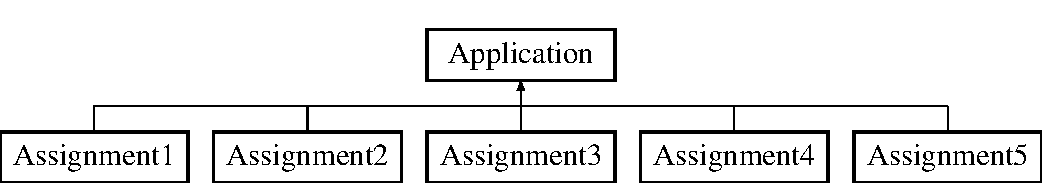
\includegraphics[height=2.000000cm]{class_application}
\end{center}
\end{figure}
\subsection*{Public Member Functions}
\begin{DoxyCompactItemize}
\item
\hyperlink{class_application_a78cdcb03e6f06272f7c528fe407951c5}{Application} (std\+::shared\+\_\+ptr$<$ class \hyperlink{class_scene}{Scene} $>$ input\+Scene, std\+::shared\+\_\+ptr$<$ class \hyperlink{class_camera}{Camera} $>$ input\+Camera)
\begin{DoxyCompactList}\small\item\em Create an application with a pre-\/allocated scene and camera. \end{DoxyCompactList}\item
virtual \hyperlink{class_application_a748bca84fefb9c12661cfaa2f623748d}{$\sim$\+Application} ()
\begin{DoxyCompactList}\small\item\em Virtual deconstrcutor to allow inheritance. \end{DoxyCompactList}\item
virtual void \hyperlink{class_application_a17cf1ea4552d26a1c20f7d98d793d41d}{Initialize} ()
\begin{DoxyCompactList}\small\item\em Initialization function to setup the stored camera and scene. \end{DoxyCompactList}\item
virtual std\+::unique\+\_\+ptr$<$ class \hyperlink{class_renderer}{Renderer} $>$ \hyperlink{class_application_a90c7fd9ecb6c8923948078903d442919}{Create\+Renderer} ()
\begin{DoxyCompactList}\small\item\em Creates a shared pointer of type \hyperlink{class_renderer}{Renderer}. \end{DoxyCompactList}\item
virtual glm\+::vec2 \hyperlink{class_application_ab190ae0e987fe95682714dd4b2495e82}{Get\+Window\+Size} () const
\begin{DoxyCompactList}\small\item\em Specifies the initial window size. \end{DoxyCompactList}\item
virtual bool \hyperlink{class_application_a454a1d926759c4bfac47e730570a7743}{Is\+Finished} () const
\begin{DoxyCompactList}\small\item\em Whether or not the application is finished running. \end{DoxyCompactList}\item
virtual void \hyperlink{class_application_a9cbe96f94653eae2bb6ad5857b00fa10}{Request\+Exit} ()
\begin{DoxyCompactList}\small\item\em Notifies the \hyperlink{class_application}{Application} that it should finish. \end{DoxyCompactList}\item
virtual void \hyperlink{class_application_a0800afd5651153d31fa775a8048d14dd}{Tick} (double delta\+Time)
\begin{DoxyCompactList}\small\item\em Called every frame to advance program logic. \end{DoxyCompactList}\item
virtual void \hyperlink{class_application_ae6074c3f102de1cb2fe4c81b545679db}{Handle\+Input} (S\+D\+L\+\_\+\+Keysym key, Uint32 state, Uint8 repeat, double timestamp, double delta\+Time)
\begin{DoxyCompactList}\small\item\em Processes an S\+DL keyboard event which has type \href{https://wiki.libsdl.org/SDL_KeyboardEvent}{\tt S\+D\+L\+\_\+\+Keyboard\+Event}. \end{DoxyCompactList}\item
virtual void \hyperlink{class_application_a74d92db64e051efa56d0357989dcb755}{Handle\+Window\+Event} (S\+D\+L\+\_\+\+Window\+Event\+ID event\+Id, Sint32 data1, Sint32 data2, double timestamp)
\begin{DoxyCompactList}\small\item\em Processes an S\+DL window event. Details about an S\+DL window event can be found \href{https://wiki.libsdl.org/SDL_WindowEvent}{\tt here} \end{DoxyCompactList}\end{DoxyCompactItemize}
\subsection*{Static Public Member Functions}
\begin{DoxyCompactItemize}
\item
static std\+::unique\+\_\+ptr$<$ \hyperlink{class_application}{Application} $>$ \hyperlink{class_application_a727f63f898a68bddf6d88309195ef194}{Create\+Application} (std\+::shared\+\_\+ptr$<$ class \hyperlink{class_scene}{Scene} $>$ \hyperlink{class_application_a88c6615107a5094bb93fa5f153f79554}{scene}, std\+::shared\+\_\+ptr$<$ class \hyperlink{class_camera}{Camera} $>$ \hyperlink{class_application_a0e8589fcb13c520ba472473abe5a518d}{camera})
\begin{DoxyCompactList}\small\item\em Creates a unique pointer to an \hyperlink{class_application}{Application}. This should be used instead of the constructor. \end{DoxyCompactList}\item
static std\+::shared\+\_\+ptr$<$ class \hyperlink{class_scene}{Scene} $>$ \hyperlink{class_application_a511e638cf5748e10151f17d6140b9119}{Create\+Scene} ()
\begin{DoxyCompactList}\small\item\em Creates a shared pointer of type \hyperlink{class_scene}{Scene}. \end{DoxyCompactList}\item
static std\+::shared\+\_\+ptr$<$ class \hyperlink{class_camera}{Camera} $>$ \hyperlink{class_application_a53c0a539fd2c4fe2cc48143cc0a3ea24}{Create\+Camera} ()
\begin{DoxyCompactList}\small\item\em Creates a shared pointer of type \hyperlink{class_camera}{Camera}. \end{DoxyCompactList}\end{DoxyCompactItemize}
\subsection*{Protected Member Functions}
\begin{DoxyCompactItemize}
\item
virtual void \hyperlink{class_application_abdba284a0f075ee1d4a2108c3a5236a2}{Handle\+Window\+Resize} (float x, float y)
\begin{DoxyCompactList}\small\item\em Called by \hyperlink{class_application_a74d92db64e051efa56d0357989dcb755}{Handle\+Window\+Event()} when the window is resized. \end{DoxyCompactList}\end{DoxyCompactItemize}
\subsection*{Protected Attributes}
\begin{DoxyCompactItemize}
\item
bool \hyperlink{class_application_ae1c1ff7a7663d9baa9b65a7ba8e1dcf8}{is\+Running}
\begin{DoxyCompactList}\small\item\em Whether or not the application is currently running. \end{DoxyCompactList}\item
std\+::shared\+\_\+ptr$<$ class \hyperlink{class_scene}{Scene} $>$ \hyperlink{class_application_a88c6615107a5094bb93fa5f153f79554}{scene}
\begin{DoxyCompactList}\small\item\em A shared pointer to the scene. \end{DoxyCompactList}\item
std\+::shared\+\_\+ptr$<$ class \hyperlink{class_camera}{Camera} $>$ \hyperlink{class_application_a0e8589fcb13c520ba472473abe5a518d}{camera}
\begin{DoxyCompactList}\small\item\em A shared pointer to the camera. \end{DoxyCompactList}\end{DoxyCompactItemize}
\subsection*{Private Member Functions}
\begin{DoxyCompactItemize}
\item
virtual void \hyperlink{class_application_aa8e8017ef8dd86293c96d0645e66d440}{Setup\+Scene} ()
\begin{DoxyCompactList}\small\item\em Called by \hyperlink{class_application_a17cf1ea4552d26a1c20f7d98d793d41d}{Initialize()} to populate the scene. \end{DoxyCompactList}\item
virtual void \hyperlink{class_application_a2eb61ca027f223a5c5ad1bf982481193}{Setup\+Camera} ()
\begin{DoxyCompactList}\small\item\em Called by \hyperlink{class_application_a17cf1ea4552d26a1c20f7d98d793d41d}{Initialize()} to setup the camera. \end{DoxyCompactList}\end{DoxyCompactItemize}


\subsection{Detailed Description}
Handles creating configurable objects (i.\+e. scene, camera, renderer), handling S\+DL events passed in by the \hyperlink{class_media_layer}{Media\+Layer}, and handles creating the scene to be display.

An \textquotesingle{}\hyperlink{class_application}{Application}\textquotesingle{} M\+U\+ST be created to run the assignment framework. By default, the application will create a 1280x720 window that is completely black. After the \textquotesingle{}\hyperlink{class_application}{Application}\textquotesingle{} is created, it must be passed to the \textquotesingle{}\hyperlink{class_media_layer}{Media\+Layer}\textquotesingle{} who will call the \textquotesingle{}\hyperlink{class_application}{Application}\textquotesingle{}s tick function every frame.

\subsection{Constructor \& Destructor Documentation}
\hypertarget{class_application_a78cdcb03e6f06272f7c528fe407951c5}{}\label{class_application_a78cdcb03e6f06272f7c528fe407951c5}
\index{Application@{Application}!Application@{Application}}
\index{Application@{Application}!Application@{Application}}
\subsubsection{\texorpdfstring{Application()}{Application()}}
{\footnotesize\ttfamily Application\+::\+Application (\begin{DoxyParamCaption}\item[{std\+::shared\+\_\+ptr$<$ class \hyperlink{class_scene}{Scene} $>$}]{input\+Scene,  }\item[{std\+::shared\+\_\+ptr$<$ class \hyperlink{class_camera}{Camera} $>$}]{input\+Camera }\end{DoxyParamCaption})}



Create an application with a pre-\/allocated scene and camera.


\begin{DoxyParams}{Parameters}
{\em input\+Scene} & A pre-\/allocated scene. This should be generated using \hyperlink{class_application_a511e638cf5748e10151f17d6140b9119}{Create\+Scene()} in the appropriate subclass. \\
\hline
{\em input\+Camera} & A pre-\/allocated camera. This should be generated using \hyperlink{class_application_a53c0a539fd2c4fe2cc48143cc0a3ea24}{Create\+Camera()} in the appropriate subclass. \\
\hline
\end{DoxyParams}
\begin{DoxyWarning}{Warning}
Do not use directly. Use Create\+Application instead.
\end{DoxyWarning}
\hypertarget{class_application_a748bca84fefb9c12661cfaa2f623748d}{}\label{class_application_a748bca84fefb9c12661cfaa2f623748d}
\index{Application@{Application}!````~Application@{$\sim$\+Application}}
\index{````~Application@{$\sim$\+Application}!Application@{Application}}
\subsubsection{\texorpdfstring{$\sim$\+Application()}{~Application()}}
{\footnotesize\ttfamily Application\+::$\sim$\+Application (\begin{DoxyParamCaption}{ }\end{DoxyParamCaption})\hspace{0.3cm}{\ttfamily [virtual]}}



Virtual deconstrcutor to allow inheritance.



\subsection{Member Function Documentation}
\hypertarget{class_application_a727f63f898a68bddf6d88309195ef194}{}\label{class_application_a727f63f898a68bddf6d88309195ef194}
\index{Application@{Application}!Create\+Application@{Create\+Application}}
\index{Create\+Application@{Create\+Application}!Application@{Application}}
\subsubsection{\texorpdfstring{Create\+Application()}{CreateApplication()}}
{\footnotesize\ttfamily std\+::unique\+\_\+ptr$<$ \hyperlink{class_application}{Application} $>$ Application\+::\+Create\+Application (\begin{DoxyParamCaption}\item[{std\+::shared\+\_\+ptr$<$ class \hyperlink{class_scene}{Scene} $>$}]{scene,  }\item[{std\+::shared\+\_\+ptr$<$ class \hyperlink{class_camera}{Camera} $>$}]{camera }\end{DoxyParamCaption})\hspace{0.3cm}{\ttfamily [static]}}



Creates a unique pointer to an \hyperlink{class_application}{Application}. This should be used instead of the constructor.

\begin{DoxyReturn}{Returns}
A unique pointer to an \hyperlink{class_application}{Application}.
\end{DoxyReturn}
See \hyperlink{class_application_a78cdcb03e6f06272f7c528fe407951c5}{Application()} for more details. \hypertarget{class_application_a53c0a539fd2c4fe2cc48143cc0a3ea24}{}\label{class_application_a53c0a539fd2c4fe2cc48143cc0a3ea24}
\index{Application@{Application}!Create\+Camera@{Create\+Camera}}
\index{Create\+Camera@{Create\+Camera}!Application@{Application}}
\subsubsection{\texorpdfstring{Create\+Camera()}{CreateCamera()}}
{\footnotesize\ttfamily std\+::shared\+\_\+ptr$<$ \hyperlink{class_camera}{Camera} $>$ Application\+::\+Create\+Camera (\begin{DoxyParamCaption}{ }\end{DoxyParamCaption})\hspace{0.3cm}{\ttfamily [static]}}



Creates a shared pointer of type \hyperlink{class_camera}{Camera}.

\begin{DoxyReturn}{Returns}
A shared pointer to a \hyperlink{class_camera}{Camera}.
\end{DoxyReturn}
The subclass should also create a function \hyperlink{class_application_a53c0a539fd2c4fe2cc48143cc0a3ea24}{Create\+Camera()} that returns the proper type of \hyperlink{class_camera}{Camera} to create. \hypertarget{class_application_a90c7fd9ecb6c8923948078903d442919}{}\label{class_application_a90c7fd9ecb6c8923948078903d442919}
\index{Application@{Application}!Create\+Renderer@{Create\+Renderer}}
\index{Create\+Renderer@{Create\+Renderer}!Application@{Application}}
\subsubsection{\texorpdfstring{Create\+Renderer()}{CreateRenderer()}}
{\footnotesize\ttfamily std\+::unique\+\_\+ptr$<$ class \hyperlink{class_renderer}{Renderer} $>$ Application\+::\+Create\+Renderer (\begin{DoxyParamCaption}{ }\end{DoxyParamCaption})\hspace{0.3cm}{\ttfamily [virtual]}}



Creates a shared pointer of type \hyperlink{class_renderer}{Renderer}.

\begin{DoxyReturn}{Returns}
A unique pointer to a \hyperlink{class_renderer}{Renderer}.
\end{DoxyReturn}
The subclass should override this function \hyperlink{class_application_a90c7fd9ecb6c8923948078903d442919}{Create\+Renderer()} to return the proper type of \hyperlink{class_renderer}{Renderer} to create. \hypertarget{class_application_a511e638cf5748e10151f17d6140b9119}{}\label{class_application_a511e638cf5748e10151f17d6140b9119}
\index{Application@{Application}!Create\+Scene@{Create\+Scene}}
\index{Create\+Scene@{Create\+Scene}!Application@{Application}}
\subsubsection{\texorpdfstring{Create\+Scene()}{CreateScene()}}
{\footnotesize\ttfamily std\+::shared\+\_\+ptr$<$ \hyperlink{class_scene}{Scene} $>$ Application\+::\+Create\+Scene (\begin{DoxyParamCaption}{ }\end{DoxyParamCaption})\hspace{0.3cm}{\ttfamily [static]}}



Creates a shared pointer of type \hyperlink{class_scene}{Scene}.

\begin{DoxyReturn}{Returns}
A shared pointer to a \hyperlink{class_scene}{Scene}.
\end{DoxyReturn}
The subclass should also create a function \hyperlink{class_application_a511e638cf5748e10151f17d6140b9119}{Create\+Scene()} that returns the proper type of \hyperlink{class_scene}{Scene} to create. \hypertarget{class_application_ab190ae0e987fe95682714dd4b2495e82}{}\label{class_application_ab190ae0e987fe95682714dd4b2495e82}
\index{Application@{Application}!Get\+Window\+Size@{Get\+Window\+Size}}
\index{Get\+Window\+Size@{Get\+Window\+Size}!Application@{Application}}
\subsubsection{\texorpdfstring{Get\+Window\+Size()}{GetWindowSize()}}
{\footnotesize\ttfamily glm\+::vec2 Application\+::\+Get\+Window\+Size (\begin{DoxyParamCaption}{ }\end{DoxyParamCaption}) const\hspace{0.3cm}{\ttfamily [virtual]}}



Specifies the initial window size.

\begin{DoxyReturn}{Returns}
The desired window size.
\end{DoxyReturn}


Reimplemented in \hyperlink{class_assignment2_a9ea79bd468c12dde5159ca7b8efd8e1e}{Assignment2}, \hyperlink{class_assignment3_aec48ba5500d906963fdac555ee47cb72}{Assignment3}, \hyperlink{class_assignment4_ad197b75e730f9b32458429df8d55458e}{Assignment4}, \hyperlink{class_assignment5_ac199b6149ffa3dbedc7e0d49bb24c628}{Assignment5}, and \hyperlink{class_assignment1_a581b6c897c918eede3f9bbb1cbc50320}{Assignment1}.

\hypertarget{class_application_ae6074c3f102de1cb2fe4c81b545679db}{}\label{class_application_ae6074c3f102de1cb2fe4c81b545679db}
\index{Application@{Application}!Handle\+Input@{Handle\+Input}}
\index{Handle\+Input@{Handle\+Input}!Application@{Application}}
\subsubsection{\texorpdfstring{Handle\+Input()}{HandleInput()}}
{\footnotesize\ttfamily void Application\+::\+Handle\+Input (\begin{DoxyParamCaption}\item[{S\+D\+L\+\_\+\+Keysym}]{key,  }\item[{Uint32}]{state,  }\item[{Uint8}]{repeat,  }\item[{double}]{timestamp,  }\item[{double}]{delta\+Time }\end{DoxyParamCaption})\hspace{0.3cm}{\ttfamily [virtual]}}



Processes an S\+DL keyboard event which has type \href{https://wiki.libsdl.org/SDL_KeyboardEvent}{\tt S\+D\+L\+\_\+\+Keyboard\+Event}.


\begin{DoxyParams}{Parameters}
{\em key} & See the S\+DL documentation for more details about \href{https://wiki.libsdl.org/SDL_Keysym}{\tt S\+D\+L\+\_\+\+Keysym}. \\
\hline
{\em state} & This is the type field in the \href{https://wiki.libsdl.org/SDL_Event}{\tt S\+D\+L\+\_\+\+Event}datastructure. \\
\hline
{\em repeat} & This value is non-\/zero is the key is being repeated. \\
\hline
{\em timestamp} & Timestamp is the number of seconds since the program was first started. \\
\hline
{\em delta\+Time} & The amount of time (in seconds) since the last tick.\\
\hline
\end{DoxyParams}
Takes in a keyboard event and process it. This does nothing by default. \textquotesingle{}delta\+Time\textquotesingle{} is included to allow you to move something and have the movement look smooth. For example, if you have an object that you want to move forward whenever \textquotesingle{}W\textquotesingle{} is pressed. You know that the object travels at 10 meters per second when \textquotesingle{}W\textquotesingle{} is pressed and 0 meters per second when it is not. How far should you move the object? You would want to move it forward by $10 \cdot deltaTime $ units.

Reimplemented in \hyperlink{class_assignment2_a3ee099a8ba45db14103541981e3c4fe8}{Assignment2}, \hyperlink{class_assignment3_a1cc65ca321f39eb7092959b2dada8d31}{Assignment3}, \hyperlink{class_assignment4_a02c51d46e2cbb55e7963b6bfbedaf1c4}{Assignment4}, \hyperlink{class_assignment5_aab8f8440144665db9aafd7ca1cf55cff}{Assignment5}, and \hyperlink{class_assignment1_ab9db4f51e177dd72130cd61d86b97535}{Assignment1}.

\hypertarget{class_application_a74d92db64e051efa56d0357989dcb755}{}\label{class_application_a74d92db64e051efa56d0357989dcb755}
\index{Application@{Application}!Handle\+Window\+Event@{Handle\+Window\+Event}}
\index{Handle\+Window\+Event@{Handle\+Window\+Event}!Application@{Application}}
\subsubsection{\texorpdfstring{Handle\+Window\+Event()}{HandleWindowEvent()}}
{\footnotesize\ttfamily void Application\+::\+Handle\+Window\+Event (\begin{DoxyParamCaption}\item[{S\+D\+L\+\_\+\+Window\+Event\+ID}]{event\+Id,  }\item[{Sint32}]{data1,  }\item[{Sint32}]{data2,  }\item[{double}]{timestamp }\end{DoxyParamCaption})\hspace{0.3cm}{\ttfamily [virtual]}}



Processes an S\+DL window event. Details about an S\+DL window event can be found \href{https://wiki.libsdl.org/SDL_WindowEvent}{\tt here}


\begin{DoxyParams}{Parameters}
{\em event\+Id} & This is an \href{https://wiki.libsdl.org/SDL_WindowEventID}{\tt S\+D\+L\+\_\+\+Window\+Event\+ID}. See the S\+DL documentation for more details. \\
\hline
{\em data1} & This changes depending on what event\+Id is. See the docs for S\+D\+L\+\_\+\+Window\+Event\+ID. \\
\hline
{\em data2} & This changes depending on what event\+Id is. See the docs for S\+D\+L\+\_\+\+Window\+Event\+ID. \\
\hline
{\em timestamp} & Timestamp is the number of seconds since the program was first started.\\
\hline
\end{DoxyParams}
This takes in a window event and process it. By default it handles when the size of the window change and calls \hyperlink{class_application_abdba284a0f075ee1d4a2108c3a5236a2}{Handle\+Window\+Resize()}. You can expand on this functionality in the sub-\/class to handle other events such as the window moving, etc. However, make sure you maintain a call to \hyperlink{class_application_a74d92db64e051efa56d0357989dcb755}{Application\+::\+Handle\+Window\+Event()} to make sure gl\+Viewport is still called! \hypertarget{class_application_abdba284a0f075ee1d4a2108c3a5236a2}{}\label{class_application_abdba284a0f075ee1d4a2108c3a5236a2}
\index{Application@{Application}!Handle\+Window\+Resize@{Handle\+Window\+Resize}}
\index{Handle\+Window\+Resize@{Handle\+Window\+Resize}!Application@{Application}}
\subsubsection{\texorpdfstring{Handle\+Window\+Resize()}{HandleWindowResize()}}
{\footnotesize\ttfamily void Application\+::\+Handle\+Window\+Resize (\begin{DoxyParamCaption}\item[{float}]{x,  }\item[{float}]{y }\end{DoxyParamCaption})\hspace{0.3cm}{\ttfamily [protected]}, {\ttfamily [virtual]}}



Called by \hyperlink{class_application_a74d92db64e051efa56d0357989dcb755}{Handle\+Window\+Event()} when the window is resized.


\begin{DoxyParams}{Parameters}
{\em x} & The width of the window. \\
\hline
{\em y} & The height of the window.\\
\hline
\end{DoxyParams}
By default calls, \href{https://www.opengl.org/sdk/docs/man/html/glViewport.xhtml}{\tt gl\+Viewport} to resize the viewport as necessary. If any part of your application depends on the window resize, you will want to take care of it in this function! (Hint for the O\+P\+T\+I\+O\+N\+AL deferred rendering task in assignment 2\+: your \textquotesingle{}G-\/\+Buffers\textquotesingle{} should be resized).

Reimplemented in \hyperlink{class_assignment2_a1af734567de5e8e73a2fd726fe3914f2}{Assignment2}, \hyperlink{class_assignment3_a851c637c83c8092d8adfb5c9f761daeb}{Assignment3}, \hyperlink{class_assignment4_ac79558272dc476db3ee4a99793f401f2}{Assignment4}, and \hyperlink{class_assignment5_a0e7325af72d41b95f9a19ebe1440e756}{Assignment5}.

\hypertarget{class_application_a17cf1ea4552d26a1c20f7d98d793d41d}{}\label{class_application_a17cf1ea4552d26a1c20f7d98d793d41d}
\index{Application@{Application}!Initialize@{Initialize}}
\index{Initialize@{Initialize}!Application@{Application}}
\subsubsection{\texorpdfstring{Initialize()}{Initialize()}}
{\footnotesize\ttfamily void Application\+::\+Initialize (\begin{DoxyParamCaption}{ }\end{DoxyParamCaption})\hspace{0.3cm}{\ttfamily [virtual]}}



Initialization function to setup the stored camera and scene.

This initialization function exists because the \hyperlink{class_application_aa8e8017ef8dd86293c96d0645e66d440}{Setup\+Scene()} and \hyperlink{class_application_a2eb61ca027f223a5c5ad1bf982481193}{Setup\+Camera()} functions are virtual and thus can not exist within the constructor. This function is called in \hyperlink{class_media_layer_aea3b3bc36411af90517692b110d2829a}{Media\+Layer\+::\+Media\+Layer()}. \hypertarget{class_application_a454a1d926759c4bfac47e730570a7743}{}\label{class_application_a454a1d926759c4bfac47e730570a7743}
\index{Application@{Application}!Is\+Finished@{Is\+Finished}}
\index{Is\+Finished@{Is\+Finished}!Application@{Application}}
\subsubsection{\texorpdfstring{Is\+Finished()}{IsFinished()}}
{\footnotesize\ttfamily bool Application\+::\+Is\+Finished (\begin{DoxyParamCaption}{ }\end{DoxyParamCaption}) const\hspace{0.3cm}{\ttfamily [virtual]}}



Whether or not the application is finished running.

\begin{DoxyReturn}{Returns}
Whether the application is finished running.
\end{DoxyReturn}
When the \hyperlink{class_media_layer_a570ff8c3fc3e8f3e720d9dcebafba143}{Media\+Layer\+::\+Tick()} function detects that the application is finished, the program will exit. \hypertarget{class_application_a9cbe96f94653eae2bb6ad5857b00fa10}{}\label{class_application_a9cbe96f94653eae2bb6ad5857b00fa10}
\index{Application@{Application}!Request\+Exit@{Request\+Exit}}
\index{Request\+Exit@{Request\+Exit}!Application@{Application}}
\subsubsection{\texorpdfstring{Request\+Exit()}{RequestExit()}}
{\footnotesize\ttfamily void Application\+::\+Request\+Exit (\begin{DoxyParamCaption}{ }\end{DoxyParamCaption})\hspace{0.3cm}{\ttfamily [virtual]}}



Notifies the \hyperlink{class_application}{Application} that it should finish.

An external source (i.\+e. the \hyperlink{class_media_layer}{Media\+Layer}) may request for the \hyperlink{class_application}{Application} to finish. This lets the \hyperlink{class_application}{Application} exit gracefully. The \hyperlink{class_application}{Application} can choose to ignore the request (thought that is not recommended). After this function is called, \hyperlink{class_application_a454a1d926759c4bfac47e730570a7743}{Is\+Finished()} should return true. \hypertarget{class_application_a2eb61ca027f223a5c5ad1bf982481193}{}\label{class_application_a2eb61ca027f223a5c5ad1bf982481193}
\index{Application@{Application}!Setup\+Camera@{Setup\+Camera}}
\index{Setup\+Camera@{Setup\+Camera}!Application@{Application}}
\subsubsection{\texorpdfstring{Setup\+Camera()}{SetupCamera()}}
{\footnotesize\ttfamily void Application\+::\+Setup\+Camera (\begin{DoxyParamCaption}{ }\end{DoxyParamCaption})\hspace{0.3cm}{\ttfamily [private]}, {\ttfamily [virtual]}}



Called by \hyperlink{class_application_a17cf1ea4552d26a1c20f7d98d793d41d}{Initialize()} to setup the camera.

Note by the time this function is called, the \hyperlink{class_application}{Application} sub-\/class is fully constructed and \hyperlink{class_camera}{Camera} object is already created.

Reimplemented in \hyperlink{class_assignment2_ab9ace1ffdac8f7425c64d661f3d13acd}{Assignment2}, \hyperlink{class_assignment3_a1d23eb19973b78e516169f4a03954526}{Assignment3}, \hyperlink{class_assignment4_aa2bc15adb48cf54e477fce0c686cf2f0}{Assignment4}, and \hyperlink{class_assignment5_a0c49123e133adfb36c769c943eae42fa}{Assignment5}.

\hypertarget{class_application_aa8e8017ef8dd86293c96d0645e66d440}{}\label{class_application_aa8e8017ef8dd86293c96d0645e66d440}
\index{Application@{Application}!Setup\+Scene@{Setup\+Scene}}
\index{Setup\+Scene@{Setup\+Scene}!Application@{Application}}
\subsubsection{\texorpdfstring{Setup\+Scene()}{SetupScene()}}
{\footnotesize\ttfamily void Application\+::\+Setup\+Scene (\begin{DoxyParamCaption}{ }\end{DoxyParamCaption})\hspace{0.3cm}{\ttfamily [private]}, {\ttfamily [virtual]}}



Called by \hyperlink{class_application_a17cf1ea4552d26a1c20f7d98d793d41d}{Initialize()} to populate the scene.

Note by the time this function is called, the \hyperlink{class_application}{Application} sub-\/class is fully constructed and \hyperlink{class_scene}{Scene} object is already created.

Reimplemented in \hyperlink{class_assignment2_aa4f8ccd09a7accbdf093394c6ee4f63f}{Assignment2}, \hyperlink{class_assignment3_a2dc29d9016a9d822ede84b9ef41429a5}{Assignment3}, \hyperlink{class_assignment4_a38c50647bb65ff03aaf293fcc21dc5fd}{Assignment4}, \hyperlink{class_assignment5_a43328e09e6241ae6c62a9b7be7659b3b}{Assignment5}, and \hyperlink{class_assignment1_a8d12cf21f1463caa5a8da45110b50103}{Assignment1}.

\hypertarget{class_application_a0800afd5651153d31fa775a8048d14dd}{}\label{class_application_a0800afd5651153d31fa775a8048d14dd}
\index{Application@{Application}!Tick@{Tick}}
\index{Tick@{Tick}!Application@{Application}}
\subsubsection{\texorpdfstring{Tick()}{Tick()}}
{\footnotesize\ttfamily void Application\+::\+Tick (\begin{DoxyParamCaption}\item[{double}]{delta\+Time }\end{DoxyParamCaption})\hspace{0.3cm}{\ttfamily [virtual]}}



Called every frame to advance program logic.


\begin{DoxyParams}{Parameters}
{\em delta\+Time} & The amount of time (in seconds) since the last tick.\\
\hline
\end{DoxyParams}
If you need something in the \hyperlink{class_scene}{Scene} to change over time, this is where you should implement that logic. It is recommended that you make use of the delta\+Time variable to make things change smoothly!

Reimplemented in \hyperlink{class_assignment2_a41544ad361dd798d5fae1ec3197fc66e}{Assignment2}, \hyperlink{class_assignment3_a11256b6e7b38ab24baa92729cfb8ffe2}{Assignment3}, \hyperlink{class_assignment4_a3ef3fef7a6ae13603bc453b29e079c5d}{Assignment4}, and \hyperlink{class_assignment5_a34cdf7bc962c3a0e3959c77a24c54d79}{Assignment5}.



\subsection{Member Data Documentation}
\hypertarget{class_application_a0e8589fcb13c520ba472473abe5a518d}{}\label{class_application_a0e8589fcb13c520ba472473abe5a518d}
\index{Application@{Application}!camera@{camera}}
\index{camera@{camera}!Application@{Application}}
\subsubsection{\texorpdfstring{camera}{camera}}
{\footnotesize\ttfamily std\+::shared\+\_\+ptr$<$class \hyperlink{class_camera}{Camera}$>$ Application\+::camera\hspace{0.3cm}{\ttfamily [protected]}}



A shared pointer to the camera.

Currently, only one camera is supported at a time. This one camera will be shared across the framework to properly generate the view and projection matrices. Additionally, shaders utilize some camera properties to calculate the fragment color. \hypertarget{class_application_ae1c1ff7a7663d9baa9b65a7ba8e1dcf8}{}\label{class_application_ae1c1ff7a7663d9baa9b65a7ba8e1dcf8}
\index{Application@{Application}!is\+Running@{is\+Running}}
\index{is\+Running@{is\+Running}!Application@{Application}}
\subsubsection{\texorpdfstring{is\+Running}{isRunning}}
{\footnotesize\ttfamily bool Application\+::is\+Running\hspace{0.3cm}{\ttfamily [protected]}}



Whether or not the application is currently running.

This variable is negated and returned by \hyperlink{class_application_a454a1d926759c4bfac47e730570a7743}{Is\+Finished()}. \hypertarget{class_application_a88c6615107a5094bb93fa5f153f79554}{}\label{class_application_a88c6615107a5094bb93fa5f153f79554}
\index{Application@{Application}!scene@{scene}}
\index{scene@{scene}!Application@{Application}}
\subsubsection{\texorpdfstring{scene}{scene}}
{\footnotesize\ttfamily std\+::shared\+\_\+ptr$<$class \hyperlink{class_scene}{Scene}$>$ Application\+::scene\hspace{0.3cm}{\ttfamily [protected]}}



A shared pointer to the scene.

Currently, there can only ever be one scene at a time. You will add lights and other objects to the scene to generate your image. This scene is used across the framework to perform rendering.

The documentation for this class was generated from the following files\+:\begin{DoxyCompactItemize}
\item
/data/MO814A-MC937A/MO814A-MC937Aopengl-\/instructor/source/common/\hyperlink{_application_8h}{Application.\+h}\item
/data/MO814A-MC937A/MO814A-MC937Aopengl-\/instructor/source/common/\hyperlink{_application_8cpp}{Application.\+cpp}\end{DoxyCompactItemize}

\hypertarget{class_assignment1}{}\section{Assignment1 Class Reference}
\label{class_assignment1}\index{Assignment1@{Assignment1}}


{\ttfamily \#include $<$Assignment1.\+h$>$}

Inheritance diagram for Assignment1\+:\begin{figure}[H]
\begin{center}
\leavevmode
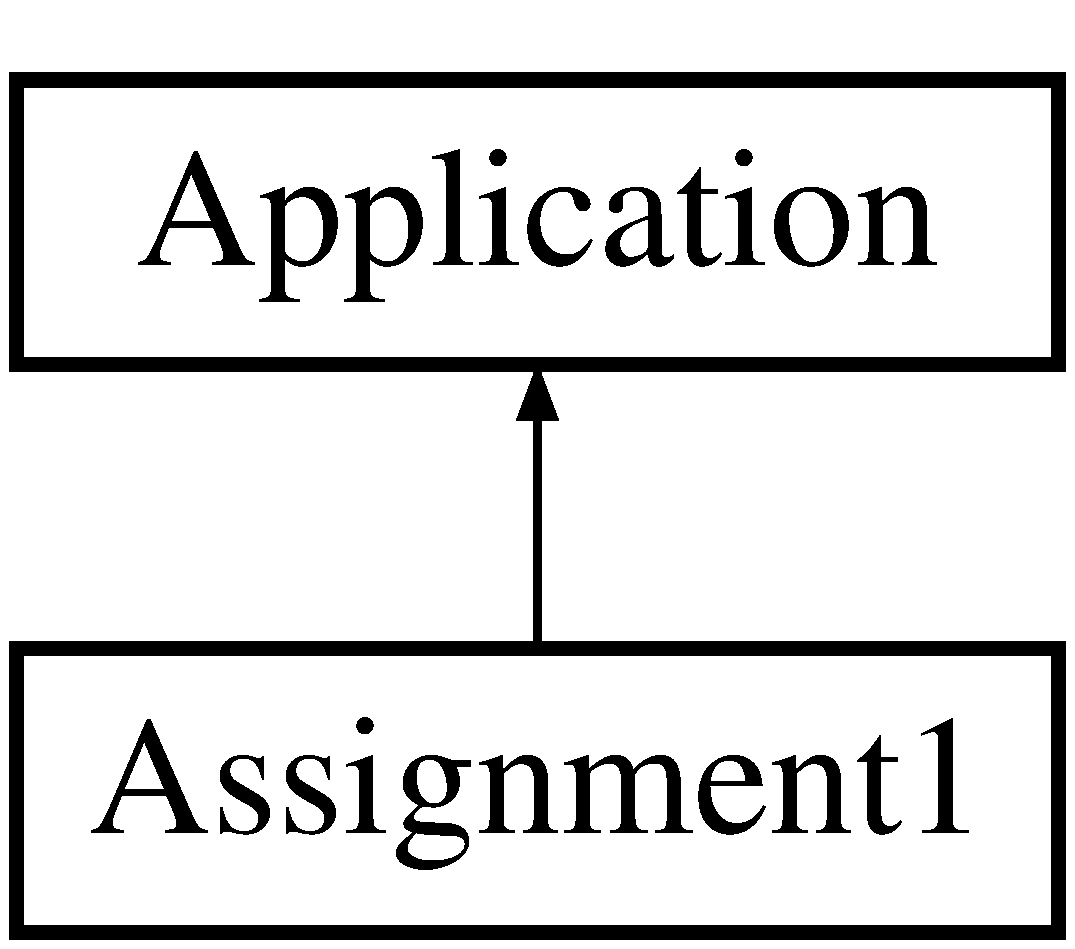
\includegraphics[height=2.000000cm]{class_assignment1}
\end{center}
\end{figure}
\subsection*{Public Member Functions}
\begin{DoxyCompactItemize}
\item
\hyperlink{class_assignment1_ade9ef18c233dab37d37f20760fe7674d}{Assignment1} (std\+::shared\+\_\+ptr$<$ class \hyperlink{class_scene}{Scene} $>$ input\+Scene, std\+::shared\+\_\+ptr$<$ class \hyperlink{class_camera}{Camera} $>$ input\+Camera)
\item
virtual glm\+::vec2 \hyperlink{class_assignment1_a581b6c897c918eede3f9bbb1cbc50320}{Get\+Window\+Size} () const
\begin{DoxyCompactList}\small\item\em Specifies the initial window size. \end{DoxyCompactList}\item
virtual void \hyperlink{class_assignment1_ab9db4f51e177dd72130cd61d86b97535}{Handle\+Input} (S\+D\+L\+\_\+\+Keysym key, Uint32 state, Uint8 repeat, double timestamp, double delta\+Time)
\begin{DoxyCompactList}\small\item\em Processes an S\+DL keyboard event which has type \href{https://wiki.libsdl.org/SDL_KeyboardEvent}{\tt S\+D\+L\+\_\+\+Keyboard\+Event}. \end{DoxyCompactList}\end{DoxyCompactItemize}
\subsection*{Static Public Member Functions}
\begin{DoxyCompactItemize}
\item
static std\+::unique\+\_\+ptr$<$ \hyperlink{class_application}{Application} $>$ \hyperlink{class_assignment1_ae1952b4904620a16c4f2c098bf061c68}{Create\+Application} (std\+::shared\+\_\+ptr$<$ class \hyperlink{class_scene}{Scene} $>$ \hyperlink{class_application_a88c6615107a5094bb93fa5f153f79554}{scene}, std\+::shared\+\_\+ptr$<$ class \hyperlink{class_camera}{Camera} $>$ \hyperlink{class_application_a0e8589fcb13c520ba472473abe5a518d}{camera})
\end{DoxyCompactItemize}
\subsection*{Private Member Functions}
\begin{DoxyCompactItemize}
\item
virtual void \hyperlink{class_assignment1_a8d12cf21f1463caa5a8da45110b50103}{Setup\+Scene} ()
\begin{DoxyCompactList}\small\item\em Called by \hyperlink{class_application_a17cf1ea4552d26a1c20f7d98d793d41d}{Initialize()} to populate the scene. \end{DoxyCompactList}\item
virtual void \hyperlink{class_assignment1_a07743a6d86f7603dd58339c4db1de192}{Setup\+Example1} ()
\item
virtual void \hyperlink{class_assignment1_aeabed7b579d59a6fdacaeab468afba29}{Setup\+Example2} ()
\item
virtual void \hyperlink{class_assignment1_afbb3cb7765b899e69c9847d29f045392}{Setup\+Example3} ()
\end{DoxyCompactItemize}
\subsection*{Additional Inherited Members}


\subsection{Constructor \& Destructor Documentation}
\hypertarget{class_assignment1_ade9ef18c233dab37d37f20760fe7674d}{}\label{class_assignment1_ade9ef18c233dab37d37f20760fe7674d}
\index{Assignment1@{Assignment1}!Assignment1@{Assignment1}}
\index{Assignment1@{Assignment1}!Assignment1@{Assignment1}}
\subsubsection{\texorpdfstring{Assignment1()}{Assignment1()}}
{\footnotesize\ttfamily Assignment1\+::\+Assignment1 (\begin{DoxyParamCaption}\item[{std\+::shared\+\_\+ptr$<$ class \hyperlink{class_scene}{Scene} $>$}]{input\+Scene,  }\item[{std\+::shared\+\_\+ptr$<$ class \hyperlink{class_camera}{Camera} $>$}]{input\+Camera }\end{DoxyParamCaption})}



\subsection{Member Function Documentation}
\hypertarget{class_assignment1_ae1952b4904620a16c4f2c098bf061c68}{}\label{class_assignment1_ae1952b4904620a16c4f2c098bf061c68}
\index{Assignment1@{Assignment1}!Create\+Application@{Create\+Application}}
\index{Create\+Application@{Create\+Application}!Assignment1@{Assignment1}}
\subsubsection{\texorpdfstring{Create\+Application()}{CreateApplication()}}
{\footnotesize\ttfamily std\+::unique\+\_\+ptr$<$ \hyperlink{class_application}{Application} $>$ Assignment1\+::\+Create\+Application (\begin{DoxyParamCaption}\item[{std\+::shared\+\_\+ptr$<$ class \hyperlink{class_scene}{Scene} $>$}]{scene,  }\item[{std\+::shared\+\_\+ptr$<$ class \hyperlink{class_camera}{Camera} $>$}]{camera }\end{DoxyParamCaption})\hspace{0.3cm}{\ttfamily [static]}}

\hypertarget{class_assignment1_a581b6c897c918eede3f9bbb1cbc50320}{}\label{class_assignment1_a581b6c897c918eede3f9bbb1cbc50320}
\index{Assignment1@{Assignment1}!Get\+Window\+Size@{Get\+Window\+Size}}
\index{Get\+Window\+Size@{Get\+Window\+Size}!Assignment1@{Assignment1}}
\subsubsection{\texorpdfstring{Get\+Window\+Size()}{GetWindowSize()}}
{\footnotesize\ttfamily glm\+::vec2 Assignment1\+::\+Get\+Window\+Size (\begin{DoxyParamCaption}{ }\end{DoxyParamCaption}) const\hspace{0.3cm}{\ttfamily [virtual]}}



Specifies the initial window size.

\begin{DoxyReturn}{Returns}
The desired window size.
\end{DoxyReturn}


Reimplemented from \hyperlink{class_application_ab190ae0e987fe95682714dd4b2495e82}{Application}.

\hypertarget{class_assignment1_ab9db4f51e177dd72130cd61d86b97535}{}\label{class_assignment1_ab9db4f51e177dd72130cd61d86b97535}
\index{Assignment1@{Assignment1}!Handle\+Input@{Handle\+Input}}
\index{Handle\+Input@{Handle\+Input}!Assignment1@{Assignment1}}
\subsubsection{\texorpdfstring{Handle\+Input()}{HandleInput()}}
{\footnotesize\ttfamily void Assignment1\+::\+Handle\+Input (\begin{DoxyParamCaption}\item[{S\+D\+L\+\_\+\+Keysym}]{key,  }\item[{Uint32}]{state,  }\item[{Uint8}]{repeat,  }\item[{double}]{timestamp,  }\item[{double}]{delta\+Time }\end{DoxyParamCaption})\hspace{0.3cm}{\ttfamily [virtual]}}



Processes an S\+DL keyboard event which has type \href{https://wiki.libsdl.org/SDL_KeyboardEvent}{\tt S\+D\+L\+\_\+\+Keyboard\+Event}.


\begin{DoxyParams}{Parameters}
{\em key} & See the S\+DL documentation for more details about \href{https://wiki.libsdl.org/SDL_Keysym}{\tt S\+D\+L\+\_\+\+Keysym}. \\
\hline
{\em state} & This is the type field in the \href{https://wiki.libsdl.org/SDL_Event}{\tt S\+D\+L\+\_\+\+Event}datastructure. \\
\hline
{\em repeat} & This value is non-\/zero is the key is being repeated. \\
\hline
{\em timestamp} & Timestamp is the number of seconds since the program was first started. \\
\hline
{\em delta\+Time} & The amount of time (in seconds) since the last tick.\\
\hline
\end{DoxyParams}
Takes in a keyboard event and process it. This does nothing by default. \textquotesingle{}delta\+Time\textquotesingle{} is included to allow you to move something and have the movement look smooth. For example, if you have an object that you want to move forward whenever \textquotesingle{}W\textquotesingle{} is pressed. You know that the object travels at 10 meters per second when \textquotesingle{}W\textquotesingle{} is pressed and 0 meters per second when it is not. How far should you move the object? You would want to move it forward by $10 \cdot deltaTime $ units.

Reimplemented from \hyperlink{class_application_ae6074c3f102de1cb2fe4c81b545679db}{Application}.

\hypertarget{class_assignment1_a07743a6d86f7603dd58339c4db1de192}{}\label{class_assignment1_a07743a6d86f7603dd58339c4db1de192}
\index{Assignment1@{Assignment1}!Setup\+Example1@{Setup\+Example1}}
\index{Setup\+Example1@{Setup\+Example1}!Assignment1@{Assignment1}}
\subsubsection{\texorpdfstring{Setup\+Example1()}{SetupExample1()}}
{\footnotesize\ttfamily void Assignment1\+::\+Setup\+Example1 (\begin{DoxyParamCaption}{ }\end{DoxyParamCaption})\hspace{0.3cm}{\ttfamily [private]}, {\ttfamily [virtual]}}

\hypertarget{class_assignment1_aeabed7b579d59a6fdacaeab468afba29}{}\label{class_assignment1_aeabed7b579d59a6fdacaeab468afba29}
\index{Assignment1@{Assignment1}!Setup\+Example2@{Setup\+Example2}}
\index{Setup\+Example2@{Setup\+Example2}!Assignment1@{Assignment1}}
\subsubsection{\texorpdfstring{Setup\+Example2()}{SetupExample2()}}
{\footnotesize\ttfamily void Assignment1\+::\+Setup\+Example2 (\begin{DoxyParamCaption}{ }\end{DoxyParamCaption})\hspace{0.3cm}{\ttfamily [private]}, {\ttfamily [virtual]}}

\hypertarget{class_assignment1_afbb3cb7765b899e69c9847d29f045392}{}\label{class_assignment1_afbb3cb7765b899e69c9847d29f045392}
\index{Assignment1@{Assignment1}!Setup\+Example3@{Setup\+Example3}}
\index{Setup\+Example3@{Setup\+Example3}!Assignment1@{Assignment1}}
\subsubsection{\texorpdfstring{Setup\+Example3()}{SetupExample3()}}
{\footnotesize\ttfamily void Assignment1\+::\+Setup\+Example3 (\begin{DoxyParamCaption}{ }\end{DoxyParamCaption})\hspace{0.3cm}{\ttfamily [private]}, {\ttfamily [virtual]}}

\hypertarget{class_assignment1_a8d12cf21f1463caa5a8da45110b50103}{}\label{class_assignment1_a8d12cf21f1463caa5a8da45110b50103}
\index{Assignment1@{Assignment1}!Setup\+Scene@{Setup\+Scene}}
\index{Setup\+Scene@{Setup\+Scene}!Assignment1@{Assignment1}}
\subsubsection{\texorpdfstring{Setup\+Scene()}{SetupScene()}}
{\footnotesize\ttfamily void Assignment1\+::\+Setup\+Scene (\begin{DoxyParamCaption}{ }\end{DoxyParamCaption})\hspace{0.3cm}{\ttfamily [private]}, {\ttfamily [virtual]}}



Called by \hyperlink{class_application_a17cf1ea4552d26a1c20f7d98d793d41d}{Initialize()} to populate the scene.

Note by the time this function is called, the \hyperlink{class_application}{Application} sub-\/class is fully constructed and \hyperlink{class_scene}{Scene} object is already created.

Reimplemented from \hyperlink{class_application_aa8e8017ef8dd86293c96d0645e66d440}{Application}.



The documentation for this class was generated from the following files\+:\begin{DoxyCompactItemize}
\item
/data/MO814A-MC937A/MO814A-MC937Aopengl-\/instructor/source/assignment1/\hyperlink{_assignment1_8h}{Assignment1.\+h}\item
/data/MO814A-MC937A/MO814A-MC937Aopengl-\/instructor/source/assignment1/\hyperlink{_assignment1_8cpp}{Assignment1.\+cpp}\end{DoxyCompactItemize}

\hypertarget{class_assignment2}{}\section{Assignment2 Class Reference}
\label{class_assignment2}\index{Assignment2@{Assignment2}}


{\ttfamily \#include $<$Assignment2.\+h$>$}

Inheritance diagram for Assignment2\+:\begin{figure}[H]
\begin{center}
\leavevmode
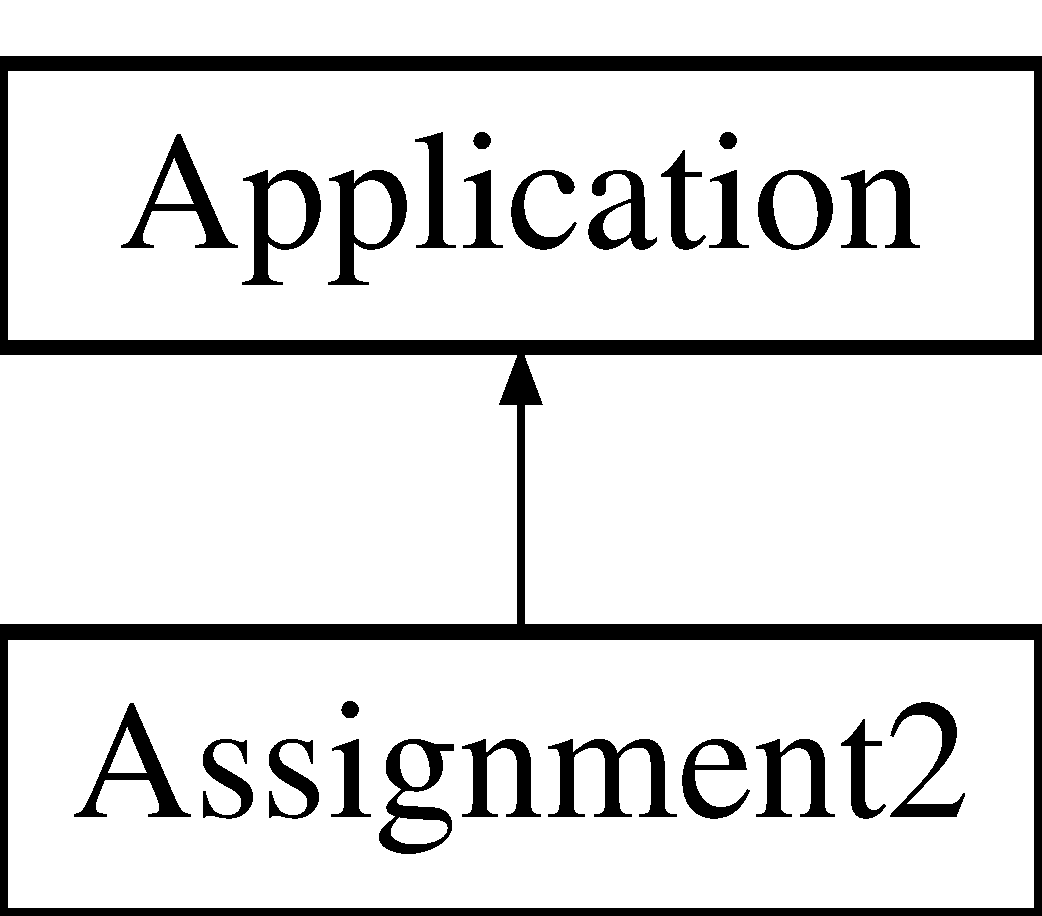
\includegraphics[height=2.000000cm]{class_assignment2}
\end{center}
\end{figure}
\subsection*{Public Member Functions}
\begin{DoxyCompactItemize}
\item
\hyperlink{class_assignment2_ac684d2ecb894a4e71f8359e3a2ebd37f}{Assignment2} (std\+::shared\+\_\+ptr$<$ class \hyperlink{class_scene}{Scene} $>$ input\+Scene, std\+::shared\+\_\+ptr$<$ class \hyperlink{class_camera}{Camera} $>$ input\+Camera)
\item
virtual glm\+::vec2 \hyperlink{class_assignment2_a9ea79bd468c12dde5159ca7b8efd8e1e}{Get\+Window\+Size} () const
\begin{DoxyCompactList}\small\item\em Specifies the initial window size. \end{DoxyCompactList}\item
virtual void \hyperlink{class_assignment2_a3ee099a8ba45db14103541981e3c4fe8}{Handle\+Input} (S\+D\+L\+\_\+\+Keysym key, Uint32 state, Uint8 repeat, double timestamp, double delta\+Time)
\begin{DoxyCompactList}\small\item\em Processes an S\+DL keyboard event which has type \href{https://wiki.libsdl.org/SDL_KeyboardEvent}{\tt S\+D\+L\+\_\+\+Keyboard\+Event}. \end{DoxyCompactList}\item
virtual void \hyperlink{class_assignment2_a41544ad361dd798d5fae1ec3197fc66e}{Tick} (double delta\+Time)
\begin{DoxyCompactList}\small\item\em Called every frame to advance program logic. \end{DoxyCompactList}\end{DoxyCompactItemize}
\subsection*{Static Public Member Functions}
\begin{DoxyCompactItemize}
\item
static std\+::unique\+\_\+ptr$<$ \hyperlink{class_application}{Application} $>$ \hyperlink{class_assignment2_ae4f0035275d5be2c053a598fbe3209e6}{Create\+Application} (std\+::shared\+\_\+ptr$<$ class \hyperlink{class_scene}{Scene} $>$ \hyperlink{class_application_a88c6615107a5094bb93fa5f153f79554}{scene}, std\+::shared\+\_\+ptr$<$ class \hyperlink{class_camera}{Camera} $>$ \hyperlink{class_application_a0e8589fcb13c520ba472473abe5a518d}{camera})
\item
static std\+::shared\+\_\+ptr$<$ class \hyperlink{class_camera}{Camera} $>$ \hyperlink{class_assignment2_a285e6d6ff330c03e28e49660ec178fa4}{Create\+Camera} ()
\end{DoxyCompactItemize}
\subsection*{Protected Member Functions}
\begin{DoxyCompactItemize}
\item
virtual void \hyperlink{class_assignment2_a1af734567de5e8e73a2fd726fe3914f2}{Handle\+Window\+Resize} (float x, float y)
\begin{DoxyCompactList}\small\item\em Called by \hyperlink{class_application_a74d92db64e051efa56d0357989dcb755}{Handle\+Window\+Event()} when the window is resized. \end{DoxyCompactList}\end{DoxyCompactItemize}
\subsection*{Private Member Functions}
\begin{DoxyCompactItemize}
\item
virtual void \hyperlink{class_assignment2_aa4f8ccd09a7accbdf093394c6ee4f63f}{Setup\+Scene} ()
\begin{DoxyCompactList}\small\item\em Called by \hyperlink{class_application_a17cf1ea4552d26a1c20f7d98d793d41d}{Initialize()} to populate the scene. \end{DoxyCompactList}\item
virtual void \hyperlink{class_assignment2_a2f42c6da59d8b5ba5dc4796d8bd13d30}{Setup\+Example1} ()
\item
virtual void \hyperlink{class_assignment2_aa26c3cd3e97be7ef88aae8d26d4af6bc}{Setup\+Example2} ()
\item
virtual void \hyperlink{class_assignment2_ab9ace1ffdac8f7425c64d661f3d13acd}{Setup\+Camera} ()
\begin{DoxyCompactList}\small\item\em Called by \hyperlink{class_application_a17cf1ea4552d26a1c20f7d98d793d41d}{Initialize()} to setup the camera. \end{DoxyCompactList}\end{DoxyCompactItemize}
\subsection*{Private Attributes}
\begin{DoxyCompactItemize}
\item
std\+::shared\+\_\+ptr$<$ class \hyperlink{class_scene_object}{Scene\+Object} $>$ \hyperlink{class_assignment2_a3afcc7cf71f0b1eb855482057beb1146}{scene\+Object}
\item
std\+::shared\+\_\+ptr$<$ class \hyperlink{class_light}{Light} $>$ \hyperlink{class_assignment2_abaf6127e0de097717673c0d9b04f8c79}{point\+Light}
\end{DoxyCompactItemize}
\subsection*{Additional Inherited Members}


\subsection{Constructor \& Destructor Documentation}
\hypertarget{class_assignment2_ac684d2ecb894a4e71f8359e3a2ebd37f}{}\label{class_assignment2_ac684d2ecb894a4e71f8359e3a2ebd37f}
\index{Assignment2@{Assignment2}!Assignment2@{Assignment2}}
\index{Assignment2@{Assignment2}!Assignment2@{Assignment2}}
\subsubsection{\texorpdfstring{Assignment2()}{Assignment2()}}
{\footnotesize\ttfamily Assignment2\+::\+Assignment2 (\begin{DoxyParamCaption}\item[{std\+::shared\+\_\+ptr$<$ class \hyperlink{class_scene}{Scene} $>$}]{input\+Scene,  }\item[{std\+::shared\+\_\+ptr$<$ class \hyperlink{class_camera}{Camera} $>$}]{input\+Camera }\end{DoxyParamCaption})}



\subsection{Member Function Documentation}
\hypertarget{class_assignment2_ae4f0035275d5be2c053a598fbe3209e6}{}\label{class_assignment2_ae4f0035275d5be2c053a598fbe3209e6}
\index{Assignment2@{Assignment2}!Create\+Application@{Create\+Application}}
\index{Create\+Application@{Create\+Application}!Assignment2@{Assignment2}}
\subsubsection{\texorpdfstring{Create\+Application()}{CreateApplication()}}
{\footnotesize\ttfamily std\+::unique\+\_\+ptr$<$ \hyperlink{class_application}{Application} $>$ Assignment2\+::\+Create\+Application (\begin{DoxyParamCaption}\item[{std\+::shared\+\_\+ptr$<$ class \hyperlink{class_scene}{Scene} $>$}]{scene,  }\item[{std\+::shared\+\_\+ptr$<$ class \hyperlink{class_camera}{Camera} $>$}]{camera }\end{DoxyParamCaption})\hspace{0.3cm}{\ttfamily [static]}}

\hypertarget{class_assignment2_a285e6d6ff330c03e28e49660ec178fa4}{}\label{class_assignment2_a285e6d6ff330c03e28e49660ec178fa4}
\index{Assignment2@{Assignment2}!Create\+Camera@{Create\+Camera}}
\index{Create\+Camera@{Create\+Camera}!Assignment2@{Assignment2}}
\subsubsection{\texorpdfstring{Create\+Camera()}{CreateCamera()}}
{\footnotesize\ttfamily std\+::shared\+\_\+ptr$<$ class \hyperlink{class_camera}{Camera} $>$ Assignment2\+::\+Create\+Camera (\begin{DoxyParamCaption}{ }\end{DoxyParamCaption})\hspace{0.3cm}{\ttfamily [static]}}

\hypertarget{class_assignment2_a9ea79bd468c12dde5159ca7b8efd8e1e}{}\label{class_assignment2_a9ea79bd468c12dde5159ca7b8efd8e1e}
\index{Assignment2@{Assignment2}!Get\+Window\+Size@{Get\+Window\+Size}}
\index{Get\+Window\+Size@{Get\+Window\+Size}!Assignment2@{Assignment2}}
\subsubsection{\texorpdfstring{Get\+Window\+Size()}{GetWindowSize()}}
{\footnotesize\ttfamily glm\+::vec2 Assignment2\+::\+Get\+Window\+Size (\begin{DoxyParamCaption}{ }\end{DoxyParamCaption}) const\hspace{0.3cm}{\ttfamily [virtual]}}



Specifies the initial window size.

\begin{DoxyReturn}{Returns}
The desired window size.
\end{DoxyReturn}


Reimplemented from \hyperlink{class_application_ab190ae0e987fe95682714dd4b2495e82}{Application}.

\hypertarget{class_assignment2_a3ee099a8ba45db14103541981e3c4fe8}{}\label{class_assignment2_a3ee099a8ba45db14103541981e3c4fe8}
\index{Assignment2@{Assignment2}!Handle\+Input@{Handle\+Input}}
\index{Handle\+Input@{Handle\+Input}!Assignment2@{Assignment2}}
\subsubsection{\texorpdfstring{Handle\+Input()}{HandleInput()}}
{\footnotesize\ttfamily void Assignment2\+::\+Handle\+Input (\begin{DoxyParamCaption}\item[{S\+D\+L\+\_\+\+Keysym}]{key,  }\item[{Uint32}]{state,  }\item[{Uint8}]{repeat,  }\item[{double}]{timestamp,  }\item[{double}]{delta\+Time }\end{DoxyParamCaption})\hspace{0.3cm}{\ttfamily [virtual]}}



Processes an S\+DL keyboard event which has type \href{https://wiki.libsdl.org/SDL_KeyboardEvent}{\tt S\+D\+L\+\_\+\+Keyboard\+Event}.


\begin{DoxyParams}{Parameters}
{\em key} & See the S\+DL documentation for more details about \href{https://wiki.libsdl.org/SDL_Keysym}{\tt S\+D\+L\+\_\+\+Keysym}. \\
\hline
{\em state} & This is the type field in the \href{https://wiki.libsdl.org/SDL_Event}{\tt S\+D\+L\+\_\+\+Event}datastructure. \\
\hline
{\em repeat} & This value is non-\/zero is the key is being repeated. \\
\hline
{\em timestamp} & Timestamp is the number of seconds since the program was first started. \\
\hline
{\em delta\+Time} & The amount of time (in seconds) since the last tick.\\
\hline
\end{DoxyParams}
Takes in a keyboard event and process it. This does nothing by default. \textquotesingle{}delta\+Time\textquotesingle{} is included to allow you to move something and have the movement look smooth. For example, if you have an object that you want to move forward whenever \textquotesingle{}W\textquotesingle{} is pressed. You know that the object travels at 10 meters per second when \textquotesingle{}W\textquotesingle{} is pressed and 0 meters per second when it is not. How far should you move the object? You would want to move it forward by $10 \cdot deltaTime $ units.

Reimplemented from \hyperlink{class_application_ae6074c3f102de1cb2fe4c81b545679db}{Application}.

\hypertarget{class_assignment2_a1af734567de5e8e73a2fd726fe3914f2}{}\label{class_assignment2_a1af734567de5e8e73a2fd726fe3914f2}
\index{Assignment2@{Assignment2}!Handle\+Window\+Resize@{Handle\+Window\+Resize}}
\index{Handle\+Window\+Resize@{Handle\+Window\+Resize}!Assignment2@{Assignment2}}
\subsubsection{\texorpdfstring{Handle\+Window\+Resize()}{HandleWindowResize()}}
{\footnotesize\ttfamily void Assignment2\+::\+Handle\+Window\+Resize (\begin{DoxyParamCaption}\item[{float}]{x,  }\item[{float}]{y }\end{DoxyParamCaption})\hspace{0.3cm}{\ttfamily [protected]}, {\ttfamily [virtual]}}



Called by \hyperlink{class_application_a74d92db64e051efa56d0357989dcb755}{Handle\+Window\+Event()} when the window is resized.


\begin{DoxyParams}{Parameters}
{\em x} & The width of the window. \\
\hline
{\em y} & The height of the window.\\
\hline
\end{DoxyParams}
By default calls, \href{https://www.opengl.org/sdk/docs/man/html/glViewport.xhtml}{\tt gl\+Viewport} to resize the viewport as necessary. If any part of your application depends on the window resize, you will want to take care of it in this function! (Hint for the O\+P\+T\+I\+O\+N\+AL deferred rendering task in assignment 2\+: your \textquotesingle{}G-\/\+Buffers\textquotesingle{} should be resized).

Reimplemented from \hyperlink{class_application_abdba284a0f075ee1d4a2108c3a5236a2}{Application}.

\hypertarget{class_assignment2_ab9ace1ffdac8f7425c64d661f3d13acd}{}\label{class_assignment2_ab9ace1ffdac8f7425c64d661f3d13acd}
\index{Assignment2@{Assignment2}!Setup\+Camera@{Setup\+Camera}}
\index{Setup\+Camera@{Setup\+Camera}!Assignment2@{Assignment2}}
\subsubsection{\texorpdfstring{Setup\+Camera()}{SetupCamera()}}
{\footnotesize\ttfamily void Assignment2\+::\+Setup\+Camera (\begin{DoxyParamCaption}{ }\end{DoxyParamCaption})\hspace{0.3cm}{\ttfamily [private]}, {\ttfamily [virtual]}}



Called by \hyperlink{class_application_a17cf1ea4552d26a1c20f7d98d793d41d}{Initialize()} to setup the camera.

Note by the time this function is called, the \hyperlink{class_application}{Application} sub-\/class is fully constructed and \hyperlink{class_camera}{Camera} object is already created.

Reimplemented from \hyperlink{class_application_a2eb61ca027f223a5c5ad1bf982481193}{Application}.

\hypertarget{class_assignment2_a2f42c6da59d8b5ba5dc4796d8bd13d30}{}\label{class_assignment2_a2f42c6da59d8b5ba5dc4796d8bd13d30}
\index{Assignment2@{Assignment2}!Setup\+Example1@{Setup\+Example1}}
\index{Setup\+Example1@{Setup\+Example1}!Assignment2@{Assignment2}}
\subsubsection{\texorpdfstring{Setup\+Example1()}{SetupExample1()}}
{\footnotesize\ttfamily void Assignment2\+::\+Setup\+Example1 (\begin{DoxyParamCaption}{ }\end{DoxyParamCaption})\hspace{0.3cm}{\ttfamily [private]}, {\ttfamily [virtual]}}

\hypertarget{class_assignment2_aa26c3cd3e97be7ef88aae8d26d4af6bc}{}\label{class_assignment2_aa26c3cd3e97be7ef88aae8d26d4af6bc}
\index{Assignment2@{Assignment2}!Setup\+Example2@{Setup\+Example2}}
\index{Setup\+Example2@{Setup\+Example2}!Assignment2@{Assignment2}}
\subsubsection{\texorpdfstring{Setup\+Example2()}{SetupExample2()}}
{\footnotesize\ttfamily void Assignment2\+::\+Setup\+Example2 (\begin{DoxyParamCaption}{ }\end{DoxyParamCaption})\hspace{0.3cm}{\ttfamily [private]}, {\ttfamily [virtual]}}

\hypertarget{class_assignment2_aa4f8ccd09a7accbdf093394c6ee4f63f}{}\label{class_assignment2_aa4f8ccd09a7accbdf093394c6ee4f63f}
\index{Assignment2@{Assignment2}!Setup\+Scene@{Setup\+Scene}}
\index{Setup\+Scene@{Setup\+Scene}!Assignment2@{Assignment2}}
\subsubsection{\texorpdfstring{Setup\+Scene()}{SetupScene()}}
{\footnotesize\ttfamily void Assignment2\+::\+Setup\+Scene (\begin{DoxyParamCaption}{ }\end{DoxyParamCaption})\hspace{0.3cm}{\ttfamily [private]}, {\ttfamily [virtual]}}



Called by \hyperlink{class_application_a17cf1ea4552d26a1c20f7d98d793d41d}{Initialize()} to populate the scene.

Note by the time this function is called, the \hyperlink{class_application}{Application} sub-\/class is fully constructed and \hyperlink{class_scene}{Scene} object is already created.

Reimplemented from \hyperlink{class_application_aa8e8017ef8dd86293c96d0645e66d440}{Application}.

\hypertarget{class_assignment2_a41544ad361dd798d5fae1ec3197fc66e}{}\label{class_assignment2_a41544ad361dd798d5fae1ec3197fc66e}
\index{Assignment2@{Assignment2}!Tick@{Tick}}
\index{Tick@{Tick}!Assignment2@{Assignment2}}
\subsubsection{\texorpdfstring{Tick()}{Tick()}}
{\footnotesize\ttfamily void Assignment2\+::\+Tick (\begin{DoxyParamCaption}\item[{double}]{delta\+Time }\end{DoxyParamCaption})\hspace{0.3cm}{\ttfamily [virtual]}}



Called every frame to advance program logic.


\begin{DoxyParams}{Parameters}
{\em delta\+Time} & The amount of time (in seconds) since the last tick.\\
\hline
\end{DoxyParams}
If you need something in the \hyperlink{class_scene}{Scene} to change over time, this is where you should implement that logic. It is recommended that you make use of the delta\+Time variable to make things change smoothly!

Reimplemented from \hyperlink{class_application_a0800afd5651153d31fa775a8048d14dd}{Application}.



\subsection{Member Data Documentation}
\hypertarget{class_assignment2_abaf6127e0de097717673c0d9b04f8c79}{}\label{class_assignment2_abaf6127e0de097717673c0d9b04f8c79}
\index{Assignment2@{Assignment2}!point\+Light@{point\+Light}}
\index{point\+Light@{point\+Light}!Assignment2@{Assignment2}}
\subsubsection{\texorpdfstring{point\+Light}{pointLight}}
{\footnotesize\ttfamily std\+::shared\+\_\+ptr$<$class \hyperlink{class_light}{Light}$>$ Assignment2\+::point\+Light\hspace{0.3cm}{\ttfamily [private]}}

\hypertarget{class_assignment2_a3afcc7cf71f0b1eb855482057beb1146}{}\label{class_assignment2_a3afcc7cf71f0b1eb855482057beb1146}
\index{Assignment2@{Assignment2}!scene\+Object@{scene\+Object}}
\index{scene\+Object@{scene\+Object}!Assignment2@{Assignment2}}
\subsubsection{\texorpdfstring{scene\+Object}{sceneObject}}
{\footnotesize\ttfamily std\+::shared\+\_\+ptr$<$class \hyperlink{class_scene_object}{Scene\+Object}$>$ Assignment2\+::scene\+Object\hspace{0.3cm}{\ttfamily [private]}}



The documentation for this class was generated from the following files\+:\begin{DoxyCompactItemize}
\item
/data/MO814A-MC937A/MO814A-MC937Aopengl-\/instructor/source/assignment2/\hyperlink{_assignment2_8h}{Assignment2.\+h}\item
/data/MO814A-MC937A/MO814A-MC937Aopengl-\/instructor/source/assignment2/\hyperlink{_assignment2_8cpp}{Assignment2.\+cpp}\end{DoxyCompactItemize}

\hypertarget{class_assignment3}{}\section{Assignment3 Class Reference}
\label{class_assignment3}\index{Assignment3@{Assignment3}}


{\ttfamily \#include $<$Assignment3.\+h$>$}

Inheritance diagram for Assignment3\+:\begin{figure}[H]
\begin{center}
\leavevmode
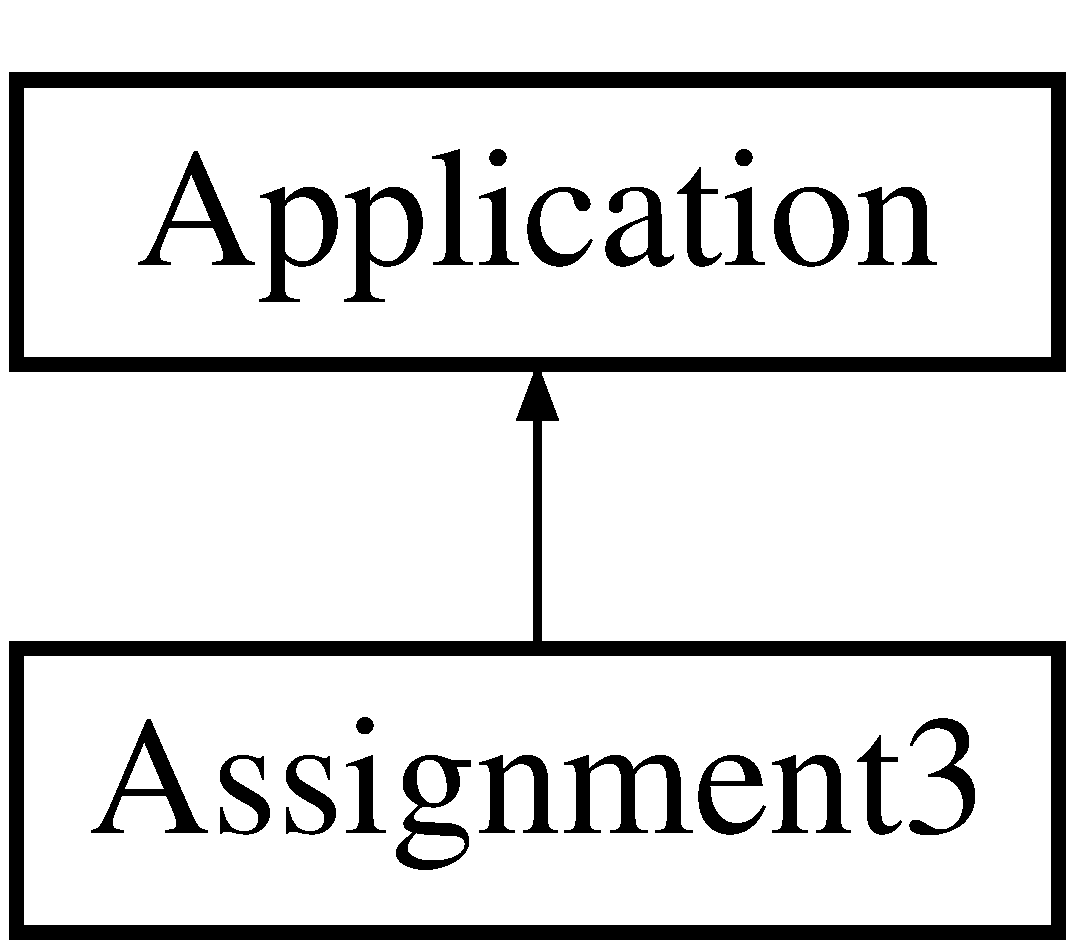
\includegraphics[height=2.000000cm]{class_assignment3}
\end{center}
\end{figure}
\subsection*{Public Member Functions}
\begin{DoxyCompactItemize}
\item
\hyperlink{class_assignment3_adb8e9ac0681c600affc3370f5e5422b2}{Assignment3} (std\+::shared\+\_\+ptr$<$ class \hyperlink{class_scene}{Scene} $>$ input\+Scene, std\+::shared\+\_\+ptr$<$ class \hyperlink{class_camera}{Camera} $>$ input\+Camera)
\item
virtual glm\+::vec2 \hyperlink{class_assignment3_aec48ba5500d906963fdac555ee47cb72}{Get\+Window\+Size} () const
\begin{DoxyCompactList}\small\item\em Specifies the initial window size. \end{DoxyCompactList}\item
virtual void \hyperlink{class_assignment3_a1cc65ca321f39eb7092959b2dada8d31}{Handle\+Input} (S\+D\+L\+\_\+\+Keysym key, Uint32 state, Uint8 repeat, double timestamp, double delta\+Time)
\begin{DoxyCompactList}\small\item\em Processes an S\+DL keyboard event which has type \href{https://wiki.libsdl.org/SDL_KeyboardEvent}{\tt S\+D\+L\+\_\+\+Keyboard\+Event}. \end{DoxyCompactList}\item
virtual void \hyperlink{class_assignment3_a11256b6e7b38ab24baa92729cfb8ffe2}{Tick} (double delta\+Time)
\begin{DoxyCompactList}\small\item\em Called every frame to advance program logic. \end{DoxyCompactList}\end{DoxyCompactItemize}
\subsection*{Static Public Member Functions}
\begin{DoxyCompactItemize}
\item
static std\+::unique\+\_\+ptr$<$ \hyperlink{class_application}{Application} $>$ \hyperlink{class_assignment3_a12b30bd7b8a0bcefbd977f126ce00b25}{Create\+Application} (std\+::shared\+\_\+ptr$<$ class \hyperlink{class_scene}{Scene} $>$ \hyperlink{class_application_a88c6615107a5094bb93fa5f153f79554}{scene}, std\+::shared\+\_\+ptr$<$ class \hyperlink{class_camera}{Camera} $>$ \hyperlink{class_application_a0e8589fcb13c520ba472473abe5a518d}{camera})
\item
static std\+::shared\+\_\+ptr$<$ class \hyperlink{class_camera}{Camera} $>$ \hyperlink{class_assignment3_a47d1b58079eee3e135e08768cd2a2461}{Create\+Camera} ()
\end{DoxyCompactItemize}
\subsection*{Protected Member Functions}
\begin{DoxyCompactItemize}
\item
virtual void \hyperlink{class_assignment3_a851c637c83c8092d8adfb5c9f761daeb}{Handle\+Window\+Resize} (float x, float y)
\begin{DoxyCompactList}\small\item\em Called by \hyperlink{class_application_a74d92db64e051efa56d0357989dcb755}{Handle\+Window\+Event()} when the window is resized. \end{DoxyCompactList}\end{DoxyCompactItemize}
\subsection*{Private Member Functions}
\begin{DoxyCompactItemize}
\item
virtual void \hyperlink{class_assignment3_a2dc29d9016a9d822ede84b9ef41429a5}{Setup\+Scene} ()
\begin{DoxyCompactList}\small\item\em Called by \hyperlink{class_application_a17cf1ea4552d26a1c20f7d98d793d41d}{Initialize()} to populate the scene. \end{DoxyCompactList}\item
virtual void \hyperlink{class_assignment3_a468c30083d6f75d99cd1fe41205983dc}{Setup\+Example1} ()
\item
virtual void \hyperlink{class_assignment3_af6d27b156c0781ff6aba450bd78b61ff}{Setup\+Example2} ()
\item
virtual void \hyperlink{class_assignment3_a1d23eb19973b78e516169f4a03954526}{Setup\+Camera} ()
\begin{DoxyCompactList}\small\item\em Called by \hyperlink{class_application_a17cf1ea4552d26a1c20f7d98d793d41d}{Initialize()} to setup the camera. \end{DoxyCompactList}\end{DoxyCompactItemize}
\subsection*{Private Attributes}
\begin{DoxyCompactItemize}
\item
std\+::shared\+\_\+ptr$<$ class \hyperlink{class_scene_object}{Scene\+Object} $>$ \hyperlink{class_assignment3_a0bc175d3efff30c5f4aa3ffa1272338a}{scene\+Object}
\item
std\+::shared\+\_\+ptr$<$ class \hyperlink{class_light}{Light} $>$ \hyperlink{class_assignment3_ad1cf5a76d62b5a1ed17e66c31e0feb98}{point\+Light}
\end{DoxyCompactItemize}
\subsection*{Additional Inherited Members}


\subsection{Constructor \& Destructor Documentation}
\hypertarget{class_assignment3_adb8e9ac0681c600affc3370f5e5422b2}{}\label{class_assignment3_adb8e9ac0681c600affc3370f5e5422b2}
\index{Assignment3@{Assignment3}!Assignment3@{Assignment3}}
\index{Assignment3@{Assignment3}!Assignment3@{Assignment3}}
\subsubsection{\texorpdfstring{Assignment3()}{Assignment3()}}
{\footnotesize\ttfamily Assignment3\+::\+Assignment3 (\begin{DoxyParamCaption}\item[{std\+::shared\+\_\+ptr$<$ class \hyperlink{class_scene}{Scene} $>$}]{input\+Scene,  }\item[{std\+::shared\+\_\+ptr$<$ class \hyperlink{class_camera}{Camera} $>$}]{input\+Camera }\end{DoxyParamCaption})}



\subsection{Member Function Documentation}
\hypertarget{class_assignment3_a12b30bd7b8a0bcefbd977f126ce00b25}{}\label{class_assignment3_a12b30bd7b8a0bcefbd977f126ce00b25}
\index{Assignment3@{Assignment3}!Create\+Application@{Create\+Application}}
\index{Create\+Application@{Create\+Application}!Assignment3@{Assignment3}}
\subsubsection{\texorpdfstring{Create\+Application()}{CreateApplication()}}
{\footnotesize\ttfamily std\+::unique\+\_\+ptr$<$ \hyperlink{class_application}{Application} $>$ Assignment3\+::\+Create\+Application (\begin{DoxyParamCaption}\item[{std\+::shared\+\_\+ptr$<$ class \hyperlink{class_scene}{Scene} $>$}]{scene,  }\item[{std\+::shared\+\_\+ptr$<$ class \hyperlink{class_camera}{Camera} $>$}]{camera }\end{DoxyParamCaption})\hspace{0.3cm}{\ttfamily [static]}}

\hypertarget{class_assignment3_a47d1b58079eee3e135e08768cd2a2461}{}\label{class_assignment3_a47d1b58079eee3e135e08768cd2a2461}
\index{Assignment3@{Assignment3}!Create\+Camera@{Create\+Camera}}
\index{Create\+Camera@{Create\+Camera}!Assignment3@{Assignment3}}
\subsubsection{\texorpdfstring{Create\+Camera()}{CreateCamera()}}
{\footnotesize\ttfamily std\+::shared\+\_\+ptr$<$ class \hyperlink{class_camera}{Camera} $>$ Assignment3\+::\+Create\+Camera (\begin{DoxyParamCaption}{ }\end{DoxyParamCaption})\hspace{0.3cm}{\ttfamily [static]}}

\hypertarget{class_assignment3_aec48ba5500d906963fdac555ee47cb72}{}\label{class_assignment3_aec48ba5500d906963fdac555ee47cb72}
\index{Assignment3@{Assignment3}!Get\+Window\+Size@{Get\+Window\+Size}}
\index{Get\+Window\+Size@{Get\+Window\+Size}!Assignment3@{Assignment3}}
\subsubsection{\texorpdfstring{Get\+Window\+Size()}{GetWindowSize()}}
{\footnotesize\ttfamily glm\+::vec2 Assignment3\+::\+Get\+Window\+Size (\begin{DoxyParamCaption}{ }\end{DoxyParamCaption}) const\hspace{0.3cm}{\ttfamily [virtual]}}



Specifies the initial window size.

\begin{DoxyReturn}{Returns}
The desired window size.
\end{DoxyReturn}


Reimplemented from \hyperlink{class_application_ab190ae0e987fe95682714dd4b2495e82}{Application}.

\hypertarget{class_assignment3_a1cc65ca321f39eb7092959b2dada8d31}{}\label{class_assignment3_a1cc65ca321f39eb7092959b2dada8d31}
\index{Assignment3@{Assignment3}!Handle\+Input@{Handle\+Input}}
\index{Handle\+Input@{Handle\+Input}!Assignment3@{Assignment3}}
\subsubsection{\texorpdfstring{Handle\+Input()}{HandleInput()}}
{\footnotesize\ttfamily void Assignment3\+::\+Handle\+Input (\begin{DoxyParamCaption}\item[{S\+D\+L\+\_\+\+Keysym}]{key,  }\item[{Uint32}]{state,  }\item[{Uint8}]{repeat,  }\item[{double}]{timestamp,  }\item[{double}]{delta\+Time }\end{DoxyParamCaption})\hspace{0.3cm}{\ttfamily [virtual]}}



Processes an S\+DL keyboard event which has type \href{https://wiki.libsdl.org/SDL_KeyboardEvent}{\tt S\+D\+L\+\_\+\+Keyboard\+Event}.


\begin{DoxyParams}{Parameters}
{\em key} & See the S\+DL documentation for more details about \href{https://wiki.libsdl.org/SDL_Keysym}{\tt S\+D\+L\+\_\+\+Keysym}. \\
\hline
{\em state} & This is the type field in the \href{https://wiki.libsdl.org/SDL_Event}{\tt S\+D\+L\+\_\+\+Event}datastructure. \\
\hline
{\em repeat} & This value is non-\/zero is the key is being repeated. \\
\hline
{\em timestamp} & Timestamp is the number of seconds since the program was first started. \\
\hline
{\em delta\+Time} & The amount of time (in seconds) since the last tick.\\
\hline
\end{DoxyParams}
Takes in a keyboard event and process it. This does nothing by default. \textquotesingle{}delta\+Time\textquotesingle{} is included to allow you to move something and have the movement look smooth. For example, if you have an object that you want to move forward whenever \textquotesingle{}W\textquotesingle{} is pressed. You know that the object travels at 10 meters per second when \textquotesingle{}W\textquotesingle{} is pressed and 0 meters per second when it is not. How far should you move the object? You would want to move it forward by $10 \cdot deltaTime $ units.

Reimplemented from \hyperlink{class_application_ae6074c3f102de1cb2fe4c81b545679db}{Application}.

\hypertarget{class_assignment3_a851c637c83c8092d8adfb5c9f761daeb}{}\label{class_assignment3_a851c637c83c8092d8adfb5c9f761daeb}
\index{Assignment3@{Assignment3}!Handle\+Window\+Resize@{Handle\+Window\+Resize}}
\index{Handle\+Window\+Resize@{Handle\+Window\+Resize}!Assignment3@{Assignment3}}
\subsubsection{\texorpdfstring{Handle\+Window\+Resize()}{HandleWindowResize()}}
{\footnotesize\ttfamily void Assignment3\+::\+Handle\+Window\+Resize (\begin{DoxyParamCaption}\item[{float}]{x,  }\item[{float}]{y }\end{DoxyParamCaption})\hspace{0.3cm}{\ttfamily [protected]}, {\ttfamily [virtual]}}



Called by \hyperlink{class_application_a74d92db64e051efa56d0357989dcb755}{Handle\+Window\+Event()} when the window is resized.


\begin{DoxyParams}{Parameters}
{\em x} & The width of the window. \\
\hline
{\em y} & The height of the window.\\
\hline
\end{DoxyParams}
By default calls, \href{https://www.opengl.org/sdk/docs/man/html/glViewport.xhtml}{\tt gl\+Viewport} to resize the viewport as necessary. If any part of your application depends on the window resize, you will want to take care of it in this function! (Hint for the O\+P\+T\+I\+O\+N\+AL deferred rendering task in assignment 2\+: your \textquotesingle{}G-\/\+Buffers\textquotesingle{} should be resized).

Reimplemented from \hyperlink{class_application_abdba284a0f075ee1d4a2108c3a5236a2}{Application}.

\hypertarget{class_assignment3_a1d23eb19973b78e516169f4a03954526}{}\label{class_assignment3_a1d23eb19973b78e516169f4a03954526}
\index{Assignment3@{Assignment3}!Setup\+Camera@{Setup\+Camera}}
\index{Setup\+Camera@{Setup\+Camera}!Assignment3@{Assignment3}}
\subsubsection{\texorpdfstring{Setup\+Camera()}{SetupCamera()}}
{\footnotesize\ttfamily void Assignment3\+::\+Setup\+Camera (\begin{DoxyParamCaption}{ }\end{DoxyParamCaption})\hspace{0.3cm}{\ttfamily [private]}, {\ttfamily [virtual]}}



Called by \hyperlink{class_application_a17cf1ea4552d26a1c20f7d98d793d41d}{Initialize()} to setup the camera.

Note by the time this function is called, the \hyperlink{class_application}{Application} sub-\/class is fully constructed and \hyperlink{class_camera}{Camera} object is already created.

Reimplemented from \hyperlink{class_application_a2eb61ca027f223a5c5ad1bf982481193}{Application}.

\hypertarget{class_assignment3_a468c30083d6f75d99cd1fe41205983dc}{}\label{class_assignment3_a468c30083d6f75d99cd1fe41205983dc}
\index{Assignment3@{Assignment3}!Setup\+Example1@{Setup\+Example1}}
\index{Setup\+Example1@{Setup\+Example1}!Assignment3@{Assignment3}}
\subsubsection{\texorpdfstring{Setup\+Example1()}{SetupExample1()}}
{\footnotesize\ttfamily void Assignment3\+::\+Setup\+Example1 (\begin{DoxyParamCaption}{ }\end{DoxyParamCaption})\hspace{0.3cm}{\ttfamily [private]}, {\ttfamily [virtual]}}

\hypertarget{class_assignment3_af6d27b156c0781ff6aba450bd78b61ff}{}\label{class_assignment3_af6d27b156c0781ff6aba450bd78b61ff}
\index{Assignment3@{Assignment3}!Setup\+Example2@{Setup\+Example2}}
\index{Setup\+Example2@{Setup\+Example2}!Assignment3@{Assignment3}}
\subsubsection{\texorpdfstring{Setup\+Example2()}{SetupExample2()}}
{\footnotesize\ttfamily void Assignment3\+::\+Setup\+Example2 (\begin{DoxyParamCaption}{ }\end{DoxyParamCaption})\hspace{0.3cm}{\ttfamily [private]}, {\ttfamily [virtual]}}

\hypertarget{class_assignment3_a2dc29d9016a9d822ede84b9ef41429a5}{}\label{class_assignment3_a2dc29d9016a9d822ede84b9ef41429a5}
\index{Assignment3@{Assignment3}!Setup\+Scene@{Setup\+Scene}}
\index{Setup\+Scene@{Setup\+Scene}!Assignment3@{Assignment3}}
\subsubsection{\texorpdfstring{Setup\+Scene()}{SetupScene()}}
{\footnotesize\ttfamily void Assignment3\+::\+Setup\+Scene (\begin{DoxyParamCaption}{ }\end{DoxyParamCaption})\hspace{0.3cm}{\ttfamily [private]}, {\ttfamily [virtual]}}



Called by \hyperlink{class_application_a17cf1ea4552d26a1c20f7d98d793d41d}{Initialize()} to populate the scene.

Note by the time this function is called, the \hyperlink{class_application}{Application} sub-\/class is fully constructed and \hyperlink{class_scene}{Scene} object is already created.

Reimplemented from \hyperlink{class_application_aa8e8017ef8dd86293c96d0645e66d440}{Application}.

\hypertarget{class_assignment3_a11256b6e7b38ab24baa92729cfb8ffe2}{}\label{class_assignment3_a11256b6e7b38ab24baa92729cfb8ffe2}
\index{Assignment3@{Assignment3}!Tick@{Tick}}
\index{Tick@{Tick}!Assignment3@{Assignment3}}
\subsubsection{\texorpdfstring{Tick()}{Tick()}}
{\footnotesize\ttfamily void Assignment3\+::\+Tick (\begin{DoxyParamCaption}\item[{double}]{delta\+Time }\end{DoxyParamCaption})\hspace{0.3cm}{\ttfamily [virtual]}}



Called every frame to advance program logic.


\begin{DoxyParams}{Parameters}
{\em delta\+Time} & The amount of time (in seconds) since the last tick.\\
\hline
\end{DoxyParams}
If you need something in the \hyperlink{class_scene}{Scene} to change over time, this is where you should implement that logic. It is recommended that you make use of the delta\+Time variable to make things change smoothly!

Reimplemented from \hyperlink{class_application_a0800afd5651153d31fa775a8048d14dd}{Application}.



\subsection{Member Data Documentation}
\hypertarget{class_assignment3_ad1cf5a76d62b5a1ed17e66c31e0feb98}{}\label{class_assignment3_ad1cf5a76d62b5a1ed17e66c31e0feb98}
\index{Assignment3@{Assignment3}!point\+Light@{point\+Light}}
\index{point\+Light@{point\+Light}!Assignment3@{Assignment3}}
\subsubsection{\texorpdfstring{point\+Light}{pointLight}}
{\footnotesize\ttfamily std\+::shared\+\_\+ptr$<$class \hyperlink{class_light}{Light}$>$ Assignment3\+::point\+Light\hspace{0.3cm}{\ttfamily [private]}}

\hypertarget{class_assignment3_a0bc175d3efff30c5f4aa3ffa1272338a}{}\label{class_assignment3_a0bc175d3efff30c5f4aa3ffa1272338a}
\index{Assignment3@{Assignment3}!scene\+Object@{scene\+Object}}
\index{scene\+Object@{scene\+Object}!Assignment3@{Assignment3}}
\subsubsection{\texorpdfstring{scene\+Object}{sceneObject}}
{\footnotesize\ttfamily std\+::shared\+\_\+ptr$<$class \hyperlink{class_scene_object}{Scene\+Object}$>$ Assignment3\+::scene\+Object\hspace{0.3cm}{\ttfamily [private]}}



The documentation for this class was generated from the following files\+:\begin{DoxyCompactItemize}
\item
/data/MO814A-MC937A/MO814A-MC937Aopengl-\/instructor/source/assignment3/\hyperlink{_assignment3_8h}{Assignment3.\+h}\item
/data/MO814A-MC937A/MO814A-MC937Aopengl-\/instructor/source/assignment3/\hyperlink{_assignment3_8cpp}{Assignment3.\+cpp}\end{DoxyCompactItemize}

\hypertarget{class_assignment4}{}\section{Assignment4 Class Reference}
\label{class_assignment4}\index{Assignment4@{Assignment4}}


{\ttfamily \#include $<$Assignment4.\+h$>$}

Inheritance diagram for Assignment4\+:\begin{figure}[H]
\begin{center}
\leavevmode
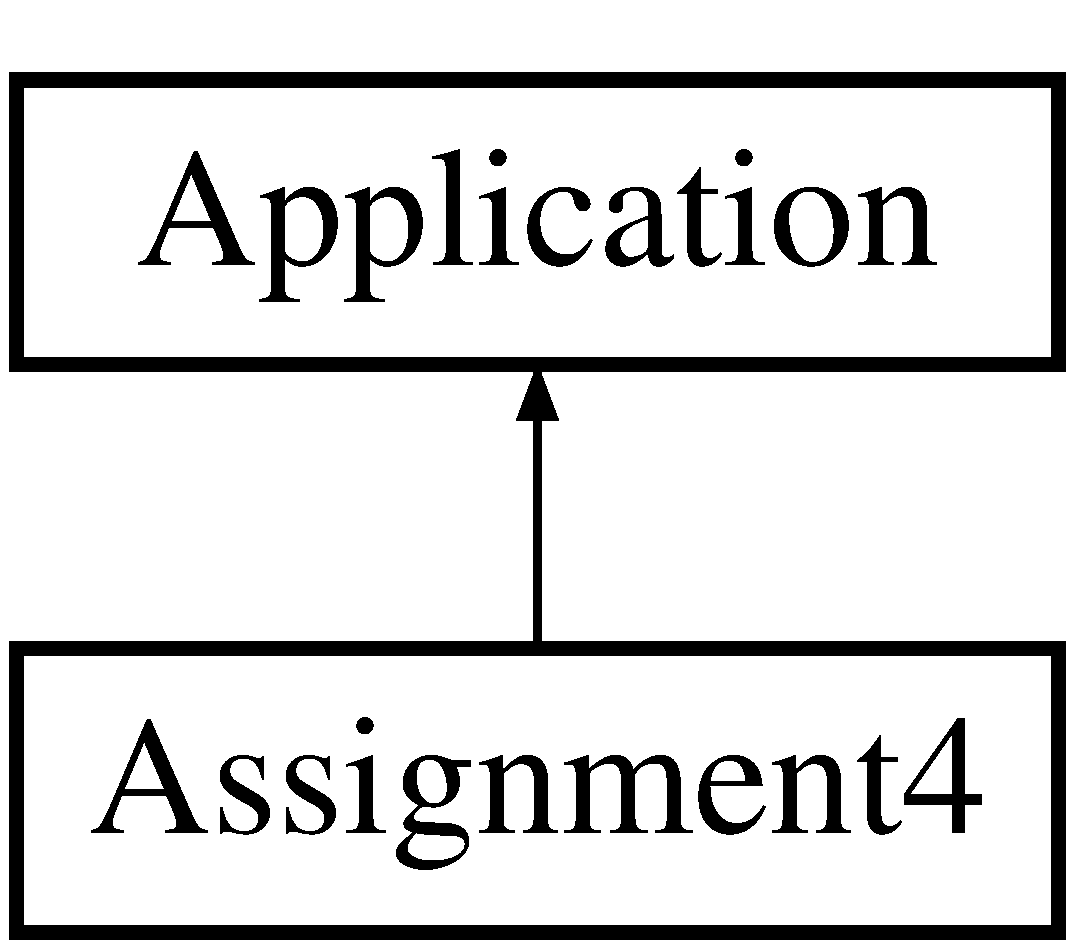
\includegraphics[height=2.000000cm]{class_assignment4}
\end{center}
\end{figure}
\subsection*{Public Member Functions}
\begin{DoxyCompactItemize}
\item
\hyperlink{class_assignment4_a318b02cf93165113069f3b44a8d13589}{Assignment4} (std\+::shared\+\_\+ptr$<$ class \hyperlink{class_scene}{Scene} $>$ input\+Scene, std\+::shared\+\_\+ptr$<$ class \hyperlink{class_camera}{Camera} $>$ input\+Camera)
\item 
virtual glm\+::vec2 \hyperlink{class_assignment4_ad197b75e730f9b32458429df8d55458e}{Get\+Window\+Size} () const
\begin{DoxyCompactList}\small\item\em Specifies the initial window size. \end{DoxyCompactList}\item
virtual void \hyperlink{class_assignment4_a02c51d46e2cbb55e7963b6bfbedaf1c4}{Handle\+Input} (S\+D\+L\+\_\+\+Keysym key, Uint32 state, Uint8 repeat, double timestamp, double delta\+Time)
\begin{DoxyCompactList}\small\item\em Processes an S\+DL keyboard event which has type \href{https://wiki.libsdl.org/SDL_KeyboardEvent}{\tt S\+D\+L\+\_\+\+Keyboard\+Event}. \end{DoxyCompactList}\item
virtual void \hyperlink{class_assignment4_a3ef3fef7a6ae13603bc453b29e079c5d}{Tick} (double delta\+Time)
\begin{DoxyCompactList}\small\item\em Called every frame to advance program logic. \end{DoxyCompactList}\end{DoxyCompactItemize}
\subsection*{Static Public Member Functions}
\begin{DoxyCompactItemize}
\item
static std\+::unique\+\_\+ptr$<$ \hyperlink{class_application}{Application} $>$ \hyperlink{class_assignment4_a7a2d272e1ce394cd4e7b66e840c2c806}{Create\+Application} (std\+::shared\+\_\+ptr$<$ class \hyperlink{class_scene}{Scene} $>$ \hyperlink{class_application_a88c6615107a5094bb93fa5f153f79554}{scene}, std\+::shared\+\_\+ptr$<$ class \hyperlink{class_camera}{Camera} $>$ \hyperlink{class_application_a0e8589fcb13c520ba472473abe5a518d}{camera})
\item
static std\+::shared\+\_\+ptr$<$ class \hyperlink{class_camera}{Camera} $>$ \hyperlink{class_assignment4_af75a5deee12f42e4efac2c8857c7eb05}{Create\+Camera} ()
\end{DoxyCompactItemize}
\subsection*{Protected Member Functions}
\begin{DoxyCompactItemize}
\item
virtual void \hyperlink{class_assignment4_ac79558272dc476db3ee4a99793f401f2}{Handle\+Window\+Resize} (float x, float y)
\begin{DoxyCompactList}\small\item\em Called by \hyperlink{class_application_a74d92db64e051efa56d0357989dcb755}{Handle\+Window\+Event()} when the window is resized. \end{DoxyCompactList}\end{DoxyCompactItemize}
\subsection*{Private Member Functions}
\begin{DoxyCompactItemize}
\item
virtual void \hyperlink{class_assignment4_a38c50647bb65ff03aaf293fcc21dc5fd}{Setup\+Scene} ()
\begin{DoxyCompactList}\small\item\em Called by \hyperlink{class_application_a17cf1ea4552d26a1c20f7d98d793d41d}{Initialize()} to populate the scene. \end{DoxyCompactList}\item
virtual void \hyperlink{class_assignment4_a019c1cc10bd21a91a88e68e11f86b846}{Setup\+Example1} ()
\item
virtual void \hyperlink{class_assignment4_a440d520fc872a49fade29aa1eb7643d0}{Generic\+Setup\+Example} (std\+::shared\+\_\+ptr$<$ class \hyperlink{class_shader_program}{Shader\+Program} $>$ shader, std\+::shared\+\_\+ptr$<$ \hyperlink{class_shader_program}{Shader\+Program} $>$ ground\+Shader)
\item
virtual void \hyperlink{class_assignment4_aa2bc15adb48cf54e477fce0c686cf2f0}{Setup\+Camera} ()
\begin{DoxyCompactList}\small\item\em Called by \hyperlink{class_application_a17cf1ea4552d26a1c20f7d98d793d41d}{Initialize()} to setup the camera. \end{DoxyCompactList}\end{DoxyCompactItemize}
\subsection*{Private Attributes}
\begin{DoxyCompactItemize}
\item
std\+::shared\+\_\+ptr$<$ class \hyperlink{class_light}{Light} $>$ \hyperlink{class_assignment4_ab2981232ba58193de1682308a1dbafdc}{sun\+Light}
\item
std\+::shared\+\_\+ptr$<$ class \hyperlink{class_light}{Light} $>$ \hyperlink{class_assignment4_a2ea813219380cc65ef89749586f5d4b5}{hemisphere\+Light}
\item
std\+::shared\+\_\+ptr$<$ class \hyperlink{class_light}{Light} $>$ \hyperlink{class_assignment4_a327ee7158090e2a2db8763df3cb8608d}{point\+Light}
\item
std\+::vector$<$ std\+::shared\+\_\+ptr$<$ class \hyperlink{class_scene_object}{Scene\+Object} $>$ $>$ \hyperlink{class_assignment4_aa16802895aa2aef461d130479c81a015}{sphere\+Dance}
\end{DoxyCompactItemize}
\subsection*{Additional Inherited Members}


\subsection{Constructor \& Destructor Documentation}
\hypertarget{class_assignment4_a318b02cf93165113069f3b44a8d13589}{}\label{class_assignment4_a318b02cf93165113069f3b44a8d13589}
\index{Assignment4@{Assignment4}!Assignment4@{Assignment4}}
\index{Assignment4@{Assignment4}!Assignment4@{Assignment4}}
\subsubsection{\texorpdfstring{Assignment4()}{Assignment4()}}
{\footnotesize\ttfamily Assignment4\+::\+Assignment4 (\begin{DoxyParamCaption}\item[{std\+::shared\+\_\+ptr$<$ class \hyperlink{class_scene}{Scene} $>$}]{input\+Scene,  }\item[{std\+::shared\+\_\+ptr$<$ class \hyperlink{class_camera}{Camera} $>$}]{input\+Camera }\end{DoxyParamCaption})}



\subsection{Member Function Documentation}
\hypertarget{class_assignment4_a7a2d272e1ce394cd4e7b66e840c2c806}{}\label{class_assignment4_a7a2d272e1ce394cd4e7b66e840c2c806}
\index{Assignment4@{Assignment4}!Create\+Application@{Create\+Application}}
\index{Create\+Application@{Create\+Application}!Assignment4@{Assignment4}}
\subsubsection{\texorpdfstring{Create\+Application()}{CreateApplication()}}
{\footnotesize\ttfamily std\+::unique\+\_\+ptr$<$ \hyperlink{class_application}{Application} $>$ Assignment4\+::\+Create\+Application (\begin{DoxyParamCaption}\item[{std\+::shared\+\_\+ptr$<$ class \hyperlink{class_scene}{Scene} $>$}]{scene,  }\item[{std\+::shared\+\_\+ptr$<$ class \hyperlink{class_camera}{Camera} $>$}]{camera }\end{DoxyParamCaption})\hspace{0.3cm}{\ttfamily [static]}}

\hypertarget{class_assignment4_af75a5deee12f42e4efac2c8857c7eb05}{}\label{class_assignment4_af75a5deee12f42e4efac2c8857c7eb05}
\index{Assignment4@{Assignment4}!Create\+Camera@{Create\+Camera}}
\index{Create\+Camera@{Create\+Camera}!Assignment4@{Assignment4}}
\subsubsection{\texorpdfstring{Create\+Camera()}{CreateCamera()}}
{\footnotesize\ttfamily std\+::shared\+\_\+ptr$<$ class \hyperlink{class_camera}{Camera} $>$ Assignment4\+::\+Create\+Camera (\begin{DoxyParamCaption}{ }\end{DoxyParamCaption})\hspace{0.3cm}{\ttfamily [static]}}

\hypertarget{class_assignment4_a440d520fc872a49fade29aa1eb7643d0}{}\label{class_assignment4_a440d520fc872a49fade29aa1eb7643d0}
\index{Assignment4@{Assignment4}!Generic\+Setup\+Example@{Generic\+Setup\+Example}}
\index{Generic\+Setup\+Example@{Generic\+Setup\+Example}!Assignment4@{Assignment4}}
\subsubsection{\texorpdfstring{Generic\+Setup\+Example()}{GenericSetupExample()}}
{\footnotesize\ttfamily void Assignment4\+::\+Generic\+Setup\+Example (\begin{DoxyParamCaption}\item[{std\+::shared\+\_\+ptr$<$ class \hyperlink{class_shader_program}{Shader\+Program} $>$}]{shader,  }\item[{std\+::shared\+\_\+ptr$<$ \hyperlink{class_shader_program}{Shader\+Program} $>$}]{ground\+Shader }\end{DoxyParamCaption})\hspace{0.3cm}{\ttfamily [private]}, {\ttfamily [virtual]}}

\hypertarget{class_assignment4_ad197b75e730f9b32458429df8d55458e}{}\label{class_assignment4_ad197b75e730f9b32458429df8d55458e}
\index{Assignment4@{Assignment4}!Get\+Window\+Size@{Get\+Window\+Size}}
\index{Get\+Window\+Size@{Get\+Window\+Size}!Assignment4@{Assignment4}}
\subsubsection{\texorpdfstring{Get\+Window\+Size()}{GetWindowSize()}}
{\footnotesize\ttfamily glm\+::vec2 Assignment4\+::\+Get\+Window\+Size (\begin{DoxyParamCaption}{ }\end{DoxyParamCaption}) const\hspace{0.3cm}{\ttfamily [virtual]}}



Specifies the initial window size.

\begin{DoxyReturn}{Returns}
The desired window size.
\end{DoxyReturn}


Reimplemented from \hyperlink{class_application_ab190ae0e987fe95682714dd4b2495e82}{Application}.

\hypertarget{class_assignment4_a02c51d46e2cbb55e7963b6bfbedaf1c4}{}\label{class_assignment4_a02c51d46e2cbb55e7963b6bfbedaf1c4}
\index{Assignment4@{Assignment4}!Handle\+Input@{Handle\+Input}}
\index{Handle\+Input@{Handle\+Input}!Assignment4@{Assignment4}}
\subsubsection{\texorpdfstring{Handle\+Input()}{HandleInput()}}
{\footnotesize\ttfamily void Assignment4\+::\+Handle\+Input (\begin{DoxyParamCaption}\item[{S\+D\+L\+\_\+\+Keysym}]{key,  }\item[{Uint32}]{state,  }\item[{Uint8}]{repeat,  }\item[{double}]{timestamp,  }\item[{double}]{delta\+Time }\end{DoxyParamCaption})\hspace{0.3cm}{\ttfamily [virtual]}}



Processes an S\+DL keyboard event which has type \href{https://wiki.libsdl.org/SDL_KeyboardEvent}{\tt S\+D\+L\+\_\+\+Keyboard\+Event}.


\begin{DoxyParams}{Parameters}
{\em key} & See the S\+DL documentation for more details about \href{https://wiki.libsdl.org/SDL_Keysym}{\tt S\+D\+L\+\_\+\+Keysym}. \\
\hline
{\em state} & This is the type field in the \href{https://wiki.libsdl.org/SDL_Event}{\tt S\+D\+L\+\_\+\+Event}datastructure. \\
\hline
{\em repeat} & This value is non-\/zero is the key is being repeated. \\
\hline
{\em timestamp} & Timestamp is the number of seconds since the program was first started. \\
\hline
{\em delta\+Time} & The amount of time (in seconds) since the last tick.\\
\hline
\end{DoxyParams}
Takes in a keyboard event and process it. This does nothing by default. \textquotesingle{}delta\+Time\textquotesingle{} is included to allow you to move something and have the movement look smooth. For example, if you have an object that you want to move forward whenever \textquotesingle{}W\textquotesingle{} is pressed. You know that the object travels at 10 meters per second when \textquotesingle{}W\textquotesingle{} is pressed and 0 meters per second when it is not. How far should you move the object? You would want to move it forward by $10 \cdot deltaTime $ units.

Reimplemented from \hyperlink{class_application_ae6074c3f102de1cb2fe4c81b545679db}{Application}.

\hypertarget{class_assignment4_ac79558272dc476db3ee4a99793f401f2}{}\label{class_assignment4_ac79558272dc476db3ee4a99793f401f2}
\index{Assignment4@{Assignment4}!Handle\+Window\+Resize@{Handle\+Window\+Resize}}
\index{Handle\+Window\+Resize@{Handle\+Window\+Resize}!Assignment4@{Assignment4}}
\subsubsection{\texorpdfstring{Handle\+Window\+Resize()}{HandleWindowResize()}}
{\footnotesize\ttfamily void Assignment4\+::\+Handle\+Window\+Resize (\begin{DoxyParamCaption}\item[{float}]{x,  }\item[{float}]{y }\end{DoxyParamCaption})\hspace{0.3cm}{\ttfamily [protected]}, {\ttfamily [virtual]}}



Called by \hyperlink{class_application_a74d92db64e051efa56d0357989dcb755}{Handle\+Window\+Event()} when the window is resized.


\begin{DoxyParams}{Parameters}
{\em x} & The width of the window. \\
\hline
{\em y} & The height of the window.\\
\hline
\end{DoxyParams}
By default calls, \href{https://www.opengl.org/sdk/docs/man/html/glViewport.xhtml}{\tt gl\+Viewport} to resize the viewport as necessary. If any part of your application depends on the window resize, you will want to take care of it in this function! (Hint for the O\+P\+T\+I\+O\+N\+AL deferred rendering task in assignment 2\+: your \textquotesingle{}G-\/\+Buffers\textquotesingle{} should be resized).

Reimplemented from \hyperlink{class_application_abdba284a0f075ee1d4a2108c3a5236a2}{Application}.

\hypertarget{class_assignment4_aa2bc15adb48cf54e477fce0c686cf2f0}{}\label{class_assignment4_aa2bc15adb48cf54e477fce0c686cf2f0}
\index{Assignment4@{Assignment4}!Setup\+Camera@{Setup\+Camera}}
\index{Setup\+Camera@{Setup\+Camera}!Assignment4@{Assignment4}}
\subsubsection{\texorpdfstring{Setup\+Camera()}{SetupCamera()}}
{\footnotesize\ttfamily void Assignment4\+::\+Setup\+Camera (\begin{DoxyParamCaption}{ }\end{DoxyParamCaption})\hspace{0.3cm}{\ttfamily [private]}, {\ttfamily [virtual]}}



Called by \hyperlink{class_application_a17cf1ea4552d26a1c20f7d98d793d41d}{Initialize()} to setup the camera.

Note by the time this function is called, the \hyperlink{class_application}{Application} sub-\/class is fully constructed and \hyperlink{class_camera}{Camera} object is already created.

Reimplemented from \hyperlink{class_application_a2eb61ca027f223a5c5ad1bf982481193}{Application}.

\hypertarget{class_assignment4_a019c1cc10bd21a91a88e68e11f86b846}{}\label{class_assignment4_a019c1cc10bd21a91a88e68e11f86b846}
\index{Assignment4@{Assignment4}!Setup\+Example1@{Setup\+Example1}}
\index{Setup\+Example1@{Setup\+Example1}!Assignment4@{Assignment4}}
\subsubsection{\texorpdfstring{Setup\+Example1()}{SetupExample1()}}
{\footnotesize\ttfamily void Assignment4\+::\+Setup\+Example1 (\begin{DoxyParamCaption}{ }\end{DoxyParamCaption})\hspace{0.3cm}{\ttfamily [private]}, {\ttfamily [virtual]}}

\hypertarget{class_assignment4_a38c50647bb65ff03aaf293fcc21dc5fd}{}\label{class_assignment4_a38c50647bb65ff03aaf293fcc21dc5fd}
\index{Assignment4@{Assignment4}!Setup\+Scene@{Setup\+Scene}}
\index{Setup\+Scene@{Setup\+Scene}!Assignment4@{Assignment4}}
\subsubsection{\texorpdfstring{Setup\+Scene()}{SetupScene()}}
{\footnotesize\ttfamily void Assignment4\+::\+Setup\+Scene (\begin{DoxyParamCaption}{ }\end{DoxyParamCaption})\hspace{0.3cm}{\ttfamily [private]}, {\ttfamily [virtual]}}



Called by \hyperlink{class_application_a17cf1ea4552d26a1c20f7d98d793d41d}{Initialize()} to populate the scene.

Note by the time this function is called, the \hyperlink{class_application}{Application} sub-\/class is fully constructed and \hyperlink{class_scene}{Scene} object is already created.

Reimplemented from \hyperlink{class_application_aa8e8017ef8dd86293c96d0645e66d440}{Application}.

\hypertarget{class_assignment4_a3ef3fef7a6ae13603bc453b29e079c5d}{}\label{class_assignment4_a3ef3fef7a6ae13603bc453b29e079c5d}
\index{Assignment4@{Assignment4}!Tick@{Tick}}
\index{Tick@{Tick}!Assignment4@{Assignment4}}
\subsubsection{\texorpdfstring{Tick()}{Tick()}}
{\footnotesize\ttfamily void Assignment4\+::\+Tick (\begin{DoxyParamCaption}\item[{double}]{delta\+Time }\end{DoxyParamCaption})\hspace{0.3cm}{\ttfamily [virtual]}}



Called every frame to advance program logic.


\begin{DoxyParams}{Parameters}
{\em delta\+Time} & The amount of time (in seconds) since the last tick.\\
\hline
\end{DoxyParams}
If you need something in the \hyperlink{class_scene}{Scene} to change over time, this is where you should implement that logic. It is recommended that you make use of the delta\+Time variable to make things change smoothly!

Reimplemented from \hyperlink{class_application_a0800afd5651153d31fa775a8048d14dd}{Application}.



\subsection{Member Data Documentation}
\hypertarget{class_assignment4_a2ea813219380cc65ef89749586f5d4b5}{}\label{class_assignment4_a2ea813219380cc65ef89749586f5d4b5}
\index{Assignment4@{Assignment4}!hemisphere\+Light@{hemisphere\+Light}}
\index{hemisphere\+Light@{hemisphere\+Light}!Assignment4@{Assignment4}}
\subsubsection{\texorpdfstring{hemisphere\+Light}{hemisphereLight}}
{\footnotesize\ttfamily std\+::shared\+\_\+ptr$<$class \hyperlink{class_light}{Light}$>$ Assignment4\+::hemisphere\+Light\hspace{0.3cm}{\ttfamily [private]}}

\hypertarget{class_assignment4_a327ee7158090e2a2db8763df3cb8608d}{}\label{class_assignment4_a327ee7158090e2a2db8763df3cb8608d}
\index{Assignment4@{Assignment4}!point\+Light@{point\+Light}}
\index{point\+Light@{point\+Light}!Assignment4@{Assignment4}}
\subsubsection{\texorpdfstring{point\+Light}{pointLight}}
{\footnotesize\ttfamily std\+::shared\+\_\+ptr$<$class \hyperlink{class_light}{Light}$>$ Assignment4\+::point\+Light\hspace{0.3cm}{\ttfamily [private]}}

\hypertarget{class_assignment4_aa16802895aa2aef461d130479c81a015}{}\label{class_assignment4_aa16802895aa2aef461d130479c81a015}
\index{Assignment4@{Assignment4}!sphere\+Dance@{sphere\+Dance}}
\index{sphere\+Dance@{sphere\+Dance}!Assignment4@{Assignment4}}
\subsubsection{\texorpdfstring{sphere\+Dance}{sphereDance}}
{\footnotesize\ttfamily std\+::vector$<$std\+::shared\+\_\+ptr$<$class \hyperlink{class_scene_object}{Scene\+Object}$>$ $>$ Assignment4\+::sphere\+Dance\hspace{0.3cm}{\ttfamily [private]}}

\hypertarget{class_assignment4_ab2981232ba58193de1682308a1dbafdc}{}\label{class_assignment4_ab2981232ba58193de1682308a1dbafdc}
\index{Assignment4@{Assignment4}!sun\+Light@{sun\+Light}}
\index{sun\+Light@{sun\+Light}!Assignment4@{Assignment4}}
\subsubsection{\texorpdfstring{sun\+Light}{sunLight}}
{\footnotesize\ttfamily std\+::shared\+\_\+ptr$<$class \hyperlink{class_light}{Light}$>$ Assignment4\+::sun\+Light\hspace{0.3cm}{\ttfamily [private]}}



The documentation for this class was generated from the following files\+:\begin{DoxyCompactItemize}
\item
/data/MO814A-MC937A/MO814A-MC937Aopengl-\/instructor/source/assignment4/\hyperlink{_assignment4_8h}{Assignment4.\+h}\item
/data/MO814A-MC937A/MO814A-MC937Aopengl-\/instructor/source/assignment4/\hyperlink{_assignment4_8cpp}{Assignment4.\+cpp}\end{DoxyCompactItemize}

\hypertarget{class_assignment5}{}\section{Assignment5 Class Reference}
\label{class_assignment5}\index{Assignment5@{Assignment5}}


{\ttfamily \#include $<$Assignment5.\+h$>$}

Inheritance diagram for Assignment5\+:\begin{figure}[H]
\begin{center}
\leavevmode
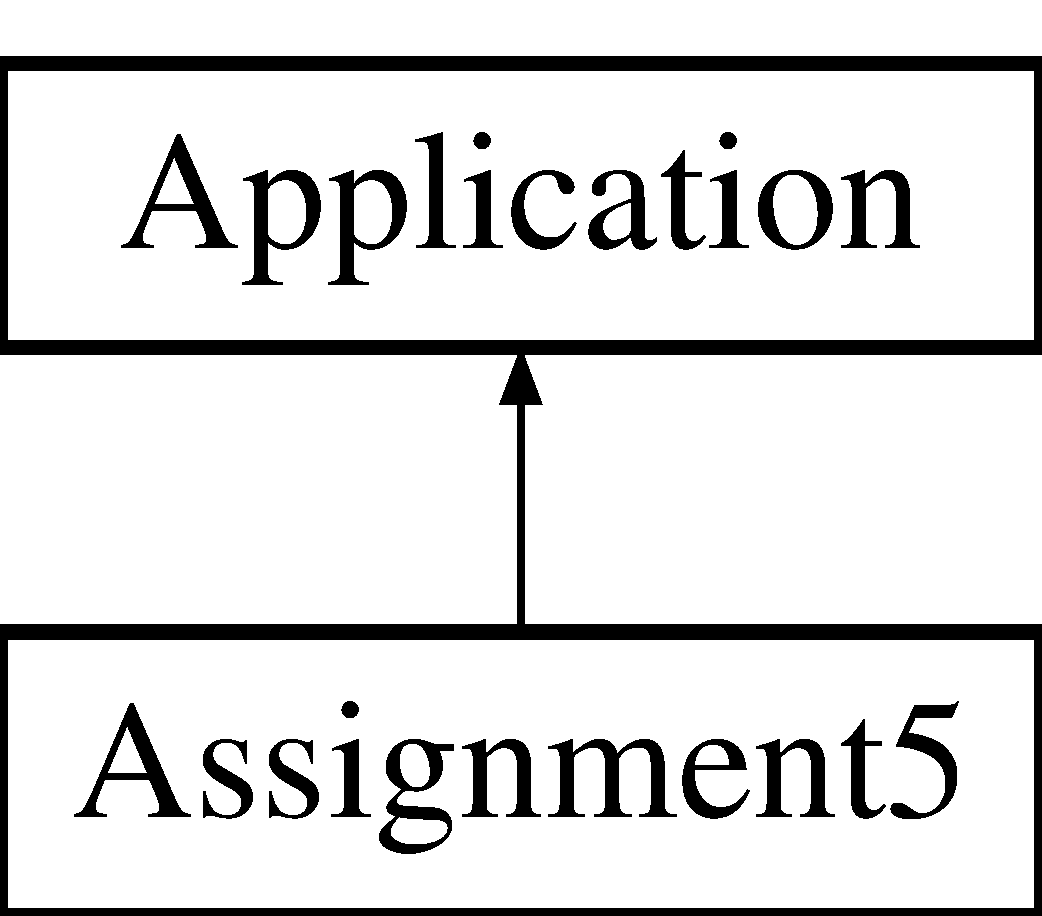
\includegraphics[height=2.000000cm]{class_assignment5}
\end{center}
\end{figure}
\subsection*{Public Member Functions}
\begin{DoxyCompactItemize}
\item
\hyperlink{class_assignment5_aee966f6188c377fd831e6edb97d1ee08}{Assignment5} (std\+::shared\+\_\+ptr$<$ class \hyperlink{class_scene}{Scene} $>$ input\+Scene, std\+::shared\+\_\+ptr$<$ class \hyperlink{class_camera}{Camera} $>$ input\+Camera)
\item
virtual glm\+::vec2 \hyperlink{class_assignment5_ac199b6149ffa3dbedc7e0d49bb24c628}{Get\+Window\+Size} () const
\begin{DoxyCompactList}\small\item\em Specifies the initial window size. \end{DoxyCompactList}\item
virtual void \hyperlink{class_assignment5_aab8f8440144665db9aafd7ca1cf55cff}{Handle\+Input} (S\+D\+L\+\_\+\+Keysym key, Uint32 state, Uint8 repeat, double timestamp, double delta\+Time)
\begin{DoxyCompactList}\small\item\em Processes an S\+DL keyboard event which has type \href{https://wiki.libsdl.org/SDL_KeyboardEvent}{\tt S\+D\+L\+\_\+\+Keyboard\+Event}. \end{DoxyCompactList}\item
virtual void \hyperlink{class_assignment5_a34cdf7bc962c3a0e3959c77a24c54d79}{Tick} (double delta\+Time)
\begin{DoxyCompactList}\small\item\em Called every frame to advance program logic. \end{DoxyCompactList}\end{DoxyCompactItemize}
\subsection*{Static Public Member Functions}
\begin{DoxyCompactItemize}
\item
static std\+::unique\+\_\+ptr$<$ \hyperlink{class_application}{Application} $>$ \hyperlink{class_assignment5_a1b720b74cc23d4f64ced6d2867f2ac63}{Create\+Application} (std\+::shared\+\_\+ptr$<$ class \hyperlink{class_scene}{Scene} $>$ \hyperlink{class_application_a88c6615107a5094bb93fa5f153f79554}{scene}, std\+::shared\+\_\+ptr$<$ class \hyperlink{class_camera}{Camera} $>$ \hyperlink{class_application_a0e8589fcb13c520ba472473abe5a518d}{camera})
\item
static std\+::shared\+\_\+ptr$<$ class \hyperlink{class_camera}{Camera} $>$ \hyperlink{class_assignment5_af80167ddbf48815460a463fc704eb2ce}{Create\+Camera} ()
\end{DoxyCompactItemize}
\subsection*{Protected Member Functions}
\begin{DoxyCompactItemize}
\item
virtual void \hyperlink{class_assignment5_a0e7325af72d41b95f9a19ebe1440e756}{Handle\+Window\+Resize} (float x, float y)
\begin{DoxyCompactList}\small\item\em Called by \hyperlink{class_application_a74d92db64e051efa56d0357989dcb755}{Handle\+Window\+Event()} when the window is resized. \end{DoxyCompactList}\end{DoxyCompactItemize}
\subsection*{Private Member Functions}
\begin{DoxyCompactItemize}
\item
virtual void \hyperlink{class_assignment5_a43328e09e6241ae6c62a9b7be7659b3b}{Setup\+Scene} ()
\begin{DoxyCompactList}\small\item\em Called by \hyperlink{class_application_a17cf1ea4552d26a1c20f7d98d793d41d}{Initialize()} to populate the scene. \end{DoxyCompactList}\item
virtual void \hyperlink{class_assignment5_ad2a3f3271ee7aa69dec95ccf7a95f224}{Setup\+Example1} ()
\item
virtual void \hyperlink{class_assignment5_ad8bde7598ac25e86667a2b0cb45ef399}{Setup\+Example2} ()
\item
virtual void \hyperlink{class_assignment5_a0c49123e133adfb36c769c943eae42fa}{Setup\+Camera} ()
\begin{DoxyCompactList}\small\item\em Called by \hyperlink{class_application_a17cf1ea4552d26a1c20f7d98d793d41d}{Initialize()} to setup the camera. \end{DoxyCompactList}\end{DoxyCompactItemize}
\subsection*{Additional Inherited Members}


\subsection{Constructor \& Destructor Documentation}
\hypertarget{class_assignment5_aee966f6188c377fd831e6edb97d1ee08}{}\label{class_assignment5_aee966f6188c377fd831e6edb97d1ee08}
\index{Assignment5@{Assignment5}!Assignment5@{Assignment5}}
\index{Assignment5@{Assignment5}!Assignment5@{Assignment5}}
\subsubsection{\texorpdfstring{Assignment5()}{Assignment5()}}
{\footnotesize\ttfamily Assignment5\+::\+Assignment5 (\begin{DoxyParamCaption}\item[{std\+::shared\+\_\+ptr$<$ class \hyperlink{class_scene}{Scene} $>$}]{input\+Scene,  }\item[{std\+::shared\+\_\+ptr$<$ class \hyperlink{class_camera}{Camera} $>$}]{input\+Camera }\end{DoxyParamCaption})}



\subsection{Member Function Documentation}
\hypertarget{class_assignment5_a1b720b74cc23d4f64ced6d2867f2ac63}{}\label{class_assignment5_a1b720b74cc23d4f64ced6d2867f2ac63}
\index{Assignment5@{Assignment5}!Create\+Application@{Create\+Application}}
\index{Create\+Application@{Create\+Application}!Assignment5@{Assignment5}}
\subsubsection{\texorpdfstring{Create\+Application()}{CreateApplication()}}
{\footnotesize\ttfamily std\+::unique\+\_\+ptr$<$ \hyperlink{class_application}{Application} $>$ Assignment5\+::\+Create\+Application (\begin{DoxyParamCaption}\item[{std\+::shared\+\_\+ptr$<$ class \hyperlink{class_scene}{Scene} $>$}]{scene,  }\item[{std\+::shared\+\_\+ptr$<$ class \hyperlink{class_camera}{Camera} $>$}]{camera }\end{DoxyParamCaption})\hspace{0.3cm}{\ttfamily [static]}}

\hypertarget{class_assignment5_af80167ddbf48815460a463fc704eb2ce}{}\label{class_assignment5_af80167ddbf48815460a463fc704eb2ce}
\index{Assignment5@{Assignment5}!Create\+Camera@{Create\+Camera}}
\index{Create\+Camera@{Create\+Camera}!Assignment5@{Assignment5}}
\subsubsection{\texorpdfstring{Create\+Camera()}{CreateCamera()}}
{\footnotesize\ttfamily std\+::shared\+\_\+ptr$<$ class \hyperlink{class_camera}{Camera} $>$ Assignment5\+::\+Create\+Camera (\begin{DoxyParamCaption}{ }\end{DoxyParamCaption})\hspace{0.3cm}{\ttfamily [static]}}

\hypertarget{class_assignment5_ac199b6149ffa3dbedc7e0d49bb24c628}{}\label{class_assignment5_ac199b6149ffa3dbedc7e0d49bb24c628}
\index{Assignment5@{Assignment5}!Get\+Window\+Size@{Get\+Window\+Size}}
\index{Get\+Window\+Size@{Get\+Window\+Size}!Assignment5@{Assignment5}}
\subsubsection{\texorpdfstring{Get\+Window\+Size()}{GetWindowSize()}}
{\footnotesize\ttfamily glm\+::vec2 Assignment5\+::\+Get\+Window\+Size (\begin{DoxyParamCaption}{ }\end{DoxyParamCaption}) const\hspace{0.3cm}{\ttfamily [virtual]}}



Specifies the initial window size.

\begin{DoxyReturn}{Returns}
The desired window size.
\end{DoxyReturn}


Reimplemented from \hyperlink{class_application_ab190ae0e987fe95682714dd4b2495e82}{Application}.

\hypertarget{class_assignment5_aab8f8440144665db9aafd7ca1cf55cff}{}\label{class_assignment5_aab8f8440144665db9aafd7ca1cf55cff}
\index{Assignment5@{Assignment5}!Handle\+Input@{Handle\+Input}}
\index{Handle\+Input@{Handle\+Input}!Assignment5@{Assignment5}}
\subsubsection{\texorpdfstring{Handle\+Input()}{HandleInput()}}
{\footnotesize\ttfamily void Assignment5\+::\+Handle\+Input (\begin{DoxyParamCaption}\item[{S\+D\+L\+\_\+\+Keysym}]{key,  }\item[{Uint32}]{state,  }\item[{Uint8}]{repeat,  }\item[{double}]{timestamp,  }\item[{double}]{delta\+Time }\end{DoxyParamCaption})\hspace{0.3cm}{\ttfamily [virtual]}}



Processes an S\+DL keyboard event which has type \href{https://wiki.libsdl.org/SDL_KeyboardEvent}{\tt S\+D\+L\+\_\+\+Keyboard\+Event}.


\begin{DoxyParams}{Parameters}
{\em key} & See the S\+DL documentation for more details about \href{https://wiki.libsdl.org/SDL_Keysym}{\tt S\+D\+L\+\_\+\+Keysym}. \\
\hline
{\em state} & This is the type field in the \href{https://wiki.libsdl.org/SDL_Event}{\tt S\+D\+L\+\_\+\+Event}datastructure. \\
\hline
{\em repeat} & This value is non-\/zero is the key is being repeated. \\
\hline
{\em timestamp} & Timestamp is the number of seconds since the program was first started. \\
\hline
{\em delta\+Time} & The amount of time (in seconds) since the last tick.\\
\hline
\end{DoxyParams}
Takes in a keyboard event and process it. This does nothing by default. \textquotesingle{}delta\+Time\textquotesingle{} is included to allow you to move something and have the movement look smooth. For example, if you have an object that you want to move forward whenever \textquotesingle{}W\textquotesingle{} is pressed. You know that the object travels at 10 meters per second when \textquotesingle{}W\textquotesingle{} is pressed and 0 meters per second when it is not. How far should you move the object? You would want to move it forward by $10 \cdot deltaTime $ units.

Reimplemented from \hyperlink{class_application_ae6074c3f102de1cb2fe4c81b545679db}{Application}.

\hypertarget{class_assignment5_a0e7325af72d41b95f9a19ebe1440e756}{}\label{class_assignment5_a0e7325af72d41b95f9a19ebe1440e756}
\index{Assignment5@{Assignment5}!Handle\+Window\+Resize@{Handle\+Window\+Resize}}
\index{Handle\+Window\+Resize@{Handle\+Window\+Resize}!Assignment5@{Assignment5}}
\subsubsection{\texorpdfstring{Handle\+Window\+Resize()}{HandleWindowResize()}}
{\footnotesize\ttfamily void Assignment5\+::\+Handle\+Window\+Resize (\begin{DoxyParamCaption}\item[{float}]{x,  }\item[{float}]{y }\end{DoxyParamCaption})\hspace{0.3cm}{\ttfamily [protected]}, {\ttfamily [virtual]}}



Called by \hyperlink{class_application_a74d92db64e051efa56d0357989dcb755}{Handle\+Window\+Event()} when the window is resized.


\begin{DoxyParams}{Parameters}
{\em x} & The width of the window. \\
\hline
{\em y} & The height of the window.\\
\hline
\end{DoxyParams}
By default calls, \href{https://www.opengl.org/sdk/docs/man/html/glViewport.xhtml}{\tt gl\+Viewport} to resize the viewport as necessary. If any part of your application depends on the window resize, you will want to take care of it in this function! (Hint for the O\+P\+T\+I\+O\+N\+AL deferred rendering task in assignment 2\+: your \textquotesingle{}G-\/\+Buffers\textquotesingle{} should be resized).

Reimplemented from \hyperlink{class_application_abdba284a0f075ee1d4a2108c3a5236a2}{Application}.

\hypertarget{class_assignment5_a0c49123e133adfb36c769c943eae42fa}{}\label{class_assignment5_a0c49123e133adfb36c769c943eae42fa}
\index{Assignment5@{Assignment5}!Setup\+Camera@{Setup\+Camera}}
\index{Setup\+Camera@{Setup\+Camera}!Assignment5@{Assignment5}}
\subsubsection{\texorpdfstring{Setup\+Camera()}{SetupCamera()}}
{\footnotesize\ttfamily void Assignment5\+::\+Setup\+Camera (\begin{DoxyParamCaption}{ }\end{DoxyParamCaption})\hspace{0.3cm}{\ttfamily [private]}, {\ttfamily [virtual]}}



Called by \hyperlink{class_application_a17cf1ea4552d26a1c20f7d98d793d41d}{Initialize()} to setup the camera.

Note by the time this function is called, the \hyperlink{class_application}{Application} sub-\/class is fully constructed and \hyperlink{class_camera}{Camera} object is already created.

Reimplemented from \hyperlink{class_application_a2eb61ca027f223a5c5ad1bf982481193}{Application}.

\hypertarget{class_assignment5_ad2a3f3271ee7aa69dec95ccf7a95f224}{}\label{class_assignment5_ad2a3f3271ee7aa69dec95ccf7a95f224}
\index{Assignment5@{Assignment5}!Setup\+Example1@{Setup\+Example1}}
\index{Setup\+Example1@{Setup\+Example1}!Assignment5@{Assignment5}}
\subsubsection{\texorpdfstring{Setup\+Example1()}{SetupExample1()}}
{\footnotesize\ttfamily void Assignment5\+::\+Setup\+Example1 (\begin{DoxyParamCaption}{ }\end{DoxyParamCaption})\hspace{0.3cm}{\ttfamily [private]}, {\ttfamily [virtual]}}

\hypertarget{class_assignment5_ad8bde7598ac25e86667a2b0cb45ef399}{}\label{class_assignment5_ad8bde7598ac25e86667a2b0cb45ef399}
\index{Assignment5@{Assignment5}!Setup\+Example2@{Setup\+Example2}}
\index{Setup\+Example2@{Setup\+Example2}!Assignment5@{Assignment5}}
\subsubsection{\texorpdfstring{Setup\+Example2()}{SetupExample2()}}
{\footnotesize\ttfamily void Assignment5\+::\+Setup\+Example2 (\begin{DoxyParamCaption}{ }\end{DoxyParamCaption})\hspace{0.3cm}{\ttfamily [private]}, {\ttfamily [virtual]}}

\hypertarget{class_assignment5_a43328e09e6241ae6c62a9b7be7659b3b}{}\label{class_assignment5_a43328e09e6241ae6c62a9b7be7659b3b}
\index{Assignment5@{Assignment5}!Setup\+Scene@{Setup\+Scene}}
\index{Setup\+Scene@{Setup\+Scene}!Assignment5@{Assignment5}}
\subsubsection{\texorpdfstring{Setup\+Scene()}{SetupScene()}}
{\footnotesize\ttfamily void Assignment5\+::\+Setup\+Scene (\begin{DoxyParamCaption}{ }\end{DoxyParamCaption})\hspace{0.3cm}{\ttfamily [private]}, {\ttfamily [virtual]}}



Called by \hyperlink{class_application_a17cf1ea4552d26a1c20f7d98d793d41d}{Initialize()} to populate the scene.

Note by the time this function is called, the \hyperlink{class_application}{Application} sub-\/class is fully constructed and \hyperlink{class_scene}{Scene} object is already created.

Reimplemented from \hyperlink{class_application_aa8e8017ef8dd86293c96d0645e66d440}{Application}.

\hypertarget{class_assignment5_a34cdf7bc962c3a0e3959c77a24c54d79}{}\label{class_assignment5_a34cdf7bc962c3a0e3959c77a24c54d79}
\index{Assignment5@{Assignment5}!Tick@{Tick}}
\index{Tick@{Tick}!Assignment5@{Assignment5}}
\subsubsection{\texorpdfstring{Tick()}{Tick()}}
{\footnotesize\ttfamily void Assignment5\+::\+Tick (\begin{DoxyParamCaption}\item[{double}]{delta\+Time }\end{DoxyParamCaption})\hspace{0.3cm}{\ttfamily [virtual]}}



Called every frame to advance program logic.


\begin{DoxyParams}{Parameters}
{\em delta\+Time} & The amount of time (in seconds) since the last tick.\\
\hline
\end{DoxyParams}
If you need something in the \hyperlink{class_scene}{Scene} to change over time, this is where you should implement that logic. It is recommended that you make use of the delta\+Time variable to make things change smoothly!

Reimplemented from \hyperlink{class_application_a0800afd5651153d31fa775a8048d14dd}{Application}.



The documentation for this class was generated from the following files\+:\begin{DoxyCompactItemize}
\item
/data/MO814A-MC937A/MO814A-MC937Aopengl-\/instructor/source/assignment5/\hyperlink{_assignment5_8h}{Assignment5.\+h}\item
/data/MO814A-MC937A/MO814A-MC937Aopengl-\/instructor/source/assignment5/\hyperlink{_assignment5_8cpp}{Assignment5.\+cpp}\end{DoxyCompactItemize}

\hypertarget{class_blinn_phong_shader}{}\section{Blinn\+Phong\+Shader Class Reference}
\label{class_blinn_phong_shader}\index{Blinn\+Phong\+Shader@{Blinn\+Phong\+Shader}}


The C\+PU Interface to the Blinn\+Phong shader (either or\+: vert or frag version or the textured version).




{\ttfamily \#include $<$Blinn\+Phong\+Shader.\+h$>$}

Inheritance diagram for Blinn\+Phong\+Shader\+:\begin{figure}[H]
\begin{center}
\leavevmode
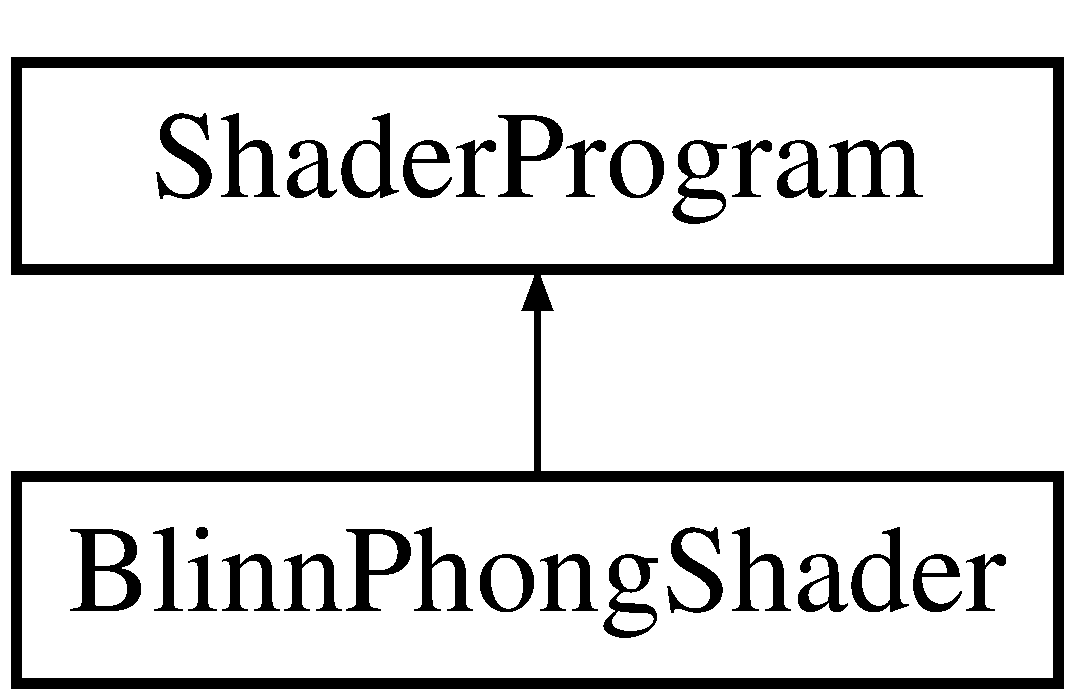
\includegraphics[height=2.000000cm]{class_blinn_phong_shader}
\end{center}
\end{figure}
\subsection*{Classes}
\begin{DoxyCompactItemize}
\item
struct \hyperlink{struct_blinn_phong_shader_1_1_texture_slots}{Texture\+Slots}
\begin{DoxyCompactList}\small\item\em Corresponds to the texture unit that we want to bind the texture to. \end{DoxyCompactList}\end{DoxyCompactItemize}
\subsection*{Public Member Functions}
\begin{DoxyCompactItemize}
\item
\hyperlink{class_blinn_phong_shader_a2a13c983ffcc8d95ffe1a431bb2b1fb6}{Blinn\+Phong\+Shader} (const std\+::unordered\+\_\+map$<$ G\+Lenum, std\+::string $>$ \&input\+Shaders, G\+Lenum lighting\+Stage)
\begin{DoxyCompactList}\small\item\em Construcs the Blinn-\/\+Phong shader object. \end{DoxyCompactList}\item
virtual \hyperlink{class_blinn_phong_shader_a5d7a46de957e0676ed4ceb00f7399a39}{$\sim$\+Blinn\+Phong\+Shader} ()
\begin{DoxyCompactList}\small\item\em Deconstructor. \end{DoxyCompactList}\item
virtual void \hyperlink{class_blinn_phong_shader_a812ffd751068ae3bfc131ddb27712941}{Setup\+Shader\+Lighting} (const class \hyperlink{class_light}{Light} $\ast$light) const
\begin{DoxyCompactList}\small\item\em This function will pass to the G\+L\+SL shader the variables needed by the shader to accurately shade the model using the given light.; \end{DoxyCompactList}\item
virtual void \hyperlink{class_blinn_phong_shader_a444db9ffe3d55dbbb55ced8cf4abb705}{Setup\+Shader\+Materials} () const
\begin{DoxyCompactList}\small\item\em Sets up the shader material (what this material is depends on the shader). \end{DoxyCompactList}\item
virtual void \hyperlink{class_blinn_phong_shader_ab4d435ed4f4815a71590b514550dc2b7}{Setup\+Shader\+Camera} (const class \hyperlink{class_camera}{Camera} $\ast$camera) const
\begin{DoxyCompactList}\small\item\em Passes camera parameters to the shader if necessary. \end{DoxyCompactList}\item
virtual void \hyperlink{class_blinn_phong_shader_a610957f435f1ef817e7d2c4350e55181}{Set\+Diffuse} (glm\+::vec4 in\+Diffuse)
\begin{DoxyCompactList}\small\item\em Sets the diffuse color of the material. \end{DoxyCompactList}\item
virtual void \hyperlink{class_blinn_phong_shader_a6567423da36050cc1567919707e8be72}{Set\+Specular} (glm\+::vec4 in\+Specular, float in\+Shininess)
\begin{DoxyCompactList}\small\item\em Sets the specular color of the material. \end{DoxyCompactList}\item
virtual void \hyperlink{class_blinn_phong_shader_a0f8c1c478525dd662922597ea7d9c4ac}{Set\+Ambient} (glm\+::vec4 in\+Ambient)
\begin{DoxyCompactList}\small\item\em Sets the ambient color of the material. \end{DoxyCompactList}\item
virtual void \hyperlink{class_blinn_phong_shader_aa9c8908b300ce1451887945fb961d3b2}{Set\+Texture} (\hyperlink{struct_blinn_phong_shader_1_1_texture_slots_a98940b49ba855ee47d61a6243c05c34d}{Texture\+Slots\+::\+Type} slot, std\+::shared\+\_\+ptr$<$ class \hyperlink{class_texture}{Texture} $>$ input\+Texture)
\begin{DoxyCompactList}\small\item\em Stores the texture internally. Does not copy to Open\+GL. \end{DoxyCompactList}\item
virtual void \hyperlink{class_blinn_phong_shader_acbef23fe1f5ea72a10dc6ded656dacf0}{Set\+Max\+Displacement} (float input)
\item
virtual void \hyperlink{class_blinn_phong_shader_a5a2a720a403f3d005b07a96fee35b95b}{Load\+Material\+From\+Assimp} (std\+::shared\+\_\+ptr$<$ struct ai\+Material $>$ assimp\+Material)
\end{DoxyCompactItemize}
\subsection*{Protected Member Functions}
\begin{DoxyCompactItemize}
\item
virtual void \hyperlink{class_blinn_phong_shader_aa247270120b46431b436220ea6e777be}{Update\+Material\+Block} () const
\item
virtual void \hyperlink{class_blinn_phong_shader_a389b3b5fea85eb6deedfc028c4140632}{Update\+Attenuation\+Uniforms} (const class \hyperlink{class_light}{Light} $\ast$light) const
\end{DoxyCompactItemize}
\subsection*{Protected Attributes}
\begin{DoxyCompactItemize}
\item
glm\+::vec4 \hyperlink{class_blinn_phong_shader_ae74d0446ec1a871ca57caf002f52e20c}{diffuse}
\item
glm\+::vec4 \hyperlink{class_blinn_phong_shader_a7adce7364e850b9f232e058956f809b8}{specular}
\item
float \hyperlink{class_blinn_phong_shader_ad499c2389d7007ecb4c03d5270314933}{shininess}
\item
glm\+::vec4 \hyperlink{class_blinn_phong_shader_af612b03df22b2bc9e37dcd85124ee9d2}{ambient}
\item
G\+Luint \hyperlink{class_blinn_phong_shader_a4dcd123c2284945734df697501dca5ea}{material\+Block\+Location}
\item
G\+Lint \hyperlink{class_blinn_phong_shader_af38b3d042773f6568f0f6c227de85990}{material\+Block\+Size}
\item
std\+::array$<$ G\+Luint, 4 $>$ \hyperlink{class_blinn_phong_shader_a2b14622a5d0f8ca32c05cc387700692a}{material\+Indices}
\item
std\+::array$<$ G\+Lint, 4 $>$ \hyperlink{class_blinn_phong_shader_a145f22608d6e32a4ec5df39388ad0530}{material\+Offsets}
\item
G\+Luint \hyperlink{class_blinn_phong_shader_a85dbf4a8376a98570a06d9df17938cf4}{material\+Buffer}
\item
std\+::vector$<$ G\+Lubyte $>$ \hyperlink{class_blinn_phong_shader_a7c9644732d35c788d1c94f44b7783d83}{material\+Storage}
\end{DoxyCompactItemize}
\subsection*{Static Protected Attributes}
\begin{DoxyCompactItemize}
\item
static std\+::array$<$ const char $\ast$, 4 $>$ \hyperlink{class_blinn_phong_shader_a6bb55aa4f7aa8b54b127b93386e36dc2}{M\+A\+T\+E\+R\+I\+A\+L\+\_\+\+P\+R\+O\+P\+E\+R\+T\+Y\+\_\+\+N\+A\+M\+ES}
\item
static const int \hyperlink{class_blinn_phong_shader_a44b4e326871466fe9f2346eb1ac40253}{M\+A\+T\+E\+R\+I\+A\+L\+\_\+\+B\+I\+N\+D\+I\+N\+G\+\_\+\+P\+O\+I\+NT} = 0
\end{DoxyCompactItemize}
\subsection*{Private Attributes}
\begin{DoxyCompactItemize}
\item
std\+::shared\+\_\+ptr$<$ class \hyperlink{class_texture}{Texture} $>$ \hyperlink{class_blinn_phong_shader_a2335cf5c2d95098a94f9f2e888b329f3}{default\+Texture}
\item
std\+::unordered\+\_\+map$<$ \hyperlink{struct_blinn_phong_shader_1_1_texture_slots_a98940b49ba855ee47d61a6243c05c34d}{Texture\+Slots\+::\+Type}, std\+::shared\+\_\+ptr$<$ class \hyperlink{class_texture}{Texture} $>$, std\+::hash$<$ int $>$ $>$ \hyperlink{class_blinn_phong_shader_a7467b1de2650fd04ea63ed5f8aeedc59}{texture\+Slot\+Mapping}
\item
G\+Lenum \hyperlink{class_blinn_phong_shader_a942775771a09fd5553409bdb44ec32ac}{lighting\+Shader\+Stage}
\item
float \hyperlink{class_blinn_phong_shader_a9e5e58c4901d48b315e94d15fd504a8c}{max\+Displacement}
\end{DoxyCompactItemize}
\subsection*{Additional Inherited Members}


\subsection{Detailed Description}
The C\+PU Interface to the Blinn\+Phong shader (either or\+: vert or frag version or the textured version).

Note that this shader class can also probably be used for any minor variations on the Blinn-\/\+Phong shader.

\subsection{Constructor \& Destructor Documentation}
\hypertarget{class_blinn_phong_shader_a2a13c983ffcc8d95ffe1a431bb2b1fb6}{}\label{class_blinn_phong_shader_a2a13c983ffcc8d95ffe1a431bb2b1fb6}
\index{Blinn\+Phong\+Shader@{Blinn\+Phong\+Shader}!Blinn\+Phong\+Shader@{Blinn\+Phong\+Shader}}
\index{Blinn\+Phong\+Shader@{Blinn\+Phong\+Shader}!Blinn\+Phong\+Shader@{Blinn\+Phong\+Shader}}
\subsubsection{\texorpdfstring{Blinn\+Phong\+Shader()}{BlinnPhongShader()}}
{\footnotesize\ttfamily Blinn\+Phong\+Shader\+::\+Blinn\+Phong\+Shader (\begin{DoxyParamCaption}\item[{const std\+::unordered\+\_\+map$<$ G\+Lenum, std\+::string $>$ \&}]{input\+Shaders,  }\item[{G\+Lenum}]{lighting\+Stage }\end{DoxyParamCaption})}



Construcs the Blinn-\/\+Phong shader object.


\begin{DoxyParams}{Parameters}
{\em input\+Shaders} & Look at \hyperlink{class_shader_program_aba2db5734b2f70cc34078126ad279588}{Shader\+Program\+::\+Shader\+Program()} for details. \\
\hline
{\em lighting\+Stage} & If subroutines are not disabled, this is the shader object (vertex or fragment) that contains the subroutine uniform variable. \\
\hline
\end{DoxyParams}
\hypertarget{class_blinn_phong_shader_a5d7a46de957e0676ed4ceb00f7399a39}{}\label{class_blinn_phong_shader_a5d7a46de957e0676ed4ceb00f7399a39}
\index{Blinn\+Phong\+Shader@{Blinn\+Phong\+Shader}!````~Blinn\+Phong\+Shader@{$\sim$\+Blinn\+Phong\+Shader}}
\index{````~Blinn\+Phong\+Shader@{$\sim$\+Blinn\+Phong\+Shader}!Blinn\+Phong\+Shader@{Blinn\+Phong\+Shader}}
\subsubsection{\texorpdfstring{$\sim$\+Blinn\+Phong\+Shader()}{~BlinnPhongShader()}}
{\footnotesize\ttfamily Blinn\+Phong\+Shader\+::$\sim$\+Blinn\+Phong\+Shader (\begin{DoxyParamCaption}{ }\end{DoxyParamCaption})\hspace{0.3cm}{\ttfamily [virtual]}}



Deconstructor.



\subsection{Member Function Documentation}
\hypertarget{class_blinn_phong_shader_a5a2a720a403f3d005b07a96fee35b95b}{}\label{class_blinn_phong_shader_a5a2a720a403f3d005b07a96fee35b95b}
\index{Blinn\+Phong\+Shader@{Blinn\+Phong\+Shader}!Load\+Material\+From\+Assimp@{Load\+Material\+From\+Assimp}}
\index{Load\+Material\+From\+Assimp@{Load\+Material\+From\+Assimp}!Blinn\+Phong\+Shader@{Blinn\+Phong\+Shader}}
\subsubsection{\texorpdfstring{Load\+Material\+From\+Assimp()}{LoadMaterialFromAssimp()}}
{\footnotesize\ttfamily void Blinn\+Phong\+Shader\+::\+Load\+Material\+From\+Assimp (\begin{DoxyParamCaption}\item[{std\+::shared\+\_\+ptr$<$ struct ai\+Material $>$}]{assimp\+Material }\end{DoxyParamCaption})\hspace{0.3cm}{\ttfamily [virtual]}}



Reimplemented from \hyperlink{class_shader_program_a51ac6fbf3a3d88643eef303a4c3a1fa8}{Shader\+Program}.

\hypertarget{class_blinn_phong_shader_a0f8c1c478525dd662922597ea7d9c4ac}{}\label{class_blinn_phong_shader_a0f8c1c478525dd662922597ea7d9c4ac}
\index{Blinn\+Phong\+Shader@{Blinn\+Phong\+Shader}!Set\+Ambient@{Set\+Ambient}}
\index{Set\+Ambient@{Set\+Ambient}!Blinn\+Phong\+Shader@{Blinn\+Phong\+Shader}}
\subsubsection{\texorpdfstring{Set\+Ambient()}{SetAmbient()}}
{\footnotesize\ttfamily void Blinn\+Phong\+Shader\+::\+Set\+Ambient (\begin{DoxyParamCaption}\item[{glm\+::vec4}]{in\+Ambient }\end{DoxyParamCaption})\hspace{0.3cm}{\ttfamily [virtual]}}



Sets the ambient color of the material.


\begin{DoxyParams}{Parameters}
{\em in\+Ambient} & The desired ambient color.\\
\hline
\end{DoxyParams}
Immediately calls \hyperlink{class_blinn_phong_shader_aa247270120b46431b436220ea6e777be}{Update\+Material\+Block()} to store the new data into the Open\+GL buffer. \hypertarget{class_blinn_phong_shader_a610957f435f1ef817e7d2c4350e55181}{}\label{class_blinn_phong_shader_a610957f435f1ef817e7d2c4350e55181}
\index{Blinn\+Phong\+Shader@{Blinn\+Phong\+Shader}!Set\+Diffuse@{Set\+Diffuse}}
\index{Set\+Diffuse@{Set\+Diffuse}!Blinn\+Phong\+Shader@{Blinn\+Phong\+Shader}}
\subsubsection{\texorpdfstring{Set\+Diffuse()}{SetDiffuse()}}
{\footnotesize\ttfamily void Blinn\+Phong\+Shader\+::\+Set\+Diffuse (\begin{DoxyParamCaption}\item[{glm\+::vec4}]{in\+Diffuse }\end{DoxyParamCaption})\hspace{0.3cm}{\ttfamily [virtual]}}



Sets the diffuse color of the material.


\begin{DoxyParams}{Parameters}
{\em in\+Diffuse} & The desired diffuse color.\\
\hline
\end{DoxyParams}
Immediately calls \hyperlink{class_blinn_phong_shader_aa247270120b46431b436220ea6e777be}{Update\+Material\+Block()} to store the new data into the Open\+GL buffer. \hypertarget{class_blinn_phong_shader_acbef23fe1f5ea72a10dc6ded656dacf0}{}\label{class_blinn_phong_shader_acbef23fe1f5ea72a10dc6ded656dacf0}
\index{Blinn\+Phong\+Shader@{Blinn\+Phong\+Shader}!Set\+Max\+Displacement@{Set\+Max\+Displacement}}
\index{Set\+Max\+Displacement@{Set\+Max\+Displacement}!Blinn\+Phong\+Shader@{Blinn\+Phong\+Shader}}
\subsubsection{\texorpdfstring{Set\+Max\+Displacement()}{SetMaxDisplacement()}}
{\footnotesize\ttfamily void Blinn\+Phong\+Shader\+::\+Set\+Max\+Displacement (\begin{DoxyParamCaption}\item[{float}]{input }\end{DoxyParamCaption})\hspace{0.3cm}{\ttfamily [virtual]}}

\hypertarget{class_blinn_phong_shader_a6567423da36050cc1567919707e8be72}{}\label{class_blinn_phong_shader_a6567423da36050cc1567919707e8be72}
\index{Blinn\+Phong\+Shader@{Blinn\+Phong\+Shader}!Set\+Specular@{Set\+Specular}}
\index{Set\+Specular@{Set\+Specular}!Blinn\+Phong\+Shader@{Blinn\+Phong\+Shader}}
\subsubsection{\texorpdfstring{Set\+Specular()}{SetSpecular()}}
{\footnotesize\ttfamily void Blinn\+Phong\+Shader\+::\+Set\+Specular (\begin{DoxyParamCaption}\item[{glm\+::vec4}]{in\+Specular,  }\item[{float}]{in\+Shininess }\end{DoxyParamCaption})\hspace{0.3cm}{\ttfamily [virtual]}}



Sets the specular color of the material.


\begin{DoxyParams}{Parameters}
{\em in\+Specular} & The desired specular color. \\
\hline
{\em in\+Shininess} & The desired shininess.\\
\hline
\end{DoxyParams}
Immediately calls \hyperlink{class_blinn_phong_shader_aa247270120b46431b436220ea6e777be}{Update\+Material\+Block()} to store the new data into the Open\+GL buffer. For more information about the shininess parameters, refer to the Wikipedia page on the \href{https://en.wikipedia.org/wiki/Phong_reflection_model}{\tt Phong reflection model}. \hypertarget{class_blinn_phong_shader_aa9c8908b300ce1451887945fb961d3b2}{}\label{class_blinn_phong_shader_aa9c8908b300ce1451887945fb961d3b2}
\index{Blinn\+Phong\+Shader@{Blinn\+Phong\+Shader}!Set\+Texture@{Set\+Texture}}
\index{Set\+Texture@{Set\+Texture}!Blinn\+Phong\+Shader@{Blinn\+Phong\+Shader}}
\subsubsection{\texorpdfstring{Set\+Texture()}{SetTexture()}}
{\footnotesize\ttfamily void Blinn\+Phong\+Shader\+::\+Set\+Texture (\begin{DoxyParamCaption}\item[{\hyperlink{struct_blinn_phong_shader_1_1_texture_slots_a98940b49ba855ee47d61a6243c05c34d}{Texture\+Slots\+::\+Type}}]{slot,  }\item[{std\+::shared\+\_\+ptr$<$ class \hyperlink{class_texture}{Texture} $>$}]{input\+Texture }\end{DoxyParamCaption})\hspace{0.3cm}{\ttfamily [virtual]}}



Stores the texture internally. Does not copy to Open\+GL.


\begin{DoxyParams}{Parameters}
{\em slot} & The texture unit that we will be binding the texture to. \\
\hline
{\em input\+Texture} & A pointer to the assignment framework\textquotesingle{}s representation of a texture. \\
\hline
\end{DoxyParams}
\hypertarget{class_blinn_phong_shader_ab4d435ed4f4815a71590b514550dc2b7}{}\label{class_blinn_phong_shader_ab4d435ed4f4815a71590b514550dc2b7}
\index{Blinn\+Phong\+Shader@{Blinn\+Phong\+Shader}!Setup\+Shader\+Camera@{Setup\+Shader\+Camera}}
\index{Setup\+Shader\+Camera@{Setup\+Shader\+Camera}!Blinn\+Phong\+Shader@{Blinn\+Phong\+Shader}}
\subsubsection{\texorpdfstring{Setup\+Shader\+Camera()}{SetupShaderCamera()}}
{\footnotesize\ttfamily void Blinn\+Phong\+Shader\+::\+Setup\+Shader\+Camera (\begin{DoxyParamCaption}\item[{const class \hyperlink{class_camera}{Camera} $\ast$}]{camera }\end{DoxyParamCaption}) const\hspace{0.3cm}{\ttfamily [virtual]}}



Passes camera parameters to the shader if necessary.


\begin{DoxyParams}{Parameters}
{\em camera} & The camera we want to use for shading. This should not be a null pointer.\\
\hline
\end{DoxyParams}
Copies the camera position to the shader.

Reimplemented from \hyperlink{class_shader_program_abefd4e66aae75993f05bd607b6b0ed22}{Shader\+Program}.

\hypertarget{class_blinn_phong_shader_a812ffd751068ae3bfc131ddb27712941}{}\label{class_blinn_phong_shader_a812ffd751068ae3bfc131ddb27712941}
\index{Blinn\+Phong\+Shader@{Blinn\+Phong\+Shader}!Setup\+Shader\+Lighting@{Setup\+Shader\+Lighting}}
\index{Setup\+Shader\+Lighting@{Setup\+Shader\+Lighting}!Blinn\+Phong\+Shader@{Blinn\+Phong\+Shader}}
\subsubsection{\texorpdfstring{Setup\+Shader\+Lighting()}{SetupShaderLighting()}}
{\footnotesize\ttfamily void Blinn\+Phong\+Shader\+::\+Setup\+Shader\+Lighting (\begin{DoxyParamCaption}\item[{const class \hyperlink{class_light}{Light} $\ast$}]{light }\end{DoxyParamCaption}) const\hspace{0.3cm}{\ttfamily [virtual]}}



This function will pass to the G\+L\+SL shader the variables needed by the shader to accurately shade the model using the given light.;


\begin{DoxyParams}{Parameters}
{\em light} & The light we want to use for shading. This should not be a null pointer.;\\
\hline
\end{DoxyParams}
Makes sure the proper lighting function is called (i.\+e. for point light, directional, etc.). Additionally, passes in the light properties to the shader as well as any light attenuation properties.

Reimplemented from \hyperlink{class_shader_program_a02cf3df43c59808160fce158ad655a40}{Shader\+Program}.

\hypertarget{class_blinn_phong_shader_a444db9ffe3d55dbbb55ced8cf4abb705}{}\label{class_blinn_phong_shader_a444db9ffe3d55dbbb55ced8cf4abb705}
\index{Blinn\+Phong\+Shader@{Blinn\+Phong\+Shader}!Setup\+Shader\+Materials@{Setup\+Shader\+Materials}}
\index{Setup\+Shader\+Materials@{Setup\+Shader\+Materials}!Blinn\+Phong\+Shader@{Blinn\+Phong\+Shader}}
\subsubsection{\texorpdfstring{Setup\+Shader\+Materials()}{SetupShaderMaterials()}}
{\footnotesize\ttfamily void Blinn\+Phong\+Shader\+::\+Setup\+Shader\+Materials (\begin{DoxyParamCaption}{ }\end{DoxyParamCaption}) const\hspace{0.3cm}{\ttfamily [virtual]}}



Sets up the shader material (what this material is depends on the shader).

This functions is meant to be a general setup function for the shader. This function has no access to the scene or anything else stored in the application so its primary purpose is to work with objects stored within the shader program object (i.\+e. textures).

Makes sure that the uniform block object is bound and handles binding the diffuse and specular textures if they exist.

Reimplemented from \hyperlink{class_shader_program_a20ea5669f122fa6143e7fa8ee9d92578}{Shader\+Program}.

\hypertarget{class_blinn_phong_shader_a389b3b5fea85eb6deedfc028c4140632}{}\label{class_blinn_phong_shader_a389b3b5fea85eb6deedfc028c4140632}
\index{Blinn\+Phong\+Shader@{Blinn\+Phong\+Shader}!Update\+Attenuation\+Uniforms@{Update\+Attenuation\+Uniforms}}
\index{Update\+Attenuation\+Uniforms@{Update\+Attenuation\+Uniforms}!Blinn\+Phong\+Shader@{Blinn\+Phong\+Shader}}
\subsubsection{\texorpdfstring{Update\+Attenuation\+Uniforms()}{UpdateAttenuationUniforms()}}
{\footnotesize\ttfamily void Blinn\+Phong\+Shader\+::\+Update\+Attenuation\+Uniforms (\begin{DoxyParamCaption}\item[{const class \hyperlink{class_light}{Light} $\ast$}]{light }\end{DoxyParamCaption}) const\hspace{0.3cm}{\ttfamily [protected]}, {\ttfamily [virtual]}}

\hypertarget{class_blinn_phong_shader_aa247270120b46431b436220ea6e777be}{}\label{class_blinn_phong_shader_aa247270120b46431b436220ea6e777be}
\index{Blinn\+Phong\+Shader@{Blinn\+Phong\+Shader}!Update\+Material\+Block@{Update\+Material\+Block}}
\index{Update\+Material\+Block@{Update\+Material\+Block}!Blinn\+Phong\+Shader@{Blinn\+Phong\+Shader}}
\subsubsection{\texorpdfstring{Update\+Material\+Block()}{UpdateMaterialBlock()}}
{\footnotesize\ttfamily void Blinn\+Phong\+Shader\+::\+Update\+Material\+Block (\begin{DoxyParamCaption}{ }\end{DoxyParamCaption}) const\hspace{0.3cm}{\ttfamily [protected]}, {\ttfamily [virtual]}}



\subsection{Member Data Documentation}
\hypertarget{class_blinn_phong_shader_af612b03df22b2bc9e37dcd85124ee9d2}{}\label{class_blinn_phong_shader_af612b03df22b2bc9e37dcd85124ee9d2}
\index{Blinn\+Phong\+Shader@{Blinn\+Phong\+Shader}!ambient@{ambient}}
\index{ambient@{ambient}!Blinn\+Phong\+Shader@{Blinn\+Phong\+Shader}}
\subsubsection{\texorpdfstring{ambient}{ambient}}
{\footnotesize\ttfamily glm\+::vec4 Blinn\+Phong\+Shader\+::ambient\hspace{0.3cm}{\ttfamily [protected]}}

\hypertarget{class_blinn_phong_shader_a2335cf5c2d95098a94f9f2e888b329f3}{}\label{class_blinn_phong_shader_a2335cf5c2d95098a94f9f2e888b329f3}
\index{Blinn\+Phong\+Shader@{Blinn\+Phong\+Shader}!default\+Texture@{default\+Texture}}
\index{default\+Texture@{default\+Texture}!Blinn\+Phong\+Shader@{Blinn\+Phong\+Shader}}
\subsubsection{\texorpdfstring{default\+Texture}{defaultTexture}}
{\footnotesize\ttfamily std\+::shared\+\_\+ptr$<$class \hyperlink{class_texture}{Texture}$>$ Blinn\+Phong\+Shader\+::default\+Texture\hspace{0.3cm}{\ttfamily [private]}}

\hypertarget{class_blinn_phong_shader_ae74d0446ec1a871ca57caf002f52e20c}{}\label{class_blinn_phong_shader_ae74d0446ec1a871ca57caf002f52e20c}
\index{Blinn\+Phong\+Shader@{Blinn\+Phong\+Shader}!diffuse@{diffuse}}
\index{diffuse@{diffuse}!Blinn\+Phong\+Shader@{Blinn\+Phong\+Shader}}
\subsubsection{\texorpdfstring{diffuse}{diffuse}}
{\footnotesize\ttfamily glm\+::vec4 Blinn\+Phong\+Shader\+::diffuse\hspace{0.3cm}{\ttfamily [protected]}}

\hypertarget{class_blinn_phong_shader_a942775771a09fd5553409bdb44ec32ac}{}\label{class_blinn_phong_shader_a942775771a09fd5553409bdb44ec32ac}
\index{Blinn\+Phong\+Shader@{Blinn\+Phong\+Shader}!lighting\+Shader\+Stage@{lighting\+Shader\+Stage}}
\index{lighting\+Shader\+Stage@{lighting\+Shader\+Stage}!Blinn\+Phong\+Shader@{Blinn\+Phong\+Shader}}
\subsubsection{\texorpdfstring{lighting\+Shader\+Stage}{lightingShaderStage}}
{\footnotesize\ttfamily G\+Lenum Blinn\+Phong\+Shader\+::lighting\+Shader\+Stage\hspace{0.3cm}{\ttfamily [private]}}

\hypertarget{class_blinn_phong_shader_a44b4e326871466fe9f2346eb1ac40253}{}\label{class_blinn_phong_shader_a44b4e326871466fe9f2346eb1ac40253}
\index{Blinn\+Phong\+Shader@{Blinn\+Phong\+Shader}!M\+A\+T\+E\+R\+I\+A\+L\+\_\+\+B\+I\+N\+D\+I\+N\+G\+\_\+\+P\+O\+I\+NT@{M\+A\+T\+E\+R\+I\+A\+L\+\_\+\+B\+I\+N\+D\+I\+N\+G\+\_\+\+P\+O\+I\+NT}}
\index{M\+A\+T\+E\+R\+I\+A\+L\+\_\+\+B\+I\+N\+D\+I\+N\+G\+\_\+\+P\+O\+I\+NT@{M\+A\+T\+E\+R\+I\+A\+L\+\_\+\+B\+I\+N\+D\+I\+N\+G\+\_\+\+P\+O\+I\+NT}!Blinn\+Phong\+Shader@{Blinn\+Phong\+Shader}}
\subsubsection{\texorpdfstring{M\+A\+T\+E\+R\+I\+A\+L\+\_\+\+B\+I\+N\+D\+I\+N\+G\+\_\+\+P\+O\+I\+NT}{MATERIAL\_BINDING\_POINT}}
{\footnotesize\ttfamily const int Blinn\+Phong\+Shader\+::\+M\+A\+T\+E\+R\+I\+A\+L\+\_\+\+B\+I\+N\+D\+I\+N\+G\+\_\+\+P\+O\+I\+NT = 0\hspace{0.3cm}{\ttfamily [static]}, {\ttfamily [protected]}}

\hypertarget{class_blinn_phong_shader_a6bb55aa4f7aa8b54b127b93386e36dc2}{}\label{class_blinn_phong_shader_a6bb55aa4f7aa8b54b127b93386e36dc2}
\index{Blinn\+Phong\+Shader@{Blinn\+Phong\+Shader}!M\+A\+T\+E\+R\+I\+A\+L\+\_\+\+P\+R\+O\+P\+E\+R\+T\+Y\+\_\+\+N\+A\+M\+ES@{M\+A\+T\+E\+R\+I\+A\+L\+\_\+\+P\+R\+O\+P\+E\+R\+T\+Y\+\_\+\+N\+A\+M\+ES}}
\index{M\+A\+T\+E\+R\+I\+A\+L\+\_\+\+P\+R\+O\+P\+E\+R\+T\+Y\+\_\+\+N\+A\+M\+ES@{M\+A\+T\+E\+R\+I\+A\+L\+\_\+\+P\+R\+O\+P\+E\+R\+T\+Y\+\_\+\+N\+A\+M\+ES}!Blinn\+Phong\+Shader@{Blinn\+Phong\+Shader}}
\subsubsection{\texorpdfstring{M\+A\+T\+E\+R\+I\+A\+L\+\_\+\+P\+R\+O\+P\+E\+R\+T\+Y\+\_\+\+N\+A\+M\+ES}{MATERIAL\_PROPERTY\_NAMES}}
{\footnotesize\ttfamily std\+::array$<$ const char $\ast$, 4 $>$ Blinn\+Phong\+Shader\+::\+M\+A\+T\+E\+R\+I\+A\+L\+\_\+\+P\+R\+O\+P\+E\+R\+T\+Y\+\_\+\+N\+A\+M\+ES\hspace{0.3cm}{\ttfamily [static]}, {\ttfamily [protected]}}

{\bfseries Initial value\+:}
\begin{DoxyCode}
= \{
    \textcolor{stringliteral}{"InputMaterial.matDiffuse"},
    \textcolor{stringliteral}{"InputMaterial.matSpecular"},
    \textcolor{stringliteral}{"InputMaterial.matShininess"},
    \textcolor{stringliteral}{"InputMaterial.matAmbient"}
\}
\end{DoxyCode}
\hypertarget{class_blinn_phong_shader_a4dcd123c2284945734df697501dca5ea}{}\label{class_blinn_phong_shader_a4dcd123c2284945734df697501dca5ea}
\index{Blinn\+Phong\+Shader@{Blinn\+Phong\+Shader}!material\+Block\+Location@{material\+Block\+Location}}
\index{material\+Block\+Location@{material\+Block\+Location}!Blinn\+Phong\+Shader@{Blinn\+Phong\+Shader}}
\subsubsection{\texorpdfstring{material\+Block\+Location}{materialBlockLocation}}
{\footnotesize\ttfamily G\+Luint Blinn\+Phong\+Shader\+::material\+Block\+Location\hspace{0.3cm}{\ttfamily [protected]}}

\hypertarget{class_blinn_phong_shader_af38b3d042773f6568f0f6c227de85990}{}\label{class_blinn_phong_shader_af38b3d042773f6568f0f6c227de85990}
\index{Blinn\+Phong\+Shader@{Blinn\+Phong\+Shader}!material\+Block\+Size@{material\+Block\+Size}}
\index{material\+Block\+Size@{material\+Block\+Size}!Blinn\+Phong\+Shader@{Blinn\+Phong\+Shader}}
\subsubsection{\texorpdfstring{material\+Block\+Size}{materialBlockSize}}
{\footnotesize\ttfamily G\+Lint Blinn\+Phong\+Shader\+::material\+Block\+Size\hspace{0.3cm}{\ttfamily [protected]}}

\hypertarget{class_blinn_phong_shader_a85dbf4a8376a98570a06d9df17938cf4}{}\label{class_blinn_phong_shader_a85dbf4a8376a98570a06d9df17938cf4}
\index{Blinn\+Phong\+Shader@{Blinn\+Phong\+Shader}!material\+Buffer@{material\+Buffer}}
\index{material\+Buffer@{material\+Buffer}!Blinn\+Phong\+Shader@{Blinn\+Phong\+Shader}}
\subsubsection{\texorpdfstring{material\+Buffer}{materialBuffer}}
{\footnotesize\ttfamily G\+Luint Blinn\+Phong\+Shader\+::material\+Buffer\hspace{0.3cm}{\ttfamily [protected]}}

\hypertarget{class_blinn_phong_shader_a2b14622a5d0f8ca32c05cc387700692a}{}\label{class_blinn_phong_shader_a2b14622a5d0f8ca32c05cc387700692a}
\index{Blinn\+Phong\+Shader@{Blinn\+Phong\+Shader}!material\+Indices@{material\+Indices}}
\index{material\+Indices@{material\+Indices}!Blinn\+Phong\+Shader@{Blinn\+Phong\+Shader}}
\subsubsection{\texorpdfstring{material\+Indices}{materialIndices}}
{\footnotesize\ttfamily std\+::array$<$G\+Luint, 4$>$ Blinn\+Phong\+Shader\+::material\+Indices\hspace{0.3cm}{\ttfamily [protected]}}

\hypertarget{class_blinn_phong_shader_a145f22608d6e32a4ec5df39388ad0530}{}\label{class_blinn_phong_shader_a145f22608d6e32a4ec5df39388ad0530}
\index{Blinn\+Phong\+Shader@{Blinn\+Phong\+Shader}!material\+Offsets@{material\+Offsets}}
\index{material\+Offsets@{material\+Offsets}!Blinn\+Phong\+Shader@{Blinn\+Phong\+Shader}}
\subsubsection{\texorpdfstring{material\+Offsets}{materialOffsets}}
{\footnotesize\ttfamily std\+::array$<$G\+Lint, 4$>$ Blinn\+Phong\+Shader\+::material\+Offsets\hspace{0.3cm}{\ttfamily [protected]}}

\hypertarget{class_blinn_phong_shader_a7c9644732d35c788d1c94f44b7783d83}{}\label{class_blinn_phong_shader_a7c9644732d35c788d1c94f44b7783d83}
\index{Blinn\+Phong\+Shader@{Blinn\+Phong\+Shader}!material\+Storage@{material\+Storage}}
\index{material\+Storage@{material\+Storage}!Blinn\+Phong\+Shader@{Blinn\+Phong\+Shader}}
\subsubsection{\texorpdfstring{material\+Storage}{materialStorage}}
{\footnotesize\ttfamily std\+::vector$<$G\+Lubyte$>$ Blinn\+Phong\+Shader\+::material\+Storage\hspace{0.3cm}{\ttfamily [protected]}}

\hypertarget{class_blinn_phong_shader_a9e5e58c4901d48b315e94d15fd504a8c}{}\label{class_blinn_phong_shader_a9e5e58c4901d48b315e94d15fd504a8c}
\index{Blinn\+Phong\+Shader@{Blinn\+Phong\+Shader}!max\+Displacement@{max\+Displacement}}
\index{max\+Displacement@{max\+Displacement}!Blinn\+Phong\+Shader@{Blinn\+Phong\+Shader}}
\subsubsection{\texorpdfstring{max\+Displacement}{maxDisplacement}}
{\footnotesize\ttfamily float Blinn\+Phong\+Shader\+::max\+Displacement\hspace{0.3cm}{\ttfamily [private]}}

\hypertarget{class_blinn_phong_shader_ad499c2389d7007ecb4c03d5270314933}{}\label{class_blinn_phong_shader_ad499c2389d7007ecb4c03d5270314933}
\index{Blinn\+Phong\+Shader@{Blinn\+Phong\+Shader}!shininess@{shininess}}
\index{shininess@{shininess}!Blinn\+Phong\+Shader@{Blinn\+Phong\+Shader}}
\subsubsection{\texorpdfstring{shininess}{shininess}}
{\footnotesize\ttfamily float Blinn\+Phong\+Shader\+::shininess\hspace{0.3cm}{\ttfamily [protected]}}

\hypertarget{class_blinn_phong_shader_a7adce7364e850b9f232e058956f809b8}{}\label{class_blinn_phong_shader_a7adce7364e850b9f232e058956f809b8}
\index{Blinn\+Phong\+Shader@{Blinn\+Phong\+Shader}!specular@{specular}}
\index{specular@{specular}!Blinn\+Phong\+Shader@{Blinn\+Phong\+Shader}}
\subsubsection{\texorpdfstring{specular}{specular}}
{\footnotesize\ttfamily glm\+::vec4 Blinn\+Phong\+Shader\+::specular\hspace{0.3cm}{\ttfamily [protected]}}

\hypertarget{class_blinn_phong_shader_a7467b1de2650fd04ea63ed5f8aeedc59}{}\label{class_blinn_phong_shader_a7467b1de2650fd04ea63ed5f8aeedc59}
\index{Blinn\+Phong\+Shader@{Blinn\+Phong\+Shader}!texture\+Slot\+Mapping@{texture\+Slot\+Mapping}}
\index{texture\+Slot\+Mapping@{texture\+Slot\+Mapping}!Blinn\+Phong\+Shader@{Blinn\+Phong\+Shader}}
\subsubsection{\texorpdfstring{texture\+Slot\+Mapping}{textureSlotMapping}}
{\footnotesize\ttfamily std\+::unordered\+\_\+map$<$\hyperlink{struct_blinn_phong_shader_1_1_texture_slots_a98940b49ba855ee47d61a6243c05c34d}{Texture\+Slots\+::\+Type}, std\+::shared\+\_\+ptr$<$class \hyperlink{class_texture}{Texture}$>$, std\+::hash$<$int$>$ $>$ Blinn\+Phong\+Shader\+::texture\+Slot\+Mapping\hspace{0.3cm}{\ttfamily [private]}}



The documentation for this class was generated from the following files\+:\begin{DoxyCompactItemize}
\item
/data/MO814A-MC937A/MO814A-MC937Aopengl-\/instructor/source/common/\+Rendering/\+Shaders/\hyperlink{_blinn_phong_shader_8h}{Blinn\+Phong\+Shader.\+h}\item
/data/MO814A-MC937A/MO814A-MC937Aopengl-\/instructor/source/common/\+Rendering/\+Shaders/\hyperlink{_blinn_phong_shader_8cpp}{Blinn\+Phong\+Shader.\+cpp}\end{DoxyCompactItemize}

\hypertarget{class_camera}{}\section{Camera Class Reference}
\label{class_camera}\index{Camera@{Camera}}


The camera interface that also serves as a \char`\"{}null\char`\"{} camera.




{\ttfamily \#include $<$Camera.\+h$>$}

Inheritance diagram for Camera\+:\begin{figure}[H]
\begin{center}
\leavevmode
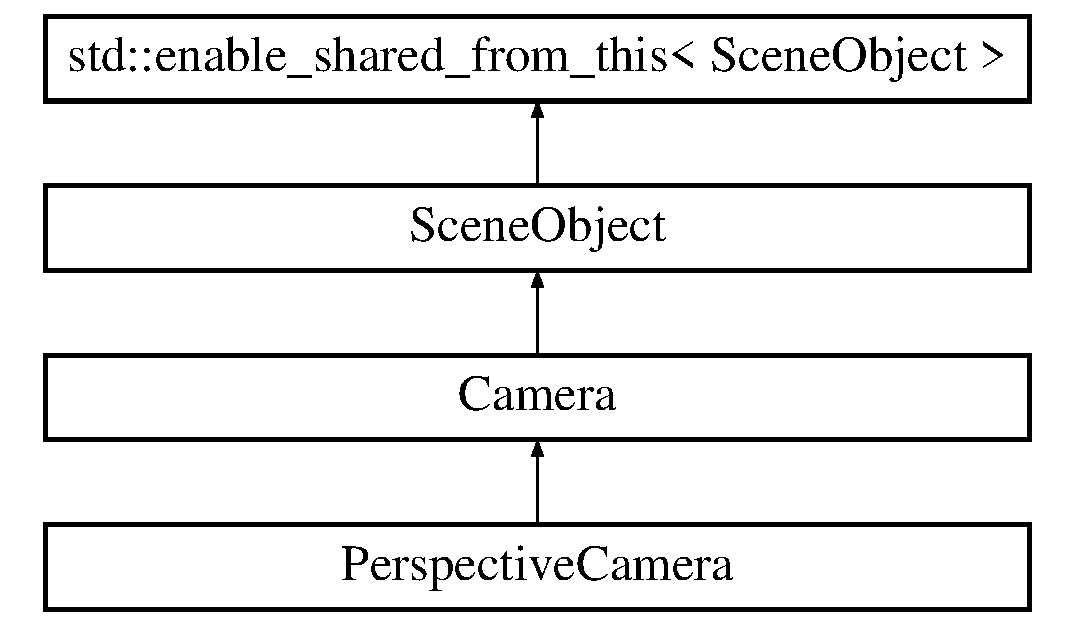
\includegraphics[height=4.000000cm]{class_camera}
\end{center}
\end{figure}
\subsection*{Public Member Functions}
\begin{DoxyCompactItemize}
\item
\hyperlink{class_camera_a01f94c3543f56ede7af49dc778f19331}{Camera} ()
\begin{DoxyCompactList}\small\item\em Creates the default camera. \end{DoxyCompactList}\item
virtual glm\+::mat4 \hyperlink{class_camera_af6f4415189deaff158ba86f0b3527a30}{Get\+Projection\+Matrix} () const
\begin{DoxyCompactList}\small\item\em Creates the projection matrix. \end{DoxyCompactList}\end{DoxyCompactItemize}
\subsection*{Protected Member Functions}
\begin{DoxyCompactItemize}
\item
virtual void \hyperlink{class_camera_aea640c892a3807671d8ca49616d96eda}{Update\+Transformation\+Matrix} ()
\begin{DoxyCompactList}\small\item\em Override the \hyperlink{class_scene_object_a20e31da3f9d2765de50cdb2d637ae6c9}{Scene\+Object\+::\+Update\+Transformation\+Matrix()} to do nothing. \end{DoxyCompactList}\end{DoxyCompactItemize}
\subsection*{Additional Inherited Members}


\subsection{Detailed Description}
The camera interface that also serves as a \char`\"{}null\char`\"{} camera.

If you use the \hyperlink{class_camera}{Camera} class directly, it will apply no transformations (aka the projection and view matrices will be the identity matrix) so you will be working with in normalized device coordinates.

\subsection{Constructor \& Destructor Documentation}
\hypertarget{class_camera_a01f94c3543f56ede7af49dc778f19331}{}\label{class_camera_a01f94c3543f56ede7af49dc778f19331}
\index{Camera@{Camera}!Camera@{Camera}}
\index{Camera@{Camera}!Camera@{Camera}}
\subsubsection{\texorpdfstring{Camera()}{Camera()}}
{\footnotesize\ttfamily Camera\+::\+Camera (\begin{DoxyParamCaption}{ }\end{DoxyParamCaption})}



Creates the default camera.



\subsection{Member Function Documentation}
\hypertarget{class_camera_af6f4415189deaff158ba86f0b3527a30}{}\label{class_camera_af6f4415189deaff158ba86f0b3527a30}
\index{Camera@{Camera}!Get\+Projection\+Matrix@{Get\+Projection\+Matrix}}
\index{Get\+Projection\+Matrix@{Get\+Projection\+Matrix}!Camera@{Camera}}
\subsubsection{\texorpdfstring{Get\+Projection\+Matrix()}{GetProjectionMatrix()}}
{\footnotesize\ttfamily glm\+::mat4 Camera\+::\+Get\+Projection\+Matrix (\begin{DoxyParamCaption}{ }\end{DoxyParamCaption}) const\hspace{0.3cm}{\ttfamily [virtual]}}



Creates the projection matrix.

\begin{DoxyReturn}{Returns}
The identity matrix.
\end{DoxyReturn}
This matrix will be the \char`\"{}\+P\char`\"{} in the M\+VP matrices.

Reimplemented in \hyperlink{class_perspective_camera_ab467388c7d3e4c2ef9b498c16f291545}{Perspective\+Camera}.

\hypertarget{class_camera_aea640c892a3807671d8ca49616d96eda}{}\label{class_camera_aea640c892a3807671d8ca49616d96eda}
\index{Camera@{Camera}!Update\+Transformation\+Matrix@{Update\+Transformation\+Matrix}}
\index{Update\+Transformation\+Matrix@{Update\+Transformation\+Matrix}!Camera@{Camera}}
\subsubsection{\texorpdfstring{Update\+Transformation\+Matrix()}{UpdateTransformationMatrix()}}
{\footnotesize\ttfamily void Camera\+::\+Update\+Transformation\+Matrix (\begin{DoxyParamCaption}{ }\end{DoxyParamCaption})\hspace{0.3cm}{\ttfamily [protected]}, {\ttfamily [virtual]}}



Override the \hyperlink{class_scene_object_a20e31da3f9d2765de50cdb2d637ae6c9}{Scene\+Object\+::\+Update\+Transformation\+Matrix()} to do nothing.

This will guarantee that the transformation matrix will always be an identity matrix regardless of whether you move/rotate/scale the camera.

Reimplemented from \hyperlink{class_scene_object_a20e31da3f9d2765de50cdb2d637ae6c9}{Scene\+Object}.



Reimplemented in \hyperlink{class_perspective_camera_a2f17fb07425e2146d5692805753fa368}{Perspective\+Camera}.



The documentation for this class was generated from the following files\+:\begin{DoxyCompactItemize}
\item
/data/MO814A-MC937A/MO814A-MC937Aopengl-\/instructor/source/common/\+Scene/\+Camera/\hyperlink{_camera_8h}{Camera.\+h}\item
/data/MO814A-MC937A/MO814A-MC937Aopengl-\/instructor/source/common/\+Scene/\+Camera/\hyperlink{_camera_8cpp}{Camera.\+cpp}\end{DoxyCompactItemize}

\hypertarget{class_cube_map_shader}{}\section{Cube\+Map\+Shader Class Reference}
\label{class_cube_map_shader}\index{Cube\+Map\+Shader@{Cube\+Map\+Shader}}


{\ttfamily \#include $<$Cube\+Map\+Shader.\+h$>$}

Inheritance diagram for Cube\+Map\+Shader\+:\begin{figure}[H]
\begin{center}
\leavevmode
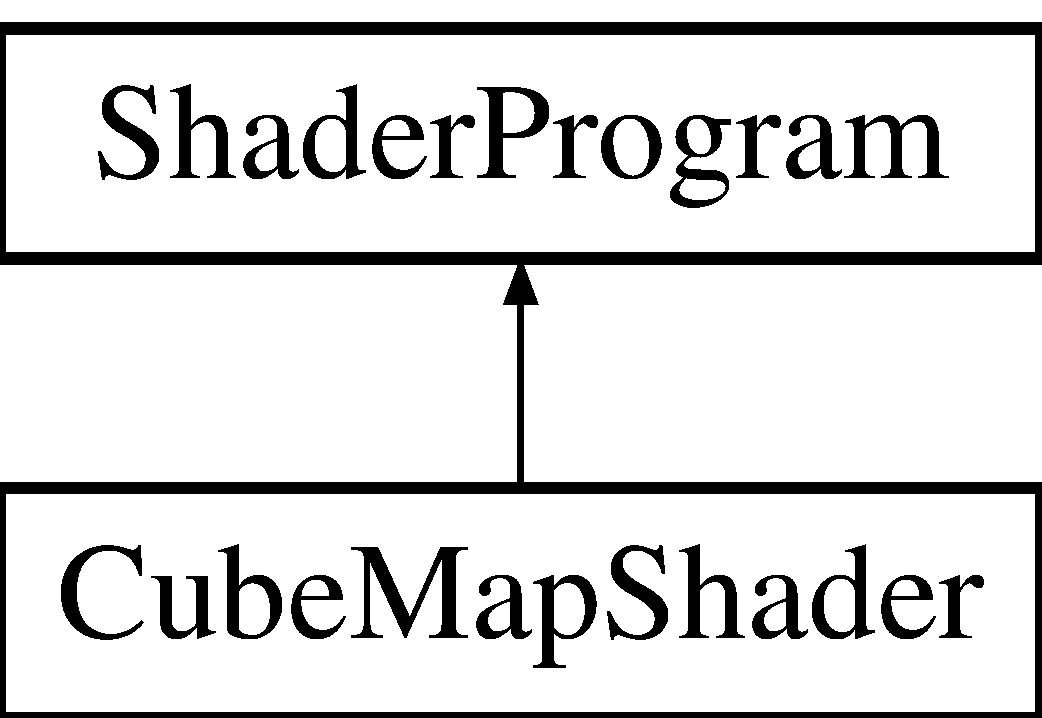
\includegraphics[height=2.000000cm]{class_cube_map_shader}
\end{center}
\end{figure}
\subsection*{Public Member Functions}
\begin{DoxyCompactItemize}
\item
\hyperlink{class_cube_map_shader_abfd5fb870087965ef8d37323f7f9ed3a}{Cube\+Map\+Shader} (const std\+::unordered\+\_\+map$<$ G\+Lenum, std\+::string $>$ \&input\+Shaders, std\+::shared\+\_\+ptr$<$ class \hyperlink{class_cube_map_texture}{Cube\+Map\+Texture} $>$ input\+Texture)
\item
virtual void \hyperlink{class_cube_map_shader_a9deaf42646258af9237751f331fb215a}{Setup\+Shader\+Materials} () const
\begin{DoxyCompactList}\small\item\em Sets up the shader material (what this material is depends on the shader). \end{DoxyCompactList}\item
virtual bool \hyperlink{class_cube_map_shader_aa0c9e535cb18663acd9857165abc788f}{Is\+Affected\+By\+Light} (const class \hyperlink{class_light}{Light} $\ast$light) const
\end{DoxyCompactItemize}
\subsection*{Private Attributes}
\begin{DoxyCompactItemize}
\item
std\+::shared\+\_\+ptr$<$ class \hyperlink{class_cube_map_texture}{Cube\+Map\+Texture} $>$ \hyperlink{class_cube_map_shader_ab9ea944d2b14c6a47406e36d9046caa6}{env\+Map}
\end{DoxyCompactItemize}
\subsection*{Additional Inherited Members}


\subsection{Constructor \& Destructor Documentation}
\hypertarget{class_cube_map_shader_abfd5fb870087965ef8d37323f7f9ed3a}{}\label{class_cube_map_shader_abfd5fb870087965ef8d37323f7f9ed3a}
\index{Cube\+Map\+Shader@{Cube\+Map\+Shader}!Cube\+Map\+Shader@{Cube\+Map\+Shader}}
\index{Cube\+Map\+Shader@{Cube\+Map\+Shader}!Cube\+Map\+Shader@{Cube\+Map\+Shader}}
\subsubsection{\texorpdfstring{Cube\+Map\+Shader()}{CubeMapShader()}}
{\footnotesize\ttfamily Cube\+Map\+Shader\+::\+Cube\+Map\+Shader (\begin{DoxyParamCaption}\item[{const std\+::unordered\+\_\+map$<$ G\+Lenum, std\+::string $>$ \&}]{input\+Shaders,  }\item[{std\+::shared\+\_\+ptr$<$ class \hyperlink{class_cube_map_texture}{Cube\+Map\+Texture} $>$}]{input\+Texture }\end{DoxyParamCaption})}



\subsection{Member Function Documentation}
\hypertarget{class_cube_map_shader_aa0c9e535cb18663acd9857165abc788f}{}\label{class_cube_map_shader_aa0c9e535cb18663acd9857165abc788f}
\index{Cube\+Map\+Shader@{Cube\+Map\+Shader}!Is\+Affected\+By\+Light@{Is\+Affected\+By\+Light}}
\index{Is\+Affected\+By\+Light@{Is\+Affected\+By\+Light}!Cube\+Map\+Shader@{Cube\+Map\+Shader}}
\subsubsection{\texorpdfstring{Is\+Affected\+By\+Light()}{IsAffectedByLight()}}
{\footnotesize\ttfamily bool Cube\+Map\+Shader\+::\+Is\+Affected\+By\+Light (\begin{DoxyParamCaption}\item[{const class \hyperlink{class_light}{Light} $\ast$}]{light }\end{DoxyParamCaption}) const\hspace{0.3cm}{\ttfamily [virtual]}}



Reimplemented from \hyperlink{class_shader_program_a20b5ed7b5f81154025eb7b6f1be70f84}{Shader\+Program}.

\hypertarget{class_cube_map_shader_a9deaf42646258af9237751f331fb215a}{}\label{class_cube_map_shader_a9deaf42646258af9237751f331fb215a}
\index{Cube\+Map\+Shader@{Cube\+Map\+Shader}!Setup\+Shader\+Materials@{Setup\+Shader\+Materials}}
\index{Setup\+Shader\+Materials@{Setup\+Shader\+Materials}!Cube\+Map\+Shader@{Cube\+Map\+Shader}}
\subsubsection{\texorpdfstring{Setup\+Shader\+Materials()}{SetupShaderMaterials()}}
{\footnotesize\ttfamily void Cube\+Map\+Shader\+::\+Setup\+Shader\+Materials (\begin{DoxyParamCaption}{ }\end{DoxyParamCaption}) const\hspace{0.3cm}{\ttfamily [virtual]}}



Sets up the shader material (what this material is depends on the shader).

This functions is meant to be a general setup function for the shader. This function has no access to the scene or anything else stored in the application so its primary purpose is to work with objects stored within the shader program object (i.\+e. textures).

Reimplemented from \hyperlink{class_shader_program_a20ea5669f122fa6143e7fa8ee9d92578}{Shader\+Program}.



\subsection{Member Data Documentation}
\hypertarget{class_cube_map_shader_ab9ea944d2b14c6a47406e36d9046caa6}{}\label{class_cube_map_shader_ab9ea944d2b14c6a47406e36d9046caa6}
\index{Cube\+Map\+Shader@{Cube\+Map\+Shader}!env\+Map@{env\+Map}}
\index{env\+Map@{env\+Map}!Cube\+Map\+Shader@{Cube\+Map\+Shader}}
\subsubsection{\texorpdfstring{env\+Map}{envMap}}
{\footnotesize\ttfamily std\+::shared\+\_\+ptr$<$class \hyperlink{class_cube_map_texture}{Cube\+Map\+Texture}$>$ Cube\+Map\+Shader\+::env\+Map\hspace{0.3cm}{\ttfamily [private]}}



The documentation for this class was generated from the following files\+:\begin{DoxyCompactItemize}
\item
/data/MO814A-MC937A/MO814A-MC937Aopengl-\/instructor/source/common/\+Rendering/\+Shaders/\hyperlink{_cube_map_shader_8h}{Cube\+Map\+Shader.\+h}\item
/data/MO814A-MC937A/MO814A-MC937Aopengl-\/instructor/source/common/\+Rendering/\+Shaders/\hyperlink{_cube_map_shader_8cpp}{Cube\+Map\+Shader.\+cpp}\end{DoxyCompactItemize}

\hypertarget{class_cube_map_texture}{}\section{Cube\+Map\+Texture Class Reference}
\label{class_cube_map_texture}\index{Cube\+Map\+Texture@{Cube\+Map\+Texture}}


{\ttfamily \#include $<$Cube\+Map\+Texture.\+h$>$}

Inheritance diagram for Cube\+Map\+Texture\+:\begin{figure}[H]
\begin{center}
\leavevmode
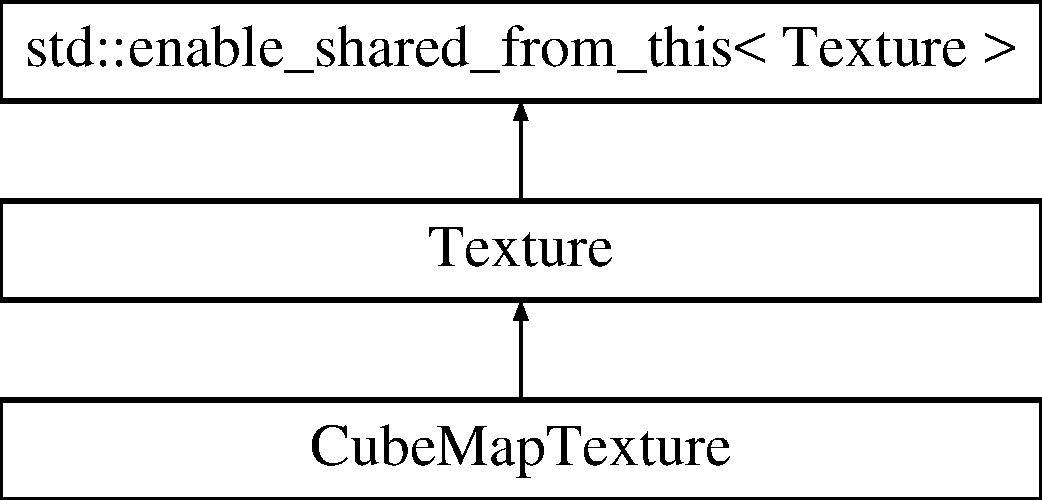
\includegraphics[height=3.000000cm]{class_cube_map_texture}
\end{center}
\end{figure}
\subsection*{Public Member Functions}
\begin{DoxyCompactItemize}
\item
\hyperlink{class_cube_map_texture_adf0b01d1180ddc452ed1cf02bf5f7687}{Cube\+Map\+Texture} (G\+Lubyte $\ast$data\mbox{[}6\mbox{]}, int width, int height)
\end{DoxyCompactItemize}
\subsection*{Private Attributes}
\begin{DoxyCompactItemize}
\item
int \hyperlink{class_cube_map_texture_a7890234be6ca631a5f17a9ab9d7e597c}{tex\+Width}
\item
int \hyperlink{class_cube_map_texture_ad7cb6fe0f1405749dac36016772b4de9}{tex\+Height}
\end{DoxyCompactItemize}
\subsection*{Additional Inherited Members}


\subsection{Constructor \& Destructor Documentation}
\hypertarget{class_cube_map_texture_adf0b01d1180ddc452ed1cf02bf5f7687}{}\label{class_cube_map_texture_adf0b01d1180ddc452ed1cf02bf5f7687}
\index{Cube\+Map\+Texture@{Cube\+Map\+Texture}!Cube\+Map\+Texture@{Cube\+Map\+Texture}}
\index{Cube\+Map\+Texture@{Cube\+Map\+Texture}!Cube\+Map\+Texture@{Cube\+Map\+Texture}}
\subsubsection{\texorpdfstring{Cube\+Map\+Texture()}{CubeMapTexture()}}
{\footnotesize\ttfamily Cube\+Map\+Texture\+::\+Cube\+Map\+Texture (\begin{DoxyParamCaption}\item[{G\+Lubyte $\ast$}]{data\mbox{[}6\mbox{]},  }\item[{int}]{width,  }\item[{int}]{height }\end{DoxyParamCaption})}



\subsection{Member Data Documentation}
\hypertarget{class_cube_map_texture_ad7cb6fe0f1405749dac36016772b4de9}{}\label{class_cube_map_texture_ad7cb6fe0f1405749dac36016772b4de9}
\index{Cube\+Map\+Texture@{Cube\+Map\+Texture}!tex\+Height@{tex\+Height}}
\index{tex\+Height@{tex\+Height}!Cube\+Map\+Texture@{Cube\+Map\+Texture}}
\subsubsection{\texorpdfstring{tex\+Height}{texHeight}}
{\footnotesize\ttfamily int Cube\+Map\+Texture\+::tex\+Height\hspace{0.3cm}{\ttfamily [private]}}

\hypertarget{class_cube_map_texture_a7890234be6ca631a5f17a9ab9d7e597c}{}\label{class_cube_map_texture_a7890234be6ca631a5f17a9ab9d7e597c}
\index{Cube\+Map\+Texture@{Cube\+Map\+Texture}!tex\+Width@{tex\+Width}}
\index{tex\+Width@{tex\+Width}!Cube\+Map\+Texture@{Cube\+Map\+Texture}}
\subsubsection{\texorpdfstring{tex\+Width}{texWidth}}
{\footnotesize\ttfamily int Cube\+Map\+Texture\+::tex\+Width\hspace{0.3cm}{\ttfamily [private]}}



The documentation for this class was generated from the following files\+:\begin{DoxyCompactItemize}
\item
/data/MO814A-MC937A/MO814A-MC937Aopengl-\/instructor/source/common/\+Rendering/\+Textures/\hyperlink{_cube_map_texture_8h}{Cube\+Map\+Texture.\+h}\item
/data/MO814A-MC937A/MO814A-MC937Aopengl-\/instructor/source/common/\+Rendering/\+Textures/\hyperlink{_cube_map_texture_8cpp}{Cube\+Map\+Texture.\+cpp}\end{DoxyCompactItemize}

\hypertarget{class_forward_renderer}{}\section{Forward\+Renderer Class Reference}
\label{class_forward_renderer}\index{Forward\+Renderer@{Forward\+Renderer}}


A multi-\/pass forward renderer with lights.




{\ttfamily \#include $<$Forward\+Renderer.\+h$>$}

Inheritance diagram for Forward\+Renderer\+:\begin{figure}[H]
\begin{center}
\leavevmode
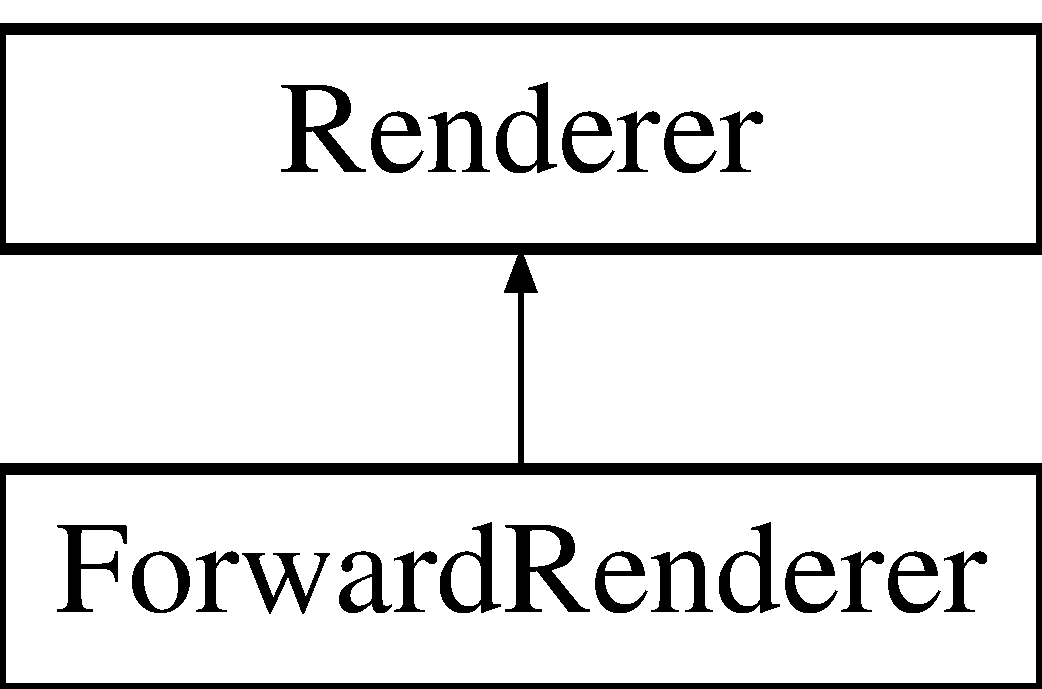
\includegraphics[height=2.000000cm]{class_forward_renderer}
\end{center}
\end{figure}
\subsection*{Public Member Functions}
\begin{DoxyCompactItemize}
\item
\hyperlink{class_forward_renderer_af8ed84e45085c4dc60d565fcc3c198d1}{Forward\+Renderer} (std\+::shared\+\_\+ptr$<$ class \hyperlink{class_scene}{Scene} $>$ input\+Scene, std\+::shared\+\_\+ptr$<$ class \hyperlink{class_camera}{Camera} $>$ input\+Camera)
\begin{DoxyCompactList}\small\item\em Stores the input scene and the input camera for use for rendering. \end{DoxyCompactList}\item
virtual \hyperlink{class_forward_renderer_ab27ea6139730631d79488cec3c564597}{$\sim$\+Forward\+Renderer} ()
\begin{DoxyCompactList}\small\item\em Just a day in the life of a destructor. \end{DoxyCompactList}\item
virtual void \hyperlink{class_forward_renderer_a5cbca647822780d6cfbd39552d73ee06}{Initialize} () override
\begin{DoxyCompactList}\small\item\em Loads the data that the forward renderer needs. \end{DoxyCompactList}\item 
virtual void \hyperlink{class_forward_renderer_a1a5deafa5deaf1e0abaab0e2074928c1}{Render} () override
\begin{DoxyCompactList}\small\item\em Renders a frame using a multi-\/pass forward renderer with all the lights in the scene. \end{DoxyCompactList}\end{DoxyCompactItemize}
\subsection*{Additional Inherited Members}


\subsection{Detailed Description}
A multi-\/pass forward renderer with lights.

More details about what a multi-\/pass forward renderer is can be found in the documentation for the \hyperlink{class_forward_renderer_a1a5deafa5deaf1e0abaab0e2074928c1}{Render()} function. Do note that this class will not support transparent objects out of the box! You will have to find a way to handle them if you want to display transparent objects properly.

\subsection{Constructor \& Destructor Documentation}
\hypertarget{class_forward_renderer_af8ed84e45085c4dc60d565fcc3c198d1}{}\label{class_forward_renderer_af8ed84e45085c4dc60d565fcc3c198d1}
\index{Forward\+Renderer@{Forward\+Renderer}!Forward\+Renderer@{Forward\+Renderer}}
\index{Forward\+Renderer@{Forward\+Renderer}!Forward\+Renderer@{Forward\+Renderer}}
\subsubsection{\texorpdfstring{Forward\+Renderer()}{ForwardRenderer()}}
{\footnotesize\ttfamily Forward\+Renderer\+::\+Forward\+Renderer (\begin{DoxyParamCaption}\item[{std\+::shared\+\_\+ptr$<$ class \hyperlink{class_scene}{Scene} $>$}]{input\+Scene,  }\item[{std\+::shared\+\_\+ptr$<$ class \hyperlink{class_camera}{Camera} $>$}]{input\+Camera }\end{DoxyParamCaption})}



Stores the input scene and the input camera for use for rendering.

Calls the base class constructor, \hyperlink{class_renderer_adc8ce31cd649bdf220ca8355809b1d06}{Renderer\+::\+Renderer()}. \hypertarget{class_forward_renderer_ab27ea6139730631d79488cec3c564597}{}\label{class_forward_renderer_ab27ea6139730631d79488cec3c564597}
\index{Forward\+Renderer@{Forward\+Renderer}!````~Forward\+Renderer@{$\sim$\+Forward\+Renderer}}
\index{````~Forward\+Renderer@{$\sim$\+Forward\+Renderer}!Forward\+Renderer@{Forward\+Renderer}}
\subsubsection{\texorpdfstring{$\sim$\+Forward\+Renderer()}{~ForwardRenderer()}}
{\footnotesize\ttfamily Forward\+Renderer\+::$\sim$\+Forward\+Renderer (\begin{DoxyParamCaption}{ }\end{DoxyParamCaption})\hspace{0.3cm}{\ttfamily [virtual]}}



Just a day in the life of a destructor.



\subsection{Member Function Documentation}
\hypertarget{class_forward_renderer_a5cbca647822780d6cfbd39552d73ee06}{}\label{class_forward_renderer_a5cbca647822780d6cfbd39552d73ee06}
\index{Forward\+Renderer@{Forward\+Renderer}!Initialize@{Initialize}}
\index{Initialize@{Initialize}!Forward\+Renderer@{Forward\+Renderer}}
\subsubsection{\texorpdfstring{Initialize()}{Initialize()}}
{\footnotesize\ttfamily void Forward\+Renderer\+::\+Initialize (\begin{DoxyParamCaption}{ }\end{DoxyParamCaption})\hspace{0.3cm}{\ttfamily [override]}, {\ttfamily [virtual]}}



Loads the data that the forward renderer needs.

Loads the depth prepass shader. See the documentation of \hyperlink{class_forward_renderer_a1a5deafa5deaf1e0abaab0e2074928c1}{Render()} for why it is necessary.

Implements \hyperlink{class_renderer_a7cb221f355f181d84d66e8c09f50f04a}{Renderer}.

\hypertarget{class_forward_renderer_a1a5deafa5deaf1e0abaab0e2074928c1}{}\label{class_forward_renderer_a1a5deafa5deaf1e0abaab0e2074928c1}
\index{Forward\+Renderer@{Forward\+Renderer}!Render@{Render}}
\index{Render@{Render}!Forward\+Renderer@{Forward\+Renderer}}
\subsubsection{\texorpdfstring{Render()}{Render()}}
{\footnotesize\ttfamily void Forward\+Renderer\+::\+Render (\begin{DoxyParamCaption}{ }\end{DoxyParamCaption})\hspace{0.3cm}{\ttfamily [override]}, {\ttfamily [virtual]}}



Renders a frame using a multi-\/pass forward renderer with all the lights in the scene.

Note that in the multi-\/pass forward renderer, there is no limit to how many lights you may use; however, once the number of lights becomes too high, you will start to see a significant drop in frames per second. In our implementation of the multi-\/pass forward renderer, assuming that there are $N$ lights, the renderer will perform $ N + 2 $ passes through every object in the scene. For every draw call, the multi-\/pass forward renderer will perform additive blending of both the R\+GB and alpha channels to compute the new color in the color buffer. The render pass stages are as follows\+:


\begin{DoxyEnumerate}
\item The depth preprocess stage. Without this stage, some objects will transparent even if they are not actually. Let\textquotesingle{}s say a relative large and complex object has parts that are facing towards the camera but are occluded. Then let\textquotesingle{}s say that the light vertex/fragment shader processes that part first and then processes the occluder parts later. With additive blending turned on, the colors will be mixed! Turning additive blending is not an option for a multi-\/pass forward renderer. Instead what we want to do is to perform an initial \char`\"{}depth preprocess\char`\"{} pass through every object in the scene. By doing this, we write the final depth of an object to the depth buffer. In the subsequent render passes, we will only write to the color buffer is the depth value is less than or equal to the value already stored in the depth buffer. Since we ran the depth preprocess pass on E\+V\+E\+RY object in the scene, we are guaranteed that the value stored in the depth buffer is the smallest possible value for that pixel. So if a render pass passes the depth buffer check, it can know for sure that it is safe to write to the color buffer and that there won\textquotesingle{}t be another object occluding it. It is important to note that depth is stored as a floating point value and with floating point values comes numerical imprecision which can result in \href{https://en.wikipedia.org/wiki/Z-fighting}{\tt z-\/fighting}. As a result, we use \href{https://www.opengl.org/sdk/docs/man/html/glPolygonOffset.xhtml}{\tt gl\+Polygon\+Offset} to offset the depth values ever so slightly to prevent z-\/fighting from occurring. The amount that we offset $\sim$should$\sim$ not be enough to cause problems with fragments passing the depth buffer test that otherwise should not.
\item The \char`\"{}global lighting\char`\"{} phase. This phase takes care of the ambient color of the material (Note\+: it might make more sense for the ambient color be a property of the light and not the material). Regardless, this phase will take care of the color that should only be added to the object once regardless of how many lights shine upon it. Good examples of things that would go in this stage are the ambient and emissive colors.
\item Finally, the rest of the lighting passes are dedicated to performing a normal render pass with a light in the scene. The rendering object in question is queried for the correct shader to use, the shader is then setup by the rendering object and the scene object, and finally the object is rendered and the resulting fragment colors are correctly blended into the color buffer.
\end{DoxyEnumerate}

Still confused? Ask on Piazza!

Implements \hyperlink{class_renderer_a38623da22aa718cfa41e2514ebd269f5}{Renderer}.



The documentation for this class was generated from the following files\+:\begin{DoxyCompactItemize}
\item
/data/MO814A-MC937A/MO814A-MC937Aopengl-\/instructor/source/common/\+Rendering/\hyperlink{_forward_renderer_8h}{Forward\+Renderer.\+h}\item
/data/MO814A-MC937A/MO814A-MC937Aopengl-\/instructor/source/common/\+Rendering/\hyperlink{_forward_renderer_8cpp}{Forward\+Renderer.\+cpp}\end{DoxyCompactItemize}

\hypertarget{class_light}{}\section{Light Class Reference}
\label{class_light}\index{Light@{Light}}


Generic light class.




{\ttfamily \#include $<$Light.\+h$>$}

Inheritance diagram for Light\+:\begin{figure}[H]
\begin{center}
\leavevmode
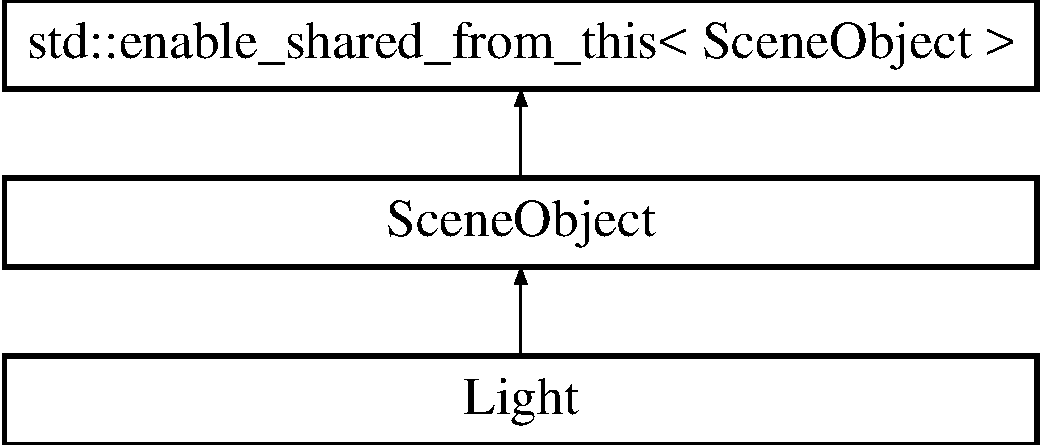
\includegraphics[height=3.000000cm]{class_light}
\end{center}
\end{figure}
\subsection*{Public Types}
\begin{DoxyCompactItemize}
\item 
enum \hyperlink{class_light_a661d9480e01af8b1612860b9630ef5f8}{Light\+Type} \{ \newline
\hyperlink{class_light_a661d9480e01af8b1612860b9630ef5f8a6eecfba72d12922ee1dead07a0ef3334}{Light\+Type\+::\+G\+L\+O\+B\+AL} = 0,
\hyperlink{class_light_a661d9480e01af8b1612860b9630ef5f8aaebdbcb765394d25d6a604589a890f82}{Light\+Type\+::\+P\+O\+I\+NT},
\hyperlink{class_light_a661d9480e01af8b1612860b9630ef5f8ab6f2249394a4def60a78b342dcc925b9}{Light\+Type\+::\+D\+I\+R\+E\+C\+T\+I\+O\+N\+AL},
\hyperlink{class_light_a661d9480e01af8b1612860b9630ef5f8a745727a64f32080cf213b668026dde48}{Light\+Type\+::\+H\+E\+M\+I\+S\+P\+H\+E\+RE},
\newline
\hyperlink{class_light_a661d9480e01af8b1612860b9630ef5f8a239e71da0606abd283f2bccf1965badd}{Light\+Type\+::\+I\+BL}
 \}\begin{DoxyCompactList}\small\item\em The different types of light. \end{DoxyCompactList}
\end{DoxyCompactItemize}
\subsection*{Public Member Functions}
\begin{DoxyCompactItemize}
\item
\hyperlink{class_light_adca12f0d5470bc3f2e6e77233ab3dcf1}{Light} (std\+::unique\+\_\+ptr$<$ struct \hyperlink{struct_light_properties}{Light\+Properties} $>$ in\+Properties, \hyperlink{class_light_a661d9480e01af8b1612860b9630ef5f8}{Light\+Type} type=\hyperlink{class_light_a661d9480e01af8b1612860b9630ef5f8aaebdbcb765394d25d6a604589a890f82}{Light\+Type\+::\+P\+O\+I\+NT})
\begin{DoxyCompactList}\small\item\em Constructs a light from user-\/specified properties and a light type. \end{DoxyCompactList}\item
virtual \hyperlink{class_light_ad0e59fad13bb6cfadc25b2c477e9ddc7}{$\sim$\+Light} ()
\item
void \hyperlink{class_light_acd1a8b84fbcc1ef2dc8b3bc5ecf76c7b}{Get\+Attenuation} (float \&constant, float \&linear, float \&quadratic) const
\begin{DoxyCompactList}\small\item\em Returns the attenuation parameters for the light. \end{DoxyCompactList}\item
void \hyperlink{class_light_aec7f3864e328bc9fada51fdb3e8a7c8e}{Set\+Constant\+Attenuation} (float in\+Value)
\item
void \hyperlink{class_light_aa33086ed4bff3ac95c700698b3070108}{Set\+Linear\+Attenuation} (float in\+Value)
\item
void \hyperlink{class_light_a413e0445d66742c666114dd74d689fc6}{Set\+Quadratic\+Attenuation} (float in\+Value)
\item
\hyperlink{class_light_a661d9480e01af8b1612860b9630ef5f8}{Light\+Type} \hyperlink{class_light_aaa0ba2164adcab55ed7bc1f957fa1f75}{Get\+Light\+Type} () const
\item
const struct \hyperlink{struct_light_properties}{Light\+Properties} $\ast$ \hyperlink{class_light_a1d2283dacdef30df671d55b7dc415851}{Get\+Properties\+Raw} () const
\item
virtual void \hyperlink{class_light_adb3750e44ae24fefa1f4c89f933b2677}{Setup\+Shader\+Uniforms} (const class \hyperlink{class_shader_program}{Shader\+Program} $\ast$program) const
\begin{DoxyCompactList}\small\item\em Sets up the shader to have the necessary properties for a given type of light. \end{DoxyCompactList}\end{DoxyCompactItemize}
\subsection*{Private Attributes}
\begin{DoxyCompactItemize}
\item
std\+::unique\+\_\+ptr$<$ struct \hyperlink{struct_light_properties}{Light\+Properties} $>$ \hyperlink{class_light_a74eba4cac1cc27e741230fbda32fceef}{properties}
\item
\hyperlink{class_light_a661d9480e01af8b1612860b9630ef5f8}{Light\+Type} \hyperlink{class_light_ab0c279c927973443f7b52fc924b489aa}{light\+Type}
\item
float \hyperlink{class_light_afef6c00a21aa16dc6cc7a7fb1639d2fa}{constant\+Attenuation}
\item
float \hyperlink{class_light_afcb2da592197efae015ae16c1c5bfceb}{linear\+Attenuation}
\item
float \hyperlink{class_light_a0f24dde11cbbd12d0f0309e189f3640c}{quadratic\+Attenuation}
\end{DoxyCompactItemize}
\subsection*{Static Private Attributes}
\begin{DoxyCompactItemize}
\item
static const std\+::string \hyperlink{class_light_ab2d40f6c364cf728d03a90ff885e37cb}{L\+I\+G\+H\+T\+\_\+\+U\+N\+I\+F\+O\+R\+M\+\_\+\+N\+A\+ME} = \char`\"{}point\+Light\char`\"{}
\end{DoxyCompactItemize}
\subsection*{Additional Inherited Members}


\subsection{Detailed Description}
Generic light class.

Note that the \char`\"{}\+Light\char`\"{} class only holds the properties related to the orientation and shape of the camera in world space. The actual \char`\"{}light\char`\"{} of the \hyperlink{class_light}{Light} object is stored within a \hyperlink{struct_light_properties}{Light\+Properties} structure. The \hyperlink{class_light}{Light} class acts as a point light.

\subsection{Member Enumeration Documentation}
\hypertarget{class_light_a661d9480e01af8b1612860b9630ef5f8}{}\label{class_light_a661d9480e01af8b1612860b9630ef5f8}
\index{Light@{Light}!Light\+Type@{Light\+Type}}
\index{Light\+Type@{Light\+Type}!Light@{Light}}
\subsubsection{\texorpdfstring{Light\+Type}{LightType}}
{\footnotesize\ttfamily enum \hyperlink{class_light_a661d9480e01af8b1612860b9630ef5f8}{Light\+::\+Light\+Type}\hspace{0.3cm}{\ttfamily [strong]}}



The different types of light.

If you ever want to create a new type of light, you should add a new entry into the Light\+Type enum and then have the \hyperlink{class_shader_program}{Shader\+Program} subclass handle that Light\+Type properly. Note that the \hyperlink{class_light_a661d9480e01af8b1612860b9630ef5f8a6eecfba72d12922ee1dead07a0ef3334}{Light\+Type\+::\+G\+L\+O\+B\+AL} enum is used by the \hyperlink{class_blinn_phong_shader}{Blinn\+Phong\+Shader} to handle global light (if any). You can ignore this if your shader does not have any global light that should only be applied once per object. \begin{DoxyEnumFields}{Enumerator}
\raisebox{\heightof{T}}[0pt][0pt]{\index{G\+L\+O\+B\+AL@{G\+L\+O\+B\+AL}!Light@{Light}}\index{Light@{Light}!G\+L\+O\+B\+AL@{G\+L\+O\+B\+AL}}}\hypertarget{class_light_a661d9480e01af8b1612860b9630ef5f8a6eecfba72d12922ee1dead07a0ef3334}{}\label{class_light_a661d9480e01af8b1612860b9630ef5f8a6eecfba72d12922ee1dead07a0ef3334}
G\+L\+O\+B\+AL&\\
\hline

\raisebox{\heightof{T}}[0pt][0pt]{\index{P\+O\+I\+NT@{P\+O\+I\+NT}!Light@{Light}}\index{Light@{Light}!P\+O\+I\+NT@{P\+O\+I\+NT}}}\hypertarget{class_light_a661d9480e01af8b1612860b9630ef5f8aaebdbcb765394d25d6a604589a890f82}{}\label{class_light_a661d9480e01af8b1612860b9630ef5f8aaebdbcb765394d25d6a604589a890f82}
P\+O\+I\+NT&\\
\hline

\raisebox{\heightof{T}}[0pt][0pt]{\index{D\+I\+R\+E\+C\+T\+I\+O\+N\+AL@{D\+I\+R\+E\+C\+T\+I\+O\+N\+AL}!Light@{Light}}\index{Light@{Light}!D\+I\+R\+E\+C\+T\+I\+O\+N\+AL@{D\+I\+R\+E\+C\+T\+I\+O\+N\+AL}}}\hypertarget{class_light_a661d9480e01af8b1612860b9630ef5f8ab6f2249394a4def60a78b342dcc925b9}{}\label{class_light_a661d9480e01af8b1612860b9630ef5f8ab6f2249394a4def60a78b342dcc925b9}
D\+I\+R\+E\+C\+T\+I\+O\+N\+AL&\\
\hline

\raisebox{\heightof{T}}[0pt][0pt]{\index{H\+E\+M\+I\+S\+P\+H\+E\+RE@{H\+E\+M\+I\+S\+P\+H\+E\+RE}!Light@{Light}}\index{Light@{Light}!H\+E\+M\+I\+S\+P\+H\+E\+RE@{H\+E\+M\+I\+S\+P\+H\+E\+RE}}}\hypertarget{class_light_a661d9480e01af8b1612860b9630ef5f8a745727a64f32080cf213b668026dde48}{}\label{class_light_a661d9480e01af8b1612860b9630ef5f8a745727a64f32080cf213b668026dde48}
H\+E\+M\+I\+S\+P\+H\+E\+RE&\\
\hline

\raisebox{\heightof{T}}[0pt][0pt]{\index{I\+BL@{I\+BL}!Light@{Light}}\index{Light@{Light}!I\+BL@{I\+BL}}}\hypertarget{class_light_a661d9480e01af8b1612860b9630ef5f8a239e71da0606abd283f2bccf1965badd}{}\label{class_light_a661d9480e01af8b1612860b9630ef5f8a239e71da0606abd283f2bccf1965badd}
I\+BL&\\
\hline

\end{DoxyEnumFields}


\subsection{Constructor \& Destructor Documentation}
\hypertarget{class_light_adca12f0d5470bc3f2e6e77233ab3dcf1}{}\label{class_light_adca12f0d5470bc3f2e6e77233ab3dcf1}
\index{Light@{Light}!Light@{Light}}
\index{Light@{Light}!Light@{Light}}
\subsubsection{\texorpdfstring{Light()}{Light()}}
{\footnotesize\ttfamily Light\+::\+Light (\begin{DoxyParamCaption}\item[{std\+::unique\+\_\+ptr$<$ struct \hyperlink{struct_light_properties}{Light\+Properties} $>$}]{in\+Properties,  }\item[{\hyperlink{class_light_a661d9480e01af8b1612860b9630ef5f8}{Light\+Type}}]{type = {\ttfamily \hyperlink{class_light_a661d9480e01af8b1612860b9630ef5f8aaebdbcb765394d25d6a604589a890f82}{Light\+Type\+::\+P\+O\+I\+NT}} }\end{DoxyParamCaption})}



Constructs a light from user-\/specified properties and a light type.


\begin{DoxyParams}{Parameters}
{\em in\+Properties} & The \hyperlink{struct_light_properties}{Light\+Properties} structure. The type of this property is dependent on what shader is being used. \\
\hline
{\em type} & The type of light as enumerated in the Light\+Type enum.\\
\hline
\end{DoxyParams}
Subclasses of the \hyperlink{class_light}{Light} class should pass in the appropriate Light\+Type to the base class constructor. Note that a point light should probably be its own subclass instead of just hijacking the base class. \hypertarget{class_light_ad0e59fad13bb6cfadc25b2c477e9ddc7}{}\label{class_light_ad0e59fad13bb6cfadc25b2c477e9ddc7}
\index{Light@{Light}!````~Light@{$\sim$\+Light}}
\index{````~Light@{$\sim$\+Light}!Light@{Light}}
\subsubsection{\texorpdfstring{$\sim$\+Light()}{~Light()}}
{\footnotesize\ttfamily Light\+::$\sim$\+Light (\begin{DoxyParamCaption}{ }\end{DoxyParamCaption})\hspace{0.3cm}{\ttfamily [virtual]}}



\subsection{Member Function Documentation}
\hypertarget{class_light_acd1a8b84fbcc1ef2dc8b3bc5ecf76c7b}{}\label{class_light_acd1a8b84fbcc1ef2dc8b3bc5ecf76c7b}
\index{Light@{Light}!Get\+Attenuation@{Get\+Attenuation}}
\index{Get\+Attenuation@{Get\+Attenuation}!Light@{Light}}
\subsubsection{\texorpdfstring{Get\+Attenuation()}{GetAttenuation()}}
{\footnotesize\ttfamily void Light\+::\+Get\+Attenuation (\begin{DoxyParamCaption}\item[{float \&}]{constant,  }\item[{float \&}]{linear,  }\item[{float \&}]{quadratic }\end{DoxyParamCaption}) const}



Returns the attenuation parameters for the light.


\begin{DoxyParams}{Parameters}
{\em constant} & Reference where the constant attenuation will be written to. \\
\hline
{\em linear} & Reference where the linear attenuation will be written to. \\
\hline
{\em quadratic} & Reference where the quadratic attenuation will be written to.\\
\hline
\end{DoxyParams}
Let us define $d$ as the distance a vertex is from the light. Furthermore, let\textquotesingle{}s define $c$ as the constant attenuation, $l$ as the linear attenuation, and $q$ as the quadratic attenuation. Then the light\textquotesingle{}s intensity will be multiplied by $\frac{1}{c + d l + d^2 l}$. \hypertarget{class_light_aaa0ba2164adcab55ed7bc1f957fa1f75}{}\label{class_light_aaa0ba2164adcab55ed7bc1f957fa1f75}
\index{Light@{Light}!Get\+Light\+Type@{Get\+Light\+Type}}
\index{Get\+Light\+Type@{Get\+Light\+Type}!Light@{Light}}
\subsubsection{\texorpdfstring{Get\+Light\+Type()}{GetLightType()}}
{\footnotesize\ttfamily \hyperlink{class_light_a661d9480e01af8b1612860b9630ef5f8}{Light\+Type} Light\+::\+Get\+Light\+Type (\begin{DoxyParamCaption}{ }\end{DoxyParamCaption}) const\hspace{0.3cm}{\ttfamily [inline]}}

\hypertarget{class_light_a1d2283dacdef30df671d55b7dc415851}{}\label{class_light_a1d2283dacdef30df671d55b7dc415851}
\index{Light@{Light}!Get\+Properties\+Raw@{Get\+Properties\+Raw}}
\index{Get\+Properties\+Raw@{Get\+Properties\+Raw}!Light@{Light}}
\subsubsection{\texorpdfstring{Get\+Properties\+Raw()}{GetPropertiesRaw()}}
{\footnotesize\ttfamily const \hyperlink{struct_light_properties}{Light\+Properties} $\ast$ Light\+::\+Get\+Properties\+Raw (\begin{DoxyParamCaption}{ }\end{DoxyParamCaption}) const}

\hypertarget{class_light_aec7f3864e328bc9fada51fdb3e8a7c8e}{}\label{class_light_aec7f3864e328bc9fada51fdb3e8a7c8e}
\index{Light@{Light}!Set\+Constant\+Attenuation@{Set\+Constant\+Attenuation}}
\index{Set\+Constant\+Attenuation@{Set\+Constant\+Attenuation}!Light@{Light}}
\subsubsection{\texorpdfstring{Set\+Constant\+Attenuation()}{SetConstantAttenuation()}}
{\footnotesize\ttfamily void Light\+::\+Set\+Constant\+Attenuation (\begin{DoxyParamCaption}\item[{float}]{in\+Value }\end{DoxyParamCaption})}

\hypertarget{class_light_aa33086ed4bff3ac95c700698b3070108}{}\label{class_light_aa33086ed4bff3ac95c700698b3070108}
\index{Light@{Light}!Set\+Linear\+Attenuation@{Set\+Linear\+Attenuation}}
\index{Set\+Linear\+Attenuation@{Set\+Linear\+Attenuation}!Light@{Light}}
\subsubsection{\texorpdfstring{Set\+Linear\+Attenuation()}{SetLinearAttenuation()}}
{\footnotesize\ttfamily void Light\+::\+Set\+Linear\+Attenuation (\begin{DoxyParamCaption}\item[{float}]{in\+Value }\end{DoxyParamCaption})}

\hypertarget{class_light_a413e0445d66742c666114dd74d689fc6}{}\label{class_light_a413e0445d66742c666114dd74d689fc6}
\index{Light@{Light}!Set\+Quadratic\+Attenuation@{Set\+Quadratic\+Attenuation}}
\index{Set\+Quadratic\+Attenuation@{Set\+Quadratic\+Attenuation}!Light@{Light}}
\subsubsection{\texorpdfstring{Set\+Quadratic\+Attenuation()}{SetQuadraticAttenuation()}}
{\footnotesize\ttfamily void Light\+::\+Set\+Quadratic\+Attenuation (\begin{DoxyParamCaption}\item[{float}]{in\+Value }\end{DoxyParamCaption})}

\hypertarget{class_light_adb3750e44ae24fefa1f4c89f933b2677}{}\label{class_light_adb3750e44ae24fefa1f4c89f933b2677}
\index{Light@{Light}!Setup\+Shader\+Uniforms@{Setup\+Shader\+Uniforms}}
\index{Setup\+Shader\+Uniforms@{Setup\+Shader\+Uniforms}!Light@{Light}}
\subsubsection{\texorpdfstring{Setup\+Shader\+Uniforms()}{SetupShaderUniforms()}}
{\footnotesize\ttfamily void Light\+::\+Setup\+Shader\+Uniforms (\begin{DoxyParamCaption}\item[{const class \hyperlink{class_shader_program}{Shader\+Program} $\ast$}]{program }\end{DoxyParamCaption}) const\hspace{0.3cm}{\ttfamily [virtual]}}



Sets up the shader to have the necessary properties for a given type of light.


\begin{DoxyParams}{Parameters}
{\em program} & The shader to setup. \\
\hline
\end{DoxyParams}
\begin{DoxyWarning}{Warning}
Deprecated.
\end{DoxyWarning}
For a point light, the only thing that is necessary is the light\textquotesingle{}s position.

\subsection{Member Data Documentation}
\hypertarget{class_light_afef6c00a21aa16dc6cc7a7fb1639d2fa}{}\label{class_light_afef6c00a21aa16dc6cc7a7fb1639d2fa}
\index{Light@{Light}!constant\+Attenuation@{constant\+Attenuation}}
\index{constant\+Attenuation@{constant\+Attenuation}!Light@{Light}}
\subsubsection{\texorpdfstring{constant\+Attenuation}{constantAttenuation}}
{\footnotesize\ttfamily float Light\+::constant\+Attenuation\hspace{0.3cm}{\ttfamily [private]}}

\hypertarget{class_light_ab2d40f6c364cf728d03a90ff885e37cb}{}\label{class_light_ab2d40f6c364cf728d03a90ff885e37cb}
\index{Light@{Light}!L\+I\+G\+H\+T\+\_\+\+U\+N\+I\+F\+O\+R\+M\+\_\+\+N\+A\+ME@{L\+I\+G\+H\+T\+\_\+\+U\+N\+I\+F\+O\+R\+M\+\_\+\+N\+A\+ME}}
\index{L\+I\+G\+H\+T\+\_\+\+U\+N\+I\+F\+O\+R\+M\+\_\+\+N\+A\+ME@{L\+I\+G\+H\+T\+\_\+\+U\+N\+I\+F\+O\+R\+M\+\_\+\+N\+A\+ME}!Light@{Light}}
\subsubsection{\texorpdfstring{L\+I\+G\+H\+T\+\_\+\+U\+N\+I\+F\+O\+R\+M\+\_\+\+N\+A\+ME}{LIGHT\_UNIFORM\_NAME}}
{\footnotesize\ttfamily const std\+::string Light\+::\+L\+I\+G\+H\+T\+\_\+\+U\+N\+I\+F\+O\+R\+M\+\_\+\+N\+A\+ME = \char`\"{}point\+Light\char`\"{}\hspace{0.3cm}{\ttfamily [static]}, {\ttfamily [private]}}

\hypertarget{class_light_ab0c279c927973443f7b52fc924b489aa}{}\label{class_light_ab0c279c927973443f7b52fc924b489aa}
\index{Light@{Light}!light\+Type@{light\+Type}}
\index{light\+Type@{light\+Type}!Light@{Light}}
\subsubsection{\texorpdfstring{light\+Type}{lightType}}
{\footnotesize\ttfamily \hyperlink{class_light_a661d9480e01af8b1612860b9630ef5f8}{Light\+Type} Light\+::light\+Type\hspace{0.3cm}{\ttfamily [private]}}

\hypertarget{class_light_afcb2da592197efae015ae16c1c5bfceb}{}\label{class_light_afcb2da592197efae015ae16c1c5bfceb}
\index{Light@{Light}!linear\+Attenuation@{linear\+Attenuation}}
\index{linear\+Attenuation@{linear\+Attenuation}!Light@{Light}}
\subsubsection{\texorpdfstring{linear\+Attenuation}{linearAttenuation}}
{\footnotesize\ttfamily float Light\+::linear\+Attenuation\hspace{0.3cm}{\ttfamily [private]}}

\hypertarget{class_light_a74eba4cac1cc27e741230fbda32fceef}{}\label{class_light_a74eba4cac1cc27e741230fbda32fceef}
\index{Light@{Light}!properties@{properties}}
\index{properties@{properties}!Light@{Light}}
\subsubsection{\texorpdfstring{properties}{properties}}
{\footnotesize\ttfamily std\+::unique\+\_\+ptr$<$struct \hyperlink{struct_light_properties}{Light\+Properties}$>$ Light\+::properties\hspace{0.3cm}{\ttfamily [private]}}

\hypertarget{class_light_a0f24dde11cbbd12d0f0309e189f3640c}{}\label{class_light_a0f24dde11cbbd12d0f0309e189f3640c}
\index{Light@{Light}!quadratic\+Attenuation@{quadratic\+Attenuation}}
\index{quadratic\+Attenuation@{quadratic\+Attenuation}!Light@{Light}}
\subsubsection{\texorpdfstring{quadratic\+Attenuation}{quadraticAttenuation}}
{\footnotesize\ttfamily float Light\+::quadratic\+Attenuation\hspace{0.3cm}{\ttfamily [private]}}



The documentation for this class was generated from the following files\+:\begin{DoxyCompactItemize}
\item
/data/MO814A-MC937A/MO814A-MC937Aopengl-\/instructor/source/common/\+Scene/\+Light/\hyperlink{_light_8h}{Light.\+h}\item
/data/MO814A-MC937A/MO814A-MC937Aopengl-\/instructor/source/common/\+Scene/\+Light/\hyperlink{_light_8cpp}{Light.\+cpp}\end{DoxyCompactItemize}

\hypertarget{struct_light_properties}{}\section{Light\+Properties Struct Reference}
\label{struct_light_properties}\index{Light\+Properties@{Light\+Properties}}


{\ttfamily \#include $<$Light\+Properties.\+h$>$}

\subsection*{Public Attributes}
\begin{DoxyCompactItemize}
\item
glm\+::vec4 \hyperlink{struct_light_properties_a3af836c1b945d14e8e11baccae2c8c9e}{diffuse\+Color}
\item
glm\+::vec4 \hyperlink{struct_light_properties_a802ad3c68cfec9c97b0de463ff6e74ac}{specular\+Color}
\end{DoxyCompactItemize}


\subsection{Member Data Documentation}
\hypertarget{struct_light_properties_a3af836c1b945d14e8e11baccae2c8c9e}{}\label{struct_light_properties_a3af836c1b945d14e8e11baccae2c8c9e}
\index{Light\+Properties@{Light\+Properties}!diffuse\+Color@{diffuse\+Color}}
\index{diffuse\+Color@{diffuse\+Color}!Light\+Properties@{Light\+Properties}}
\subsubsection{\texorpdfstring{diffuse\+Color}{diffuseColor}}
{\footnotesize\ttfamily glm\+::vec4 Light\+Properties\+::diffuse\+Color}

\hypertarget{struct_light_properties_a802ad3c68cfec9c97b0de463ff6e74ac}{}\label{struct_light_properties_a802ad3c68cfec9c97b0de463ff6e74ac}
\index{Light\+Properties@{Light\+Properties}!specular\+Color@{specular\+Color}}
\index{specular\+Color@{specular\+Color}!Light\+Properties@{Light\+Properties}}
\subsubsection{\texorpdfstring{specular\+Color}{specularColor}}
{\footnotesize\ttfamily glm\+::vec4 Light\+Properties\+::specular\+Color}



The documentation for this struct was generated from the following file\+:\begin{DoxyCompactItemize}
\item
/data/MO814A-MC937A/MO814A-MC937Aopengl-\/instructor/source/common/\+Scene/\+Light/\hyperlink{_light_properties_8h}{Light\+Properties.\+h}\end{DoxyCompactItemize}

\hypertarget{class_media_layer}{}\section{Media\+Layer Class Reference}
\label{class_media_layer}\index{Media\+Layer@{Media\+Layer}}


Class that initializes the application and makes it ready to process Open\+GL commands.




{\ttfamily \#include $<$Media\+Layer.\+h$>$}

\subsection*{Public Member Functions}
\begin{DoxyCompactItemize}
\item
\hyperlink{class_media_layer_aea3b3bc36411af90517692b110d2829a}{Media\+Layer} (std\+::unique\+\_\+ptr$<$ \hyperlink{class_application}{Application} $>$ input\+App, std\+::unique\+\_\+ptr$<$ \hyperlink{class_renderer}{Renderer} $>$ input\+Renderer)
\begin{DoxyCompactList}\small\item\em Constructs a \hyperlink{class_media_layer}{Media\+Layer} object and readies the \hyperlink{class_application}{Application} and \hyperlink{class_renderer}{Renderer} for immediate use. \end{DoxyCompactList}\item
\hyperlink{class_media_layer_a0c64e2d0a1c7b34b5457a0c57b69bbb1}{$\sim$\+Media\+Layer} ()
\begin{DoxyCompactList}\small\item\em A destructor. Carry on. \end{DoxyCompactList}\item
bool \hyperlink{class_media_layer_a023b4033ca8a44d25c6e37a0ff4178e8}{Can\+Tick} () const
\begin{DoxyCompactList}\small\item\em Whether or not the program should keep running. \end{DoxyCompactList}\item
void \hyperlink{class_media_layer_a570ff8c3fc3e8f3e720d9dcebafba143}{Tick} (double delta\+Time, double current\+Time)
\begin{DoxyCompactList}\small\item\em Handles what happens every frame. \end{DoxyCompactList}\end{DoxyCompactItemize}
\subsection*{Private Member Functions}
\begin{DoxyCompactItemize}
\item
void \hyperlink{class_media_layer_ad72130dbe963e351d5749a7f48b4ef97}{Initialize\+S\+DL} ()
\begin{DoxyCompactList}\small\item\em Initializes S\+DL. \end{DoxyCompactList}\item
void \hyperlink{class_media_layer_abb3502cb44e707538741f55f5fe81361}{Initialize\+Open\+GL} ()
\begin{DoxyCompactList}\small\item\em Initializes Open\+GL. \end{DoxyCompactList}\end{DoxyCompactItemize}
\subsection*{Private Attributes}
\begin{DoxyCompactItemize}
\item
std\+::unique\+\_\+ptr$<$ \hyperlink{class_application}{Application} $>$ \hyperlink{class_media_layer_a3cddf8a24527db756c3fe0534fce4f0c}{app}
\begin{DoxyCompactList}\small\item\em Underlying \hyperlink{class_application}{Application} to run. \end{DoxyCompactList}\item
std\+::unique\+\_\+ptr$<$ \hyperlink{class_renderer}{Renderer} $>$ \hyperlink{class_media_layer_aee28804a7f4e1fb771b11e93b218e387}{renderer}
\begin{DoxyCompactList}\small\item\em Underlying \hyperlink{class_renderer}{Renderer} to run. \end{DoxyCompactList}\item
S\+D\+L\+\_\+\+Window $\ast$ \hyperlink{class_media_layer_a769679df4457ecbe60e9668199e8788b}{sdl\+Window}
\begin{DoxyCompactList}\small\item\em Store a pointer to the sdl\+Window so we can clean this up later. \end{DoxyCompactList}\item
bool \hyperlink{class_media_layer_ab577253a72d7d158badb3932f09e7d3f}{sdl\+Initialized}
\begin{DoxyCompactList}\small\item\em Set to true if \hyperlink{class_media_layer_ad72130dbe963e351d5749a7f48b4ef97}{Initialize\+S\+D\+L()} runs successfully. \end{DoxyCompactList}\item
S\+D\+L\+\_\+\+G\+L\+Context \hyperlink{class_media_layer_a0e027d967e7c796efaed751e0b0a7090}{gl\+Context}
\begin{DoxyCompactList}\small\item\em Store the Open\+GL context so that we can clean it up later. \end{DoxyCompactList}\item
bool \hyperlink{class_media_layer_abb67004f8dd82afd036233dfb225df3d}{opengl\+Initialized}
\begin{DoxyCompactList}\small\item\em Set to true after G\+L\+EW initialization succeeds. \end{DoxyCompactList}\end{DoxyCompactItemize}


\subsection{Detailed Description}
Class that initializes the application and makes it ready to process Open\+GL commands.

This class \char`\"{}owns\char`\"{} the \hyperlink{class_application}{Application}. It will handle telling when the application and the renderer should do their per-\/frame actions as well as handling I/O events and passing it to the application. Should you ever decide to handle audio and networking this is the class that should own the respective handlers.

\subsection{Constructor \& Destructor Documentation}
\hypertarget{class_media_layer_aea3b3bc36411af90517692b110d2829a}{}\label{class_media_layer_aea3b3bc36411af90517692b110d2829a}
\index{Media\+Layer@{Media\+Layer}!Media\+Layer@{Media\+Layer}}
\index{Media\+Layer@{Media\+Layer}!Media\+Layer@{Media\+Layer}}
\subsubsection{\texorpdfstring{Media\+Layer()}{MediaLayer()}}
{\footnotesize\ttfamily Media\+Layer\+::\+Media\+Layer (\begin{DoxyParamCaption}\item[{std\+::unique\+\_\+ptr$<$ \hyperlink{class_application}{Application} $>$}]{input\+App,  }\item[{std\+::unique\+\_\+ptr$<$ \hyperlink{class_renderer}{Renderer} $>$}]{input\+Renderer }\end{DoxyParamCaption})}



Constructs a \hyperlink{class_media_layer}{Media\+Layer} object and readies the \hyperlink{class_application}{Application} and \hyperlink{class_renderer}{Renderer} for immediate use.

\begin{DoxyWarning}{Warning}
After passing in the std\+::unique\+\_\+ptr\textquotesingle{}s to \hyperlink{class_media_layer}{Media\+Layer}, you will no longer be able to use the previous std\+::unique\+\_\+ptr\textquotesingle{}s. For example, let\textquotesingle{}s say you have the unique pointers x and y and you call \hyperlink{class_media_layer}{Media\+Layer}(std\+::move(x), std\+::move(y)). After this call, x and y will NO L\+O\+N\+G\+ER BE V\+A\+L\+ID P\+O\+I\+N\+T\+E\+RS. DO N\+OT U\+SE T\+H\+EM. For more information about this, you will want to read more about \href{http://thbecker.net/articles/rvalue_references/section_01.html}{\tt R-\/\+Values} and \href{http://thbecker.net/articles/rvalue_references/section_02.html}{\tt move semantics}.
\end{DoxyWarning}

\begin{DoxyParams}{Parameters}
{\em input\+App} & The unique pointer to the application. We will own this pointer. \\
\hline
{\em input\+Renderer} & The unique pointer to the renderer. We will own this pointer.\\
\hline
\end{DoxyParams}
This class assumes that the \hyperlink{class_application}{Application} and \hyperlink{class_renderer}{Renderer} are ready for use once the \hyperlink{class_media_layer}{Media\+Layer} is created. After passing them to the \hyperlink{class_media_layer}{Media\+Layer} constructor, you will no longer be able to modify them without doing some black magic within the \hyperlink{class_media_layer}{Media\+Layer}. \hypertarget{class_media_layer_a0c64e2d0a1c7b34b5457a0c57b69bbb1}{}\label{class_media_layer_a0c64e2d0a1c7b34b5457a0c57b69bbb1}
\index{Media\+Layer@{Media\+Layer}!````~Media\+Layer@{$\sim$\+Media\+Layer}}
\index{````~Media\+Layer@{$\sim$\+Media\+Layer}!Media\+Layer@{Media\+Layer}}
\subsubsection{\texorpdfstring{$\sim$\+Media\+Layer()}{~MediaLayer()}}
{\footnotesize\ttfamily Media\+Layer\+::$\sim$\+Media\+Layer (\begin{DoxyParamCaption}{ }\end{DoxyParamCaption})}



A destructor. Carry on.



\subsection{Member Function Documentation}
\hypertarget{class_media_layer_a023b4033ca8a44d25c6e37a0ff4178e8}{}\label{class_media_layer_a023b4033ca8a44d25c6e37a0ff4178e8}
\index{Media\+Layer@{Media\+Layer}!Can\+Tick@{Can\+Tick}}
\index{Can\+Tick@{Can\+Tick}!Media\+Layer@{Media\+Layer}}
\subsubsection{\texorpdfstring{Can\+Tick()}{CanTick()}}
{\footnotesize\ttfamily bool Media\+Layer\+::\+Can\+Tick (\begin{DoxyParamCaption}{ }\end{DoxyParamCaption}) const}



Whether or not the program should keep running.

The main loop will query \hyperlink{class_media_layer_a023b4033ca8a44d25c6e37a0ff4178e8}{Can\+Tick()} to see if the program should keep running. If S\+DL or Open\+GL fails, the program will immediately exit. Also, if the application wants to exit (i.\+e. \hyperlink{class_application_a454a1d926759c4bfac47e730570a7743}{Application\+::\+Is\+Finished()}) is true, then the main loop will stop as well. \hypertarget{class_media_layer_abb3502cb44e707538741f55f5fe81361}{}\label{class_media_layer_abb3502cb44e707538741f55f5fe81361}
\index{Media\+Layer@{Media\+Layer}!Initialize\+Open\+GL@{Initialize\+Open\+GL}}
\index{Initialize\+Open\+GL@{Initialize\+Open\+GL}!Media\+Layer@{Media\+Layer}}
\subsubsection{\texorpdfstring{Initialize\+Open\+G\+L()}{InitializeOpenGL()}}
{\footnotesize\ttfamily void Media\+Layer\+::\+Initialize\+Open\+GL (\begin{DoxyParamCaption}{ }\end{DoxyParamCaption})\hspace{0.3cm}{\ttfamily [private]}}



Initializes Open\+GL.

This function will not run if S\+DL was not initialized. If S\+DL was initialized, this function will request an Open\+GL context and then setup the Open\+GL function pointers using G\+L\+EW. If G\+L\+EW initialization succeeds, we will enable some sane defaults for rendering. \hypertarget{class_media_layer_ad72130dbe963e351d5749a7f48b4ef97}{}\label{class_media_layer_ad72130dbe963e351d5749a7f48b4ef97}
\index{Media\+Layer@{Media\+Layer}!Initialize\+S\+DL@{Initialize\+S\+DL}}
\index{Initialize\+S\+DL@{Initialize\+S\+DL}!Media\+Layer@{Media\+Layer}}
\subsubsection{\texorpdfstring{Initialize\+S\+D\+L()}{InitializeSDL()}}
{\footnotesize\ttfamily void Media\+Layer\+::\+Initialize\+S\+DL (\begin{DoxyParamCaption}{ }\end{DoxyParamCaption})\hspace{0.3cm}{\ttfamily [private]}}



Initializes S\+DL.

This function will initialize S\+DL with \href{https://wiki.libsdl.org/SDL_Init}{\tt S\+D\+L\+\_\+\+Init} and create a window. The size of the window will initially be the value returned by \hyperlink{class_application_ab190ae0e987fe95682714dd4b2495e82}{Application\+::\+Get\+Window\+Size()}. \hypertarget{class_media_layer_a570ff8c3fc3e8f3e720d9dcebafba143}{}\label{class_media_layer_a570ff8c3fc3e8f3e720d9dcebafba143}
\index{Media\+Layer@{Media\+Layer}!Tick@{Tick}}
\index{Tick@{Tick}!Media\+Layer@{Media\+Layer}}
\subsubsection{\texorpdfstring{Tick()}{Tick()}}
{\footnotesize\ttfamily void Media\+Layer\+::\+Tick (\begin{DoxyParamCaption}\item[{double}]{delta\+Time,  }\item[{double}]{current\+Time }\end{DoxyParamCaption})}



Handles what happens every frame.


\begin{DoxyParams}{Parameters}
{\em delta\+Time} & The amount of time (seconds) since the last tick. \\
\hline
{\em current\+Time} & The amount of time (seconds) since the program started.\\
\hline
\end{DoxyParams}
This function does a multitude of things. First it will clear the color and depth buffers for Open\+GL. If you ever decide to use a stencil buffer, you will want to clear this here as well. Next, it will process S\+DL Events and cause the application to tick to move the \char`\"{}gameplay\char`\"{} logic forward. Finally we will render to the back buffer (since we are double buffering) and then swap the front and back buffers.

\subsection{Member Data Documentation}
\hypertarget{class_media_layer_a3cddf8a24527db756c3fe0534fce4f0c}{}\label{class_media_layer_a3cddf8a24527db756c3fe0534fce4f0c}
\index{Media\+Layer@{Media\+Layer}!app@{app}}
\index{app@{app}!Media\+Layer@{Media\+Layer}}
\subsubsection{\texorpdfstring{app}{app}}
{\footnotesize\ttfamily std\+::unique\+\_\+ptr$<$\hyperlink{class_application}{Application}$>$ Media\+Layer\+::app\hspace{0.3cm}{\ttfamily [private]}}



Underlying \hyperlink{class_application}{Application} to run.

\hypertarget{class_media_layer_a0e027d967e7c796efaed751e0b0a7090}{}\label{class_media_layer_a0e027d967e7c796efaed751e0b0a7090}
\index{Media\+Layer@{Media\+Layer}!gl\+Context@{gl\+Context}}
\index{gl\+Context@{gl\+Context}!Media\+Layer@{Media\+Layer}}
\subsubsection{\texorpdfstring{gl\+Context}{glContext}}
{\footnotesize\ttfamily S\+D\+L\+\_\+\+G\+L\+Context Media\+Layer\+::gl\+Context\hspace{0.3cm}{\ttfamily [private]}}



Store the Open\+GL context so that we can clean it up later.

\hypertarget{class_media_layer_abb67004f8dd82afd036233dfb225df3d}{}\label{class_media_layer_abb67004f8dd82afd036233dfb225df3d}
\index{Media\+Layer@{Media\+Layer}!opengl\+Initialized@{opengl\+Initialized}}
\index{opengl\+Initialized@{opengl\+Initialized}!Media\+Layer@{Media\+Layer}}
\subsubsection{\texorpdfstring{opengl\+Initialized}{openglInitialized}}
{\footnotesize\ttfamily bool Media\+Layer\+::opengl\+Initialized\hspace{0.3cm}{\ttfamily [private]}}



Set to true after G\+L\+EW initialization succeeds.

\hypertarget{class_media_layer_aee28804a7f4e1fb771b11e93b218e387}{}\label{class_media_layer_aee28804a7f4e1fb771b11e93b218e387}
\index{Media\+Layer@{Media\+Layer}!renderer@{renderer}}
\index{renderer@{renderer}!Media\+Layer@{Media\+Layer}}
\subsubsection{\texorpdfstring{renderer}{renderer}}
{\footnotesize\ttfamily std\+::unique\+\_\+ptr$<$\hyperlink{class_renderer}{Renderer}$>$ Media\+Layer\+::renderer\hspace{0.3cm}{\ttfamily [private]}}



Underlying \hyperlink{class_renderer}{Renderer} to run.

\hypertarget{class_media_layer_ab577253a72d7d158badb3932f09e7d3f}{}\label{class_media_layer_ab577253a72d7d158badb3932f09e7d3f}
\index{Media\+Layer@{Media\+Layer}!sdl\+Initialized@{sdl\+Initialized}}
\index{sdl\+Initialized@{sdl\+Initialized}!Media\+Layer@{Media\+Layer}}
\subsubsection{\texorpdfstring{sdl\+Initialized}{sdlInitialized}}
{\footnotesize\ttfamily bool Media\+Layer\+::sdl\+Initialized\hspace{0.3cm}{\ttfamily [private]}}



Set to true if \hyperlink{class_media_layer_ad72130dbe963e351d5749a7f48b4ef97}{Initialize\+S\+D\+L()} runs successfully.

\hypertarget{class_media_layer_a769679df4457ecbe60e9668199e8788b}{}\label{class_media_layer_a769679df4457ecbe60e9668199e8788b}
\index{Media\+Layer@{Media\+Layer}!sdl\+Window@{sdl\+Window}}
\index{sdl\+Window@{sdl\+Window}!Media\+Layer@{Media\+Layer}}
\subsubsection{\texorpdfstring{sdl\+Window}{sdlWindow}}
{\footnotesize\ttfamily S\+D\+L\+\_\+\+Window$\ast$ Media\+Layer\+::sdl\+Window\hspace{0.3cm}{\ttfamily [private]}}



Store a pointer to the sdl\+Window so we can clean this up later.



The documentation for this class was generated from the following files\+:\begin{DoxyCompactItemize}
\item
/data/MO814A-MC937A/MO814A-MC937Aopengl-\/instructor/source/common/\hyperlink{_media_layer_8h}{Media\+Layer.\+h}\item
/data/MO814A-MC937A/MO814A-MC937Aopengl-\/instructor/source/common/\hyperlink{_media_layer_8cpp}{Media\+Layer.\+cpp}\end{DoxyCompactItemize}

\hypertarget{class_perspective_camera}{}\section{Perspective\+Camera Class Reference}
\label{class_perspective_camera}\index{Perspective\+Camera@{Perspective\+Camera}}


\hyperlink{class_camera}{Camera} that performs perspective projection.




{\ttfamily \#include $<$Perspective\+Camera.\+h$>$}

Inheritance diagram for Perspective\+Camera\+:\begin{figure}[H]
\begin{center}
\leavevmode
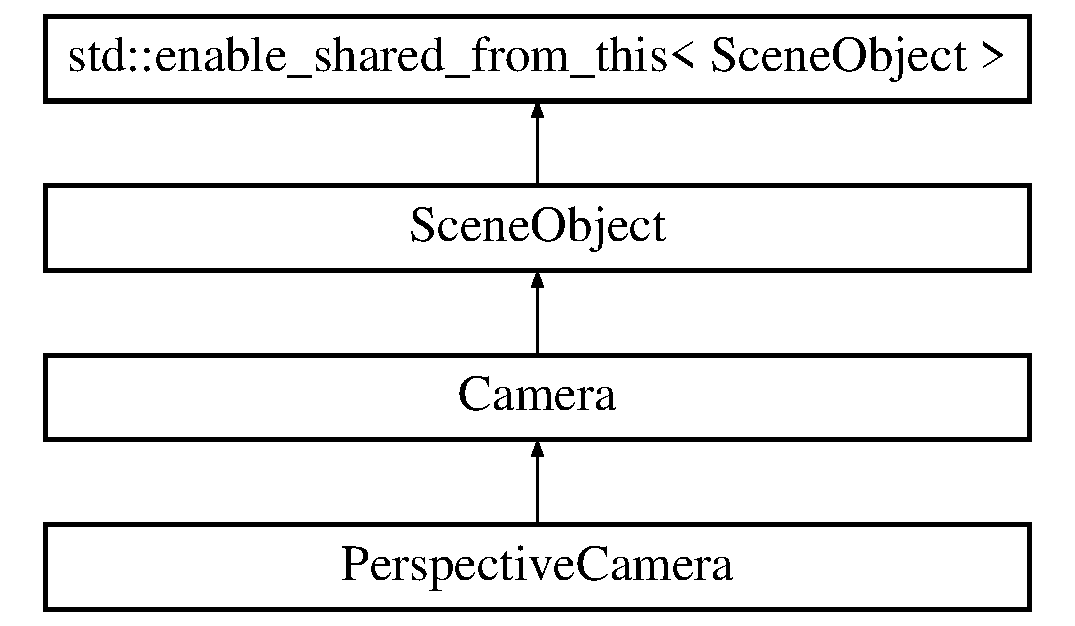
\includegraphics[height=4.000000cm]{class_perspective_camera}
\end{center}
\end{figure}
\subsection*{Public Member Functions}
\begin{DoxyCompactItemize}
\item
\hyperlink{class_perspective_camera_adb5624bfee18c9390df3ba0612431124}{Perspective\+Camera} (float in\+Fov, float in\+AR)
\item
virtual glm\+::mat4 \hyperlink{class_perspective_camera_ab467388c7d3e4c2ef9b498c16f291545}{Get\+Projection\+Matrix} () const
\begin{DoxyCompactList}\small\item\em Creates the projection matrix. \end{DoxyCompactList}\item
virtual float \hyperlink{class_perspective_camera_a04749345688970ec94fb26817bab10be}{Get\+F\+OV} () const
\begin{DoxyCompactList}\small\item\em Retrieve the vertical F\+OV. \end{DoxyCompactList}\item
virtual void \hyperlink{class_perspective_camera_a03f2ce1c0940599712b12a07719b5122}{Set\+F\+OV} (float in)
\begin{DoxyCompactList}\small\item\em Set the vertical F\+OV. \end{DoxyCompactList}\item
virtual float \hyperlink{class_perspective_camera_a87fb95ff5289f9bb8658c33ed710ec17}{Get\+Aspect\+Ratio} () const
\item
virtual void \hyperlink{class_perspective_camera_a2f8753cd16d119ed00d050b4dbac2510}{Set\+Aspect\+Ratio} (float in)
\item
virtual float \hyperlink{class_perspective_camera_ad9bd7e6bccb38c178dbd90d8d0a5778b}{Get\+Z\+Near} () const
\item
virtual void \hyperlink{class_perspective_camera_ab9bab141c767e0b604b213f482f72c8a}{Set\+Z\+Near} (float in)
\item
virtual float \hyperlink{class_perspective_camera_ae2e2bbd9e4bb5126c6f1de1606cd9c3e}{Get\+Z\+Far} () const
\item
virtual void \hyperlink{class_perspective_camera_a4374ca73880370dad1b93eaf489c9bb4}{Set\+Z\+Far} (float in)
\end{DoxyCompactItemize}
\subsection*{Protected Member Functions}
\begin{DoxyCompactItemize}
\item
virtual void \hyperlink{class_perspective_camera_a2f17fb07425e2146d5692805753fa368}{Update\+Transformation\+Matrix} ()
\begin{DoxyCompactList}\small\item\em Override the \hyperlink{class_scene_object_a20e31da3f9d2765de50cdb2d637ae6c9}{Scene\+Object\+::\+Update\+Transformation\+Matrix()} to do nothing. \end{DoxyCompactList}\end{DoxyCompactItemize}
\subsection*{Private Attributes}
\begin{DoxyCompactItemize}
\item
float \hyperlink{class_perspective_camera_ad693187f75ab5bfc597066364483325c}{fov}
\item
float \hyperlink{class_perspective_camera_ad96660d3109e54fa282955bf66a255eb}{aspect\+Ratio}
\item
float \hyperlink{class_perspective_camera_a11c1dcd1bdeb4bf8294d6272fb4d2695}{z\+Near}
\item
float \hyperlink{class_perspective_camera_af88e6161cd3c818d49e6421f52474a2b}{z\+Far}
\end{DoxyCompactItemize}
\subsection*{Additional Inherited Members}


\subsection{Detailed Description}
\hyperlink{class_camera}{Camera} that performs perspective projection.

\begin{DoxyWarning}{Warning}
The F\+OV in this class is the V\+E\+R\+T\+I\+C\+AL field of view. If you are familiar with video games, the F\+OV is usually presented to you as the H\+O\+R\+I\+Z\+O\+N\+T\+AL field of view which is usually wider than the vertical field of view! Be careful! Setting your vertical field of view to something like 120 degrees is insane!
\end{DoxyWarning}
We will not be covering the math behind perspective projection in this class, but you can read about it on the \href{https://en.wikipedia.org/wiki/3D_projection#Perspective_projection}{\tt Wikipedia page} or \href{http://ogldev.atspace.co.uk/www/tutorial12/tutorial12.html}{\tt this tutorial} if you are interested. The variables and functions in this class are just parameters to calculate the perspective projection matrix.

\subsection{Constructor \& Destructor Documentation}
\hypertarget{class_perspective_camera_adb5624bfee18c9390df3ba0612431124}{}\label{class_perspective_camera_adb5624bfee18c9390df3ba0612431124}
\index{Perspective\+Camera@{Perspective\+Camera}!Perspective\+Camera@{Perspective\+Camera}}
\index{Perspective\+Camera@{Perspective\+Camera}!Perspective\+Camera@{Perspective\+Camera}}
\subsubsection{\texorpdfstring{Perspective\+Camera()}{PerspectiveCamera()}}
{\footnotesize\ttfamily Perspective\+Camera\+::\+Perspective\+Camera (\begin{DoxyParamCaption}\item[{float}]{in\+Fov,  }\item[{float}]{in\+AR }\end{DoxyParamCaption})}



\subsection{Member Function Documentation}
\hypertarget{class_perspective_camera_a87fb95ff5289f9bb8658c33ed710ec17}{}\label{class_perspective_camera_a87fb95ff5289f9bb8658c33ed710ec17}
\index{Perspective\+Camera@{Perspective\+Camera}!Get\+Aspect\+Ratio@{Get\+Aspect\+Ratio}}
\index{Get\+Aspect\+Ratio@{Get\+Aspect\+Ratio}!Perspective\+Camera@{Perspective\+Camera}}
\subsubsection{\texorpdfstring{Get\+Aspect\+Ratio()}{GetAspectRatio()}}
{\footnotesize\ttfamily virtual float Perspective\+Camera\+::\+Get\+Aspect\+Ratio (\begin{DoxyParamCaption}{ }\end{DoxyParamCaption}) const\hspace{0.3cm}{\ttfamily [inline]}, {\ttfamily [virtual]}}

\hypertarget{class_perspective_camera_a04749345688970ec94fb26817bab10be}{}\label{class_perspective_camera_a04749345688970ec94fb26817bab10be}
\index{Perspective\+Camera@{Perspective\+Camera}!Get\+F\+OV@{Get\+F\+OV}}
\index{Get\+F\+OV@{Get\+F\+OV}!Perspective\+Camera@{Perspective\+Camera}}
\subsubsection{\texorpdfstring{Get\+F\+O\+V()}{GetFOV()}}
{\footnotesize\ttfamily virtual float Perspective\+Camera\+::\+Get\+F\+OV (\begin{DoxyParamCaption}{ }\end{DoxyParamCaption}) const\hspace{0.3cm}{\ttfamily [inline]}, {\ttfamily [virtual]}}



Retrieve the vertical F\+OV.

\begin{DoxyReturn}{Returns}
The vertical F\+OV in degrees.
\end{DoxyReturn}
\hypertarget{class_perspective_camera_ab467388c7d3e4c2ef9b498c16f291545}{}\label{class_perspective_camera_ab467388c7d3e4c2ef9b498c16f291545}
\index{Perspective\+Camera@{Perspective\+Camera}!Get\+Projection\+Matrix@{Get\+Projection\+Matrix}}
\index{Get\+Projection\+Matrix@{Get\+Projection\+Matrix}!Perspective\+Camera@{Perspective\+Camera}}
\subsubsection{\texorpdfstring{Get\+Projection\+Matrix()}{GetProjectionMatrix()}}
{\footnotesize\ttfamily glm\+::mat4 Perspective\+Camera\+::\+Get\+Projection\+Matrix (\begin{DoxyParamCaption}{ }\end{DoxyParamCaption}) const\hspace{0.3cm}{\ttfamily [virtual]}}



Creates the projection matrix.

\begin{DoxyReturn}{Returns}
The identity matrix.
\end{DoxyReturn}
This matrix will be the \char`\"{}\+P\char`\"{} in the M\+VP matrices.

Reimplemented from \hyperlink{class_camera_af6f4415189deaff158ba86f0b3527a30}{Camera}.

\hypertarget{class_perspective_camera_ae2e2bbd9e4bb5126c6f1de1606cd9c3e}{}\label{class_perspective_camera_ae2e2bbd9e4bb5126c6f1de1606cd9c3e}
\index{Perspective\+Camera@{Perspective\+Camera}!Get\+Z\+Far@{Get\+Z\+Far}}
\index{Get\+Z\+Far@{Get\+Z\+Far}!Perspective\+Camera@{Perspective\+Camera}}
\subsubsection{\texorpdfstring{Get\+Z\+Far()}{GetZFar()}}
{\footnotesize\ttfamily virtual float Perspective\+Camera\+::\+Get\+Z\+Far (\begin{DoxyParamCaption}{ }\end{DoxyParamCaption}) const\hspace{0.3cm}{\ttfamily [inline]}, {\ttfamily [virtual]}}

\hypertarget{class_perspective_camera_ad9bd7e6bccb38c178dbd90d8d0a5778b}{}\label{class_perspective_camera_ad9bd7e6bccb38c178dbd90d8d0a5778b}
\index{Perspective\+Camera@{Perspective\+Camera}!Get\+Z\+Near@{Get\+Z\+Near}}
\index{Get\+Z\+Near@{Get\+Z\+Near}!Perspective\+Camera@{Perspective\+Camera}}
\subsubsection{\texorpdfstring{Get\+Z\+Near()}{GetZNear()}}
{\footnotesize\ttfamily virtual float Perspective\+Camera\+::\+Get\+Z\+Near (\begin{DoxyParamCaption}{ }\end{DoxyParamCaption}) const\hspace{0.3cm}{\ttfamily [inline]}, {\ttfamily [virtual]}}

\hypertarget{class_perspective_camera_a2f8753cd16d119ed00d050b4dbac2510}{}\label{class_perspective_camera_a2f8753cd16d119ed00d050b4dbac2510}
\index{Perspective\+Camera@{Perspective\+Camera}!Set\+Aspect\+Ratio@{Set\+Aspect\+Ratio}}
\index{Set\+Aspect\+Ratio@{Set\+Aspect\+Ratio}!Perspective\+Camera@{Perspective\+Camera}}
\subsubsection{\texorpdfstring{Set\+Aspect\+Ratio()}{SetAspectRatio()}}
{\footnotesize\ttfamily virtual void Perspective\+Camera\+::\+Set\+Aspect\+Ratio (\begin{DoxyParamCaption}\item[{float}]{in }\end{DoxyParamCaption})\hspace{0.3cm}{\ttfamily [inline]}, {\ttfamily [virtual]}}

\hypertarget{class_perspective_camera_a03f2ce1c0940599712b12a07719b5122}{}\label{class_perspective_camera_a03f2ce1c0940599712b12a07719b5122}
\index{Perspective\+Camera@{Perspective\+Camera}!Set\+F\+OV@{Set\+F\+OV}}
\index{Set\+F\+OV@{Set\+F\+OV}!Perspective\+Camera@{Perspective\+Camera}}
\subsubsection{\texorpdfstring{Set\+F\+O\+V()}{SetFOV()}}
{\footnotesize\ttfamily virtual void Perspective\+Camera\+::\+Set\+F\+OV (\begin{DoxyParamCaption}\item[{float}]{in }\end{DoxyParamCaption})\hspace{0.3cm}{\ttfamily [inline]}, {\ttfamily [virtual]}}



Set the vertical F\+OV.


\begin{DoxyParams}{Parameters}
{\em in} & The vertical F\+OV in degrees. \\
\hline
\end{DoxyParams}
\hypertarget{class_perspective_camera_a4374ca73880370dad1b93eaf489c9bb4}{}\label{class_perspective_camera_a4374ca73880370dad1b93eaf489c9bb4}
\index{Perspective\+Camera@{Perspective\+Camera}!Set\+Z\+Far@{Set\+Z\+Far}}
\index{Set\+Z\+Far@{Set\+Z\+Far}!Perspective\+Camera@{Perspective\+Camera}}
\subsubsection{\texorpdfstring{Set\+Z\+Far()}{SetZFar()}}
{\footnotesize\ttfamily virtual void Perspective\+Camera\+::\+Set\+Z\+Far (\begin{DoxyParamCaption}\item[{float}]{in }\end{DoxyParamCaption})\hspace{0.3cm}{\ttfamily [inline]}, {\ttfamily [virtual]}}

\hypertarget{class_perspective_camera_ab9bab141c767e0b604b213f482f72c8a}{}\label{class_perspective_camera_ab9bab141c767e0b604b213f482f72c8a}
\index{Perspective\+Camera@{Perspective\+Camera}!Set\+Z\+Near@{Set\+Z\+Near}}
\index{Set\+Z\+Near@{Set\+Z\+Near}!Perspective\+Camera@{Perspective\+Camera}}
\subsubsection{\texorpdfstring{Set\+Z\+Near()}{SetZNear()}}
{\footnotesize\ttfamily virtual void Perspective\+Camera\+::\+Set\+Z\+Near (\begin{DoxyParamCaption}\item[{float}]{in }\end{DoxyParamCaption})\hspace{0.3cm}{\ttfamily [inline]}, {\ttfamily [virtual]}}

\hypertarget{class_perspective_camera_a2f17fb07425e2146d5692805753fa368}{}\label{class_perspective_camera_a2f17fb07425e2146d5692805753fa368}
\index{Perspective\+Camera@{Perspective\+Camera}!Update\+Transformation\+Matrix@{Update\+Transformation\+Matrix}}
\index{Update\+Transformation\+Matrix@{Update\+Transformation\+Matrix}!Perspective\+Camera@{Perspective\+Camera}}
\subsubsection{\texorpdfstring{Update\+Transformation\+Matrix()}{UpdateTransformationMatrix()}}
{\footnotesize\ttfamily void Perspective\+Camera\+::\+Update\+Transformation\+Matrix (\begin{DoxyParamCaption}{ }\end{DoxyParamCaption})\hspace{0.3cm}{\ttfamily [protected]}, {\ttfamily [virtual]}}



Override the \hyperlink{class_scene_object_a20e31da3f9d2765de50cdb2d637ae6c9}{Scene\+Object\+::\+Update\+Transformation\+Matrix()} to do nothing.

This will guarantee that the transformation matrix will always be an identity matrix regardless of whether you move/rotate/scale the camera.

Reimplemented from \hyperlink{class_camera_aea640c892a3807671d8ca49616d96eda}{Camera}.



\subsection{Member Data Documentation}
\hypertarget{class_perspective_camera_ad96660d3109e54fa282955bf66a255eb}{}\label{class_perspective_camera_ad96660d3109e54fa282955bf66a255eb}
\index{Perspective\+Camera@{Perspective\+Camera}!aspect\+Ratio@{aspect\+Ratio}}
\index{aspect\+Ratio@{aspect\+Ratio}!Perspective\+Camera@{Perspective\+Camera}}
\subsubsection{\texorpdfstring{aspect\+Ratio}{aspectRatio}}
{\footnotesize\ttfamily float Perspective\+Camera\+::aspect\+Ratio\hspace{0.3cm}{\ttfamily [private]}}

\hypertarget{class_perspective_camera_ad693187f75ab5bfc597066364483325c}{}\label{class_perspective_camera_ad693187f75ab5bfc597066364483325c}
\index{Perspective\+Camera@{Perspective\+Camera}!fov@{fov}}
\index{fov@{fov}!Perspective\+Camera@{Perspective\+Camera}}
\subsubsection{\texorpdfstring{fov}{fov}}
{\footnotesize\ttfamily float Perspective\+Camera\+::fov\hspace{0.3cm}{\ttfamily [private]}}

\hypertarget{class_perspective_camera_af88e6161cd3c818d49e6421f52474a2b}{}\label{class_perspective_camera_af88e6161cd3c818d49e6421f52474a2b}
\index{Perspective\+Camera@{Perspective\+Camera}!z\+Far@{z\+Far}}
\index{z\+Far@{z\+Far}!Perspective\+Camera@{Perspective\+Camera}}
\subsubsection{\texorpdfstring{z\+Far}{zFar}}
{\footnotesize\ttfamily float Perspective\+Camera\+::z\+Far\hspace{0.3cm}{\ttfamily [private]}}

\hypertarget{class_perspective_camera_a11c1dcd1bdeb4bf8294d6272fb4d2695}{}\label{class_perspective_camera_a11c1dcd1bdeb4bf8294d6272fb4d2695}
\index{Perspective\+Camera@{Perspective\+Camera}!z\+Near@{z\+Near}}
\index{z\+Near@{z\+Near}!Perspective\+Camera@{Perspective\+Camera}}
\subsubsection{\texorpdfstring{z\+Near}{zNear}}
{\footnotesize\ttfamily float Perspective\+Camera\+::z\+Near\hspace{0.3cm}{\ttfamily [private]}}



The documentation for this class was generated from the following files\+:\begin{DoxyCompactItemize}
\item
/data/MO814A-MC937A/MO814A-MC937Aopengl-\/instructor/source/common/\+Scene/\+Camera/\hyperlink{_perspective_camera_8h}{Perspective\+Camera.\+h}\item
/data/MO814A-MC937A/MO814A-MC937Aopengl-\/instructor/source/common/\+Scene/\+Camera/\hyperlink{_perspective_camera_8cpp}{Perspective\+Camera.\+cpp}\end{DoxyCompactItemize}

\hypertarget{class_renderer}{}\section{Renderer Class Reference}
\label{class_renderer}\index{Renderer@{Renderer}}


A generic rendering interface.




{\ttfamily \#include $<$Renderer.\+h$>$}

Inheritance diagram for Renderer\+:\begin{figure}[H]
\begin{center}
\leavevmode
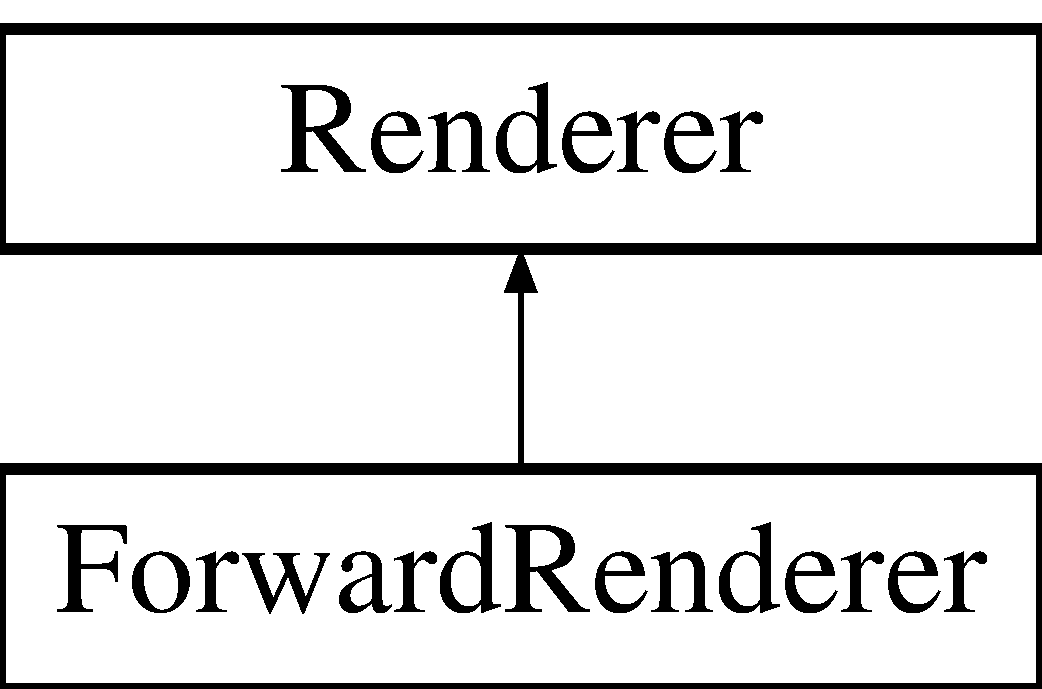
\includegraphics[height=2.000000cm]{class_renderer}
\end{center}
\end{figure}
\subsection*{Public Member Functions}
\begin{DoxyCompactItemize}
\item 
\hyperlink{class_renderer_adc8ce31cd649bdf220ca8355809b1d06}{Renderer} (std\+::shared\+\_\+ptr$<$ class \hyperlink{class_scene}{Scene} $>$ input\+Scene, std\+::shared\+\_\+ptr$<$ class \hyperlink{class_camera}{Camera} $>$ input\+Camera)
\begin{DoxyCompactList}\small\item\em The \hyperlink{class_renderer}{Renderer} constructor takes in a scene to be rendered and the camera from which to render the scene. \end{DoxyCompactList}\item
virtual \hyperlink{class_renderer_afeee408862d5bd6255a6882d47e6d5cd}{$\sim$\+Renderer} ()
\begin{DoxyCompactList}\small\item\em A virtual destructor to allow for safe inheritance. \end{DoxyCompactList}\item
virtual void \hyperlink{class_renderer_a7cb221f355f181d84d66e8c09f50f04a}{Initialize} ()=0
\begin{DoxyCompactList}\small\item\em Prepares the renderer for usage. \end{DoxyCompactList}\item
virtual void \hyperlink{class_renderer_a38623da22aa718cfa41e2514ebd269f5}{Render} ()=0
\begin{DoxyCompactList}\small\item\em This function should be used to render everything onto the screen. \end{DoxyCompactList}\end{DoxyCompactItemize}
\subsection*{Protected Attributes}
\begin{DoxyCompactItemize}
\item
std\+::shared\+\_\+ptr$<$ class \hyperlink{class_scene}{Scene} $>$ \hyperlink{class_renderer_a65178695d48824d3afd6fe40fd4915b6}{scene}
\begin{DoxyCompactList}\small\item\em Shared pointer to the scene. Should not be a null pointer when you go to render. \end{DoxyCompactList}\item
std\+::shared\+\_\+ptr$<$ class \hyperlink{class_camera}{Camera} $>$ \hyperlink{class_renderer_a7a08c6489c1ffe8e346b9f205b4014ca}{camera}
\begin{DoxyCompactList}\small\item\em Shared pointer to the camera. Should not be a null pointer when you go to render. \end{DoxyCompactList}\end{DoxyCompactItemize}


\subsection{Detailed Description}
A generic rendering interface.

The renderer will be used by the \hyperlink{class_media_layer}{Media\+Layer} and will be told to \hyperlink{class_renderer_a38623da22aa718cfa41e2514ebd269f5}{Render()} every frame. It is the renderer\textquotesingle{}s responsibility to make sure everything in the scene gets rendered properly with the right shader using all the lights.

\subsection{Constructor \& Destructor Documentation}
\hypertarget{class_renderer_adc8ce31cd649bdf220ca8355809b1d06}{}\label{class_renderer_adc8ce31cd649bdf220ca8355809b1d06}
\index{Renderer@{Renderer}!Renderer@{Renderer}}
\index{Renderer@{Renderer}!Renderer@{Renderer}}
\subsubsection{\texorpdfstring{Renderer()}{Renderer()}}
{\footnotesize\ttfamily Renderer\+::\+Renderer (\begin{DoxyParamCaption}\item[{std\+::shared\+\_\+ptr$<$ class \hyperlink{class_scene}{Scene} $>$}]{input\+Scene,  }\item[{std\+::shared\+\_\+ptr$<$ class \hyperlink{class_camera}{Camera} $>$}]{input\+Camera }\end{DoxyParamCaption})}



The \hyperlink{class_renderer}{Renderer} constructor takes in a scene to be rendered and the camera from which to render the scene.


\begin{DoxyParams}{Parameters}
{\em input\+Scene} & A shared pointer to the scene. This can be a null pointer but you would need to introduce functions to set it later. \\
\hline
{\em input\+Camera} & A shared pointer to the camera. This can be a null pointer but you would need to introduce functions to set it later. \\
\hline
\end{DoxyParams}
\hypertarget{class_renderer_afeee408862d5bd6255a6882d47e6d5cd}{}\label{class_renderer_afeee408862d5bd6255a6882d47e6d5cd}
\index{Renderer@{Renderer}!````~Renderer@{$\sim$\+Renderer}}
\index{````~Renderer@{$\sim$\+Renderer}!Renderer@{Renderer}}
\subsubsection{\texorpdfstring{$\sim$\+Renderer()}{~Renderer()}}
{\footnotesize\ttfamily Renderer\+::$\sim$\+Renderer (\begin{DoxyParamCaption}{ }\end{DoxyParamCaption})\hspace{0.3cm}{\ttfamily [virtual]}}



A virtual destructor to allow for safe inheritance.



\subsection{Member Function Documentation}
\hypertarget{class_renderer_a7cb221f355f181d84d66e8c09f50f04a}{}\label{class_renderer_a7cb221f355f181d84d66e8c09f50f04a}
\index{Renderer@{Renderer}!Initialize@{Initialize}}
\index{Initialize@{Initialize}!Renderer@{Renderer}}
\subsubsection{\texorpdfstring{Initialize()}{Initialize()}}
{\footnotesize\ttfamily virtual void Renderer\+::\+Initialize (\begin{DoxyParamCaption}{ }\end{DoxyParamCaption})\hspace{0.3cm}{\ttfamily [pure virtual]}}



Prepares the renderer for usage.

Called in the \hyperlink{class_media_layer}{Media\+Layer} constructor.

Implemented in \hyperlink{class_forward_renderer_a5cbca647822780d6cfbd39552d73ee06}{Forward\+Renderer}.

\hypertarget{class_renderer_a38623da22aa718cfa41e2514ebd269f5}{}\label{class_renderer_a38623da22aa718cfa41e2514ebd269f5}
\index{Renderer@{Renderer}!Render@{Render}}
\index{Render@{Render}!Renderer@{Renderer}}
\subsubsection{\texorpdfstring{Render()}{Render()}}
{\footnotesize\ttfamily virtual void Renderer\+::\+Render (\begin{DoxyParamCaption}{ }\end{DoxyParamCaption})\hspace{0.3cm}{\ttfamily [pure virtual]}}



This function should be used to render everything onto the screen.



Implemented in \hyperlink{class_forward_renderer_a1a5deafa5deaf1e0abaab0e2074928c1}{Forward\+Renderer}.



\subsection{Member Data Documentation}
\hypertarget{class_renderer_a7a08c6489c1ffe8e346b9f205b4014ca}{}\label{class_renderer_a7a08c6489c1ffe8e346b9f205b4014ca}
\index{Renderer@{Renderer}!camera@{camera}}
\index{camera@{camera}!Renderer@{Renderer}}
\subsubsection{\texorpdfstring{camera}{camera}}
{\footnotesize\ttfamily std\+::shared\+\_\+ptr$<$class \hyperlink{class_camera}{Camera}$>$ Renderer\+::camera\hspace{0.3cm}{\ttfamily [protected]}}



Shared pointer to the camera. Should not be a null pointer when you go to render.

\hypertarget{class_renderer_a65178695d48824d3afd6fe40fd4915b6}{}\label{class_renderer_a65178695d48824d3afd6fe40fd4915b6}
\index{Renderer@{Renderer}!scene@{scene}}
\index{scene@{scene}!Renderer@{Renderer}}
\subsubsection{\texorpdfstring{scene}{scene}}
{\footnotesize\ttfamily std\+::shared\+\_\+ptr$<$class \hyperlink{class_scene}{Scene}$>$ Renderer\+::scene\hspace{0.3cm}{\ttfamily [protected]}}



Shared pointer to the scene. Should not be a null pointer when you go to render.



The documentation for this class was generated from the following files\+:\begin{DoxyCompactItemize}
\item
/data/MO814A-MC937A/MO814A-MC937Aopengl-\/instructor/source/common/\+Rendering/\hyperlink{_renderer_8h}{Renderer.\+h}\item
/data/MO814A-MC937A/MO814A-MC937Aopengl-\/instructor/source/common/\+Rendering/\hyperlink{_renderer_8cpp}{Renderer.\+cpp}\end{DoxyCompactItemize}

\hypertarget{class_rendering_object}{}\section{Rendering\+Object Class Reference}
\label{class_rendering_object}\index{Rendering\+Object@{Rendering\+Object}}


Stores the vertex data for a mesh.




{\ttfamily \#include $<$Rendering\+Object.\+h$>$}

\subsection*{Public Types}
\begin{DoxyCompactItemize}
\item
enum \hyperlink{class_rendering_object_ab772f569ef63a1db07db29a744b519ee}{Vertex\+Attribute\+Positions} \{ \newline
\hyperlink{class_rendering_object_ab772f569ef63a1db07db29a744b519eea52f5e0bc3859bc5f5e25130b6c7e8881}{Vertex\+Attribute\+Positions\+::\+Position} = 0,
\hyperlink{class_rendering_object_ab772f569ef63a1db07db29a744b519eea4ab971a51f0335cbf8d9c2c65d379e99}{Vertex\+Attribute\+Positions\+::\+Normals},
\hyperlink{class_rendering_object_ab772f569ef63a1db07db29a744b519eeadeaa2adbeb26802ae61609c3f3642d82}{Vertex\+Attribute\+Positions\+::\+UV},
\hyperlink{class_rendering_object_ab772f569ef63a1db07db29a744b519eea5d50889672f6f860d14f502de3de1957}{Vertex\+Attribute\+Positions\+::\+Colors},
\newline
\hyperlink{class_rendering_object_ab772f569ef63a1db07db29a744b519eea541671cb1be09d76a84ba1a873ec3fc8}{Vertex\+Attribute\+Positions\+::\+Tangent},
\hyperlink{class_rendering_object_ab772f569ef63a1db07db29a744b519eeae3e73a4b6e7cfd12008a35f6a051b319}{Vertex\+Attribute\+Positions\+::\+Bitangent}
 \}\begin{DoxyCompactList}\small\item\em This enum has its values corresponding to the layout location qualifer on the vertex attribute array. \end{DoxyCompactList}
\item
using \hyperlink{class_rendering_object_a1223b9cf03f2029b9c43d71042c2a18e}{Position\+Array} = std\+::vector$<$ glm\+::vec4 $>$
\item
using \hyperlink{class_rendering_object_a9931c88bca3384065c6691dfe1e60af1}{Index\+Array} = std\+::vector$<$ unsigned int $>$
\item
using \hyperlink{class_rendering_object_a327c4d892de8d6138fb59afa6d078257}{Normal\+Array} = std\+::vector$<$ glm\+::vec3 $>$
\item
using \hyperlink{class_rendering_object_a504ecd45ebe36dfa5b78c46d64d9904a}{U\+V\+Array} = std\+::vector$<$ glm\+::vec2 $>$
\item
using \hyperlink{class_rendering_object_a8a12e1f9be788d99af6c089e1c600022}{Color\+Array} = std\+::vector$<$ glm\+::vec4 $>$
\item
using \hyperlink{class_rendering_object_a45b53e911c2f0131aa10e89869d38944}{Tangent\+Array} = std\+::vector$<$ glm\+::vec3 $>$
\item
using \hyperlink{class_rendering_object_a6c6bf305a5f0f9ce1006f374c753c856}{Bitangent\+Array} = std\+::vector$<$ glm\+::vec3 $>$
\end{DoxyCompactItemize}
\subsection*{Public Member Functions}
\begin{DoxyCompactItemize}
\item
\hyperlink{class_rendering_object_ab5e3376ea0eb6290cdc55750a420b9d1}{Rendering\+Object} (std\+::shared\+\_\+ptr$<$ class \hyperlink{class_shader_program}{Shader\+Program} $>$ input\+Shader, std\+::unique\+\_\+ptr$<$ \hyperlink{class_rendering_object_a1223b9cf03f2029b9c43d71042c2a18e}{Position\+Array} $>$ input\+Positions, std\+::unique\+\_\+ptr$<$ \hyperlink{class_rendering_object_a9931c88bca3384065c6691dfe1e60af1}{Index\+Array} $>$ input\+Indices=nullptr, std\+::unique\+\_\+ptr$<$ \hyperlink{class_rendering_object_a327c4d892de8d6138fb59afa6d078257}{Normal\+Array} $>$ input\+Normals=nullptr, std\+::unique\+\_\+ptr$<$ \hyperlink{class_rendering_object_a504ecd45ebe36dfa5b78c46d64d9904a}{U\+V\+Array} $>$ input\+UV=nullptr, std\+::unique\+\_\+ptr$<$ \hyperlink{class_rendering_object_a8a12e1f9be788d99af6c089e1c600022}{Color\+Array} $>$ input\+Colors=nullptr, std\+::unique\+\_\+ptr$<$ \hyperlink{class_rendering_object_a45b53e911c2f0131aa10e89869d38944}{Tangent\+Array} $>$ input\+Tangents=nullptr, std\+::unique\+\_\+ptr$<$ \hyperlink{class_rendering_object_a6c6bf305a5f0f9ce1006f374c753c856}{Bitangent\+Array} $>$ input\+Bitangents=nullptr)
\begin{DoxyCompactList}\small\item\em Constructs a \hyperlink{class_rendering_object}{Rendering\+Object} from a shader and all the possible vertex attributes. \end{DoxyCompactList}\item
virtual \hyperlink{class_rendering_object_ae4e8e14104ee3a587d10c9f90ec82048}{$\sim$\+Rendering\+Object} ()
\begin{DoxyCompactList}\small\item\em Just another deconstructor. \end{DoxyCompactList}\item
virtual void \hyperlink{class_rendering_object_a22311d08bb7559f6b913afe314a5031e}{Set\+Shader} (std\+::shared\+\_\+ptr$<$ class \hyperlink{class_shader_program}{Shader\+Program} $>$ input\+Shader)
\begin{DoxyCompactList}\small\item\em Sets the shader to be used to render this object. \end{DoxyCompactList}\item
virtual void \hyperlink{class_rendering_object_a878582ad56859856506a6d4c4be393e9}{Begin\+Render} () const
\begin{DoxyCompactList}\small\item\em Prepares to the mesh object. \end{DoxyCompactList}\item
virtual void \hyperlink{class_rendering_object_aee6affd69495adc61bae0e71433d353a}{Render} () const
\begin{DoxyCompactList}\small\item\em Calls the appropriate draw function depending on whether or not an element buffer object is used. \end{DoxyCompactList}\item
virtual void \hyperlink{class_rendering_object_abc5f87208a9c918f3d281dd673cb5a24}{End\+Render} () const
\begin{DoxyCompactList}\small\item\em Unbinds the V\+AO and the E\+BO to cleanup the state. \end{DoxyCompactList}\item
void \hyperlink{class_rendering_object_aa627eb310f11d0e04dbbb3665f58bb4e}{Set\+Draw\+Mode} (G\+Lenum input\+Mode)
\begin{DoxyCompactList}\small\item\em Sets what kind of primitives Open\+GL should interpret the data as. \end{DoxyCompactList}\item
G\+Lint \hyperlink{class_rendering_object_abe3637190e30c5483e9505743c75bcdb}{Get\+Shader\+Program} () const
\begin{DoxyCompactList}\small\item\em Returns the Open\+GL identifier for the underlying shader program. \end{DoxyCompactList}\item
const class \hyperlink{class_shader_program}{Shader\+Program} $\ast$ \hyperlink{class_rendering_object_ab32a982b996ebaca66f4f8b9f4e548b2}{Get\+Shader\+Program\+Raw} () const
\begin{DoxyCompactList}\small\item\em Returns a raw pointer to the underlying shader program. \end{DoxyCompactList}\item
size\+\_\+t \hyperlink{class_rendering_object_af83dd72431c620145b06d2e1bf7a9f3e}{Get\+Total\+Vertices} () const
\begin{DoxyCompactList}\small\item\em Returns the total number of vertices. \end{DoxyCompactList}\item
virtual void \hyperlink{class_rendering_object_ada51886b7da1924a17d3a55e8fe90061}{Set\+Vertex\+Positions} (std\+::unique\+\_\+ptr$<$ \hyperlink{class_rendering_object_a1223b9cf03f2029b9c43d71042c2a18e}{Position\+Array} $>$ positions)
\begin{DoxyCompactList}\small\item\em Sets the vertex positions array. Also updates the data stored in the vertex buffer object. \end{DoxyCompactList}\item
virtual void \hyperlink{class_rendering_object_a61ea597df0c456834eac8eb4087fb573}{Set\+Vertex\+Indices} (std\+::unique\+\_\+ptr$<$ \hyperlink{class_rendering_object_a9931c88bca3384065c6691dfe1e60af1}{Index\+Array} $>$ indices)
\begin{DoxyCompactList}\small\item\em Sets the vertex indices array. Also updates the data stored in the element buffer object. \end{DoxyCompactList}\item
virtual void \hyperlink{class_rendering_object_a4cd085aed01fbc5e4fae7076e00919d3}{Set\+Vertex\+Normals} (std\+::unique\+\_\+ptr$<$ \hyperlink{class_rendering_object_a327c4d892de8d6138fb59afa6d078257}{Normal\+Array} $>$ normals)
\begin{DoxyCompactList}\small\item\em Sets the vertex normal array. Also updates the data stored in the vertex buffer object. \end{DoxyCompactList}\item
virtual void \hyperlink{class_rendering_object_a2a2b3c6ec2d13e8d3a4b6ac4c05ae11b}{Set\+Vertex\+UV} (std\+::unique\+\_\+ptr$<$ \hyperlink{class_rendering_object_a504ecd45ebe36dfa5b78c46d64d9904a}{U\+V\+Array} $>$ uv)
\begin{DoxyCompactList}\small\item\em Sets the vertex UV array. Also updates the data stored in the vertex buffer object. \end{DoxyCompactList}\item
virtual void \hyperlink{class_rendering_object_aa1170c47ff02b2305a54c8aab3460201}{Set\+Vertex\+Colors} (std\+::unique\+\_\+ptr$<$ \hyperlink{class_rendering_object_a8a12e1f9be788d99af6c089e1c600022}{Color\+Array} $>$ colors)
\begin{DoxyCompactList}\small\item\em Sets the vertex color array. Also updates the data stored in the vertex buffer object. \end{DoxyCompactList}\item
virtual void \hyperlink{class_rendering_object_a041c99c6f0d570bb7c36b9d2168f0b0d}{Set\+Vertex\+Tangents} (std\+::unique\+\_\+ptr$<$ \hyperlink{class_rendering_object_a45b53e911c2f0131aa10e89869d38944}{Tangent\+Array} $>$ input)
\item
virtual void \hyperlink{class_rendering_object_a095317dd60a7558c22409e2fabcb252e}{Set\+Vertex\+Bitangents} (std\+::unique\+\_\+ptr$<$ \hyperlink{class_rendering_object_a6c6bf305a5f0f9ce1006f374c753c856}{Bitangent\+Array} $>$ input)
\item
virtual void \hyperlink{class_rendering_object_adec25796def807fd09a5fc4f1fbd0c41}{Compute\+Tangent\+Space} ()
\item
virtual void \hyperlink{class_rendering_object_a761ad8574fc4424e12487512bb30067c}{Reverse\+Normals} ()
\item
virtual void \hyperlink{class_rendering_object_a2f175770ceadac2fea979f191974665b}{Reverse\+Vertex\+Order} ()
\end{DoxyCompactItemize}
\subsection*{Protected Member Functions}
\begin{DoxyCompactItemize}
\item
virtual void \hyperlink{class_rendering_object_a77c78d1b42ea2ebfdbf994b6b91ce805}{Initialize\+Open\+GL} ()
\begin{DoxyCompactList}\small\item\em Prepares the rendering object for use by Open\+GL. \end{DoxyCompactList}\item
virtual void \hyperlink{class_rendering_object_a7a097727acf37f9671ddd5e3a9873771}{Update\+Vertex\+Positions} ()
\item
virtual void \hyperlink{class_rendering_object_afb49054121b1b552bce58625db91b851}{Update\+Vertex\+Indices} ()
\item
virtual void \hyperlink{class_rendering_object_ae4b537e1c9b1c5c50cb7b0db83e6f190}{Update\+Vertex\+Normals} ()
\item
virtual void \hyperlink{class_rendering_object_ac00889f2afaa605b09164649ef68a1b6}{Update\+Vertex\+UV} ()
\item
virtual void \hyperlink{class_rendering_object_aca18dbb9252f27cef09df307dbcf02a9}{Update\+Vertex\+Colors} ()
\item
virtual void \hyperlink{class_rendering_object_a5b480a9b97cadfa07669902764139272}{Update\+Vertex\+Tangents} ()
\item
virtual void \hyperlink{class_rendering_object_a594a50e9475057aaf21a0b05b33a5b16}{Update\+Vertex\+Bitangents} ()
\item
virtual void \hyperlink{class_rendering_object_af9c1a07398071cdd0cca3ad36095fc85}{Cleanup\+Vertex\+Positions} ()
\item
virtual void \hyperlink{class_rendering_object_ac60c8a7f3d5678fd4aa8198f6c980e6e}{Cleanup\+Vertex\+Indices} ()
\item
virtual void \hyperlink{class_rendering_object_ad89bc24893f8fe32794f0686c2bb0da1}{Cleanup\+Vertex\+Normals} ()
\item
virtual void \hyperlink{class_rendering_object_a776f54b41f9e9f0e55fc1104919c3e7c}{Cleanup\+Vertex\+UV} ()
\item
virtual void \hyperlink{class_rendering_object_adce4a6d6406eb589b088bedd19127f32}{Cleanup\+Vertex\+Colors} ()
\item
virtual void \hyperlink{class_rendering_object_a0e6c8c9480f1c04202aa6d38a841f06f}{Cleanup\+Vertex\+Tangents} ()
\item
virtual void \hyperlink{class_rendering_object_ae60c4f13ea817ffcb722d34250664c41}{Cleanup\+Vertex\+Bitangents} ()
\end{DoxyCompactItemize}
\subsection*{Protected Attributes}
\begin{DoxyCompactItemize}
\item
std\+::shared\+\_\+ptr$<$ class \hyperlink{class_shader_program}{Shader\+Program} $>$ \hyperlink{class_rendering_object_ae50e545ce2008ffa802478cd4316e82e}{shader}
\begin{DoxyCompactList}\small\item\em The shader program used to render the object. \end{DoxyCompactList}\item
G\+Luint \hyperlink{class_rendering_object_a473f623b39157288bef992e76ddc45a9}{vertex\+Position\+Buffer}
\begin{DoxyCompactList}\small\item\em The buffer ID for the vertex position V\+BO as generated by \href{https://www.opengl.org/sdk/docs/man/html/glGenBuffers.xhtml}{\tt gl\+Gen\+Buffers}. \end{DoxyCompactList}\item
std\+::unique\+\_\+ptr$<$ \hyperlink{class_rendering_object_a1223b9cf03f2029b9c43d71042c2a18e}{Position\+Array} $>$ \hyperlink{class_rendering_object_a14721712672d0421ed72a394e3131da0}{vertex\+Positions}
\begin{DoxyCompactList}\small\item\em The position of every vertex. \end{DoxyCompactList}\item
G\+Luint \hyperlink{class_rendering_object_a6740a0a0e6bd4d841c9c211f2a31cca3}{vertex\+Index\+Buffer}
\begin{DoxyCompactList}\small\item\em The buffer ID for the vertex index E\+BO as generated by \href{https://www.opengl.org/sdk/docs/man/html/glGenBuffers.xhtml}{\tt gl\+Gen\+Buffers}. \end{DoxyCompactList}\item
std\+::unique\+\_\+ptr$<$ \hyperlink{class_rendering_object_a9931c88bca3384065c6691dfe1e60af1}{Index\+Array} $>$ \hyperlink{class_rendering_object_a7b84487d3c34c1ca36b2ac6060b0f802}{vertex\+Indices}
\begin{DoxyCompactList}\small\item\em The indices into the vertex array. This allows us to reuse vertices for multiple faces. \end{DoxyCompactList}\item
G\+Luint \hyperlink{class_rendering_object_a91649e3a653f2266cd00c718f10849f9}{vertex\+Normal\+Buffer}
\begin{DoxyCompactList}\small\item\em The buffer ID for the vertex normal V\+BO as generated by \href{https://www.opengl.org/sdk/docs/man/html/glGenBuffers.xhtml}{\tt gl\+Gen\+Buffers}. \end{DoxyCompactList}\item
std\+::unique\+\_\+ptr$<$ \hyperlink{class_rendering_object_a327c4d892de8d6138fb59afa6d078257}{Normal\+Array} $>$ \hyperlink{class_rendering_object_ac28d301f97d29ab603f65f8e823063b4}{vertex\+Normals}
\begin{DoxyCompactList}\small\item\em The normal of every vertex. \end{DoxyCompactList}\item
G\+Luint \hyperlink{class_rendering_object_a0eac563be6e35a3cc4409d43a2abaa04}{vertex\+Tangent\+Buffer}
\item
std\+::unique\+\_\+ptr$<$ \hyperlink{class_rendering_object_a45b53e911c2f0131aa10e89869d38944}{Tangent\+Array} $>$ \hyperlink{class_rendering_object_a7bca44786929dd3aca3d6ca1acc7597f}{vertex\+Tangents}
\item
G\+Luint \hyperlink{class_rendering_object_a0c2f16211e989dd4d9d2ebbf7c027fb6}{vertex\+Bitangent\+Buffer}
\item
std\+::unique\+\_\+ptr$<$ \hyperlink{class_rendering_object_a6c6bf305a5f0f9ce1006f374c753c856}{Bitangent\+Array} $>$ \hyperlink{class_rendering_object_a3d0ab70c5a87e4cd7fff87f3ee927678}{vertex\+Bitangents}
\item
G\+Luint \hyperlink{class_rendering_object_ad583c70014e3f6ab0c9b62ea3c96ad25}{vertex\+U\+V\+Buffer}
\begin{DoxyCompactList}\small\item\em The buffer ID for the vertex UV V\+BO as generated by \href{https://www.opengl.org/sdk/docs/man/html/glGenBuffers.xhtml}{\tt gl\+Gen\+Buffers}. \end{DoxyCompactList}\item
std\+::unique\+\_\+ptr$<$ \hyperlink{class_rendering_object_a504ecd45ebe36dfa5b78c46d64d9904a}{U\+V\+Array} $>$ \hyperlink{class_rendering_object_afc405316bddec4ba1d5c228ecc0d9061}{vertex\+UV}
\begin{DoxyCompactList}\small\item\em The UV coordinate of every vertex. \end{DoxyCompactList}\item
G\+Luint \hyperlink{class_rendering_object_aeb014a4ef24e2fc4665a769241660cad}{vertex\+Color\+Buffer}
\begin{DoxyCompactList}\small\item\em The buffer ID for the vertex color V\+BO as generated by \href{https://www.opengl.org/sdk/docs/man/html/glGenBuffers.xhtml}{\tt gl\+Gen\+Buffers}. \end{DoxyCompactList}\item
std\+::unique\+\_\+ptr$<$ \hyperlink{class_rendering_object_a8a12e1f9be788d99af6c089e1c600022}{Color\+Array} $>$ \hyperlink{class_rendering_object_a65fc52e665791ce55e43106b603e917a}{vertex\+Colors}
\begin{DoxyCompactList}\small\item\em The color of every vertex. \end{DoxyCompactList}\item
G\+Luint \hyperlink{class_rendering_object_a96dd05670a977a949514a2c490c1c867}{vao}
\item
G\+Lenum \hyperlink{class_rendering_object_aa67856a72705b54a5667e91e270d00b3}{draw\+Mode}
\end{DoxyCompactItemize}
\subsection*{Static Protected Attributes}
\begin{DoxyCompactItemize}
\item
static glm\+::vec3 \hyperlink{class_rendering_object_af270a476ba12c23fefbb034e21930add}{D\+E\+F\+A\+U\+L\+T\+\_\+\+N\+O\+R\+M\+AL}
\begin{DoxyCompactList}\small\item\em The default value sent to the shader if \hyperlink{class_rendering_object_ac28d301f97d29ab603f65f8e823063b4}{Rendering\+Object\+::vertex\+Normals} is not set. \end{DoxyCompactList}\item
static glm\+::vec2 \hyperlink{class_rendering_object_a3dcb28a12f578630aea75cc59ea39588}{D\+E\+F\+A\+U\+L\+T\+\_\+\+UV}
\begin{DoxyCompactList}\small\item\em The default value sent to the shader if \hyperlink{class_rendering_object_afc405316bddec4ba1d5c228ecc0d9061}{Rendering\+Object\+::vertex\+UV} is not set. \end{DoxyCompactList}\item
static glm\+::vec4 \hyperlink{class_rendering_object_a3bf21996dc0ef604b2b81d95275c97f9}{D\+E\+F\+A\+U\+L\+T\+\_\+\+C\+O\+L\+OR}
\begin{DoxyCompactList}\small\item\em The default value sent to the shader if \hyperlink{class_rendering_object_a65fc52e665791ce55e43106b603e917a}{Rendering\+Object\+::vertex\+Colors} is not set. \end{DoxyCompactList}\end{DoxyCompactItemize}
\subsection*{Private Member Functions}
\begin{DoxyCompactItemize}
\item
virtual void \hyperlink{class_rendering_object_a053e68759fe406779c6b6cfa080602bf}{Compute\+Tangent\+Space\+Helper} (glm\+::ivec3 triangle\+Vertex\+Indices, bool use\+Stored\+Normals, std\+::vector$<$ int $>$ \&averager)
\end{DoxyCompactItemize}


\subsection{Detailed Description}
Stores the vertex data for a mesh.

This class allows us to easily reuse the same mesh data for multiple objects in the scene.

\subsection{Member Typedef Documentation}
\hypertarget{class_rendering_object_a6c6bf305a5f0f9ce1006f374c753c856}{}\label{class_rendering_object_a6c6bf305a5f0f9ce1006f374c753c856}
\index{Rendering\+Object@{Rendering\+Object}!Bitangent\+Array@{Bitangent\+Array}}
\index{Bitangent\+Array@{Bitangent\+Array}!Rendering\+Object@{Rendering\+Object}}
\subsubsection{\texorpdfstring{Bitangent\+Array}{BitangentArray}}
{\footnotesize\ttfamily using \hyperlink{class_rendering_object_a6c6bf305a5f0f9ce1006f374c753c856}{Rendering\+Object\+::\+Bitangent\+Array} =  std\+::vector$<$glm\+::vec3$>$}

\hypertarget{class_rendering_object_a8a12e1f9be788d99af6c089e1c600022}{}\label{class_rendering_object_a8a12e1f9be788d99af6c089e1c600022}
\index{Rendering\+Object@{Rendering\+Object}!Color\+Array@{Color\+Array}}
\index{Color\+Array@{Color\+Array}!Rendering\+Object@{Rendering\+Object}}
\subsubsection{\texorpdfstring{Color\+Array}{ColorArray}}
{\footnotesize\ttfamily using \hyperlink{class_rendering_object_a8a12e1f9be788d99af6c089e1c600022}{Rendering\+Object\+::\+Color\+Array} =  std\+::vector$<$glm\+::vec4$>$}

\hypertarget{class_rendering_object_a9931c88bca3384065c6691dfe1e60af1}{}\label{class_rendering_object_a9931c88bca3384065c6691dfe1e60af1}
\index{Rendering\+Object@{Rendering\+Object}!Index\+Array@{Index\+Array}}
\index{Index\+Array@{Index\+Array}!Rendering\+Object@{Rendering\+Object}}
\subsubsection{\texorpdfstring{Index\+Array}{IndexArray}}
{\footnotesize\ttfamily using \hyperlink{class_rendering_object_a9931c88bca3384065c6691dfe1e60af1}{Rendering\+Object\+::\+Index\+Array} =  std\+::vector$<$unsigned int$>$}

\hypertarget{class_rendering_object_a327c4d892de8d6138fb59afa6d078257}{}\label{class_rendering_object_a327c4d892de8d6138fb59afa6d078257}
\index{Rendering\+Object@{Rendering\+Object}!Normal\+Array@{Normal\+Array}}
\index{Normal\+Array@{Normal\+Array}!Rendering\+Object@{Rendering\+Object}}
\subsubsection{\texorpdfstring{Normal\+Array}{NormalArray}}
{\footnotesize\ttfamily using \hyperlink{class_rendering_object_a327c4d892de8d6138fb59afa6d078257}{Rendering\+Object\+::\+Normal\+Array} =  std\+::vector$<$glm\+::vec3$>$}

\hypertarget{class_rendering_object_a1223b9cf03f2029b9c43d71042c2a18e}{}\label{class_rendering_object_a1223b9cf03f2029b9c43d71042c2a18e}
\index{Rendering\+Object@{Rendering\+Object}!Position\+Array@{Position\+Array}}
\index{Position\+Array@{Position\+Array}!Rendering\+Object@{Rendering\+Object}}
\subsubsection{\texorpdfstring{Position\+Array}{PositionArray}}
{\footnotesize\ttfamily using \hyperlink{class_rendering_object_a1223b9cf03f2029b9c43d71042c2a18e}{Rendering\+Object\+::\+Position\+Array} =  std\+::vector$<$glm\+::vec4$>$}

\hypertarget{class_rendering_object_a45b53e911c2f0131aa10e89869d38944}{}\label{class_rendering_object_a45b53e911c2f0131aa10e89869d38944}
\index{Rendering\+Object@{Rendering\+Object}!Tangent\+Array@{Tangent\+Array}}
\index{Tangent\+Array@{Tangent\+Array}!Rendering\+Object@{Rendering\+Object}}
\subsubsection{\texorpdfstring{Tangent\+Array}{TangentArray}}
{\footnotesize\ttfamily using \hyperlink{class_rendering_object_a45b53e911c2f0131aa10e89869d38944}{Rendering\+Object\+::\+Tangent\+Array} =  std\+::vector$<$glm\+::vec3$>$}

\hypertarget{class_rendering_object_a504ecd45ebe36dfa5b78c46d64d9904a}{}\label{class_rendering_object_a504ecd45ebe36dfa5b78c46d64d9904a}
\index{Rendering\+Object@{Rendering\+Object}!U\+V\+Array@{U\+V\+Array}}
\index{U\+V\+Array@{U\+V\+Array}!Rendering\+Object@{Rendering\+Object}}
\subsubsection{\texorpdfstring{U\+V\+Array}{UVArray}}
{\footnotesize\ttfamily using \hyperlink{class_rendering_object_a504ecd45ebe36dfa5b78c46d64d9904a}{Rendering\+Object\+::\+U\+V\+Array} =  std\+::vector$<$glm\+::vec2$>$}



\subsection{Member Enumeration Documentation}
\hypertarget{class_rendering_object_ab772f569ef63a1db07db29a744b519ee}{}\label{class_rendering_object_ab772f569ef63a1db07db29a744b519ee}
\index{Rendering\+Object@{Rendering\+Object}!Vertex\+Attribute\+Positions@{Vertex\+Attribute\+Positions}}
\index{Vertex\+Attribute\+Positions@{Vertex\+Attribute\+Positions}!Rendering\+Object@{Rendering\+Object}}
\subsubsection{\texorpdfstring{Vertex\+Attribute\+Positions}{VertexAttributePositions}}
{\footnotesize\ttfamily enum \hyperlink{class_rendering_object_ab772f569ef63a1db07db29a744b519ee}{Rendering\+Object\+::\+Vertex\+Attribute\+Positions}\hspace{0.3cm}{\ttfamily [strong]}}



This enum has its values corresponding to the layout location qualifer on the vertex attribute array.

\begin{DoxyEnumFields}{Enumerator}
\raisebox{\heightof{T}}[0pt][0pt]{\index{Position@{Position}!Rendering\+Object@{Rendering\+Object}}\index{Rendering\+Object@{Rendering\+Object}!Position@{Position}}}\hypertarget{class_rendering_object_ab772f569ef63a1db07db29a744b519eea52f5e0bc3859bc5f5e25130b6c7e8881}{}\label{class_rendering_object_ab772f569ef63a1db07db29a744b519eea52f5e0bc3859bc5f5e25130b6c7e8881}
Position&\\
\hline

\raisebox{\heightof{T}}[0pt][0pt]{\index{Normals@{Normals}!Rendering\+Object@{Rendering\+Object}}\index{Rendering\+Object@{Rendering\+Object}!Normals@{Normals}}}\hypertarget{class_rendering_object_ab772f569ef63a1db07db29a744b519eea4ab971a51f0335cbf8d9c2c65d379e99}{}\label{class_rendering_object_ab772f569ef63a1db07db29a744b519eea4ab971a51f0335cbf8d9c2c65d379e99}
Normals&\\
\hline

\raisebox{\heightof{T}}[0pt][0pt]{\index{UV@{UV}!Rendering\+Object@{Rendering\+Object}}\index{Rendering\+Object@{Rendering\+Object}!UV@{UV}}}\hypertarget{class_rendering_object_ab772f569ef63a1db07db29a744b519eeadeaa2adbeb26802ae61609c3f3642d82}{}\label{class_rendering_object_ab772f569ef63a1db07db29a744b519eeadeaa2adbeb26802ae61609c3f3642d82}
UV&\\
\hline

\raisebox{\heightof{T}}[0pt][0pt]{\index{Colors@{Colors}!Rendering\+Object@{Rendering\+Object}}\index{Rendering\+Object@{Rendering\+Object}!Colors@{Colors}}}\hypertarget{class_rendering_object_ab772f569ef63a1db07db29a744b519eea5d50889672f6f860d14f502de3de1957}{}\label{class_rendering_object_ab772f569ef63a1db07db29a744b519eea5d50889672f6f860d14f502de3de1957}
Colors&\\
\hline

\raisebox{\heightof{T}}[0pt][0pt]{\index{Tangent@{Tangent}!Rendering\+Object@{Rendering\+Object}}\index{Rendering\+Object@{Rendering\+Object}!Tangent@{Tangent}}}\hypertarget{class_rendering_object_ab772f569ef63a1db07db29a744b519eea541671cb1be09d76a84ba1a873ec3fc8}{}\label{class_rendering_object_ab772f569ef63a1db07db29a744b519eea541671cb1be09d76a84ba1a873ec3fc8}
Tangent&\\
\hline

\raisebox{\heightof{T}}[0pt][0pt]{\index{Bitangent@{Bitangent}!Rendering\+Object@{Rendering\+Object}}\index{Rendering\+Object@{Rendering\+Object}!Bitangent@{Bitangent}}}\hypertarget{class_rendering_object_ab772f569ef63a1db07db29a744b519eeae3e73a4b6e7cfd12008a35f6a051b319}{}\label{class_rendering_object_ab772f569ef63a1db07db29a744b519eeae3e73a4b6e7cfd12008a35f6a051b319}
Bitangent&\\
\hline

\end{DoxyEnumFields}


\subsection{Constructor \& Destructor Documentation}
\hypertarget{class_rendering_object_ab5e3376ea0eb6290cdc55750a420b9d1}{}\label{class_rendering_object_ab5e3376ea0eb6290cdc55750a420b9d1}
\index{Rendering\+Object@{Rendering\+Object}!Rendering\+Object@{Rendering\+Object}}
\index{Rendering\+Object@{Rendering\+Object}!Rendering\+Object@{Rendering\+Object}}
\subsubsection{\texorpdfstring{Rendering\+Object()}{RenderingObject()}}
{\footnotesize\ttfamily Rendering\+Object\+::\+Rendering\+Object (\begin{DoxyParamCaption}\item[{std\+::shared\+\_\+ptr$<$ class \hyperlink{class_shader_program}{Shader\+Program} $>$}]{input\+Shader,  }\item[{std\+::unique\+\_\+ptr$<$ \hyperlink{class_rendering_object_a1223b9cf03f2029b9c43d71042c2a18e}{Position\+Array} $>$}]{input\+Positions,  }\item[{std\+::unique\+\_\+ptr$<$ \hyperlink{class_rendering_object_a9931c88bca3384065c6691dfe1e60af1}{Index\+Array} $>$}]{input\+Indices = {\ttfamily nullptr},  }\item[{std\+::unique\+\_\+ptr$<$ \hyperlink{class_rendering_object_a327c4d892de8d6138fb59afa6d078257}{Normal\+Array} $>$}]{input\+Normals = {\ttfamily nullptr},  }\item[{std\+::unique\+\_\+ptr$<$ \hyperlink{class_rendering_object_a504ecd45ebe36dfa5b78c46d64d9904a}{U\+V\+Array} $>$}]{input\+UV = {\ttfamily nullptr},  }\item[{std\+::unique\+\_\+ptr$<$ \hyperlink{class_rendering_object_a8a12e1f9be788d99af6c089e1c600022}{Color\+Array} $>$}]{input\+Colors = {\ttfamily nullptr},  }\item[{std\+::unique\+\_\+ptr$<$ \hyperlink{class_rendering_object_a45b53e911c2f0131aa10e89869d38944}{Tangent\+Array} $>$}]{input\+Tangents = {\ttfamily nullptr},  }\item[{std\+::unique\+\_\+ptr$<$ \hyperlink{class_rendering_object_a6c6bf305a5f0f9ce1006f374c753c856}{Bitangent\+Array} $>$}]{input\+Bitangents = {\ttfamily nullptr} }\end{DoxyParamCaption})}



Constructs a \hyperlink{class_rendering_object}{Rendering\+Object} from a shader and all the possible vertex attributes.


\begin{DoxyParams}{Parameters}
{\em input\+Shader} & The shader that is to be used to render this object. Can be a nullptr and set later. \\
\hline
{\em input\+Positions} & The vertex positions. Should not be a null pointer (you can probably get away with it and set it later...). \\
\hline
{\em input\+Normals} & The vertex normals. Can be set later. \\
\hline
{\em input\+UV} & The vertex UV coordinates. Can be set later. \\
\hline
{\em input\+Colors} & The vertex colors. Can be set later.\\
\hline
\end{DoxyParams}
Constructs a new object that holds the data necessary to render an object. Note that the ordering of the vertex attributes is the same regardless of whether or not the vertex attribute array is actually used by the shader. In other words, vertex UV\textquotesingle{}s will always be at location 2 regardless of whether the vertex normals are set and/or used. Once the \hyperlink{class_rendering_object}{Rendering\+Object} is created, the Open\+GL V\+BO\textquotesingle{}s and V\+AO\textquotesingle{}s will be constructed and all available data will be copied into the Open\+GL buffer. \hypertarget{class_rendering_object_ae4e8e14104ee3a587d10c9f90ec82048}{}\label{class_rendering_object_ae4e8e14104ee3a587d10c9f90ec82048}
\index{Rendering\+Object@{Rendering\+Object}!````~Rendering\+Object@{$\sim$\+Rendering\+Object}}
\index{````~Rendering\+Object@{$\sim$\+Rendering\+Object}!Rendering\+Object@{Rendering\+Object}}
\subsubsection{\texorpdfstring{$\sim$\+Rendering\+Object()}{~RenderingObject()}}
{\footnotesize\ttfamily Rendering\+Object\+::$\sim$\+Rendering\+Object (\begin{DoxyParamCaption}{ }\end{DoxyParamCaption})\hspace{0.3cm}{\ttfamily [virtual]}}



Just another deconstructor.



\subsection{Member Function Documentation}
\hypertarget{class_rendering_object_a878582ad56859856506a6d4c4be393e9}{}\label{class_rendering_object_a878582ad56859856506a6d4c4be393e9}
\index{Rendering\+Object@{Rendering\+Object}!Begin\+Render@{Begin\+Render}}
\index{Begin\+Render@{Begin\+Render}!Rendering\+Object@{Rendering\+Object}}
\subsubsection{\texorpdfstring{Begin\+Render()}{BeginRender()}}
{\footnotesize\ttfamily void Rendering\+Object\+::\+Begin\+Render (\begin{DoxyParamCaption}{ }\end{DoxyParamCaption}) const\hspace{0.3cm}{\ttfamily [virtual]}}



Prepares to the mesh object.

We bind the vertex array object using \href{https://www.opengl.org/sdk/docs/man/html/glBindVertexArray.xhtml}{\tt gl\+Bind\+Vertex\+Array} and the element buffer object so that Open\+GL knows what to render. \hypertarget{class_rendering_object_ae60c4f13ea817ffcb722d34250664c41}{}\label{class_rendering_object_ae60c4f13ea817ffcb722d34250664c41}
\index{Rendering\+Object@{Rendering\+Object}!Cleanup\+Vertex\+Bitangents@{Cleanup\+Vertex\+Bitangents}}
\index{Cleanup\+Vertex\+Bitangents@{Cleanup\+Vertex\+Bitangents}!Rendering\+Object@{Rendering\+Object}}
\subsubsection{\texorpdfstring{Cleanup\+Vertex\+Bitangents()}{CleanupVertexBitangents()}}
{\footnotesize\ttfamily void Rendering\+Object\+::\+Cleanup\+Vertex\+Bitangents (\begin{DoxyParamCaption}{ }\end{DoxyParamCaption})\hspace{0.3cm}{\ttfamily [protected]}, {\ttfamily [virtual]}}

\hypertarget{class_rendering_object_adce4a6d6406eb589b088bedd19127f32}{}\label{class_rendering_object_adce4a6d6406eb589b088bedd19127f32}
\index{Rendering\+Object@{Rendering\+Object}!Cleanup\+Vertex\+Colors@{Cleanup\+Vertex\+Colors}}
\index{Cleanup\+Vertex\+Colors@{Cleanup\+Vertex\+Colors}!Rendering\+Object@{Rendering\+Object}}
\subsubsection{\texorpdfstring{Cleanup\+Vertex\+Colors()}{CleanupVertexColors()}}
{\footnotesize\ttfamily void Rendering\+Object\+::\+Cleanup\+Vertex\+Colors (\begin{DoxyParamCaption}{ }\end{DoxyParamCaption})\hspace{0.3cm}{\ttfamily [protected]}, {\ttfamily [virtual]}}

\hypertarget{class_rendering_object_ac60c8a7f3d5678fd4aa8198f6c980e6e}{}\label{class_rendering_object_ac60c8a7f3d5678fd4aa8198f6c980e6e}
\index{Rendering\+Object@{Rendering\+Object}!Cleanup\+Vertex\+Indices@{Cleanup\+Vertex\+Indices}}
\index{Cleanup\+Vertex\+Indices@{Cleanup\+Vertex\+Indices}!Rendering\+Object@{Rendering\+Object}}
\subsubsection{\texorpdfstring{Cleanup\+Vertex\+Indices()}{CleanupVertexIndices()}}
{\footnotesize\ttfamily void Rendering\+Object\+::\+Cleanup\+Vertex\+Indices (\begin{DoxyParamCaption}{ }\end{DoxyParamCaption})\hspace{0.3cm}{\ttfamily [protected]}, {\ttfamily [virtual]}}

\hypertarget{class_rendering_object_ad89bc24893f8fe32794f0686c2bb0da1}{}\label{class_rendering_object_ad89bc24893f8fe32794f0686c2bb0da1}
\index{Rendering\+Object@{Rendering\+Object}!Cleanup\+Vertex\+Normals@{Cleanup\+Vertex\+Normals}}
\index{Cleanup\+Vertex\+Normals@{Cleanup\+Vertex\+Normals}!Rendering\+Object@{Rendering\+Object}}
\subsubsection{\texorpdfstring{Cleanup\+Vertex\+Normals()}{CleanupVertexNormals()}}
{\footnotesize\ttfamily void Rendering\+Object\+::\+Cleanup\+Vertex\+Normals (\begin{DoxyParamCaption}{ }\end{DoxyParamCaption})\hspace{0.3cm}{\ttfamily [protected]}, {\ttfamily [virtual]}}

\hypertarget{class_rendering_object_af9c1a07398071cdd0cca3ad36095fc85}{}\label{class_rendering_object_af9c1a07398071cdd0cca3ad36095fc85}
\index{Rendering\+Object@{Rendering\+Object}!Cleanup\+Vertex\+Positions@{Cleanup\+Vertex\+Positions}}
\index{Cleanup\+Vertex\+Positions@{Cleanup\+Vertex\+Positions}!Rendering\+Object@{Rendering\+Object}}
\subsubsection{\texorpdfstring{Cleanup\+Vertex\+Positions()}{CleanupVertexPositions()}}
{\footnotesize\ttfamily void Rendering\+Object\+::\+Cleanup\+Vertex\+Positions (\begin{DoxyParamCaption}{ }\end{DoxyParamCaption})\hspace{0.3cm}{\ttfamily [protected]}, {\ttfamily [virtual]}}

\hypertarget{class_rendering_object_a0e6c8c9480f1c04202aa6d38a841f06f}{}\label{class_rendering_object_a0e6c8c9480f1c04202aa6d38a841f06f}
\index{Rendering\+Object@{Rendering\+Object}!Cleanup\+Vertex\+Tangents@{Cleanup\+Vertex\+Tangents}}
\index{Cleanup\+Vertex\+Tangents@{Cleanup\+Vertex\+Tangents}!Rendering\+Object@{Rendering\+Object}}
\subsubsection{\texorpdfstring{Cleanup\+Vertex\+Tangents()}{CleanupVertexTangents()}}
{\footnotesize\ttfamily void Rendering\+Object\+::\+Cleanup\+Vertex\+Tangents (\begin{DoxyParamCaption}{ }\end{DoxyParamCaption})\hspace{0.3cm}{\ttfamily [protected]}, {\ttfamily [virtual]}}

\hypertarget{class_rendering_object_a776f54b41f9e9f0e55fc1104919c3e7c}{}\label{class_rendering_object_a776f54b41f9e9f0e55fc1104919c3e7c}
\index{Rendering\+Object@{Rendering\+Object}!Cleanup\+Vertex\+UV@{Cleanup\+Vertex\+UV}}
\index{Cleanup\+Vertex\+UV@{Cleanup\+Vertex\+UV}!Rendering\+Object@{Rendering\+Object}}
\subsubsection{\texorpdfstring{Cleanup\+Vertex\+U\+V()}{CleanupVertexUV()}}
{\footnotesize\ttfamily void Rendering\+Object\+::\+Cleanup\+Vertex\+UV (\begin{DoxyParamCaption}{ }\end{DoxyParamCaption})\hspace{0.3cm}{\ttfamily [protected]}, {\ttfamily [virtual]}}

\hypertarget{class_rendering_object_adec25796def807fd09a5fc4f1fbd0c41}{}\label{class_rendering_object_adec25796def807fd09a5fc4f1fbd0c41}
\index{Rendering\+Object@{Rendering\+Object}!Compute\+Tangent\+Space@{Compute\+Tangent\+Space}}
\index{Compute\+Tangent\+Space@{Compute\+Tangent\+Space}!Rendering\+Object@{Rendering\+Object}}
\subsubsection{\texorpdfstring{Compute\+Tangent\+Space()}{ComputeTangentSpace()}}
{\footnotesize\ttfamily void Rendering\+Object\+::\+Compute\+Tangent\+Space (\begin{DoxyParamCaption}{ }\end{DoxyParamCaption})\hspace{0.3cm}{\ttfamily [virtual]}}

\hypertarget{class_rendering_object_a053e68759fe406779c6b6cfa080602bf}{}\label{class_rendering_object_a053e68759fe406779c6b6cfa080602bf}
\index{Rendering\+Object@{Rendering\+Object}!Compute\+Tangent\+Space\+Helper@{Compute\+Tangent\+Space\+Helper}}
\index{Compute\+Tangent\+Space\+Helper@{Compute\+Tangent\+Space\+Helper}!Rendering\+Object@{Rendering\+Object}}
\subsubsection{\texorpdfstring{Compute\+Tangent\+Space\+Helper()}{ComputeTangentSpaceHelper()}}
{\footnotesize\ttfamily void Rendering\+Object\+::\+Compute\+Tangent\+Space\+Helper (\begin{DoxyParamCaption}\item[{glm\+::ivec3}]{triangle\+Vertex\+Indices,  }\item[{bool}]{use\+Stored\+Normals,  }\item[{std\+::vector$<$ int $>$ \&}]{averager }\end{DoxyParamCaption})\hspace{0.3cm}{\ttfamily [private]}, {\ttfamily [virtual]}}

\hypertarget{class_rendering_object_abc5f87208a9c918f3d281dd673cb5a24}{}\label{class_rendering_object_abc5f87208a9c918f3d281dd673cb5a24}
\index{Rendering\+Object@{Rendering\+Object}!End\+Render@{End\+Render}}
\index{End\+Render@{End\+Render}!Rendering\+Object@{Rendering\+Object}}
\subsubsection{\texorpdfstring{End\+Render()}{EndRender()}}
{\footnotesize\ttfamily void Rendering\+Object\+::\+End\+Render (\begin{DoxyParamCaption}{ }\end{DoxyParamCaption}) const\hspace{0.3cm}{\ttfamily [virtual]}}



Unbinds the V\+AO and the E\+BO to cleanup the state.

\hypertarget{class_rendering_object_abe3637190e30c5483e9505743c75bcdb}{}\label{class_rendering_object_abe3637190e30c5483e9505743c75bcdb}
\index{Rendering\+Object@{Rendering\+Object}!Get\+Shader\+Program@{Get\+Shader\+Program}}
\index{Get\+Shader\+Program@{Get\+Shader\+Program}!Rendering\+Object@{Rendering\+Object}}
\subsubsection{\texorpdfstring{Get\+Shader\+Program()}{GetShaderProgram()}}
{\footnotesize\ttfamily G\+Lint Rendering\+Object\+::\+Get\+Shader\+Program (\begin{DoxyParamCaption}{ }\end{DoxyParamCaption}) const}



Returns the Open\+GL identifier for the underlying shader program.

\begin{DoxyReturn}{Returns}
Returns the value that was generated by \href{https://www.opengl.org/sdk/docs/man/html/glCreateProgram.xhtml}{\tt gl\+Create\+Program} for the underlying shader program.
\end{DoxyReturn}
\begin{DoxyWarning}{Warning}
If \hyperlink{class_rendering_object_ae50e545ce2008ffa802478cd4316e82e}{Rendering\+Object\+::shader} is not set to a non-\/null pointer, this function\textquotesingle{}s action is undefined.
\end{DoxyWarning}
\hypertarget{class_rendering_object_ab32a982b996ebaca66f4f8b9f4e548b2}{}\label{class_rendering_object_ab32a982b996ebaca66f4f8b9f4e548b2}
\index{Rendering\+Object@{Rendering\+Object}!Get\+Shader\+Program\+Raw@{Get\+Shader\+Program\+Raw}}
\index{Get\+Shader\+Program\+Raw@{Get\+Shader\+Program\+Raw}!Rendering\+Object@{Rendering\+Object}}
\subsubsection{\texorpdfstring{Get\+Shader\+Program\+Raw()}{GetShaderProgramRaw()}}
{\footnotesize\ttfamily const \hyperlink{class_shader_program}{Shader\+Program} $\ast$ Rendering\+Object\+::\+Get\+Shader\+Program\+Raw (\begin{DoxyParamCaption}{ }\end{DoxyParamCaption}) const}



Returns a raw pointer to the underlying shader program.

\begin{DoxyReturn}{Returns}
Returns a raw pointer to the underlying shader program.
\end{DoxyReturn}
\begin{DoxyWarning}{Warning}
If \hyperlink{class_rendering_object_ae50e545ce2008ffa802478cd4316e82e}{Rendering\+Object\+::shader} is not set to a non-\/null pointer, this function\textquotesingle{}s action is undefined.

Do not store the \hyperlink{class_shader_program}{Shader\+Program} pointer anywhere. You may be left with a dangling pointer at some point.
\end{DoxyWarning}
\hypertarget{class_rendering_object_af83dd72431c620145b06d2e1bf7a9f3e}{}\label{class_rendering_object_af83dd72431c620145b06d2e1bf7a9f3e}
\index{Rendering\+Object@{Rendering\+Object}!Get\+Total\+Vertices@{Get\+Total\+Vertices}}
\index{Get\+Total\+Vertices@{Get\+Total\+Vertices}!Rendering\+Object@{Rendering\+Object}}
\subsubsection{\texorpdfstring{Get\+Total\+Vertices()}{GetTotalVertices()}}
{\footnotesize\ttfamily size\+\_\+t Rendering\+Object\+::\+Get\+Total\+Vertices (\begin{DoxyParamCaption}{ }\end{DoxyParamCaption}) const\hspace{0.3cm}{\ttfamily [inline]}}



Returns the total number of vertices.

\begin{DoxyReturn}{Returns}
Returns the total number of vertices.
\end{DoxyReturn}
\begin{DoxyWarning}{Warning}
The vertex position array must be set before this is called.
\end{DoxyWarning}
\hypertarget{class_rendering_object_a77c78d1b42ea2ebfdbf994b6b91ce805}{}\label{class_rendering_object_a77c78d1b42ea2ebfdbf994b6b91ce805}
\index{Rendering\+Object@{Rendering\+Object}!Initialize\+Open\+GL@{Initialize\+Open\+GL}}
\index{Initialize\+Open\+GL@{Initialize\+Open\+GL}!Rendering\+Object@{Rendering\+Object}}
\subsubsection{\texorpdfstring{Initialize\+Open\+G\+L()}{InitializeOpenGL()}}
{\footnotesize\ttfamily void Rendering\+Object\+::\+Initialize\+Open\+GL (\begin{DoxyParamCaption}{ }\end{DoxyParamCaption})\hspace{0.3cm}{\ttfamily [protected]}, {\ttfamily [virtual]}}



Prepares the rendering object for use by Open\+GL.

This function calls all of the Update\+Vertex functions. Additionally, it generates the vertex array object. Note that this function should only be called once. \hypertarget{class_rendering_object_aee6affd69495adc61bae0e71433d353a}{}\label{class_rendering_object_aee6affd69495adc61bae0e71433d353a}
\index{Rendering\+Object@{Rendering\+Object}!Render@{Render}}
\index{Render@{Render}!Rendering\+Object@{Rendering\+Object}}
\subsubsection{\texorpdfstring{Render()}{Render()}}
{\footnotesize\ttfamily void Rendering\+Object\+::\+Render (\begin{DoxyParamCaption}{ }\end{DoxyParamCaption}) const\hspace{0.3cm}{\ttfamily [virtual]}}



Calls the appropriate draw function depending on whether or not an element buffer object is used.

Should an element buffer object exist, the right function to call is \href{https://www.opengl.org/sdk/docs/man/html/glDrawElements.xhtml}{\tt gl\+Draw\+Elements} which will utilize the index data. Otherwise, we will call \href{https://www.opengl.org/sdk/docs/man/html/glDrawArrays.xhtml}{\tt gl\+Draw\+Arrays}. This function will step through N vertices at a time and use those N vertices (in order) as the primitive to render. For example, if we are drawing triangles, then it will go through three vertices at a time to render a triangle. \hypertarget{class_rendering_object_a761ad8574fc4424e12487512bb30067c}{}\label{class_rendering_object_a761ad8574fc4424e12487512bb30067c}
\index{Rendering\+Object@{Rendering\+Object}!Reverse\+Normals@{Reverse\+Normals}}
\index{Reverse\+Normals@{Reverse\+Normals}!Rendering\+Object@{Rendering\+Object}}
\subsubsection{\texorpdfstring{Reverse\+Normals()}{ReverseNormals()}}
{\footnotesize\ttfamily void Rendering\+Object\+::\+Reverse\+Normals (\begin{DoxyParamCaption}{ }\end{DoxyParamCaption})\hspace{0.3cm}{\ttfamily [virtual]}}

\hypertarget{class_rendering_object_a2f175770ceadac2fea979f191974665b}{}\label{class_rendering_object_a2f175770ceadac2fea979f191974665b}
\index{Rendering\+Object@{Rendering\+Object}!Reverse\+Vertex\+Order@{Reverse\+Vertex\+Order}}
\index{Reverse\+Vertex\+Order@{Reverse\+Vertex\+Order}!Rendering\+Object@{Rendering\+Object}}
\subsubsection{\texorpdfstring{Reverse\+Vertex\+Order()}{ReverseVertexOrder()}}
{\footnotesize\ttfamily void Rendering\+Object\+::\+Reverse\+Vertex\+Order (\begin{DoxyParamCaption}{ }\end{DoxyParamCaption})\hspace{0.3cm}{\ttfamily [virtual]}}

\hypertarget{class_rendering_object_aa627eb310f11d0e04dbbb3665f58bb4e}{}\label{class_rendering_object_aa627eb310f11d0e04dbbb3665f58bb4e}
\index{Rendering\+Object@{Rendering\+Object}!Set\+Draw\+Mode@{Set\+Draw\+Mode}}
\index{Set\+Draw\+Mode@{Set\+Draw\+Mode}!Rendering\+Object@{Rendering\+Object}}
\subsubsection{\texorpdfstring{Set\+Draw\+Mode()}{SetDrawMode()}}
{\footnotesize\ttfamily void Rendering\+Object\+::\+Set\+Draw\+Mode (\begin{DoxyParamCaption}\item[{G\+Lenum}]{input\+Mode }\end{DoxyParamCaption})\hspace{0.3cm}{\ttfamily [inline]}}



Sets what kind of primitives Open\+GL should interpret the data as.

See the \href{https://www.opengl.org/sdk/docs/man/html/glDrawArrays.xhtml}{\tt gl\+Draw\+Arrays} documentation for its \textquotesingle{}mode\textquotesingle{} parameter to see what values are valid. \hypertarget{class_rendering_object_a22311d08bb7559f6b913afe314a5031e}{}\label{class_rendering_object_a22311d08bb7559f6b913afe314a5031e}
\index{Rendering\+Object@{Rendering\+Object}!Set\+Shader@{Set\+Shader}}
\index{Set\+Shader@{Set\+Shader}!Rendering\+Object@{Rendering\+Object}}
\subsubsection{\texorpdfstring{Set\+Shader()}{SetShader()}}
{\footnotesize\ttfamily void Rendering\+Object\+::\+Set\+Shader (\begin{DoxyParamCaption}\item[{std\+::shared\+\_\+ptr$<$ class \hyperlink{class_shader_program}{Shader\+Program} $>$}]{input\+Shader }\end{DoxyParamCaption})\hspace{0.3cm}{\ttfamily [virtual]}}



Sets the shader to be used to render this object.

Note that changing the shader for the rendering object will change the shader for A\+LL scene objects that use this rendering object. This function only modifies the \textquotesingle{}shader\textquotesingle{} member variable. \hypertarget{class_rendering_object_a095317dd60a7558c22409e2fabcb252e}{}\label{class_rendering_object_a095317dd60a7558c22409e2fabcb252e}
\index{Rendering\+Object@{Rendering\+Object}!Set\+Vertex\+Bitangents@{Set\+Vertex\+Bitangents}}
\index{Set\+Vertex\+Bitangents@{Set\+Vertex\+Bitangents}!Rendering\+Object@{Rendering\+Object}}
\subsubsection{\texorpdfstring{Set\+Vertex\+Bitangents()}{SetVertexBitangents()}}
{\footnotesize\ttfamily void Rendering\+Object\+::\+Set\+Vertex\+Bitangents (\begin{DoxyParamCaption}\item[{std\+::unique\+\_\+ptr$<$ \hyperlink{class_rendering_object_a6c6bf305a5f0f9ce1006f374c753c856}{Bitangent\+Array} $>$}]{input }\end{DoxyParamCaption})\hspace{0.3cm}{\ttfamily [virtual]}}

\hypertarget{class_rendering_object_aa1170c47ff02b2305a54c8aab3460201}{}\label{class_rendering_object_aa1170c47ff02b2305a54c8aab3460201}
\index{Rendering\+Object@{Rendering\+Object}!Set\+Vertex\+Colors@{Set\+Vertex\+Colors}}
\index{Set\+Vertex\+Colors@{Set\+Vertex\+Colors}!Rendering\+Object@{Rendering\+Object}}
\subsubsection{\texorpdfstring{Set\+Vertex\+Colors()}{SetVertexColors()}}
{\footnotesize\ttfamily void Rendering\+Object\+::\+Set\+Vertex\+Colors (\begin{DoxyParamCaption}\item[{std\+::unique\+\_\+ptr$<$ \hyperlink{class_rendering_object_a8a12e1f9be788d99af6c089e1c600022}{Color\+Array} $>$}]{colors }\end{DoxyParamCaption})\hspace{0.3cm}{\ttfamily [virtual]}}



Sets the vertex color array. Also updates the data stored in the vertex buffer object.

\hypertarget{class_rendering_object_a61ea597df0c456834eac8eb4087fb573}{}\label{class_rendering_object_a61ea597df0c456834eac8eb4087fb573}
\index{Rendering\+Object@{Rendering\+Object}!Set\+Vertex\+Indices@{Set\+Vertex\+Indices}}
\index{Set\+Vertex\+Indices@{Set\+Vertex\+Indices}!Rendering\+Object@{Rendering\+Object}}
\subsubsection{\texorpdfstring{Set\+Vertex\+Indices()}{SetVertexIndices()}}
{\footnotesize\ttfamily void Rendering\+Object\+::\+Set\+Vertex\+Indices (\begin{DoxyParamCaption}\item[{std\+::unique\+\_\+ptr$<$ \hyperlink{class_rendering_object_a9931c88bca3384065c6691dfe1e60af1}{Index\+Array} $>$}]{indices }\end{DoxyParamCaption})\hspace{0.3cm}{\ttfamily [virtual]}}



Sets the vertex indices array. Also updates the data stored in the element buffer object.

\hypertarget{class_rendering_object_a4cd085aed01fbc5e4fae7076e00919d3}{}\label{class_rendering_object_a4cd085aed01fbc5e4fae7076e00919d3}
\index{Rendering\+Object@{Rendering\+Object}!Set\+Vertex\+Normals@{Set\+Vertex\+Normals}}
\index{Set\+Vertex\+Normals@{Set\+Vertex\+Normals}!Rendering\+Object@{Rendering\+Object}}
\subsubsection{\texorpdfstring{Set\+Vertex\+Normals()}{SetVertexNormals()}}
{\footnotesize\ttfamily void Rendering\+Object\+::\+Set\+Vertex\+Normals (\begin{DoxyParamCaption}\item[{std\+::unique\+\_\+ptr$<$ \hyperlink{class_rendering_object_a327c4d892de8d6138fb59afa6d078257}{Normal\+Array} $>$}]{normals }\end{DoxyParamCaption})\hspace{0.3cm}{\ttfamily [virtual]}}



Sets the vertex normal array. Also updates the data stored in the vertex buffer object.

\hypertarget{class_rendering_object_ada51886b7da1924a17d3a55e8fe90061}{}\label{class_rendering_object_ada51886b7da1924a17d3a55e8fe90061}
\index{Rendering\+Object@{Rendering\+Object}!Set\+Vertex\+Positions@{Set\+Vertex\+Positions}}
\index{Set\+Vertex\+Positions@{Set\+Vertex\+Positions}!Rendering\+Object@{Rendering\+Object}}
\subsubsection{\texorpdfstring{Set\+Vertex\+Positions()}{SetVertexPositions()}}
{\footnotesize\ttfamily void Rendering\+Object\+::\+Set\+Vertex\+Positions (\begin{DoxyParamCaption}\item[{std\+::unique\+\_\+ptr$<$ \hyperlink{class_rendering_object_a1223b9cf03f2029b9c43d71042c2a18e}{Position\+Array} $>$}]{positions }\end{DoxyParamCaption})\hspace{0.3cm}{\ttfamily [virtual]}}



Sets the vertex positions array. Also updates the data stored in the vertex buffer object.

\hypertarget{class_rendering_object_a041c99c6f0d570bb7c36b9d2168f0b0d}{}\label{class_rendering_object_a041c99c6f0d570bb7c36b9d2168f0b0d}
\index{Rendering\+Object@{Rendering\+Object}!Set\+Vertex\+Tangents@{Set\+Vertex\+Tangents}}
\index{Set\+Vertex\+Tangents@{Set\+Vertex\+Tangents}!Rendering\+Object@{Rendering\+Object}}
\subsubsection{\texorpdfstring{Set\+Vertex\+Tangents()}{SetVertexTangents()}}
{\footnotesize\ttfamily void Rendering\+Object\+::\+Set\+Vertex\+Tangents (\begin{DoxyParamCaption}\item[{std\+::unique\+\_\+ptr$<$ \hyperlink{class_rendering_object_a45b53e911c2f0131aa10e89869d38944}{Tangent\+Array} $>$}]{input }\end{DoxyParamCaption})\hspace{0.3cm}{\ttfamily [virtual]}}

\hypertarget{class_rendering_object_a2a2b3c6ec2d13e8d3a4b6ac4c05ae11b}{}\label{class_rendering_object_a2a2b3c6ec2d13e8d3a4b6ac4c05ae11b}
\index{Rendering\+Object@{Rendering\+Object}!Set\+Vertex\+UV@{Set\+Vertex\+UV}}
\index{Set\+Vertex\+UV@{Set\+Vertex\+UV}!Rendering\+Object@{Rendering\+Object}}
\subsubsection{\texorpdfstring{Set\+Vertex\+U\+V()}{SetVertexUV()}}
{\footnotesize\ttfamily void Rendering\+Object\+::\+Set\+Vertex\+UV (\begin{DoxyParamCaption}\item[{std\+::unique\+\_\+ptr$<$ \hyperlink{class_rendering_object_a504ecd45ebe36dfa5b78c46d64d9904a}{U\+V\+Array} $>$}]{uv }\end{DoxyParamCaption})\hspace{0.3cm}{\ttfamily [virtual]}}



Sets the vertex UV array. Also updates the data stored in the vertex buffer object.

\hypertarget{class_rendering_object_a594a50e9475057aaf21a0b05b33a5b16}{}\label{class_rendering_object_a594a50e9475057aaf21a0b05b33a5b16}
\index{Rendering\+Object@{Rendering\+Object}!Update\+Vertex\+Bitangents@{Update\+Vertex\+Bitangents}}
\index{Update\+Vertex\+Bitangents@{Update\+Vertex\+Bitangents}!Rendering\+Object@{Rendering\+Object}}
\subsubsection{\texorpdfstring{Update\+Vertex\+Bitangents()}{UpdateVertexBitangents()}}
{\footnotesize\ttfamily void Rendering\+Object\+::\+Update\+Vertex\+Bitangents (\begin{DoxyParamCaption}{ }\end{DoxyParamCaption})\hspace{0.3cm}{\ttfamily [protected]}, {\ttfamily [virtual]}}

\hypertarget{class_rendering_object_aca18dbb9252f27cef09df307dbcf02a9}{}\label{class_rendering_object_aca18dbb9252f27cef09df307dbcf02a9}
\index{Rendering\+Object@{Rendering\+Object}!Update\+Vertex\+Colors@{Update\+Vertex\+Colors}}
\index{Update\+Vertex\+Colors@{Update\+Vertex\+Colors}!Rendering\+Object@{Rendering\+Object}}
\subsubsection{\texorpdfstring{Update\+Vertex\+Colors()}{UpdateVertexColors()}}
{\footnotesize\ttfamily void Rendering\+Object\+::\+Update\+Vertex\+Colors (\begin{DoxyParamCaption}{ }\end{DoxyParamCaption})\hspace{0.3cm}{\ttfamily [protected]}, {\ttfamily [virtual]}}

\hypertarget{class_rendering_object_afb49054121b1b552bce58625db91b851}{}\label{class_rendering_object_afb49054121b1b552bce58625db91b851}
\index{Rendering\+Object@{Rendering\+Object}!Update\+Vertex\+Indices@{Update\+Vertex\+Indices}}
\index{Update\+Vertex\+Indices@{Update\+Vertex\+Indices}!Rendering\+Object@{Rendering\+Object}}
\subsubsection{\texorpdfstring{Update\+Vertex\+Indices()}{UpdateVertexIndices()}}
{\footnotesize\ttfamily void Rendering\+Object\+::\+Update\+Vertex\+Indices (\begin{DoxyParamCaption}{ }\end{DoxyParamCaption})\hspace{0.3cm}{\ttfamily [protected]}, {\ttfamily [virtual]}}

\hypertarget{class_rendering_object_ae4b537e1c9b1c5c50cb7b0db83e6f190}{}\label{class_rendering_object_ae4b537e1c9b1c5c50cb7b0db83e6f190}
\index{Rendering\+Object@{Rendering\+Object}!Update\+Vertex\+Normals@{Update\+Vertex\+Normals}}
\index{Update\+Vertex\+Normals@{Update\+Vertex\+Normals}!Rendering\+Object@{Rendering\+Object}}
\subsubsection{\texorpdfstring{Update\+Vertex\+Normals()}{UpdateVertexNormals()}}
{\footnotesize\ttfamily void Rendering\+Object\+::\+Update\+Vertex\+Normals (\begin{DoxyParamCaption}{ }\end{DoxyParamCaption})\hspace{0.3cm}{\ttfamily [protected]}, {\ttfamily [virtual]}}

\hypertarget{class_rendering_object_a7a097727acf37f9671ddd5e3a9873771}{}\label{class_rendering_object_a7a097727acf37f9671ddd5e3a9873771}
\index{Rendering\+Object@{Rendering\+Object}!Update\+Vertex\+Positions@{Update\+Vertex\+Positions}}
\index{Update\+Vertex\+Positions@{Update\+Vertex\+Positions}!Rendering\+Object@{Rendering\+Object}}
\subsubsection{\texorpdfstring{Update\+Vertex\+Positions()}{UpdateVertexPositions()}}
{\footnotesize\ttfamily void Rendering\+Object\+::\+Update\+Vertex\+Positions (\begin{DoxyParamCaption}{ }\end{DoxyParamCaption})\hspace{0.3cm}{\ttfamily [protected]}, {\ttfamily [virtual]}}

\hypertarget{class_rendering_object_a5b480a9b97cadfa07669902764139272}{}\label{class_rendering_object_a5b480a9b97cadfa07669902764139272}
\index{Rendering\+Object@{Rendering\+Object}!Update\+Vertex\+Tangents@{Update\+Vertex\+Tangents}}
\index{Update\+Vertex\+Tangents@{Update\+Vertex\+Tangents}!Rendering\+Object@{Rendering\+Object}}
\subsubsection{\texorpdfstring{Update\+Vertex\+Tangents()}{UpdateVertexTangents()}}
{\footnotesize\ttfamily void Rendering\+Object\+::\+Update\+Vertex\+Tangents (\begin{DoxyParamCaption}{ }\end{DoxyParamCaption})\hspace{0.3cm}{\ttfamily [protected]}, {\ttfamily [virtual]}}

\hypertarget{class_rendering_object_ac00889f2afaa605b09164649ef68a1b6}{}\label{class_rendering_object_ac00889f2afaa605b09164649ef68a1b6}
\index{Rendering\+Object@{Rendering\+Object}!Update\+Vertex\+UV@{Update\+Vertex\+UV}}
\index{Update\+Vertex\+UV@{Update\+Vertex\+UV}!Rendering\+Object@{Rendering\+Object}}
\subsubsection{\texorpdfstring{Update\+Vertex\+U\+V()}{UpdateVertexUV()}}
{\footnotesize\ttfamily void Rendering\+Object\+::\+Update\+Vertex\+UV (\begin{DoxyParamCaption}{ }\end{DoxyParamCaption})\hspace{0.3cm}{\ttfamily [protected]}, {\ttfamily [virtual]}}



\subsection{Member Data Documentation}
\hypertarget{class_rendering_object_a3bf21996dc0ef604b2b81d95275c97f9}{}\label{class_rendering_object_a3bf21996dc0ef604b2b81d95275c97f9}
\index{Rendering\+Object@{Rendering\+Object}!D\+E\+F\+A\+U\+L\+T\+\_\+\+C\+O\+L\+OR@{D\+E\+F\+A\+U\+L\+T\+\_\+\+C\+O\+L\+OR}}
\index{D\+E\+F\+A\+U\+L\+T\+\_\+\+C\+O\+L\+OR@{D\+E\+F\+A\+U\+L\+T\+\_\+\+C\+O\+L\+OR}!Rendering\+Object@{Rendering\+Object}}
\subsubsection{\texorpdfstring{D\+E\+F\+A\+U\+L\+T\+\_\+\+C\+O\+L\+OR}{DEFAULT\_COLOR}}
{\footnotesize\ttfamily glm\+::vec4 Rendering\+Object\+::\+D\+E\+F\+A\+U\+L\+T\+\_\+\+C\+O\+L\+OR\hspace{0.3cm}{\ttfamily [static]}, {\ttfamily [protected]}}



The default value sent to the shader if \hyperlink{class_rendering_object_a65fc52e665791ce55e43106b603e917a}{Rendering\+Object\+::vertex\+Colors} is not set.

The \href{https://www.opengl.org/sdk/docs/man/html/glVertexAttrib.xhtml}{\tt gl\+Vertex\+Attrib} function is used to set the default value. \hypertarget{class_rendering_object_af270a476ba12c23fefbb034e21930add}{}\label{class_rendering_object_af270a476ba12c23fefbb034e21930add}
\index{Rendering\+Object@{Rendering\+Object}!D\+E\+F\+A\+U\+L\+T\+\_\+\+N\+O\+R\+M\+AL@{D\+E\+F\+A\+U\+L\+T\+\_\+\+N\+O\+R\+M\+AL}}
\index{D\+E\+F\+A\+U\+L\+T\+\_\+\+N\+O\+R\+M\+AL@{D\+E\+F\+A\+U\+L\+T\+\_\+\+N\+O\+R\+M\+AL}!Rendering\+Object@{Rendering\+Object}}
\subsubsection{\texorpdfstring{D\+E\+F\+A\+U\+L\+T\+\_\+\+N\+O\+R\+M\+AL}{DEFAULT\_NORMAL}}
{\footnotesize\ttfamily glm\+::vec3 Rendering\+Object\+::\+D\+E\+F\+A\+U\+L\+T\+\_\+\+N\+O\+R\+M\+AL\hspace{0.3cm}{\ttfamily [static]}, {\ttfamily [protected]}}



The default value sent to the shader if \hyperlink{class_rendering_object_ac28d301f97d29ab603f65f8e823063b4}{Rendering\+Object\+::vertex\+Normals} is not set.

The \href{https://www.opengl.org/sdk/docs/man/html/glVertexAttrib.xhtml}{\tt gl\+Vertex\+Attrib} function is used to set the default value. \hypertarget{class_rendering_object_a3dcb28a12f578630aea75cc59ea39588}{}\label{class_rendering_object_a3dcb28a12f578630aea75cc59ea39588}
\index{Rendering\+Object@{Rendering\+Object}!D\+E\+F\+A\+U\+L\+T\+\_\+\+UV@{D\+E\+F\+A\+U\+L\+T\+\_\+\+UV}}
\index{D\+E\+F\+A\+U\+L\+T\+\_\+\+UV@{D\+E\+F\+A\+U\+L\+T\+\_\+\+UV}!Rendering\+Object@{Rendering\+Object}}
\subsubsection{\texorpdfstring{D\+E\+F\+A\+U\+L\+T\+\_\+\+UV}{DEFAULT\_UV}}
{\footnotesize\ttfamily glm\+::vec2 Rendering\+Object\+::\+D\+E\+F\+A\+U\+L\+T\+\_\+\+UV\hspace{0.3cm}{\ttfamily [static]}, {\ttfamily [protected]}}



The default value sent to the shader if \hyperlink{class_rendering_object_afc405316bddec4ba1d5c228ecc0d9061}{Rendering\+Object\+::vertex\+UV} is not set.

The \href{https://www.opengl.org/sdk/docs/man/html/glVertexAttrib.xhtml}{\tt gl\+Vertex\+Attrib} function is used to set the default value. \hypertarget{class_rendering_object_aa67856a72705b54a5667e91e270d00b3}{}\label{class_rendering_object_aa67856a72705b54a5667e91e270d00b3}
\index{Rendering\+Object@{Rendering\+Object}!draw\+Mode@{draw\+Mode}}
\index{draw\+Mode@{draw\+Mode}!Rendering\+Object@{Rendering\+Object}}
\subsubsection{\texorpdfstring{draw\+Mode}{drawMode}}
{\footnotesize\ttfamily G\+Lenum Rendering\+Object\+::draw\+Mode\hspace{0.3cm}{\ttfamily [protected]}}

\hypertarget{class_rendering_object_ae50e545ce2008ffa802478cd4316e82e}{}\label{class_rendering_object_ae50e545ce2008ffa802478cd4316e82e}
\index{Rendering\+Object@{Rendering\+Object}!shader@{shader}}
\index{shader@{shader}!Rendering\+Object@{Rendering\+Object}}
\subsubsection{\texorpdfstring{shader}{shader}}
{\footnotesize\ttfamily std\+::shared\+\_\+ptr$<$class \hyperlink{class_shader_program}{Shader\+Program}$>$ Rendering\+Object\+::shader\hspace{0.3cm}{\ttfamily [protected]}}



The shader program used to render the object.

This should be set on construction or set later. However, this should be set before the \hyperlink{class_rendering_object}{Rendering\+Object} is rendered. \hypertarget{class_rendering_object_a96dd05670a977a949514a2c490c1c867}{}\label{class_rendering_object_a96dd05670a977a949514a2c490c1c867}
\index{Rendering\+Object@{Rendering\+Object}!vao@{vao}}
\index{vao@{vao}!Rendering\+Object@{Rendering\+Object}}
\subsubsection{\texorpdfstring{vao}{vao}}
{\footnotesize\ttfamily G\+Luint Rendering\+Object\+::vao\hspace{0.3cm}{\ttfamily [protected]}}

\hypertarget{class_rendering_object_a0c2f16211e989dd4d9d2ebbf7c027fb6}{}\label{class_rendering_object_a0c2f16211e989dd4d9d2ebbf7c027fb6}
\index{Rendering\+Object@{Rendering\+Object}!vertex\+Bitangent\+Buffer@{vertex\+Bitangent\+Buffer}}
\index{vertex\+Bitangent\+Buffer@{vertex\+Bitangent\+Buffer}!Rendering\+Object@{Rendering\+Object}}
\subsubsection{\texorpdfstring{vertex\+Bitangent\+Buffer}{vertexBitangentBuffer}}
{\footnotesize\ttfamily G\+Luint Rendering\+Object\+::vertex\+Bitangent\+Buffer\hspace{0.3cm}{\ttfamily [protected]}}

\hypertarget{class_rendering_object_a3d0ab70c5a87e4cd7fff87f3ee927678}{}\label{class_rendering_object_a3d0ab70c5a87e4cd7fff87f3ee927678}
\index{Rendering\+Object@{Rendering\+Object}!vertex\+Bitangents@{vertex\+Bitangents}}
\index{vertex\+Bitangents@{vertex\+Bitangents}!Rendering\+Object@{Rendering\+Object}}
\subsubsection{\texorpdfstring{vertex\+Bitangents}{vertexBitangents}}
{\footnotesize\ttfamily std\+::unique\+\_\+ptr$<$\hyperlink{class_rendering_object_a6c6bf305a5f0f9ce1006f374c753c856}{Bitangent\+Array}$>$ Rendering\+Object\+::vertex\+Bitangents\hspace{0.3cm}{\ttfamily [protected]}}

\hypertarget{class_rendering_object_aeb014a4ef24e2fc4665a769241660cad}{}\label{class_rendering_object_aeb014a4ef24e2fc4665a769241660cad}
\index{Rendering\+Object@{Rendering\+Object}!vertex\+Color\+Buffer@{vertex\+Color\+Buffer}}
\index{vertex\+Color\+Buffer@{vertex\+Color\+Buffer}!Rendering\+Object@{Rendering\+Object}}
\subsubsection{\texorpdfstring{vertex\+Color\+Buffer}{vertexColorBuffer}}
{\footnotesize\ttfamily G\+Luint Rendering\+Object\+::vertex\+Color\+Buffer\hspace{0.3cm}{\ttfamily [protected]}}



The buffer ID for the vertex color V\+BO as generated by \href{https://www.opengl.org/sdk/docs/man/html/glGenBuffers.xhtml}{\tt gl\+Gen\+Buffers}.

\hypertarget{class_rendering_object_a65fc52e665791ce55e43106b603e917a}{}\label{class_rendering_object_a65fc52e665791ce55e43106b603e917a}
\index{Rendering\+Object@{Rendering\+Object}!vertex\+Colors@{vertex\+Colors}}
\index{vertex\+Colors@{vertex\+Colors}!Rendering\+Object@{Rendering\+Object}}
\subsubsection{\texorpdfstring{vertex\+Colors}{vertexColors}}
{\footnotesize\ttfamily std\+::unique\+\_\+ptr$<$\hyperlink{class_rendering_object_a8a12e1f9be788d99af6c089e1c600022}{Color\+Array}$>$ Rendering\+Object\+::vertex\+Colors\hspace{0.3cm}{\ttfamily [protected]}}



The color of every vertex.

\hypertarget{class_rendering_object_a6740a0a0e6bd4d841c9c211f2a31cca3}{}\label{class_rendering_object_a6740a0a0e6bd4d841c9c211f2a31cca3}
\index{Rendering\+Object@{Rendering\+Object}!vertex\+Index\+Buffer@{vertex\+Index\+Buffer}}
\index{vertex\+Index\+Buffer@{vertex\+Index\+Buffer}!Rendering\+Object@{Rendering\+Object}}
\subsubsection{\texorpdfstring{vertex\+Index\+Buffer}{vertexIndexBuffer}}
{\footnotesize\ttfamily G\+Luint Rendering\+Object\+::vertex\+Index\+Buffer\hspace{0.3cm}{\ttfamily [protected]}}



The buffer ID for the vertex index E\+BO as generated by \href{https://www.opengl.org/sdk/docs/man/html/glGenBuffers.xhtml}{\tt gl\+Gen\+Buffers}.

\hypertarget{class_rendering_object_a7b84487d3c34c1ca36b2ac6060b0f802}{}\label{class_rendering_object_a7b84487d3c34c1ca36b2ac6060b0f802}
\index{Rendering\+Object@{Rendering\+Object}!vertex\+Indices@{vertex\+Indices}}
\index{vertex\+Indices@{vertex\+Indices}!Rendering\+Object@{Rendering\+Object}}
\subsubsection{\texorpdfstring{vertex\+Indices}{vertexIndices}}
{\footnotesize\ttfamily std\+::unique\+\_\+ptr$<$\hyperlink{class_rendering_object_a9931c88bca3384065c6691dfe1e60af1}{Index\+Array}$>$ Rendering\+Object\+::vertex\+Indices\hspace{0.3cm}{\ttfamily [protected]}}



The indices into the vertex array. This allows us to reuse vertices for multiple faces.

\hypertarget{class_rendering_object_a91649e3a653f2266cd00c718f10849f9}{}\label{class_rendering_object_a91649e3a653f2266cd00c718f10849f9}
\index{Rendering\+Object@{Rendering\+Object}!vertex\+Normal\+Buffer@{vertex\+Normal\+Buffer}}
\index{vertex\+Normal\+Buffer@{vertex\+Normal\+Buffer}!Rendering\+Object@{Rendering\+Object}}
\subsubsection{\texorpdfstring{vertex\+Normal\+Buffer}{vertexNormalBuffer}}
{\footnotesize\ttfamily G\+Luint Rendering\+Object\+::vertex\+Normal\+Buffer\hspace{0.3cm}{\ttfamily [protected]}}



The buffer ID for the vertex normal V\+BO as generated by \href{https://www.opengl.org/sdk/docs/man/html/glGenBuffers.xhtml}{\tt gl\+Gen\+Buffers}.

\hypertarget{class_rendering_object_ac28d301f97d29ab603f65f8e823063b4}{}\label{class_rendering_object_ac28d301f97d29ab603f65f8e823063b4}
\index{Rendering\+Object@{Rendering\+Object}!vertex\+Normals@{vertex\+Normals}}
\index{vertex\+Normals@{vertex\+Normals}!Rendering\+Object@{Rendering\+Object}}
\subsubsection{\texorpdfstring{vertex\+Normals}{vertexNormals}}
{\footnotesize\ttfamily std\+::unique\+\_\+ptr$<$\hyperlink{class_rendering_object_a327c4d892de8d6138fb59afa6d078257}{Normal\+Array}$>$ Rendering\+Object\+::vertex\+Normals\hspace{0.3cm}{\ttfamily [protected]}}



The normal of every vertex.

\hypertarget{class_rendering_object_a473f623b39157288bef992e76ddc45a9}{}\label{class_rendering_object_a473f623b39157288bef992e76ddc45a9}
\index{Rendering\+Object@{Rendering\+Object}!vertex\+Position\+Buffer@{vertex\+Position\+Buffer}}
\index{vertex\+Position\+Buffer@{vertex\+Position\+Buffer}!Rendering\+Object@{Rendering\+Object}}
\subsubsection{\texorpdfstring{vertex\+Position\+Buffer}{vertexPositionBuffer}}
{\footnotesize\ttfamily G\+Luint Rendering\+Object\+::vertex\+Position\+Buffer\hspace{0.3cm}{\ttfamily [protected]}}



The buffer ID for the vertex position V\+BO as generated by \href{https://www.opengl.org/sdk/docs/man/html/glGenBuffers.xhtml}{\tt gl\+Gen\+Buffers}.

\hypertarget{class_rendering_object_a14721712672d0421ed72a394e3131da0}{}\label{class_rendering_object_a14721712672d0421ed72a394e3131da0}
\index{Rendering\+Object@{Rendering\+Object}!vertex\+Positions@{vertex\+Positions}}
\index{vertex\+Positions@{vertex\+Positions}!Rendering\+Object@{Rendering\+Object}}
\subsubsection{\texorpdfstring{vertex\+Positions}{vertexPositions}}
{\footnotesize\ttfamily std\+::unique\+\_\+ptr$<$\hyperlink{class_rendering_object_a1223b9cf03f2029b9c43d71042c2a18e}{Position\+Array}$>$ Rendering\+Object\+::vertex\+Positions\hspace{0.3cm}{\ttfamily [protected]}}



The position of every vertex.

\hypertarget{class_rendering_object_a0eac563be6e35a3cc4409d43a2abaa04}{}\label{class_rendering_object_a0eac563be6e35a3cc4409d43a2abaa04}
\index{Rendering\+Object@{Rendering\+Object}!vertex\+Tangent\+Buffer@{vertex\+Tangent\+Buffer}}
\index{vertex\+Tangent\+Buffer@{vertex\+Tangent\+Buffer}!Rendering\+Object@{Rendering\+Object}}
\subsubsection{\texorpdfstring{vertex\+Tangent\+Buffer}{vertexTangentBuffer}}
{\footnotesize\ttfamily G\+Luint Rendering\+Object\+::vertex\+Tangent\+Buffer\hspace{0.3cm}{\ttfamily [protected]}}

\hypertarget{class_rendering_object_a7bca44786929dd3aca3d6ca1acc7597f}{}\label{class_rendering_object_a7bca44786929dd3aca3d6ca1acc7597f}
\index{Rendering\+Object@{Rendering\+Object}!vertex\+Tangents@{vertex\+Tangents}}
\index{vertex\+Tangents@{vertex\+Tangents}!Rendering\+Object@{Rendering\+Object}}
\subsubsection{\texorpdfstring{vertex\+Tangents}{vertexTangents}}
{\footnotesize\ttfamily std\+::unique\+\_\+ptr$<$\hyperlink{class_rendering_object_a45b53e911c2f0131aa10e89869d38944}{Tangent\+Array}$>$ Rendering\+Object\+::vertex\+Tangents\hspace{0.3cm}{\ttfamily [protected]}}

\hypertarget{class_rendering_object_afc405316bddec4ba1d5c228ecc0d9061}{}\label{class_rendering_object_afc405316bddec4ba1d5c228ecc0d9061}
\index{Rendering\+Object@{Rendering\+Object}!vertex\+UV@{vertex\+UV}}
\index{vertex\+UV@{vertex\+UV}!Rendering\+Object@{Rendering\+Object}}
\subsubsection{\texorpdfstring{vertex\+UV}{vertexUV}}
{\footnotesize\ttfamily std\+::unique\+\_\+ptr$<$\hyperlink{class_rendering_object_a504ecd45ebe36dfa5b78c46d64d9904a}{U\+V\+Array}$>$ Rendering\+Object\+::vertex\+UV\hspace{0.3cm}{\ttfamily [protected]}}



The UV coordinate of every vertex.

\hypertarget{class_rendering_object_ad583c70014e3f6ab0c9b62ea3c96ad25}{}\label{class_rendering_object_ad583c70014e3f6ab0c9b62ea3c96ad25}
\index{Rendering\+Object@{Rendering\+Object}!vertex\+U\+V\+Buffer@{vertex\+U\+V\+Buffer}}
\index{vertex\+U\+V\+Buffer@{vertex\+U\+V\+Buffer}!Rendering\+Object@{Rendering\+Object}}
\subsubsection{\texorpdfstring{vertex\+U\+V\+Buffer}{vertexUVBuffer}}
{\footnotesize\ttfamily G\+Luint Rendering\+Object\+::vertex\+U\+V\+Buffer\hspace{0.3cm}{\ttfamily [protected]}}



The buffer ID for the vertex UV V\+BO as generated by \href{https://www.opengl.org/sdk/docs/man/html/glGenBuffers.xhtml}{\tt gl\+Gen\+Buffers}.



The documentation for this class was generated from the following files\+:\begin{DoxyCompactItemize}
\item
/data/MO814A-MC937A/MO814A-MC937Aopengl-\/instructor/source/common/\+Rendering/\hyperlink{_rendering_object_8h}{Rendering\+Object.\+h}\item
/data/MO814A-MC937A/MO814A-MC937Aopengl-\/instructor/source/common/\+Rendering/\hyperlink{_rendering_object_8cpp}{Rendering\+Object.\+cpp}\end{DoxyCompactItemize}

\hypertarget{class_scene}{}\section{Scene Class Reference}
\label{class_scene}\index{Scene@{Scene}}


Contains all the objects that need to be rendered as well as the lights.




{\ttfamily \#include $<$Scene.\+h$>$}

Inheritance diagram for Scene\+:\begin{figure}[H]
\begin{center}
\leavevmode
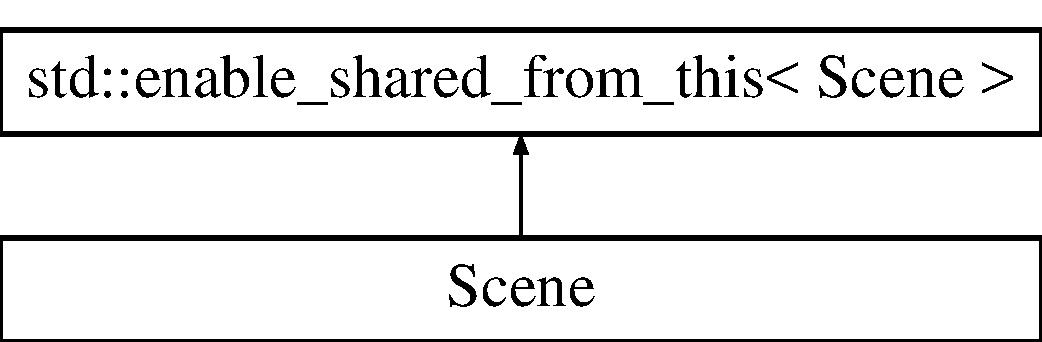
\includegraphics[height=2.000000cm]{class_scene}
\end{center}
\end{figure}
\subsection*{Public Member Functions}
\begin{DoxyCompactItemize}
\item
size\+\_\+t \hyperlink{class_scene_a66108b1261560387be08e2b8226c2237}{Get\+Total\+Objects} () const
\begin{DoxyCompactList}\small\item\em Returns the total number of objects in the scene. \end{DoxyCompactList}\item
size\+\_\+t \hyperlink{class_scene_aca8ac690e36148926c6403d53f5f8527}{Get\+Total\+Lights} () const
\begin{DoxyCompactList}\small\item\em Returns the total number of lights in the scene. \end{DoxyCompactList}\item
{\footnotesize template$<$typename T , typename std\+::enable\+\_\+if$<$ std\+::is\+\_\+integral$<$ T $>$\+::value $>$\+::type $\ast$  = nullptr$>$ }\\const \hyperlink{class_scene_object}{Scene\+Object} \& \hyperlink{class_scene_a643b4969fd3c46d60f1ee8babf8cb5b1}{Get\+Scene\+Object} (T index) const
\begin{DoxyCompactList}\small\item\em Retrive the specified object. \end{DoxyCompactList}\item
{\footnotesize template$<$typename T , typename std\+::enable\+\_\+if$<$ std\+::is\+\_\+integral$<$ T $>$\+::value $>$\+::type $\ast$  = nullptr$>$ }\\const \hyperlink{class_light}{Light} $\ast$ \hyperlink{class_scene_a2dc01d77edcfce9d06fad44a946decf2}{Get\+Light\+Object} (T index) const
\begin{DoxyCompactList}\small\item\em Retrive the specified light. \end{DoxyCompactList}\item
void \hyperlink{class_scene_a6e51f14c74c252d231b73d7109b8117e}{Add\+Scene\+Object} (std\+::shared\+\_\+ptr$<$ \hyperlink{class_scene_object}{Scene\+Object} $>$ object)
\begin{DoxyCompactList}\small\item\em Adds a new object to the scene. \end{DoxyCompactList}\item
void \hyperlink{class_scene_ab9b1a906b16bf867600fc3f5b734c1d4}{Add\+Light} (std\+::shared\+\_\+ptr$<$ \hyperlink{class_light}{Light} $>$ light)
\begin{DoxyCompactList}\small\item\em Adds a new light to the scene. \end{DoxyCompactList}\item
void \hyperlink{class_scene_ac3b0f6126be07f78a61abfac3487e4df}{Clear\+Scene} ()
\begin{DoxyCompactList}\small\item\em Removes all objects and lights from the scene. This prevents them from being rendered. \end{DoxyCompactList}\end{DoxyCompactItemize}
\subsection*{Private Attributes}
\begin{DoxyCompactItemize}
\item
std\+::vector$<$ std\+::shared\+\_\+ptr$<$ \hyperlink{class_scene_object}{Scene\+Object} $>$ $>$ \hyperlink{class_scene_a871382922b2a04d7883cf6d34529b5df}{scene\+Objects}
\item
std\+::vector$<$ std\+::shared\+\_\+ptr$<$ \hyperlink{class_light}{Light} $>$ $>$ \hyperlink{class_scene_a847f4f9c485a56b084a1340811f0e726}{scene\+Lights}
\end{DoxyCompactItemize}
\subsection*{Friends}
\begin{DoxyCompactItemize}
\item
class \hyperlink{class_scene_a70538530bc36e033e360880ef311df61}{Renderer}
\end{DoxyCompactItemize}


\subsection{Detailed Description}
Contains all the objects that need to be rendered as well as the lights.

A \hyperlink{class_scene}{Scene} object functions more or less as a giant container. It stores all the objects and lights that will be used for rendering.

\subsection{Member Function Documentation}
\hypertarget{class_scene_ab9b1a906b16bf867600fc3f5b734c1d4}{}\label{class_scene_ab9b1a906b16bf867600fc3f5b734c1d4}
\index{Scene@{Scene}!Add\+Light@{Add\+Light}}
\index{Add\+Light@{Add\+Light}!Scene@{Scene}}
\subsubsection{\texorpdfstring{Add\+Light()}{AddLight()}}
{\footnotesize\ttfamily void Scene\+::\+Add\+Light (\begin{DoxyParamCaption}\item[{std\+::shared\+\_\+ptr$<$ \hyperlink{class_light}{Light} $>$}]{light }\end{DoxyParamCaption})}



Adds a new light to the scene.


\begin{DoxyParams}{Parameters}
{\em light} & The light to add. \\
\hline
\end{DoxyParams}
\hypertarget{class_scene_a6e51f14c74c252d231b73d7109b8117e}{}\label{class_scene_a6e51f14c74c252d231b73d7109b8117e}
\index{Scene@{Scene}!Add\+Scene\+Object@{Add\+Scene\+Object}}
\index{Add\+Scene\+Object@{Add\+Scene\+Object}!Scene@{Scene}}
\subsubsection{\texorpdfstring{Add\+Scene\+Object()}{AddSceneObject()}}
{\footnotesize\ttfamily void Scene\+::\+Add\+Scene\+Object (\begin{DoxyParamCaption}\item[{std\+::shared\+\_\+ptr$<$ \hyperlink{class_scene_object}{Scene\+Object} $>$}]{object }\end{DoxyParamCaption})}



Adds a new object to the scene.


\begin{DoxyParams}{Parameters}
{\em object} & The object to add. \\
\hline
\end{DoxyParams}
\hypertarget{class_scene_ac3b0f6126be07f78a61abfac3487e4df}{}\label{class_scene_ac3b0f6126be07f78a61abfac3487e4df}
\index{Scene@{Scene}!Clear\+Scene@{Clear\+Scene}}
\index{Clear\+Scene@{Clear\+Scene}!Scene@{Scene}}
\subsubsection{\texorpdfstring{Clear\+Scene()}{ClearScene()}}
{\footnotesize\ttfamily void Scene\+::\+Clear\+Scene (\begin{DoxyParamCaption}{ }\end{DoxyParamCaption})}



Removes all objects and lights from the scene. This prevents them from being rendered.

\hypertarget{class_scene_a2dc01d77edcfce9d06fad44a946decf2}{}\label{class_scene_a2dc01d77edcfce9d06fad44a946decf2}
\index{Scene@{Scene}!Get\+Light\+Object@{Get\+Light\+Object}}
\index{Get\+Light\+Object@{Get\+Light\+Object}!Scene@{Scene}}
\subsubsection{\texorpdfstring{Get\+Light\+Object()}{GetLightObject()}}
{\footnotesize\ttfamily template$<$typename T , typename std\+::enable\+\_\+if$<$ std\+::is\+\_\+integral$<$ T $>$\+::value $>$\+::type $\ast$  = nullptr$>$ \\
const \hyperlink{class_light}{Light}$\ast$ Scene\+::\+Get\+Light\+Object (\begin{DoxyParamCaption}\item[{T}]{index }\end{DoxyParamCaption}) const\hspace{0.3cm}{\ttfamily [inline]}}



Retrive the specified light.


\begin{DoxyParams}{Parameters}
{\em index} & The index to use to access the \hyperlink{class_scene_a847f4f9c485a56b084a1340811f0e726}{Scene\+::scene\+Lights} vector. \\
\hline
\end{DoxyParams}
\begin{DoxyReturn}{Returns}
A pointer to the light in the light vector at the specified index.
\end{DoxyReturn}
Read the \hyperlink{class_scene_a643b4969fd3c46d60f1ee8babf8cb5b1}{Scene\+::\+Get\+Scene\+Object()} docs for more information about std\+::enable\+\_\+if. Note the difference between this function and \hyperlink{class_scene_a643b4969fd3c46d60f1ee8babf8cb5b1}{Scene\+::\+Get\+Scene\+Object()}. Here, if we access the vector out of bounds we return a null pointer, but in \hyperlink{class_scene_a643b4969fd3c46d60f1ee8babf8cb5b1}{Scene\+::\+Get\+Scene\+Object()}, that would be an error. \hypertarget{class_scene_a643b4969fd3c46d60f1ee8babf8cb5b1}{}\label{class_scene_a643b4969fd3c46d60f1ee8babf8cb5b1}
\index{Scene@{Scene}!Get\+Scene\+Object@{Get\+Scene\+Object}}
\index{Get\+Scene\+Object@{Get\+Scene\+Object}!Scene@{Scene}}
\subsubsection{\texorpdfstring{Get\+Scene\+Object()}{GetSceneObject()}}
{\footnotesize\ttfamily template$<$typename T , typename std\+::enable\+\_\+if$<$ std\+::is\+\_\+integral$<$ T $>$\+::value $>$\+::type $\ast$  = nullptr$>$ \\
const \hyperlink{class_scene_object}{Scene\+Object}\& Scene\+::\+Get\+Scene\+Object (\begin{DoxyParamCaption}\item[{T}]{index }\end{DoxyParamCaption}) const\hspace{0.3cm}{\ttfamily [inline]}}



Retrive the specified object.


\begin{DoxyParams}{Parameters}
{\em index} & The index to use to access the \hyperlink{class_scene_a871382922b2a04d7883cf6d34529b5df}{Scene\+::scene\+Objects} vector. \\
\hline
\end{DoxyParams}
\begin{DoxyReturn}{Returns}
A reference to the object in the object vector at the specified index.
\end{DoxyReturn}
Confused about the whole std\+::enable\+\_\+if shenanigans? You can look at the \href{http://en.cppreference.com/w/cpp/types/enable_if}{\tt std\+::enable\+\_\+if} docs. This is part of C++\textquotesingle{}s \href{http://en.cppreference.com/w/cpp/language/sfinae}{\tt S\+F\+I\+N\+AE} rule. Don\textquotesingle{}t worry about it if you don\textquotesingle{}t get most of it. The std\+::enable\+\_\+if is just to make sure that index is an integral (since we want to support int, uint, size\+\_\+t, long, etc.) without casting. \hypertarget{class_scene_aca8ac690e36148926c6403d53f5f8527}{}\label{class_scene_aca8ac690e36148926c6403d53f5f8527}
\index{Scene@{Scene}!Get\+Total\+Lights@{Get\+Total\+Lights}}
\index{Get\+Total\+Lights@{Get\+Total\+Lights}!Scene@{Scene}}
\subsubsection{\texorpdfstring{Get\+Total\+Lights()}{GetTotalLights()}}
{\footnotesize\ttfamily size\+\_\+t Scene\+::\+Get\+Total\+Lights (\begin{DoxyParamCaption}{ }\end{DoxyParamCaption}) const\hspace{0.3cm}{\ttfamily [inline]}}



Returns the total number of lights in the scene.

\begin{DoxyReturn}{Returns}
Total number of lights in the scene.
\end{DoxyReturn}
\hypertarget{class_scene_a66108b1261560387be08e2b8226c2237}{}\label{class_scene_a66108b1261560387be08e2b8226c2237}
\index{Scene@{Scene}!Get\+Total\+Objects@{Get\+Total\+Objects}}
\index{Get\+Total\+Objects@{Get\+Total\+Objects}!Scene@{Scene}}
\subsubsection{\texorpdfstring{Get\+Total\+Objects()}{GetTotalObjects()}}
{\footnotesize\ttfamily size\+\_\+t Scene\+::\+Get\+Total\+Objects (\begin{DoxyParamCaption}{ }\end{DoxyParamCaption}) const\hspace{0.3cm}{\ttfamily [inline]}}



Returns the total number of objects in the scene.

\begin{DoxyReturn}{Returns}
Total number of objects in the scene.
\end{DoxyReturn}


\subsection{Friends And Related Function Documentation}
\hypertarget{class_scene_a70538530bc36e033e360880ef311df61}{}\label{class_scene_a70538530bc36e033e360880ef311df61}
\index{Scene@{Scene}!Renderer@{Renderer}}
\index{Renderer@{Renderer}!Scene@{Scene}}
\subsubsection{\texorpdfstring{Renderer}{Renderer}}
{\footnotesize\ttfamily friend class \hyperlink{class_renderer}{Renderer}\hspace{0.3cm}{\ttfamily [friend]}}



\subsection{Member Data Documentation}
\hypertarget{class_scene_a847f4f9c485a56b084a1340811f0e726}{}\label{class_scene_a847f4f9c485a56b084a1340811f0e726}
\index{Scene@{Scene}!scene\+Lights@{scene\+Lights}}
\index{scene\+Lights@{scene\+Lights}!Scene@{Scene}}
\subsubsection{\texorpdfstring{scene\+Lights}{sceneLights}}
{\footnotesize\ttfamily std\+::vector$<$std\+::shared\+\_\+ptr$<$\hyperlink{class_light}{Light}$>$ $>$ Scene\+::scene\+Lights\hspace{0.3cm}{\ttfamily [private]}}

\hypertarget{class_scene_a871382922b2a04d7883cf6d34529b5df}{}\label{class_scene_a871382922b2a04d7883cf6d34529b5df}
\index{Scene@{Scene}!scene\+Objects@{scene\+Objects}}
\index{scene\+Objects@{scene\+Objects}!Scene@{Scene}}
\subsubsection{\texorpdfstring{scene\+Objects}{sceneObjects}}
{\footnotesize\ttfamily std\+::vector$<$std\+::shared\+\_\+ptr$<$\hyperlink{class_scene_object}{Scene\+Object}$>$ $>$ Scene\+::scene\+Objects\hspace{0.3cm}{\ttfamily [private]}}



The documentation for this class was generated from the following files\+:\begin{DoxyCompactItemize}
\item
/data/MO814A-MC937A/MO814A-MC937Aopengl-\/instructor/source/common/\+Scene/\hyperlink{_scene_8h}{Scene.\+h}\item
/data/MO814A-MC937A/MO814A-MC937Aopengl-\/instructor/source/common/\+Scene/\hyperlink{_scene_8cpp}{Scene.\+cpp}\end{DoxyCompactItemize}

\hypertarget{class_scene_object}{}\section{Scene\+Object Class Reference}
\label{class_scene_object}\index{Scene\+Object@{Scene\+Object}}


Represents a generic object that will live in the 3D world that we call our \hyperlink{class_scene}{Scene}.




{\ttfamily \#include $<$Scene\+Object.\+h$>$}

Inheritance diagram for Scene\+Object\+:\begin{figure}[H]
\begin{center}
\leavevmode
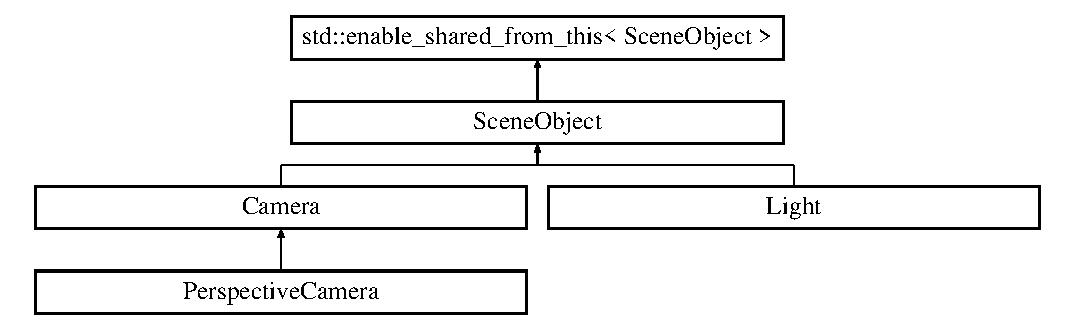
\includegraphics[height=3.985765cm]{class_scene_object}
\end{center}
\end{figure}
\subsection*{Public Member Functions}
\begin{DoxyCompactItemize}
\item
\hyperlink{class_scene_object_a0d268d96d77dbeb45b07a6442e2f4d0d}{Scene\+Object} ()
\begin{DoxyCompactList}\small\item\em Creates an object at the origin, with no rotation, and no scale. \end{DoxyCompactList}\item
\hyperlink{class_scene_object_a9dd76f946c8e0743bed57f9499773fbd}{Scene\+Object} (std\+::shared\+\_\+ptr$<$ class \hyperlink{class_rendering_object}{Rendering\+Object} $>$ base\+Object)
\begin{DoxyCompactList}\small\item\em Creates an object at the origin, with no rotation, and no scale. \end{DoxyCompactList}\item
\hyperlink{class_scene_object_aa89b21b4732296d196a76d1785aee02c}{Scene\+Object} (const std\+::vector$<$ std\+::shared\+\_\+ptr$<$ class \hyperlink{class_rendering_object}{Rendering\+Object} $>$$>$ \&base\+Objects)
\begin{DoxyCompactList}\small\item\em Creates an object at the origin, with no rotation, and no scale. \end{DoxyCompactList}\item
virtual \hyperlink{class_scene_object_ab258d6b94e982d5ae71ad4d7652381f4}{$\sim$\+Scene\+Object} ()
\begin{DoxyCompactList}\small\item\em Destructor. \end{DoxyCompactList}\item
virtual void \hyperlink{class_scene_object_ad516b213a389f6fc57229f65086978ee}{Prepare\+Shader\+For\+Rendering} (const class \hyperlink{class_shader_program}{Shader\+Program} $\ast$shader, const class \hyperlink{class_camera}{Camera} $\ast$current\+Camera, const class \hyperlink{class_light}{Light} $\ast$current\+Light) const
\begin{DoxyCompactList}\small\item\em Passes all uniforms, binds all textures, etc. to the currently bound shader program. \end{DoxyCompactList}\item
size\+\_\+t \hyperlink{class_scene_object_a34f3e11a64d5879def4105b50d853ad1}{Get\+Total\+Render\+Objects} () const
\begin{DoxyCompactList}\small\item\em Returns the total number of rendering objects. \end{DoxyCompactList}\item
virtual const class \hyperlink{class_rendering_object}{Rendering\+Object} $\ast$ \hyperlink{class_scene_object_a0cfa0bb4dbb0f56900ce431cb5dbdda9}{Get\+Render\+Object} (int index=0) const
\begin{DoxyCompactList}\small\item\em Gets the specified rendering object. \end{DoxyCompactList}\item
virtual glm\+::mat4 \hyperlink{class_scene_object_afbb67229fa9895d9e4a9322e64ea4a66}{Get\+Transformation\+Matrix} () const
\begin{DoxyCompactList}\small\item\em Retrieves the current transformation matrix. \end{DoxyCompactList}\item
virtual glm\+::vec4 \hyperlink{class_scene_object_a17a33730106caaeeaede13682440eadc}{Get\+Forward\+Direction} () const
\begin{DoxyCompactList}\small\item\em Computes and returns the forward direction of the object. \end{DoxyCompactList}\item
virtual glm\+::vec4 \hyperlink{class_scene_object_a32985db85bba159afde18da0a16b3934}{Get\+Right\+Direction} () const
\begin{DoxyCompactList}\small\item\em Computes and returns the right direction of the object. \end{DoxyCompactList}\item
virtual glm\+::vec4 \hyperlink{class_scene_object_a88091d7fdb126137d4018738cd30f3d8}{Get\+Up\+Direction} () const
\begin{DoxyCompactList}\small\item\em Computes and returns the up direction of the object. \end{DoxyCompactList}\item
void \hyperlink{class_scene_object_a04868377580069b0ee9d202bdb1b7159}{Translate} (const glm\+::vec3 \&translation)
\begin{DoxyCompactList}\small\item\em Changes the position of the object. \end{DoxyCompactList}\item
void \hyperlink{class_scene_object_a0d27f5853e8e1718b1a77f0f1a6d4551}{Rotate} (const glm\+::vec3 \&axis, float radians)
\begin{DoxyCompactList}\small\item\em Changes the rotation of the object. \end{DoxyCompactList}\item
void \hyperlink{class_scene_object_a00d73ad3f7d77bfc0d3c1869decb97ea}{Mult\+Scale} (float input\+Scale)
\begin{DoxyCompactList}\small\item\em Changes the scale of the object uniformly. \end{DoxyCompactList}\item
void \hyperlink{class_scene_object_a40d7194cf79cad6ee3a2fa7c3d8ed95c}{Add\+Scale} (float input\+Scale)
\begin{DoxyCompactList}\small\item\em Changes the scale of the object uniformly. \end{DoxyCompactList}\item
void \hyperlink{class_scene_object_a1903672e77e88a1e220fcfa8e6afc1d4}{Set\+Position} (const glm\+::vec3 \&in)
\begin{DoxyCompactList}\small\item\em Changes the position of the object. \end{DoxyCompactList}\item
glm\+::vec4 \hyperlink{class_scene_object_a599d20872bfe1f3de5a40dd4535047a5}{Get\+Position} () const
\begin{DoxyCompactList}\small\item\em Gets the position of the object. \end{DoxyCompactList}\end{DoxyCompactItemize}
\subsection*{Static Public Member Functions}
\begin{DoxyCompactItemize}
\item
static glm\+::vec4 \hyperlink{class_scene_object_a334a5fb4e91d85fe6a046bd83dd235d3}{Get\+World\+Up} ()
\begin{DoxyCompactList}\small\item\em The world \textquotesingle{}Up\textquotesingle{} direction. \end{DoxyCompactList}\item
static glm\+::vec4 \hyperlink{class_scene_object_a46d0ffed082f7bd515b9550ef9f9a86a}{Get\+World\+Right} ()
\begin{DoxyCompactList}\small\item\em The world \textquotesingle{}Right\textquotesingle{} direction. \end{DoxyCompactList}\item
static glm\+::vec4 \hyperlink{class_scene_object_a6fa71efda895933be4ee684745980e68}{Get\+World\+Forward} ()
\begin{DoxyCompactList}\small\item\em The world \textquotesingle{}Forward\textquotesingle{} direction. \end{DoxyCompactList}\end{DoxyCompactItemize}
\subsection*{Protected Member Functions}
\begin{DoxyCompactItemize}
\item
virtual void \hyperlink{class_scene_object_a20e31da3f9d2765de50cdb2d637ae6c9}{Update\+Transformation\+Matrix} ()
\begin{DoxyCompactList}\small\item\em Recomputes the cached\+Transformation\+Matrix. \end{DoxyCompactList}\end{DoxyCompactItemize}
\subsection*{Protected Attributes}
\begin{DoxyCompactItemize}
\item
glm\+::mat4 \hyperlink{class_scene_object_aac3f13eea8a7b455e8cffc6eceef211c}{cached\+Transformation\+Matrix}
\item
glm\+::vec4 \hyperlink{class_scene_object_ab4aa9bed778001970c38ea11ef34b285}{position}
\item
glm\+::quat \hyperlink{class_scene_object_ae27376aaca87543a75b5a2cd0daf6e2f}{rotation}
\item
glm\+::vec3 \hyperlink{class_scene_object_a62c686b880fe4f58dec64a409e56de26}{scale}
\end{DoxyCompactItemize}
\subsection*{Static Protected Attributes}
\begin{DoxyCompactItemize}
\item
static const std\+::string \hyperlink{class_scene_object_a62d236f4f5c52b66bd02d13d09b6ce5e}{M\+O\+D\+E\+L\+\_\+\+M\+A\+T\+R\+I\+X\+\_\+\+L\+O\+C\+A\+T\+I\+ON} = \char`\"{}model\+Matrix\char`\"{}
\item
static const std\+::string \hyperlink{class_scene_object_a1c129ecdd6bd8e2f34c713f5dd183361}{V\+I\+E\+W\+\_\+\+M\+A\+T\+R\+I\+X\+\_\+\+L\+O\+C\+A\+T\+I\+ON} = \char`\"{}view\+Matrix\char`\"{}
\item
static const std\+::string \hyperlink{class_scene_object_ad9a8c9c39a4a262c5e379c0bda184541}{P\+R\+O\+J\+E\+C\+T\+I\+O\+N\+\_\+\+M\+A\+T\+R\+I\+X\+\_\+\+L\+O\+C\+A\+T\+I\+ON} = \char`\"{}projection\+Matrix\char`\"{}
\item
static const float \hyperlink{class_scene_object_a903eef54277645571794fd87dc8e9fbb}{M\+I\+N\+I\+M\+U\+M\+\_\+\+S\+C\+A\+LE} = 0.\+01f
\end{DoxyCompactItemize}
\subsection*{Private Attributes}
\begin{DoxyCompactItemize}
\item
std\+::vector$<$ std\+::shared\+\_\+ptr$<$ class \hyperlink{class_rendering_object}{Rendering\+Object} $>$ $>$ \hyperlink{class_scene_object_a4bbf98a19bd8e7ddd491fbb9a41b42cf}{render\+Object}
\end{DoxyCompactItemize}


\subsection{Detailed Description}
Represents a generic object that will live in the 3D world that we call our \hyperlink{class_scene}{Scene}.

Note that this class stores no information about the actual topology of the object. Rather, all it cares about is the relationship between the object space and the world space. The position, rotation, and scale properties all come together to form the \textquotesingle{}model matrix\textquotesingle{} which is just the way of going from object space to world space. Yay math!

\subsection{Constructor \& Destructor Documentation}
\hypertarget{class_scene_object_a0d268d96d77dbeb45b07a6442e2f4d0d}{}\label{class_scene_object_a0d268d96d77dbeb45b07a6442e2f4d0d}
\index{Scene\+Object@{Scene\+Object}!Scene\+Object@{Scene\+Object}}
\index{Scene\+Object@{Scene\+Object}!Scene\+Object@{Scene\+Object}}
\subsubsection{\texorpdfstring{Scene\+Object()}{SceneObject()}\hspace{0.1cm}{\footnotesize\ttfamily [1/3]}}
{\footnotesize\ttfamily Scene\+Object\+::\+Scene\+Object (\begin{DoxyParamCaption}{ }\end{DoxyParamCaption})}



Creates an object at the origin, with no rotation, and no scale.

\hypertarget{class_scene_object_a9dd76f946c8e0743bed57f9499773fbd}{}\label{class_scene_object_a9dd76f946c8e0743bed57f9499773fbd}
\index{Scene\+Object@{Scene\+Object}!Scene\+Object@{Scene\+Object}}
\index{Scene\+Object@{Scene\+Object}!Scene\+Object@{Scene\+Object}}
\subsubsection{\texorpdfstring{Scene\+Object()}{SceneObject()}\hspace{0.1cm}{\footnotesize\ttfamily [2/3]}}
{\footnotesize\ttfamily Scene\+Object\+::\+Scene\+Object (\begin{DoxyParamCaption}\item[{std\+::shared\+\_\+ptr$<$ class \hyperlink{class_rendering_object}{Rendering\+Object} $>$}]{base\+Object }\end{DoxyParamCaption})}



Creates an object at the origin, with no rotation, and no scale.


\begin{DoxyParams}{Parameters}
{\em base\+Object} & The rendering object to associate with this object. \\
\hline
\end{DoxyParams}
\hypertarget{class_scene_object_aa89b21b4732296d196a76d1785aee02c}{}\label{class_scene_object_aa89b21b4732296d196a76d1785aee02c}
\index{Scene\+Object@{Scene\+Object}!Scene\+Object@{Scene\+Object}}
\index{Scene\+Object@{Scene\+Object}!Scene\+Object@{Scene\+Object}}
\subsubsection{\texorpdfstring{Scene\+Object()}{SceneObject()}\hspace{0.1cm}{\footnotesize\ttfamily [3/3]}}
{\footnotesize\ttfamily Scene\+Object\+::\+Scene\+Object (\begin{DoxyParamCaption}\item[{const std\+::vector$<$ std\+::shared\+\_\+ptr$<$ class \hyperlink{class_rendering_object}{Rendering\+Object} $>$$>$ \&}]{base\+Objects }\end{DoxyParamCaption})}



Creates an object at the origin, with no rotation, and no scale.


\begin{DoxyParams}{Parameters}
{\em base\+Objects} & The rendering objects (note\+: plural) to associate with this object. \\
\hline
\end{DoxyParams}
\hypertarget{class_scene_object_ab258d6b94e982d5ae71ad4d7652381f4}{}\label{class_scene_object_ab258d6b94e982d5ae71ad4d7652381f4}
\index{Scene\+Object@{Scene\+Object}!````~Scene\+Object@{$\sim$\+Scene\+Object}}
\index{````~Scene\+Object@{$\sim$\+Scene\+Object}!Scene\+Object@{Scene\+Object}}
\subsubsection{\texorpdfstring{$\sim$\+Scene\+Object()}{~SceneObject()}}
{\footnotesize\ttfamily Scene\+Object\+::$\sim$\+Scene\+Object (\begin{DoxyParamCaption}{ }\end{DoxyParamCaption})\hspace{0.3cm}{\ttfamily [virtual]}}



Destructor.



\subsection{Member Function Documentation}
\hypertarget{class_scene_object_a40d7194cf79cad6ee3a2fa7c3d8ed95c}{}\label{class_scene_object_a40d7194cf79cad6ee3a2fa7c3d8ed95c}
\index{Scene\+Object@{Scene\+Object}!Add\+Scale@{Add\+Scale}}
\index{Add\+Scale@{Add\+Scale}!Scene\+Object@{Scene\+Object}}
\subsubsection{\texorpdfstring{Add\+Scale()}{AddScale()}}
{\footnotesize\ttfamily void Scene\+Object\+::\+Add\+Scale (\begin{DoxyParamCaption}\item[{float}]{input\+Scale }\end{DoxyParamCaption})}



Changes the scale of the object uniformly.


\begin{DoxyParams}{Parameters}
{\em input\+Scale} & The scale to add to the current scale.\\
\hline
\end{DoxyParams}
Let\textquotesingle{}s say the current scale is $(x, x, x)$ and the input scale is $y$ then the final scale is, $(x + y, x + y, x + y)$. \hypertarget{class_scene_object_a17a33730106caaeeaede13682440eadc}{}\label{class_scene_object_a17a33730106caaeeaede13682440eadc}
\index{Scene\+Object@{Scene\+Object}!Get\+Forward\+Direction@{Get\+Forward\+Direction}}
\index{Get\+Forward\+Direction@{Get\+Forward\+Direction}!Scene\+Object@{Scene\+Object}}
\subsubsection{\texorpdfstring{Get\+Forward\+Direction()}{GetForwardDirection()}}
{\footnotesize\ttfamily glm\+::vec4 Scene\+Object\+::\+Get\+Forward\+Direction (\begin{DoxyParamCaption}{ }\end{DoxyParamCaption}) const\hspace{0.3cm}{\ttfamily [virtual]}}



Computes and returns the forward direction of the object.

\begin{DoxyReturn}{Returns}
Returns the forward direction of the object.
\end{DoxyReturn}
Rotates the world forward direction by the object\textquotesingle{}s rotation. \hypertarget{class_scene_object_a599d20872bfe1f3de5a40dd4535047a5}{}\label{class_scene_object_a599d20872bfe1f3de5a40dd4535047a5}
\index{Scene\+Object@{Scene\+Object}!Get\+Position@{Get\+Position}}
\index{Get\+Position@{Get\+Position}!Scene\+Object@{Scene\+Object}}
\subsubsection{\texorpdfstring{Get\+Position()}{GetPosition()}}
{\footnotesize\ttfamily glm\+::vec4 Scene\+Object\+::\+Get\+Position (\begin{DoxyParamCaption}{ }\end{DoxyParamCaption}) const\hspace{0.3cm}{\ttfamily [inline]}}



Gets the position of the object.

\begin{DoxyReturn}{Returns}
The world space position of the object.
\end{DoxyReturn}
\hypertarget{class_scene_object_a0cfa0bb4dbb0f56900ce431cb5dbdda9}{}\label{class_scene_object_a0cfa0bb4dbb0f56900ce431cb5dbdda9}
\index{Scene\+Object@{Scene\+Object}!Get\+Render\+Object@{Get\+Render\+Object}}
\index{Get\+Render\+Object@{Get\+Render\+Object}!Scene\+Object@{Scene\+Object}}
\subsubsection{\texorpdfstring{Get\+Render\+Object()}{GetRenderObject()}}
{\footnotesize\ttfamily const \hyperlink{class_rendering_object}{Rendering\+Object} $\ast$ Scene\+Object\+::\+Get\+Render\+Object (\begin{DoxyParamCaption}\item[{int}]{index = {\ttfamily 0} }\end{DoxyParamCaption}) const\hspace{0.3cm}{\ttfamily [virtual]}}



Gets the specified rendering object.


\begin{DoxyParams}{Parameters}
{\em index} & The index to access in the \hyperlink{class_scene_object_a4bbf98a19bd8e7ddd491fbb9a41b42cf}{Scene\+Object\+::render\+Object} vector. \\
\hline
\end{DoxyParams}
\begin{DoxyReturn}{Returns}
Returns the a pointer to the rendering object at the given index.
\end{DoxyReturn}
If the index access is out of bounds in the vector then a null pointer is returned. \hypertarget{class_scene_object_a32985db85bba159afde18da0a16b3934}{}\label{class_scene_object_a32985db85bba159afde18da0a16b3934}
\index{Scene\+Object@{Scene\+Object}!Get\+Right\+Direction@{Get\+Right\+Direction}}
\index{Get\+Right\+Direction@{Get\+Right\+Direction}!Scene\+Object@{Scene\+Object}}
\subsubsection{\texorpdfstring{Get\+Right\+Direction()}{GetRightDirection()}}
{\footnotesize\ttfamily glm\+::vec4 Scene\+Object\+::\+Get\+Right\+Direction (\begin{DoxyParamCaption}{ }\end{DoxyParamCaption}) const\hspace{0.3cm}{\ttfamily [virtual]}}



Computes and returns the right direction of the object.

\begin{DoxyReturn}{Returns}
Returns the right direction of the object.
\end{DoxyReturn}
Rotates the world right direction by the object\textquotesingle{}s rotation. \hypertarget{class_scene_object_a34f3e11a64d5879def4105b50d853ad1}{}\label{class_scene_object_a34f3e11a64d5879def4105b50d853ad1}
\index{Scene\+Object@{Scene\+Object}!Get\+Total\+Render\+Objects@{Get\+Total\+Render\+Objects}}
\index{Get\+Total\+Render\+Objects@{Get\+Total\+Render\+Objects}!Scene\+Object@{Scene\+Object}}
\subsubsection{\texorpdfstring{Get\+Total\+Render\+Objects()}{GetTotalRenderObjects()}}
{\footnotesize\ttfamily size\+\_\+t Scene\+Object\+::\+Get\+Total\+Render\+Objects (\begin{DoxyParamCaption}{ }\end{DoxyParamCaption}) const\hspace{0.3cm}{\ttfamily [inline]}}



Returns the total number of rendering objects.

\begin{DoxyReturn}{Returns}
The total number of rendering objects.
\end{DoxyReturn}
\hypertarget{class_scene_object_afbb67229fa9895d9e4a9322e64ea4a66}{}\label{class_scene_object_afbb67229fa9895d9e4a9322e64ea4a66}
\index{Scene\+Object@{Scene\+Object}!Get\+Transformation\+Matrix@{Get\+Transformation\+Matrix}}
\index{Get\+Transformation\+Matrix@{Get\+Transformation\+Matrix}!Scene\+Object@{Scene\+Object}}
\subsubsection{\texorpdfstring{Get\+Transformation\+Matrix()}{GetTransformationMatrix()}}
{\footnotesize\ttfamily glm\+::mat4 Scene\+Object\+::\+Get\+Transformation\+Matrix (\begin{DoxyParamCaption}{ }\end{DoxyParamCaption}) const\hspace{0.3cm}{\ttfamily [virtual]}}



Retrieves the current transformation matrix.

\begin{DoxyReturn}{Returns}
\hyperlink{class_scene_object_aac3f13eea8a7b455e8cffc6eceef211c}{Scene\+Object\+::cached\+Transformation\+Matrix}
\end{DoxyReturn}
This function does not perform any computation. Instead, it returns the value of whatever was computed the last time \hyperlink{class_scene_object_a20e31da3f9d2765de50cdb2d637ae6c9}{Update\+Transformation\+Matrix()} was called. \hypertarget{class_scene_object_a88091d7fdb126137d4018738cd30f3d8}{}\label{class_scene_object_a88091d7fdb126137d4018738cd30f3d8}
\index{Scene\+Object@{Scene\+Object}!Get\+Up\+Direction@{Get\+Up\+Direction}}
\index{Get\+Up\+Direction@{Get\+Up\+Direction}!Scene\+Object@{Scene\+Object}}
\subsubsection{\texorpdfstring{Get\+Up\+Direction()}{GetUpDirection()}}
{\footnotesize\ttfamily glm\+::vec4 Scene\+Object\+::\+Get\+Up\+Direction (\begin{DoxyParamCaption}{ }\end{DoxyParamCaption}) const\hspace{0.3cm}{\ttfamily [virtual]}}



Computes and returns the up direction of the object.

\begin{DoxyReturn}{Returns}
Returns the up direction of the object.
\end{DoxyReturn}
Rotates the world up direction by the object\textquotesingle{}s rotation. \hypertarget{class_scene_object_a6fa71efda895933be4ee684745980e68}{}\label{class_scene_object_a6fa71efda895933be4ee684745980e68}
\index{Scene\+Object@{Scene\+Object}!Get\+World\+Forward@{Get\+World\+Forward}}
\index{Get\+World\+Forward@{Get\+World\+Forward}!Scene\+Object@{Scene\+Object}}
\subsubsection{\texorpdfstring{Get\+World\+Forward()}{GetWorldForward()}}
{\footnotesize\ttfamily glm\+::vec4 Scene\+Object\+::\+Get\+World\+Forward (\begin{DoxyParamCaption}{ }\end{DoxyParamCaption})\hspace{0.3cm}{\ttfamily [static]}}



The world \textquotesingle{}Forward\textquotesingle{} direction.

\begin{DoxyReturn}{Returns}
glm\+::vec4(0, 0, -\/1, 0).
\end{DoxyReturn}
\hypertarget{class_scene_object_a46d0ffed082f7bd515b9550ef9f9a86a}{}\label{class_scene_object_a46d0ffed082f7bd515b9550ef9f9a86a}
\index{Scene\+Object@{Scene\+Object}!Get\+World\+Right@{Get\+World\+Right}}
\index{Get\+World\+Right@{Get\+World\+Right}!Scene\+Object@{Scene\+Object}}
\subsubsection{\texorpdfstring{Get\+World\+Right()}{GetWorldRight()}}
{\footnotesize\ttfamily glm\+::vec4 Scene\+Object\+::\+Get\+World\+Right (\begin{DoxyParamCaption}{ }\end{DoxyParamCaption})\hspace{0.3cm}{\ttfamily [static]}}



The world \textquotesingle{}Right\textquotesingle{} direction.

\begin{DoxyReturn}{Returns}
glm\+::vec4(1, 0, 0, 0).
\end{DoxyReturn}
\hypertarget{class_scene_object_a334a5fb4e91d85fe6a046bd83dd235d3}{}\label{class_scene_object_a334a5fb4e91d85fe6a046bd83dd235d3}
\index{Scene\+Object@{Scene\+Object}!Get\+World\+Up@{Get\+World\+Up}}
\index{Get\+World\+Up@{Get\+World\+Up}!Scene\+Object@{Scene\+Object}}
\subsubsection{\texorpdfstring{Get\+World\+Up()}{GetWorldUp()}}
{\footnotesize\ttfamily glm\+::vec4 Scene\+Object\+::\+Get\+World\+Up (\begin{DoxyParamCaption}{ }\end{DoxyParamCaption})\hspace{0.3cm}{\ttfamily [static]}}



The world \textquotesingle{}Up\textquotesingle{} direction.

\begin{DoxyReturn}{Returns}
glm\+::vec4(0, 1, 0, 0).
\end{DoxyReturn}
\hypertarget{class_scene_object_a00d73ad3f7d77bfc0d3c1869decb97ea}{}\label{class_scene_object_a00d73ad3f7d77bfc0d3c1869decb97ea}
\index{Scene\+Object@{Scene\+Object}!Mult\+Scale@{Mult\+Scale}}
\index{Mult\+Scale@{Mult\+Scale}!Scene\+Object@{Scene\+Object}}
\subsubsection{\texorpdfstring{Mult\+Scale()}{MultScale()}}
{\footnotesize\ttfamily void Scene\+Object\+::\+Mult\+Scale (\begin{DoxyParamCaption}\item[{float}]{input\+Scale }\end{DoxyParamCaption})}



Changes the scale of the object uniformly.


\begin{DoxyParams}{Parameters}
{\em input\+Scale} & The scale to multiply to the current scale.\\
\hline
\end{DoxyParams}
Let\textquotesingle{}s say the current scale is $(x, x, x)$ and the input scale is $y$ then the final scale is, $(xy, xy, xy)$. \hypertarget{class_scene_object_ad516b213a389f6fc57229f65086978ee}{}\label{class_scene_object_ad516b213a389f6fc57229f65086978ee}
\index{Scene\+Object@{Scene\+Object}!Prepare\+Shader\+For\+Rendering@{Prepare\+Shader\+For\+Rendering}}
\index{Prepare\+Shader\+For\+Rendering@{Prepare\+Shader\+For\+Rendering}!Scene\+Object@{Scene\+Object}}
\subsubsection{\texorpdfstring{Prepare\+Shader\+For\+Rendering()}{PrepareShaderForRendering()}}
{\footnotesize\ttfamily void Scene\+Object\+::\+Prepare\+Shader\+For\+Rendering (\begin{DoxyParamCaption}\item[{const class \hyperlink{class_shader_program}{Shader\+Program} $\ast$}]{shader,  }\item[{const class \hyperlink{class_camera}{Camera} $\ast$}]{current\+Camera,  }\item[{const class \hyperlink{class_light}{Light} $\ast$}]{current\+Light }\end{DoxyParamCaption}) const\hspace{0.3cm}{\ttfamily [virtual]}}



Passes all uniforms, binds all textures, etc. to the currently bound shader program.


\begin{DoxyParams}{Parameters}
{\em shader} & The shader program to use. \\
\hline
{\em current\+Camera} & The current camera to use. \\
\hline
{\em current\+Light} & The current light to use.\\
\hline
\end{DoxyParams}
Note that this assumes that the shader will only depend on five things\+:
\begin{DoxyItemize}
\item The material stored in the shader.
\item The passed in camera.
\item The passed in light.
\item The current object\textquotesingle{}s orientation in world space.
\item The topology of the various meshes stored in the rendering object (not handled in this function). This function will personally take care of writing the M\+VP matrices to the shader, but will let the shader object itself handle processing its necessary camera and light properties.
\end{DoxyItemize}\hypertarget{class_scene_object_a0d27f5853e8e1718b1a77f0f1a6d4551}{}\label{class_scene_object_a0d27f5853e8e1718b1a77f0f1a6d4551}
\index{Scene\+Object@{Scene\+Object}!Rotate@{Rotate}}
\index{Rotate@{Rotate}!Scene\+Object@{Scene\+Object}}
\subsubsection{\texorpdfstring{Rotate()}{Rotate()}}
{\footnotesize\ttfamily void Scene\+Object\+::\+Rotate (\begin{DoxyParamCaption}\item[{const glm\+::vec3 \&}]{axis,  }\item[{float}]{radians }\end{DoxyParamCaption})}



Changes the rotation of the object.


\begin{DoxyParams}{Parameters}
{\em axis} & The axis to rotate around. \\
\hline
{\em radians} & The number of radians to rotate around the axis. \\
\hline
\end{DoxyParams}
\hypertarget{class_scene_object_a1903672e77e88a1e220fcfa8e6afc1d4}{}\label{class_scene_object_a1903672e77e88a1e220fcfa8e6afc1d4}
\index{Scene\+Object@{Scene\+Object}!Set\+Position@{Set\+Position}}
\index{Set\+Position@{Set\+Position}!Scene\+Object@{Scene\+Object}}
\subsubsection{\texorpdfstring{Set\+Position()}{SetPosition()}}
{\footnotesize\ttfamily void Scene\+Object\+::\+Set\+Position (\begin{DoxyParamCaption}\item[{const glm\+::vec3 \&}]{in }\end{DoxyParamCaption})}



Changes the position of the object.


\begin{DoxyParams}{Parameters}
{\em in} & The new position of the object. \\
\hline
\end{DoxyParams}
\hypertarget{class_scene_object_a04868377580069b0ee9d202bdb1b7159}{}\label{class_scene_object_a04868377580069b0ee9d202bdb1b7159}
\index{Scene\+Object@{Scene\+Object}!Translate@{Translate}}
\index{Translate@{Translate}!Scene\+Object@{Scene\+Object}}
\subsubsection{\texorpdfstring{Translate()}{Translate()}}
{\footnotesize\ttfamily void Scene\+Object\+::\+Translate (\begin{DoxyParamCaption}\item[{const glm\+::vec3 \&}]{translation }\end{DoxyParamCaption})}



Changes the position of the object.


\begin{DoxyParams}{Parameters}
{\em translation} & The world space translation to give to the object. \\
\hline
\end{DoxyParams}
\hypertarget{class_scene_object_a20e31da3f9d2765de50cdb2d637ae6c9}{}\label{class_scene_object_a20e31da3f9d2765de50cdb2d637ae6c9}
\index{Scene\+Object@{Scene\+Object}!Update\+Transformation\+Matrix@{Update\+Transformation\+Matrix}}
\index{Update\+Transformation\+Matrix@{Update\+Transformation\+Matrix}!Scene\+Object@{Scene\+Object}}
\subsubsection{\texorpdfstring{Update\+Transformation\+Matrix()}{UpdateTransformationMatrix()}}
{\footnotesize\ttfamily void Scene\+Object\+::\+Update\+Transformation\+Matrix (\begin{DoxyParamCaption}{ }\end{DoxyParamCaption})\hspace{0.3cm}{\ttfamily [protected]}, {\ttfamily [virtual]}}



Recomputes the cached\+Transformation\+Matrix.

This function should be called whenever you need the cached\+Transformation\+Matrix and there has been a change in the position, rotation, or scale of an object. Currently it is called every time \hyperlink{class_scene_object_a04868377580069b0ee9d202bdb1b7159}{Translate()}, \hyperlink{class_scene_object_a0d27f5853e8e1718b1a77f0f1a6d4551}{Rotate()}, \hyperlink{class_scene_object_a00d73ad3f7d77bfc0d3c1869decb97ea}{Mult\+Scale()}, \hyperlink{class_scene_object_a40d7194cf79cad6ee3a2fa7c3d8ed95c}{Add\+Scale()}, and \hyperlink{class_scene_object_a1903672e77e88a1e220fcfa8e6afc1d4}{Set\+Position()} are called; however, it would be more efficient to only call it once per frame right before the render call.

Reimplemented in \hyperlink{class_perspective_camera_a2f17fb07425e2146d5692805753fa368}{Perspective\+Camera}, and \hyperlink{class_camera_aea640c892a3807671d8ca49616d96eda}{Camera}.



\subsection{Member Data Documentation}
\hypertarget{class_scene_object_aac3f13eea8a7b455e8cffc6eceef211c}{}\label{class_scene_object_aac3f13eea8a7b455e8cffc6eceef211c}
\index{Scene\+Object@{Scene\+Object}!cached\+Transformation\+Matrix@{cached\+Transformation\+Matrix}}
\index{cached\+Transformation\+Matrix@{cached\+Transformation\+Matrix}!Scene\+Object@{Scene\+Object}}
\subsubsection{\texorpdfstring{cached\+Transformation\+Matrix}{cachedTransformationMatrix}}
{\footnotesize\ttfamily glm\+::mat4 Scene\+Object\+::cached\+Transformation\+Matrix\hspace{0.3cm}{\ttfamily [protected]}}

\hypertarget{class_scene_object_a903eef54277645571794fd87dc8e9fbb}{}\label{class_scene_object_a903eef54277645571794fd87dc8e9fbb}
\index{Scene\+Object@{Scene\+Object}!M\+I\+N\+I\+M\+U\+M\+\_\+\+S\+C\+A\+LE@{M\+I\+N\+I\+M\+U\+M\+\_\+\+S\+C\+A\+LE}}
\index{M\+I\+N\+I\+M\+U\+M\+\_\+\+S\+C\+A\+LE@{M\+I\+N\+I\+M\+U\+M\+\_\+\+S\+C\+A\+LE}!Scene\+Object@{Scene\+Object}}
\subsubsection{\texorpdfstring{M\+I\+N\+I\+M\+U\+M\+\_\+\+S\+C\+A\+LE}{MINIMUM\_SCALE}}
{\footnotesize\ttfamily const float Scene\+Object\+::\+M\+I\+N\+I\+M\+U\+M\+\_\+\+S\+C\+A\+LE = 0.\+01f\hspace{0.3cm}{\ttfamily [static]}, {\ttfamily [protected]}}

\hypertarget{class_scene_object_a62d236f4f5c52b66bd02d13d09b6ce5e}{}\label{class_scene_object_a62d236f4f5c52b66bd02d13d09b6ce5e}
\index{Scene\+Object@{Scene\+Object}!M\+O\+D\+E\+L\+\_\+\+M\+A\+T\+R\+I\+X\+\_\+\+L\+O\+C\+A\+T\+I\+ON@{M\+O\+D\+E\+L\+\_\+\+M\+A\+T\+R\+I\+X\+\_\+\+L\+O\+C\+A\+T\+I\+ON}}
\index{M\+O\+D\+E\+L\+\_\+\+M\+A\+T\+R\+I\+X\+\_\+\+L\+O\+C\+A\+T\+I\+ON@{M\+O\+D\+E\+L\+\_\+\+M\+A\+T\+R\+I\+X\+\_\+\+L\+O\+C\+A\+T\+I\+ON}!Scene\+Object@{Scene\+Object}}
\subsubsection{\texorpdfstring{M\+O\+D\+E\+L\+\_\+\+M\+A\+T\+R\+I\+X\+\_\+\+L\+O\+C\+A\+T\+I\+ON}{MODEL\_MATRIX\_LOCATION}}
{\footnotesize\ttfamily const std\+::string Scene\+Object\+::\+M\+O\+D\+E\+L\+\_\+\+M\+A\+T\+R\+I\+X\+\_\+\+L\+O\+C\+A\+T\+I\+ON = \char`\"{}model\+Matrix\char`\"{}\hspace{0.3cm}{\ttfamily [static]}, {\ttfamily [protected]}}

\hypertarget{class_scene_object_ab4aa9bed778001970c38ea11ef34b285}{}\label{class_scene_object_ab4aa9bed778001970c38ea11ef34b285}
\index{Scene\+Object@{Scene\+Object}!position@{position}}
\index{position@{position}!Scene\+Object@{Scene\+Object}}
\subsubsection{\texorpdfstring{position}{position}}
{\footnotesize\ttfamily glm\+::vec4 Scene\+Object\+::position\hspace{0.3cm}{\ttfamily [protected]}}

\hypertarget{class_scene_object_ad9a8c9c39a4a262c5e379c0bda184541}{}\label{class_scene_object_ad9a8c9c39a4a262c5e379c0bda184541}
\index{Scene\+Object@{Scene\+Object}!P\+R\+O\+J\+E\+C\+T\+I\+O\+N\+\_\+\+M\+A\+T\+R\+I\+X\+\_\+\+L\+O\+C\+A\+T\+I\+ON@{P\+R\+O\+J\+E\+C\+T\+I\+O\+N\+\_\+\+M\+A\+T\+R\+I\+X\+\_\+\+L\+O\+C\+A\+T\+I\+ON}}
\index{P\+R\+O\+J\+E\+C\+T\+I\+O\+N\+\_\+\+M\+A\+T\+R\+I\+X\+\_\+\+L\+O\+C\+A\+T\+I\+ON@{P\+R\+O\+J\+E\+C\+T\+I\+O\+N\+\_\+\+M\+A\+T\+R\+I\+X\+\_\+\+L\+O\+C\+A\+T\+I\+ON}!Scene\+Object@{Scene\+Object}}
\subsubsection{\texorpdfstring{P\+R\+O\+J\+E\+C\+T\+I\+O\+N\+\_\+\+M\+A\+T\+R\+I\+X\+\_\+\+L\+O\+C\+A\+T\+I\+ON}{PROJECTION\_MATRIX\_LOCATION}}
{\footnotesize\ttfamily const std\+::string Scene\+Object\+::\+P\+R\+O\+J\+E\+C\+T\+I\+O\+N\+\_\+\+M\+A\+T\+R\+I\+X\+\_\+\+L\+O\+C\+A\+T\+I\+ON = \char`\"{}projection\+Matrix\char`\"{}\hspace{0.3cm}{\ttfamily [static]}, {\ttfamily [protected]}}

\hypertarget{class_scene_object_a4bbf98a19bd8e7ddd491fbb9a41b42cf}{}\label{class_scene_object_a4bbf98a19bd8e7ddd491fbb9a41b42cf}
\index{Scene\+Object@{Scene\+Object}!render\+Object@{render\+Object}}
\index{render\+Object@{render\+Object}!Scene\+Object@{Scene\+Object}}
\subsubsection{\texorpdfstring{render\+Object}{renderObject}}
{\footnotesize\ttfamily std\+::vector$<$std\+::shared\+\_\+ptr$<$class \hyperlink{class_rendering_object}{Rendering\+Object}$>$ $>$ Scene\+Object\+::render\+Object\hspace{0.3cm}{\ttfamily [private]}}

\hypertarget{class_scene_object_ae27376aaca87543a75b5a2cd0daf6e2f}{}\label{class_scene_object_ae27376aaca87543a75b5a2cd0daf6e2f}
\index{Scene\+Object@{Scene\+Object}!rotation@{rotation}}
\index{rotation@{rotation}!Scene\+Object@{Scene\+Object}}
\subsubsection{\texorpdfstring{rotation}{rotation}}
{\footnotesize\ttfamily glm\+::quat Scene\+Object\+::rotation\hspace{0.3cm}{\ttfamily [protected]}}

\hypertarget{class_scene_object_a62c686b880fe4f58dec64a409e56de26}{}\label{class_scene_object_a62c686b880fe4f58dec64a409e56de26}
\index{Scene\+Object@{Scene\+Object}!scale@{scale}}
\index{scale@{scale}!Scene\+Object@{Scene\+Object}}
\subsubsection{\texorpdfstring{scale}{scale}}
{\footnotesize\ttfamily glm\+::vec3 Scene\+Object\+::scale\hspace{0.3cm}{\ttfamily [protected]}}

\hypertarget{class_scene_object_a1c129ecdd6bd8e2f34c713f5dd183361}{}\label{class_scene_object_a1c129ecdd6bd8e2f34c713f5dd183361}
\index{Scene\+Object@{Scene\+Object}!V\+I\+E\+W\+\_\+\+M\+A\+T\+R\+I\+X\+\_\+\+L\+O\+C\+A\+T\+I\+ON@{V\+I\+E\+W\+\_\+\+M\+A\+T\+R\+I\+X\+\_\+\+L\+O\+C\+A\+T\+I\+ON}}
\index{V\+I\+E\+W\+\_\+\+M\+A\+T\+R\+I\+X\+\_\+\+L\+O\+C\+A\+T\+I\+ON@{V\+I\+E\+W\+\_\+\+M\+A\+T\+R\+I\+X\+\_\+\+L\+O\+C\+A\+T\+I\+ON}!Scene\+Object@{Scene\+Object}}
\subsubsection{\texorpdfstring{V\+I\+E\+W\+\_\+\+M\+A\+T\+R\+I\+X\+\_\+\+L\+O\+C\+A\+T\+I\+ON}{VIEW\_MATRIX\_LOCATION}}
{\footnotesize\ttfamily const std\+::string Scene\+Object\+::\+V\+I\+E\+W\+\_\+\+M\+A\+T\+R\+I\+X\+\_\+\+L\+O\+C\+A\+T\+I\+ON = \char`\"{}view\+Matrix\char`\"{}\hspace{0.3cm}{\ttfamily [static]}, {\ttfamily [protected]}}



The documentation for this class was generated from the following files\+:\begin{DoxyCompactItemize}
\item
/data/MO814A-MC937A/MO814A-MC937Aopengl-\/instructor/source/common/\+Scene/\hyperlink{_scene_object_8h}{Scene\+Object.\+h}\item
/data/MO814A-MC937A/MO814A-MC937Aopengl-\/instructor/source/common/\+Scene/\hyperlink{_scene_object_8cpp}{Scene\+Object.\+cpp}\end{DoxyCompactItemize}

\hypertarget{class_shader_program}{}\section{Shader\+Program Class Reference}
\label{class_shader_program}\index{Shader\+Program@{Shader\+Program}}


Interfaces with the underlying G\+L\+SL shader program.




{\ttfamily \#include $<$Shader\+Program.\+h$>$}

Inheritance diagram for Shader\+Program\+:\begin{figure}[H]
\begin{center}
\leavevmode
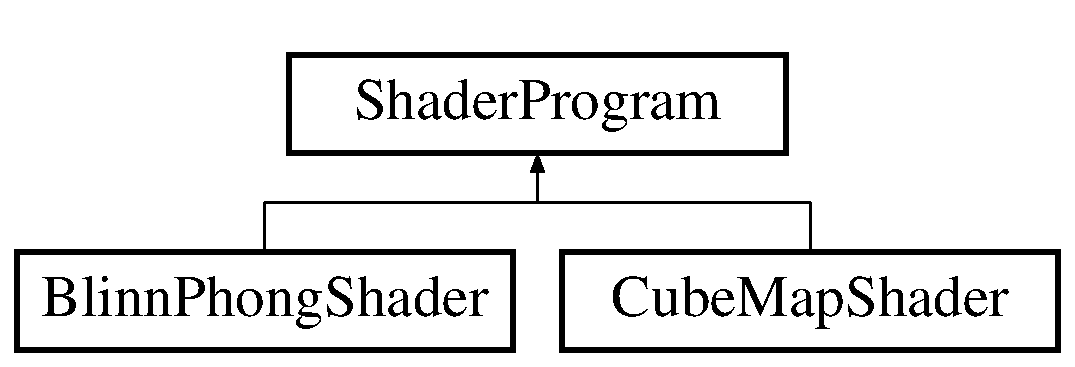
\includegraphics[height=2.000000cm]{class_shader_program}
\end{center}
\end{figure}
\subsection*{Public Member Functions}
\begin{DoxyCompactItemize}
\item
\hyperlink{class_shader_program_aba2db5734b2f70cc34078126ad279588}{Shader\+Program} (const std\+::unordered\+\_\+map$<$ G\+Lenum, std\+::string $>$ \&input\+Shaders)
\begin{DoxyCompactList}\small\item\em Creates a shader program. \end{DoxyCompactList}\item
virtual void \hyperlink{class_shader_program_a51ac6fbf3a3d88643eef303a4c3a1fa8}{Load\+Material\+From\+Assimp} (std\+::shared\+\_\+ptr$<$ struct ai\+Material $>$ assimp\+Material)
\item
virtual \hyperlink{class_shader_program_a2d2eadcfc48cc2e2ddb82aba70553a9f}{$\sim$\+Shader\+Program} ()
\begin{DoxyCompactList}\small\item\em A destructor to clean up the shader program. \end{DoxyCompactList}\item
virtual void \hyperlink{class_shader_program_aab1241c0f0962d43687d92866d7b7d6a}{Start\+Use\+Shader} () const
\begin{DoxyCompactList}\small\item\em Notifies the Open\+GL state that we will be using the underlying G\+L\+SL program. \end{DoxyCompactList}\item
virtual void \hyperlink{class_shader_program_a2f2ae9ab4849f855becccfaa445d00d5}{Stop\+Use\+Shader} () const
\begin{DoxyCompactList}\small\item\em Tells the Open\+GL state to no longer us the underlying shader. \end{DoxyCompactList}\item
G\+Luint \hyperlink{class_shader_program_a7313b3596bcd6d982d9624a46cc2acc6}{Get\+Program} () const
\begin{DoxyCompactList}\small\item\em Gets the underlying shader program identifier created by \href{https://www.opengl.org/sdk/docs/man/html/glCreateProgram.xhtml}{\tt gl\+Create\+Program}. \end{DoxyCompactList}\item
virtual void \hyperlink{class_shader_program_a02cf3df43c59808160fce158ad655a40}{Setup\+Shader\+Lighting} (const class \hyperlink{class_light}{Light} $\ast$light) const
\begin{DoxyCompactList}\small\item\em This function will pass to the G\+L\+SL shader the variables needed by the shader to accurately shade the model using the given light. \end{DoxyCompactList}\item
virtual void \hyperlink{class_shader_program_a20ea5669f122fa6143e7fa8ee9d92578}{Setup\+Shader\+Materials} () const
\begin{DoxyCompactList}\small\item\em Sets up the shader material (what this material is depends on the shader). \end{DoxyCompactList}\item
virtual void \hyperlink{class_shader_program_abefd4e66aae75993f05bd607b6b0ed22}{Setup\+Shader\+Camera} (const class \hyperlink{class_camera}{Camera} $\ast$camera) const
\begin{DoxyCompactList}\small\item\em Passes camera parameters to the shader if necessary. \end{DoxyCompactList}\item
void \hyperlink{class_shader_program_a84ff179a393c8dcd55c38eef19925fef}{Set\+Shader\+Uniform} (const std\+::string \&location, const glm\+::mat4 \&value) const
\begin{DoxyCompactList}\small\item\em Sets a shader uniform with a mat4x4 value. \end{DoxyCompactList}\item
void \hyperlink{class_shader_program_a7ffbc023f4bb3ae2c8b458eb7182dff0}{Set\+Shader\+Uniform} (const std\+::string \&location, float value) const
\begin{DoxyCompactList}\small\item\em Sets a shader uniform with a float value. \end{DoxyCompactList}\item
void \hyperlink{class_shader_program_a16164eb7e3f1e2ca9bf60c492e43b4df}{Set\+Shader\+Uniform} (const std\+::string \&location, int value) const
\begin{DoxyCompactList}\small\item\em Sets a shader uniform with a int value. \end{DoxyCompactList}\item
void \hyperlink{class_shader_program_a5138c3a38a576bbb90d37ab8be6395bf}{Set\+Shader\+Uniform} (const std\+::string \&location, const glm\+::vec4 \&value) const
\begin{DoxyCompactList}\small\item\em Sets a shader uniform with a vec4 value. \end{DoxyCompactList}\item
void \hyperlink{class_shader_program_a00815a3efc74c4ff9a12f2a0c9b46d6e}{Set\+Shader\+Subroutine} (const std\+::string \&location, const std\+::string \&subroutine, G\+Lenum substage) const
\begin{DoxyCompactList}\small\item\em Sets a shader subroutine variable to point to the desired subroutine. \end{DoxyCompactList}\item
{\footnotesize template$<$int N$>$ }\\void \hyperlink{class_shader_program_aac2a462281a872df0ed8d197ec0b4104}{Setup\+Uniform\+Block} (const std\+::string \&block\+Name, std\+::array$<$ const char $\ast$, N $>$ \&names, std\+::array$<$ G\+Luint, N $>$ \&indices, std\+::array$<$ G\+Lint, N $>$ \&offsets, std\+::vector$<$ G\+Lubyte $>$ \&data, G\+Luint \&block\+Location, G\+Lint \&block\+Size, G\+Luint \&buffer\+Location)
\begin{DoxyCompactList}\small\item\em Sets up a shader uniform block with N variables. \end{DoxyCompactList}\item
virtual bool \hyperlink{class_shader_program_a20b5ed7b5f81154025eb7b6f1be70f84}{Is\+Affected\+By\+Light} (const class \hyperlink{class_light}{Light} $\ast$light) const
\end{DoxyCompactItemize}
\subsection*{Static Protected Member Functions}
\begin{DoxyCompactItemize}
\item
static G\+Luint \hyperlink{class_shader_program_ab5c50c33203cf65b7f6ffe00d2243d5a}{Load\+Shader\+Object} (G\+Lenum type, const std\+::string \&filename)
\begin{DoxyCompactList}\small\item\em Reads in a shader object and returns the Open\+GL shader object name. \end{DoxyCompactList}\end{DoxyCompactItemize}
\subsection*{Protected Attributes}
\begin{DoxyCompactItemize}
\item
G\+Luint \hyperlink{class_shader_program_a7d8f2b643a81ac4097606e43ade92f81}{shader\+Program}
\end{DoxyCompactItemize}
\subsection*{Private Attributes}
\begin{DoxyCompactItemize}
\item
std\+::unordered\+\_\+map$<$ G\+Lenum, G\+Luint $>$ \hyperlink{class_shader_program_a8eabcc4ff693bc9430daef8cfc6008de}{shader\+Objects}
\end{DoxyCompactItemize}
\subsection*{Static Private Attributes}
\begin{DoxyCompactItemize}
\item
static const int \hyperlink{class_shader_program_a8839da24bcba7d96ce590146523a8d47}{S\+H\+A\+D\+E\+R\+\_\+\+E\+R\+R\+O\+R\+\_\+\+L\+O\+G\+\_\+\+S\+I\+ZE} = 500
\end{DoxyCompactItemize}


\subsection{Detailed Description}
Interfaces with the underlying G\+L\+SL shader program.

This class wil manage the G\+L\+SL shader program from loading and compiling to setting runtime variables. The shader interfaces closely with the underlying shader especially in \hyperlink{class_shader_program_a02cf3df43c59808160fce158ad655a40}{Shader\+Program\+::\+Setup\+Shader\+Lighting()}, \hyperlink{class_shader_program_a20ea5669f122fa6143e7fa8ee9d92578}{Shader\+Program\+::\+Setup\+Shader\+Materials()}, and \hyperlink{class_shader_program_abefd4e66aae75993f05bd607b6b0ed22}{Shader\+Program\+::\+Setup\+Shader\+Camera()}. This class (and its subclasses) will directly correspond to a shader program (vertex shader plus a fragment shader). So if you ever decide to create a new type of shader (not the provided Blinn-\/\+Phong one), you will have to create a new sub-\/class of \hyperlink{class_shader_program}{Shader\+Program} to make sure that its uniforms are setup properly.

\subsection{Constructor \& Destructor Documentation}
\hypertarget{class_shader_program_aba2db5734b2f70cc34078126ad279588}{}\label{class_shader_program_aba2db5734b2f70cc34078126ad279588}
\index{Shader\+Program@{Shader\+Program}!Shader\+Program@{Shader\+Program}}
\index{Shader\+Program@{Shader\+Program}!Shader\+Program@{Shader\+Program}}
\subsubsection{\texorpdfstring{Shader\+Program()}{ShaderProgram()}}
{\footnotesize\ttfamily Shader\+Program\+::\+Shader\+Program (\begin{DoxyParamCaption}\item[{const std\+::unordered\+\_\+map$<$ G\+Lenum, std\+::string $>$ \&}]{input\+Shaders }\end{DoxyParamCaption})}



Creates a shader program.


\begin{DoxyParams}{Parameters}
{\em input\+Shaders} & A map of the shader type to the shader file location.\\
\hline
\end{DoxyParams}
At the minimum a vertex shader is required to create a G\+L\+SL shader program; however, using a fragment shader is highly recommended unless you know what you are doing. \hypertarget{class_shader_program_a2d2eadcfc48cc2e2ddb82aba70553a9f}{}\label{class_shader_program_a2d2eadcfc48cc2e2ddb82aba70553a9f}
\index{Shader\+Program@{Shader\+Program}!````~Shader\+Program@{$\sim$\+Shader\+Program}}
\index{````~Shader\+Program@{$\sim$\+Shader\+Program}!Shader\+Program@{Shader\+Program}}
\subsubsection{\texorpdfstring{$\sim$\+Shader\+Program()}{~ShaderProgram()}}
{\footnotesize\ttfamily Shader\+Program\+::$\sim$\+Shader\+Program (\begin{DoxyParamCaption}{ }\end{DoxyParamCaption})\hspace{0.3cm}{\ttfamily [virtual]}}



A destructor to clean up the shader program.



\subsection{Member Function Documentation}
\hypertarget{class_shader_program_a7313b3596bcd6d982d9624a46cc2acc6}{}\label{class_shader_program_a7313b3596bcd6d982d9624a46cc2acc6}
\index{Shader\+Program@{Shader\+Program}!Get\+Program@{Get\+Program}}
\index{Get\+Program@{Get\+Program}!Shader\+Program@{Shader\+Program}}
\subsubsection{\texorpdfstring{Get\+Program()}{GetProgram()}}
{\footnotesize\ttfamily G\+Luint Shader\+Program\+::\+Get\+Program (\begin{DoxyParamCaption}{ }\end{DoxyParamCaption}) const\hspace{0.3cm}{\ttfamily [inline]}}



Gets the underlying shader program identifier created by \href{https://www.opengl.org/sdk/docs/man/html/glCreateProgram.xhtml}{\tt gl\+Create\+Program}.

\begin{DoxyReturn}{Returns}
The shader program identifier created by \href{https://www.opengl.org/sdk/docs/man/html/glCreateProgram.xhtml}{\tt gl\+Create\+Program}.
\end{DoxyReturn}
\hypertarget{class_shader_program_a20b5ed7b5f81154025eb7b6f1be70f84}{}\label{class_shader_program_a20b5ed7b5f81154025eb7b6f1be70f84}
\index{Shader\+Program@{Shader\+Program}!Is\+Affected\+By\+Light@{Is\+Affected\+By\+Light}}
\index{Is\+Affected\+By\+Light@{Is\+Affected\+By\+Light}!Shader\+Program@{Shader\+Program}}
\subsubsection{\texorpdfstring{Is\+Affected\+By\+Light()}{IsAffectedByLight()}}
{\footnotesize\ttfamily virtual bool Shader\+Program\+::\+Is\+Affected\+By\+Light (\begin{DoxyParamCaption}\item[{const class \hyperlink{class_light}{Light} $\ast$}]{light }\end{DoxyParamCaption}) const\hspace{0.3cm}{\ttfamily [inline]}, {\ttfamily [virtual]}}



Reimplemented in \hyperlink{class_cube_map_shader_aa0c9e535cb18663acd9857165abc788f}{Cube\+Map\+Shader}.

\hypertarget{class_shader_program_a51ac6fbf3a3d88643eef303a4c3a1fa8}{}\label{class_shader_program_a51ac6fbf3a3d88643eef303a4c3a1fa8}
\index{Shader\+Program@{Shader\+Program}!Load\+Material\+From\+Assimp@{Load\+Material\+From\+Assimp}}
\index{Load\+Material\+From\+Assimp@{Load\+Material\+From\+Assimp}!Shader\+Program@{Shader\+Program}}
\subsubsection{\texorpdfstring{Load\+Material\+From\+Assimp()}{LoadMaterialFromAssimp()}}
{\footnotesize\ttfamily virtual void Shader\+Program\+::\+Load\+Material\+From\+Assimp (\begin{DoxyParamCaption}\item[{std\+::shared\+\_\+ptr$<$ struct ai\+Material $>$}]{assimp\+Material }\end{DoxyParamCaption})\hspace{0.3cm}{\ttfamily [inline]}, {\ttfamily [virtual]}}



Reimplemented in \hyperlink{class_blinn_phong_shader_a5a2a720a403f3d005b07a96fee35b95b}{Blinn\+Phong\+Shader}.

\hypertarget{class_shader_program_ab5c50c33203cf65b7f6ffe00d2243d5a}{}\label{class_shader_program_ab5c50c33203cf65b7f6ffe00d2243d5a}
\index{Shader\+Program@{Shader\+Program}!Load\+Shader\+Object@{Load\+Shader\+Object}}
\index{Load\+Shader\+Object@{Load\+Shader\+Object}!Shader\+Program@{Shader\+Program}}
\subsubsection{\texorpdfstring{Load\+Shader\+Object()}{LoadShaderObject()}}
{\footnotesize\ttfamily G\+Luint Shader\+Program\+::\+Load\+Shader\+Object (\begin{DoxyParamCaption}\item[{G\+Lenum}]{type,  }\item[{const std\+::string \&}]{filename }\end{DoxyParamCaption})\hspace{0.3cm}{\ttfamily [static]}, {\ttfamily [protected]}}



Reads in a shader object and returns the Open\+GL shader object name.


\begin{DoxyParams}{Parameters}
{\em type} & Is the same as the shader\+Type paramter in \href{https://www.opengl.org/sdk/docs/man/html/glCreateShader.xhtml}{\tt gl\+Create\+Shader}. \\
\hline
{\em filename} & The filename to load the shader from. Note that the base directory of shaders is defined in S\+H\+A\+D\+E\+R\+\_\+\+P\+A\+TH which is set in the configuration step with C\+Make. \\
\hline
\end{DoxyParams}
\begin{DoxyReturn}{Returns}
The Open\+GL shader object name.
\end{DoxyReturn}
\hypertarget{class_shader_program_a00815a3efc74c4ff9a12f2a0c9b46d6e}{}\label{class_shader_program_a00815a3efc74c4ff9a12f2a0c9b46d6e}
\index{Shader\+Program@{Shader\+Program}!Set\+Shader\+Subroutine@{Set\+Shader\+Subroutine}}
\index{Set\+Shader\+Subroutine@{Set\+Shader\+Subroutine}!Shader\+Program@{Shader\+Program}}
\subsubsection{\texorpdfstring{Set\+Shader\+Subroutine()}{SetShaderSubroutine()}}
{\footnotesize\ttfamily void Shader\+Program\+::\+Set\+Shader\+Subroutine (\begin{DoxyParamCaption}\item[{const std\+::string \&}]{location,  }\item[{const std\+::string \&}]{subroutine,  }\item[{G\+Lenum}]{substage }\end{DoxyParamCaption}) const}



Sets a shader subroutine variable to point to the desired subroutine.


\begin{DoxyParams}{Parameters}
{\em location} & The name of the uniform variable in the shader. \\
\hline
{\em subroutine} & The name of the subroutine function in the shader. \\
\hline
{\em substage} & The stage of the shader program that the subroutine is in (i.\+e. G\+L\+\_\+\+V\+E\+R\+T\+E\+X\+\_\+\+S\+H\+A\+D\+ER or G\+L\+\_\+\+F\+R\+A\+G\+M\+E\+N\+T\+\_\+\+S\+H\+A\+D\+ER). \\
\hline
\end{DoxyParams}
\begin{DoxyWarning}{Warning}
Subroutines are broken on Mac O\+SX with a N\+V\+I\+D\+IA graphics card.
\end{DoxyWarning}
You can read more about shader subroutines \href{https://www.opengl.org/wiki/Shader_Subroutine}{\tt here} or in Chapter 2 of the Open\+GL Programming Guide. \hypertarget{class_shader_program_a84ff179a393c8dcd55c38eef19925fef}{}\label{class_shader_program_a84ff179a393c8dcd55c38eef19925fef}
\index{Shader\+Program@{Shader\+Program}!Set\+Shader\+Uniform@{Set\+Shader\+Uniform}}
\index{Set\+Shader\+Uniform@{Set\+Shader\+Uniform}!Shader\+Program@{Shader\+Program}}
\subsubsection{\texorpdfstring{Set\+Shader\+Uniform()}{SetShaderUniform()}\hspace{0.1cm}{\footnotesize\ttfamily [1/4]}}
{\footnotesize\ttfamily void Shader\+Program\+::\+Set\+Shader\+Uniform (\begin{DoxyParamCaption}\item[{const std\+::string \&}]{location,  }\item[{const glm\+::mat4 \&}]{value }\end{DoxyParamCaption}) const}



Sets a shader uniform with a mat4x4 value.


\begin{DoxyParams}{Parameters}
{\em location} & The name of the uniform variable in the shader. \\
\hline
{\em value} & The value to pass to the shader. \\
\hline
\end{DoxyParams}
\hypertarget{class_shader_program_a7ffbc023f4bb3ae2c8b458eb7182dff0}{}\label{class_shader_program_a7ffbc023f4bb3ae2c8b458eb7182dff0}
\index{Shader\+Program@{Shader\+Program}!Set\+Shader\+Uniform@{Set\+Shader\+Uniform}}
\index{Set\+Shader\+Uniform@{Set\+Shader\+Uniform}!Shader\+Program@{Shader\+Program}}
\subsubsection{\texorpdfstring{Set\+Shader\+Uniform()}{SetShaderUniform()}\hspace{0.1cm}{\footnotesize\ttfamily [2/4]}}
{\footnotesize\ttfamily void Shader\+Program\+::\+Set\+Shader\+Uniform (\begin{DoxyParamCaption}\item[{const std\+::string \&}]{location,  }\item[{float}]{value }\end{DoxyParamCaption}) const}



Sets a shader uniform with a float value.


\begin{DoxyParams}{Parameters}
{\em location} & The name of the uniform variable in the shader. \\
\hline
{\em value} & The value to pass to the shader. \\
\hline
\end{DoxyParams}
\begin{DoxyWarning}{Warning}
A value of type double will be implicity cast to a float. If you ever need to pass a double to the shader, make sure to add a function overload for double!
\end{DoxyWarning}
\hypertarget{class_shader_program_a16164eb7e3f1e2ca9bf60c492e43b4df}{}\label{class_shader_program_a16164eb7e3f1e2ca9bf60c492e43b4df}
\index{Shader\+Program@{Shader\+Program}!Set\+Shader\+Uniform@{Set\+Shader\+Uniform}}
\index{Set\+Shader\+Uniform@{Set\+Shader\+Uniform}!Shader\+Program@{Shader\+Program}}
\subsubsection{\texorpdfstring{Set\+Shader\+Uniform()}{SetShaderUniform()}\hspace{0.1cm}{\footnotesize\ttfamily [3/4]}}
{\footnotesize\ttfamily void Shader\+Program\+::\+Set\+Shader\+Uniform (\begin{DoxyParamCaption}\item[{const std\+::string \&}]{location,  }\item[{int}]{value }\end{DoxyParamCaption}) const}



Sets a shader uniform with a int value.


\begin{DoxyParams}{Parameters}
{\em location} & The name of the uniform variable in the shader. \\
\hline
{\em value} & The value to pass to the shader. \\
\hline
\end{DoxyParams}
\hypertarget{class_shader_program_a5138c3a38a576bbb90d37ab8be6395bf}{}\label{class_shader_program_a5138c3a38a576bbb90d37ab8be6395bf}
\index{Shader\+Program@{Shader\+Program}!Set\+Shader\+Uniform@{Set\+Shader\+Uniform}}
\index{Set\+Shader\+Uniform@{Set\+Shader\+Uniform}!Shader\+Program@{Shader\+Program}}
\subsubsection{\texorpdfstring{Set\+Shader\+Uniform()}{SetShaderUniform()}\hspace{0.1cm}{\footnotesize\ttfamily [4/4]}}
{\footnotesize\ttfamily void Shader\+Program\+::\+Set\+Shader\+Uniform (\begin{DoxyParamCaption}\item[{const std\+::string \&}]{location,  }\item[{const glm\+::vec4 \&}]{value }\end{DoxyParamCaption}) const}



Sets a shader uniform with a vec4 value.


\begin{DoxyParams}{Parameters}
{\em location} & The name of the uniform variable in the shader. \\
\hline
{\em value} & The value to pass to the shader. \\
\hline
\end{DoxyParams}
\hypertarget{class_shader_program_abefd4e66aae75993f05bd607b6b0ed22}{}\label{class_shader_program_abefd4e66aae75993f05bd607b6b0ed22}
\index{Shader\+Program@{Shader\+Program}!Setup\+Shader\+Camera@{Setup\+Shader\+Camera}}
\index{Setup\+Shader\+Camera@{Setup\+Shader\+Camera}!Shader\+Program@{Shader\+Program}}
\subsubsection{\texorpdfstring{Setup\+Shader\+Camera()}{SetupShaderCamera()}}
{\footnotesize\ttfamily void Shader\+Program\+::\+Setup\+Shader\+Camera (\begin{DoxyParamCaption}\item[{const class \hyperlink{class_camera}{Camera} $\ast$}]{camera }\end{DoxyParamCaption}) const\hspace{0.3cm}{\ttfamily [virtual]}}



Passes camera parameters to the shader if necessary.


\begin{DoxyParams}{Parameters}
{\em camera} & The camera we want to use for shading. This should not be a null pointer. \\
\hline
\end{DoxyParams}


Reimplemented in \hyperlink{class_blinn_phong_shader_ab4d435ed4f4815a71590b514550dc2b7}{Blinn\+Phong\+Shader}.

\hypertarget{class_shader_program_a02cf3df43c59808160fce158ad655a40}{}\label{class_shader_program_a02cf3df43c59808160fce158ad655a40}
\index{Shader\+Program@{Shader\+Program}!Setup\+Shader\+Lighting@{Setup\+Shader\+Lighting}}
\index{Setup\+Shader\+Lighting@{Setup\+Shader\+Lighting}!Shader\+Program@{Shader\+Program}}
\subsubsection{\texorpdfstring{Setup\+Shader\+Lighting()}{SetupShaderLighting()}}
{\footnotesize\ttfamily void Shader\+Program\+::\+Setup\+Shader\+Lighting (\begin{DoxyParamCaption}\item[{const class \hyperlink{class_light}{Light} $\ast$}]{light }\end{DoxyParamCaption}) const\hspace{0.3cm}{\ttfamily [virtual]}}



This function will pass to the G\+L\+SL shader the variables needed by the shader to accurately shade the model using the given light.


\begin{DoxyParams}{Parameters}
{\em light} & The light we want to use for shading. This should not be a null pointer. \\
\hline
\end{DoxyParams}


Reimplemented in \hyperlink{class_blinn_phong_shader_a812ffd751068ae3bfc131ddb27712941}{Blinn\+Phong\+Shader}.

\hypertarget{class_shader_program_a20ea5669f122fa6143e7fa8ee9d92578}{}\label{class_shader_program_a20ea5669f122fa6143e7fa8ee9d92578}
\index{Shader\+Program@{Shader\+Program}!Setup\+Shader\+Materials@{Setup\+Shader\+Materials}}
\index{Setup\+Shader\+Materials@{Setup\+Shader\+Materials}!Shader\+Program@{Shader\+Program}}
\subsubsection{\texorpdfstring{Setup\+Shader\+Materials()}{SetupShaderMaterials()}}
{\footnotesize\ttfamily void Shader\+Program\+::\+Setup\+Shader\+Materials (\begin{DoxyParamCaption}{ }\end{DoxyParamCaption}) const\hspace{0.3cm}{\ttfamily [virtual]}}



Sets up the shader material (what this material is depends on the shader).

This functions is meant to be a general setup function for the shader. This function has no access to the scene or anything else stored in the application so its primary purpose is to work with objects stored within the shader program object (i.\+e. textures).

Reimplemented in \hyperlink{class_blinn_phong_shader_a444db9ffe3d55dbbb55ced8cf4abb705}{Blinn\+Phong\+Shader}, and \hyperlink{class_cube_map_shader_a9deaf42646258af9237751f331fb215a}{Cube\+Map\+Shader}.

\hypertarget{class_shader_program_aac2a462281a872df0ed8d197ec0b4104}{}\label{class_shader_program_aac2a462281a872df0ed8d197ec0b4104}
\index{Shader\+Program@{Shader\+Program}!Setup\+Uniform\+Block@{Setup\+Uniform\+Block}}
\index{Setup\+Uniform\+Block@{Setup\+Uniform\+Block}!Shader\+Program@{Shader\+Program}}
\subsubsection{\texorpdfstring{Setup\+Uniform\+Block()}{SetupUniformBlock()}}
{\footnotesize\ttfamily template$<$int N$>$ \\
void Shader\+Program\+::\+Setup\+Uniform\+Block (\begin{DoxyParamCaption}\item[{const std\+::string \&}]{block\+Name,  }\item[{std\+::array$<$ const char $\ast$, N $>$ \&}]{names,  }\item[{std\+::array$<$ G\+Luint, N $>$ \&}]{indices,  }\item[{std\+::array$<$ G\+Lint, N $>$ \&}]{offsets,  }\item[{std\+::vector$<$ G\+Lubyte $>$ \&}]{data,  }\item[{G\+Luint \&}]{block\+Location,  }\item[{G\+Lint \&}]{block\+Size,  }\item[{G\+Luint \&}]{buffer\+Location }\end{DoxyParamCaption})\hspace{0.3cm}{\ttfamily [inline]}}



Sets up a shader uniform block with N variables.


\begin{DoxyParams}{Parameters}
{\em block\+Name} & The name of the uniform block in the shader. \\
\hline
{\em names} & The names of the variables within the uniform block. \\
\hline
{\em indices} & The indices of the variable within the uniform block. \\
\hline
{\em offsets} & The offset (number of bytes) into memory for the data that we pass to the buffer that is linked to the uniform block for each variable. \\
\hline
{\em block\+Location} & The uniform location of the uniform block. \\
\hline
{\em block\+Size} & The number of bytes allocated for the uniform block. \\
\hline
{\em buffer\+Location} & The buffer object name generated by \href{https://www.opengl.org/sdk/docs/man/html/glGenBuffers.xhtml}{\tt gl\+Gen\+Buffers}.\\
\hline
\end{DoxyParams}
You can read more about uniform blocks (uniform buffer objects) \href{https://www.packtpub.com/books/content/opengl-40-using-uniform-blocks-and-uniform-buffer-objects}{\tt here}. \hypertarget{class_shader_program_aab1241c0f0962d43687d92866d7b7d6a}{}\label{class_shader_program_aab1241c0f0962d43687d92866d7b7d6a}
\index{Shader\+Program@{Shader\+Program}!Start\+Use\+Shader@{Start\+Use\+Shader}}
\index{Start\+Use\+Shader@{Start\+Use\+Shader}!Shader\+Program@{Shader\+Program}}
\subsubsection{\texorpdfstring{Start\+Use\+Shader()}{StartUseShader()}}
{\footnotesize\ttfamily void Shader\+Program\+::\+Start\+Use\+Shader (\begin{DoxyParamCaption}{ }\end{DoxyParamCaption}) const\hspace{0.3cm}{\ttfamily [virtual]}}



Notifies the Open\+GL state that we will be using the underlying G\+L\+SL program.

If the shader program failed to compile or link (and you still manage to get to this function call), \hyperlink{class_shader_program_aab1241c0f0962d43687d92866d7b7d6a}{Start\+Use\+Shader()} will do nothing. \hypertarget{class_shader_program_a2f2ae9ab4849f855becccfaa445d00d5}{}\label{class_shader_program_a2f2ae9ab4849f855becccfaa445d00d5}
\index{Shader\+Program@{Shader\+Program}!Stop\+Use\+Shader@{Stop\+Use\+Shader}}
\index{Stop\+Use\+Shader@{Stop\+Use\+Shader}!Shader\+Program@{Shader\+Program}}
\subsubsection{\texorpdfstring{Stop\+Use\+Shader()}{StopUseShader()}}
{\footnotesize\ttfamily void Shader\+Program\+::\+Stop\+Use\+Shader (\begin{DoxyParamCaption}{ }\end{DoxyParamCaption}) const\hspace{0.3cm}{\ttfamily [virtual]}}



Tells the Open\+GL state to no longer us the underlying shader.



\subsection{Member Data Documentation}
\hypertarget{class_shader_program_a8839da24bcba7d96ce590146523a8d47}{}\label{class_shader_program_a8839da24bcba7d96ce590146523a8d47}
\index{Shader\+Program@{Shader\+Program}!S\+H\+A\+D\+E\+R\+\_\+\+E\+R\+R\+O\+R\+\_\+\+L\+O\+G\+\_\+\+S\+I\+ZE@{S\+H\+A\+D\+E\+R\+\_\+\+E\+R\+R\+O\+R\+\_\+\+L\+O\+G\+\_\+\+S\+I\+ZE}}
\index{S\+H\+A\+D\+E\+R\+\_\+\+E\+R\+R\+O\+R\+\_\+\+L\+O\+G\+\_\+\+S\+I\+ZE@{S\+H\+A\+D\+E\+R\+\_\+\+E\+R\+R\+O\+R\+\_\+\+L\+O\+G\+\_\+\+S\+I\+ZE}!Shader\+Program@{Shader\+Program}}
\subsubsection{\texorpdfstring{S\+H\+A\+D\+E\+R\+\_\+\+E\+R\+R\+O\+R\+\_\+\+L\+O\+G\+\_\+\+S\+I\+ZE}{SHADER\_ERROR\_LOG\_SIZE}}
{\footnotesize\ttfamily const int Shader\+Program\+::\+S\+H\+A\+D\+E\+R\+\_\+\+E\+R\+R\+O\+R\+\_\+\+L\+O\+G\+\_\+\+S\+I\+ZE = 500\hspace{0.3cm}{\ttfamily [static]}, {\ttfamily [private]}}

\hypertarget{class_shader_program_a8eabcc4ff693bc9430daef8cfc6008de}{}\label{class_shader_program_a8eabcc4ff693bc9430daef8cfc6008de}
\index{Shader\+Program@{Shader\+Program}!shader\+Objects@{shader\+Objects}}
\index{shader\+Objects@{shader\+Objects}!Shader\+Program@{Shader\+Program}}
\subsubsection{\texorpdfstring{shader\+Objects}{shaderObjects}}
{\footnotesize\ttfamily std\+::unordered\+\_\+map$<$G\+Lenum, G\+Luint$>$ Shader\+Program\+::shader\+Objects\hspace{0.3cm}{\ttfamily [private]}}

\hypertarget{class_shader_program_a7d8f2b643a81ac4097606e43ade92f81}{}\label{class_shader_program_a7d8f2b643a81ac4097606e43ade92f81}
\index{Shader\+Program@{Shader\+Program}!shader\+Program@{shader\+Program}}
\index{shader\+Program@{shader\+Program}!Shader\+Program@{Shader\+Program}}
\subsubsection{\texorpdfstring{shader\+Program}{shaderProgram}}
{\footnotesize\ttfamily G\+Luint Shader\+Program\+::shader\+Program\hspace{0.3cm}{\ttfamily [protected]}}



The documentation for this class was generated from the following files\+:\begin{DoxyCompactItemize}
\item
/data/MO814A-MC937A/MO814A-MC937Aopengl-\/instructor/source/common/\+Rendering/\+Shaders/\hyperlink{_shader_program_8h}{Shader\+Program.\+h}\item
/data/MO814A-MC937A/MO814A-MC937Aopengl-\/instructor/source/common/\+Rendering/\+Shaders/\hyperlink{_shader_program_8cpp}{Shader\+Program.\+cpp}\end{DoxyCompactItemize}

\hypertarget{class_texture}{}\section{Texture Class Reference}
\label{class_texture}\index{Texture@{Texture}}


Stores the assignment framework\textquotesingle{}s representation of a texture and allows reuse of the underlying Open\+GL texture.




{\ttfamily \#include $<$Texture.\+h$>$}

Inheritance diagram for Texture\+:\begin{figure}[H]
\begin{center}
\leavevmode
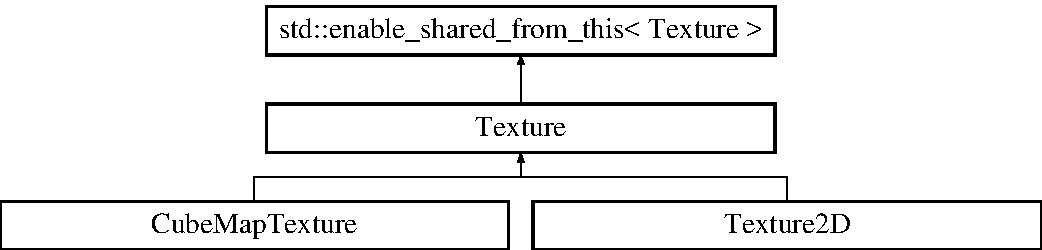
\includegraphics[height=3.000000cm]{class_texture}
\end{center}
\end{figure}
\subsection*{Public Member Functions}
\begin{DoxyCompactItemize}
\item
\hyperlink{class_texture_aa9661e01f3c034c259c15b619e2cea55}{Texture} (G\+Lenum input\+Target)
\item
virtual \hyperlink{class_texture_a09c4bcb7462f64c1d20fa69dba3cee8a}{$\sim$\+Texture} ()
\begin{DoxyCompactList}\small\item\em Destructor. \end{DoxyCompactList}\item
virtual void \hyperlink{class_texture_a6c9fda62e4203d0545ec0d3d0551760d}{Begin\+Render} (int unit) const
\begin{DoxyCompactList}\small\item\em Binds the texture to a texture unit and sets the target as G\+L\+\_\+\+T\+E\+X\+T\+U\+R\+E\+\_\+2D. \end{DoxyCompactList}\item
virtual void \hyperlink{class_texture_ab3fc771da58d58e1f3701b1fae12880b}{End\+Render} () const
\begin{DoxyCompactList}\small\item\em Unbinds the texture. \end{DoxyCompactList}\end{DoxyCompactItemize}
\subsection*{Protected Attributes}
\begin{DoxyCompactItemize}
\item
G\+Lenum \hyperlink{class_texture_a743402dc306a143404ee2d246d864fb7}{texture\+Target}
\item
G\+Luint \hyperlink{class_texture_adbf320788255a426a0a60e35cd969bcd}{gl\+Texture}
\end{DoxyCompactItemize}


\subsection{Detailed Description}
Stores the assignment framework\textquotesingle{}s representation of a texture and allows reuse of the underlying Open\+GL texture.

Note that this class does not handle loading the texture. To see how a texture is loaded, look at \hyperlink{namespace_texture_loader_aed2af32d44d07368f1f426c4274418c0}{Texture\+Loader\+::\+Load\+Texture()}.

\subsection{Constructor \& Destructor Documentation}
\hypertarget{class_texture_aa9661e01f3c034c259c15b619e2cea55}{}\label{class_texture_aa9661e01f3c034c259c15b619e2cea55}
\index{Texture@{Texture}!Texture@{Texture}}
\index{Texture@{Texture}!Texture@{Texture}}
\subsubsection{\texorpdfstring{Texture()}{Texture()}}
{\footnotesize\ttfamily Texture\+::\+Texture (\begin{DoxyParamCaption}\item[{G\+Lenum}]{input\+Target }\end{DoxyParamCaption})}

\hypertarget{class_texture_a09c4bcb7462f64c1d20fa69dba3cee8a}{}\label{class_texture_a09c4bcb7462f64c1d20fa69dba3cee8a}
\index{Texture@{Texture}!````~Texture@{$\sim$\+Texture}}
\index{````~Texture@{$\sim$\+Texture}!Texture@{Texture}}
\subsubsection{\texorpdfstring{$\sim$\+Texture()}{~Texture()}}
{\footnotesize\ttfamily Texture\+::$\sim$\+Texture (\begin{DoxyParamCaption}{ }\end{DoxyParamCaption})\hspace{0.3cm}{\ttfamily [virtual]}}



Destructor.



\subsection{Member Function Documentation}
\hypertarget{class_texture_a6c9fda62e4203d0545ec0d3d0551760d}{}\label{class_texture_a6c9fda62e4203d0545ec0d3d0551760d}
\index{Texture@{Texture}!Begin\+Render@{Begin\+Render}}
\index{Begin\+Render@{Begin\+Render}!Texture@{Texture}}
\subsubsection{\texorpdfstring{Begin\+Render()}{BeginRender()}}
{\footnotesize\ttfamily void Texture\+::\+Begin\+Render (\begin{DoxyParamCaption}\item[{int}]{unit }\end{DoxyParamCaption}) const\hspace{0.3cm}{\ttfamily [virtual]}}



Binds the texture to a texture unit and sets the target as G\+L\+\_\+\+T\+E\+X\+T\+U\+R\+E\+\_\+2D.


\begin{DoxyParams}{Parameters}
{\em unit} & The texture unit to bind to. \\
\hline
\end{DoxyParams}
\hypertarget{class_texture_ab3fc771da58d58e1f3701b1fae12880b}{}\label{class_texture_ab3fc771da58d58e1f3701b1fae12880b}
\index{Texture@{Texture}!End\+Render@{End\+Render}}
\index{End\+Render@{End\+Render}!Texture@{Texture}}
\subsubsection{\texorpdfstring{End\+Render()}{EndRender()}}
{\footnotesize\ttfamily void Texture\+::\+End\+Render (\begin{DoxyParamCaption}{ }\end{DoxyParamCaption}) const\hspace{0.3cm}{\ttfamily [virtual]}}



Unbinds the texture.



\subsection{Member Data Documentation}
\hypertarget{class_texture_adbf320788255a426a0a60e35cd969bcd}{}\label{class_texture_adbf320788255a426a0a60e35cd969bcd}
\index{Texture@{Texture}!gl\+Texture@{gl\+Texture}}
\index{gl\+Texture@{gl\+Texture}!Texture@{Texture}}
\subsubsection{\texorpdfstring{gl\+Texture}{glTexture}}
{\footnotesize\ttfamily G\+Luint Texture\+::gl\+Texture\hspace{0.3cm}{\ttfamily [protected]}}

\hypertarget{class_texture_a743402dc306a143404ee2d246d864fb7}{}\label{class_texture_a743402dc306a143404ee2d246d864fb7}
\index{Texture@{Texture}!texture\+Target@{texture\+Target}}
\index{texture\+Target@{texture\+Target}!Texture@{Texture}}
\subsubsection{\texorpdfstring{texture\+Target}{textureTarget}}
{\footnotesize\ttfamily G\+Lenum Texture\+::texture\+Target\hspace{0.3cm}{\ttfamily [protected]}}



The documentation for this class was generated from the following files\+:\begin{DoxyCompactItemize}
\item
/data/MO814A-MC937A/MO814A-MC937Aopengl-\/instructor/source/common/\+Rendering/\+Textures/\hyperlink{_texture_8h}{Texture.\+h}\item
/data/MO814A-MC937A/MO814A-MC937Aopengl-\/instructor/source/common/\+Rendering/\+Textures/\hyperlink{_texture_8cpp}{Texture.\+cpp}\end{DoxyCompactItemize}

\hypertarget{class_texture2_d}{}\section{Texture2D Class Reference}
\label{class_texture2_d}\index{Texture2D@{Texture2D}}


{\ttfamily \#include $<$Texture2\+D.\+h$>$}

Inheritance diagram for Texture2D\+:\begin{figure}[H]
\begin{center}
\leavevmode
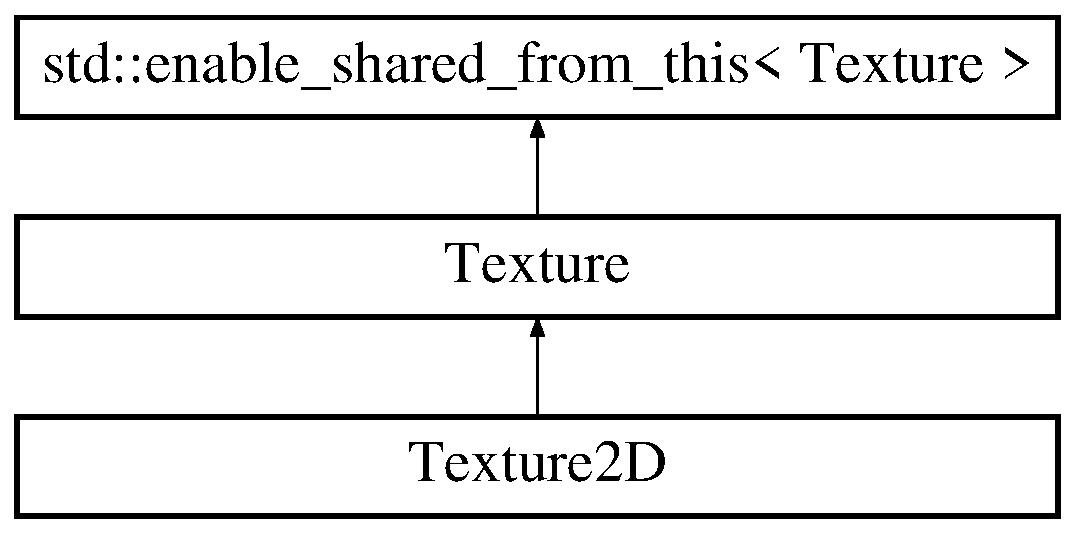
\includegraphics[height=3.000000cm]{class_texture2_d}
\end{center}
\end{figure}
\subsection*{Public Member Functions}
\begin{DoxyCompactItemize}
\item
\hyperlink{class_texture2_d_ad033510acef475ce46df4eda3d388546}{Texture2D} (G\+Lubyte $\ast$raw\+Data, int width, int height)
\begin{DoxyCompactList}\small\item\em Constructs a texture object. \end{DoxyCompactList}\end{DoxyCompactItemize}
\subsection*{Private Attributes}
\begin{DoxyCompactItemize}
\item
int \hyperlink{class_texture2_d_adf75753ea19d57141c9da0ff3298a20d}{tex\+Width}
\item
int \hyperlink{class_texture2_d_ae7a111c14c36358906cebf47e94541e2}{tex\+Height}
\end{DoxyCompactItemize}
\subsection*{Additional Inherited Members}


\subsection{Constructor \& Destructor Documentation}
\hypertarget{class_texture2_d_ad033510acef475ce46df4eda3d388546}{}\label{class_texture2_d_ad033510acef475ce46df4eda3d388546}
\index{Texture2D@{Texture2D}!Texture2D@{Texture2D}}
\index{Texture2D@{Texture2D}!Texture2D@{Texture2D}}
\subsubsection{\texorpdfstring{Texture2\+D()}{Texture2D()}}
{\footnotesize\ttfamily Texture2\+D\+::\+Texture2D (\begin{DoxyParamCaption}\item[{G\+Lubyte $\ast$}]{raw\+Data,  }\item[{int}]{width,  }\item[{int}]{height }\end{DoxyParamCaption})}



Constructs a texture object.


\begin{DoxyParams}{Parameters}
{\em raw\+Data} & The raw pointer to the pixel R\+G\+BA data. \\
\hline
{\em width} & The width of the texture. \\
\hline
{\em height} & The height of the texture.\\
\hline
\end{DoxyParams}
Takes in the raw pixel data for a texture and creates an R\+G\+BA texture out of it. Note that only R\+G\+BA textures are currently supported. Additionally, we assume the data is stored such it describes the texture from bottom to top, one row at a time (aka rows are contiguous in memory, beginning from the bottom row).

\subsection{Member Data Documentation}
\hypertarget{class_texture2_d_ae7a111c14c36358906cebf47e94541e2}{}\label{class_texture2_d_ae7a111c14c36358906cebf47e94541e2}
\index{Texture2D@{Texture2D}!tex\+Height@{tex\+Height}}
\index{tex\+Height@{tex\+Height}!Texture2D@{Texture2D}}
\subsubsection{\texorpdfstring{tex\+Height}{texHeight}}
{\footnotesize\ttfamily int Texture2\+D\+::tex\+Height\hspace{0.3cm}{\ttfamily [private]}}

\hypertarget{class_texture2_d_adf75753ea19d57141c9da0ff3298a20d}{}\label{class_texture2_d_adf75753ea19d57141c9da0ff3298a20d}
\index{Texture2D@{Texture2D}!tex\+Width@{tex\+Width}}
\index{tex\+Width@{tex\+Width}!Texture2D@{Texture2D}}
\subsubsection{\texorpdfstring{tex\+Width}{texWidth}}
{\footnotesize\ttfamily int Texture2\+D\+::tex\+Width\hspace{0.3cm}{\ttfamily [private]}}



The documentation for this class was generated from the following files\+:\begin{DoxyCompactItemize}
\item
/data/MO814A-MC937A/MO814A-MC937Aopengl-\/instructor/source/common/\+Rendering/\+Textures/\hyperlink{_texture2_d_8h}{Texture2\+D.\+h}\item
/data/MO814A-MC937A/MO814A-MC937Aopengl-\/instructor/source/common/\+Rendering/\+Textures/\hyperlink{_texture2_d_8cpp}{Texture2\+D.\+cpp}\end{DoxyCompactItemize}

\hypertarget{struct_blinn_phong_shader_1_1_texture_slots}{}\section{Blinn\+Phong\+Shader\+:\+:Texture\+Slots Struct Reference}
\label{struct_blinn_phong_shader_1_1_texture_slots}\index{Blinn\+Phong\+Shader\+::\+Texture\+Slots@{Blinn\+Phong\+Shader\+::\+Texture\+Slots}}


Corresponds to the texture unit that we want to bind the texture to.




{\ttfamily \#include $<$Blinn\+Phong\+Shader.\+h$>$}

\subsection*{Public Types}
\begin{DoxyCompactItemize}
\item
enum \hyperlink{struct_blinn_phong_shader_1_1_texture_slots_a98940b49ba855ee47d61a6243c05c34d}{Type} \{ \hyperlink{struct_blinn_phong_shader_1_1_texture_slots_a98940b49ba855ee47d61a6243c05c34da186e353d3c15d10c2020688e6d19f848}{D\+I\+F\+F\+U\+SE} = 0,
\hyperlink{struct_blinn_phong_shader_1_1_texture_slots_a98940b49ba855ee47d61a6243c05c34daecb7e8082bc31bc5bb4318591411eb70}{S\+P\+E\+C\+U\+L\+AR},
\hyperlink{struct_blinn_phong_shader_1_1_texture_slots_a98940b49ba855ee47d61a6243c05c34da9c8fe4cf162e05245c9be7b4c28cf227}{N\+O\+R\+M\+AL},
\hyperlink{struct_blinn_phong_shader_1_1_texture_slots_a98940b49ba855ee47d61a6243c05c34da7cacdf320db9a183b63d7d76dba8a4f6}{D\+I\+S\+P\+L\+A\+C\+E\+M\+E\+NT}
 \}
\end{DoxyCompactItemize}


\subsection{Detailed Description}
Corresponds to the texture unit that we want to bind the texture to.

We specify the active texture unit using \href{https://www.opengl.org/sdk/docs/man/html/glActiveTexture.xhtml}{\tt gl\+Active\+Texture}. The texture unit has a different role than the texture target (i.\+e. G\+L\+\_\+\+T\+E\+X\+T\+U\+R\+E\+\_\+2D). You can read more about it \href{https://www.opengl.org/wiki/Texture}{\tt here}.

\subsection{Member Enumeration Documentation}
\hypertarget{struct_blinn_phong_shader_1_1_texture_slots_a98940b49ba855ee47d61a6243c05c34d}{}\label{struct_blinn_phong_shader_1_1_texture_slots_a98940b49ba855ee47d61a6243c05c34d}
\index{Blinn\+Phong\+Shader\+::\+Texture\+Slots@{Blinn\+Phong\+Shader\+::\+Texture\+Slots}!Type@{Type}}
\index{Type@{Type}!Blinn\+Phong\+Shader\+::\+Texture\+Slots@{Blinn\+Phong\+Shader\+::\+Texture\+Slots}}
\subsubsection{\texorpdfstring{Type}{Type}}
{\footnotesize\ttfamily enum \hyperlink{struct_blinn_phong_shader_1_1_texture_slots_a98940b49ba855ee47d61a6243c05c34d}{Blinn\+Phong\+Shader\+::\+Texture\+Slots\+::\+Type}}

\begin{DoxyEnumFields}{Enumerator}
\raisebox{\heightof{T}}[0pt][0pt]{\index{D\+I\+F\+F\+U\+SE@{D\+I\+F\+F\+U\+SE}!Blinn\+Phong\+Shader\+::\+Texture\+Slots@{Blinn\+Phong\+Shader\+::\+Texture\+Slots}}\index{Blinn\+Phong\+Shader\+::\+Texture\+Slots@{Blinn\+Phong\+Shader\+::\+Texture\+Slots}!D\+I\+F\+F\+U\+SE@{D\+I\+F\+F\+U\+SE}}}\hypertarget{struct_blinn_phong_shader_1_1_texture_slots_a98940b49ba855ee47d61a6243c05c34da186e353d3c15d10c2020688e6d19f848}{}\label{struct_blinn_phong_shader_1_1_texture_slots_a98940b49ba855ee47d61a6243c05c34da186e353d3c15d10c2020688e6d19f848}
D\+I\+F\+F\+U\+SE&\\
\hline

\raisebox{\heightof{T}}[0pt][0pt]{\index{S\+P\+E\+C\+U\+L\+AR@{S\+P\+E\+C\+U\+L\+AR}!Blinn\+Phong\+Shader\+::\+Texture\+Slots@{Blinn\+Phong\+Shader\+::\+Texture\+Slots}}\index{Blinn\+Phong\+Shader\+::\+Texture\+Slots@{Blinn\+Phong\+Shader\+::\+Texture\+Slots}!S\+P\+E\+C\+U\+L\+AR@{S\+P\+E\+C\+U\+L\+AR}}}\hypertarget{struct_blinn_phong_shader_1_1_texture_slots_a98940b49ba855ee47d61a6243c05c34daecb7e8082bc31bc5bb4318591411eb70}{}\label{struct_blinn_phong_shader_1_1_texture_slots_a98940b49ba855ee47d61a6243c05c34daecb7e8082bc31bc5bb4318591411eb70}
S\+P\+E\+C\+U\+L\+AR&\\
\hline

\raisebox{\heightof{T}}[0pt][0pt]{\index{N\+O\+R\+M\+AL@{N\+O\+R\+M\+AL}!Blinn\+Phong\+Shader\+::\+Texture\+Slots@{Blinn\+Phong\+Shader\+::\+Texture\+Slots}}\index{Blinn\+Phong\+Shader\+::\+Texture\+Slots@{Blinn\+Phong\+Shader\+::\+Texture\+Slots}!N\+O\+R\+M\+AL@{N\+O\+R\+M\+AL}}}\hypertarget{struct_blinn_phong_shader_1_1_texture_slots_a98940b49ba855ee47d61a6243c05c34da9c8fe4cf162e05245c9be7b4c28cf227}{}\label{struct_blinn_phong_shader_1_1_texture_slots_a98940b49ba855ee47d61a6243c05c34da9c8fe4cf162e05245c9be7b4c28cf227}
N\+O\+R\+M\+AL&\\
\hline

\raisebox{\heightof{T}}[0pt][0pt]{\index{D\+I\+S\+P\+L\+A\+C\+E\+M\+E\+NT@{D\+I\+S\+P\+L\+A\+C\+E\+M\+E\+NT}!Blinn\+Phong\+Shader\+::\+Texture\+Slots@{Blinn\+Phong\+Shader\+::\+Texture\+Slots}}\index{Blinn\+Phong\+Shader\+::\+Texture\+Slots@{Blinn\+Phong\+Shader\+::\+Texture\+Slots}!D\+I\+S\+P\+L\+A\+C\+E\+M\+E\+NT@{D\+I\+S\+P\+L\+A\+C\+E\+M\+E\+NT}}}\hypertarget{struct_blinn_phong_shader_1_1_texture_slots_a98940b49ba855ee47d61a6243c05c34da7cacdf320db9a183b63d7d76dba8a4f6}{}\label{struct_blinn_phong_shader_1_1_texture_slots_a98940b49ba855ee47d61a6243c05c34da7cacdf320db9a183b63d7d76dba8a4f6}
D\+I\+S\+P\+L\+A\+C\+E\+M\+E\+NT&\\
\hline

\end{DoxyEnumFields}


The documentation for this struct was generated from the following file\+:\begin{DoxyCompactItemize}
\item
/data/MO814A-MC937A/MO814A-MC937Aopengl-\/instructor/source/common/\+Rendering/\+Shaders/\hyperlink{_blinn_phong_shader_8h}{Blinn\+Phong\+Shader.\+h}\end{DoxyCompactItemize}

\chapter{File Documentation}
\hypertarget{_assignment1_8cpp}{}\section{/data/MO814A-MC937A/MO814A-MC937Aopengl-\/instructor/source/assignment1/\+Assignment1.cpp File Reference}
\label{_assignment1_8cpp}\index{/data/MO814A-MC937A/MO814A-MC937Aopengl-\/instructor/source/assignment1/\+Assignment1.\+cpp@{/data/MO814A-MC937A/MO814A-MC937Aopengl-\/instructor/source/assignment1/\+Assignment1.\+cpp}}
{\ttfamily \#include \char`\"{}assignment1/\+Assignment1.\+h\char`\"{}}\newline
{\ttfamily \#include \char`\"{}common/core.\+h\char`\"{}}\newline

\hypertarget{_assignment1_8h}{}\section{/data/MO814A-MC937A/MO814A-MC937Aopengl-\/instructor/source/assignment1/\+Assignment1.h File Reference}
\label{_assignment1_8h}\index{/data/MO814A-MC937A/MO814A-MC937Aopengl-\/instructor/source/assignment1/\+Assignment1.\+h@{/data/MO814A-MC937A/MO814A-MC937Aopengl-\/instructor/source/assignment1/\+Assignment1.\+h}}
{\ttfamily \#include \char`\"{}common/\+Application.\+h\char`\"{}}\newline
\subsection*{Classes}
\begin{DoxyCompactItemize}
\item
class \hyperlink{class_assignment1}{Assignment1}
\end{DoxyCompactItemize}
\subsection*{Macros}
\begin{DoxyCompactItemize}
\item
\#define \hyperlink{_assignment1_8h_ab35701035e592ccaccd4686be0e98905}{\+\_\+\+\_\+\+A\+S\+S\+I\+G\+N\+M\+E\+N\+T\+\_\+1\+\_\+\+\_\+}
\end{DoxyCompactItemize}


\subsection{Macro Definition Documentation}
\hypertarget{_assignment1_8h_ab35701035e592ccaccd4686be0e98905}{}\label{_assignment1_8h_ab35701035e592ccaccd4686be0e98905}
\index{Assignment1.\+h@{Assignment1.\+h}!\+\_\+\+\_\+\+A\+S\+S\+I\+G\+N\+M\+E\+N\+T\+\_\+1\+\_\+\+\_\+@{\+\_\+\+\_\+\+A\+S\+S\+I\+G\+N\+M\+E\+N\+T\+\_\+1\+\_\+\+\_\+}}
\index{\+\_\+\+\_\+\+A\+S\+S\+I\+G\+N\+M\+E\+N\+T\+\_\+1\+\_\+\+\_\+@{\+\_\+\+\_\+\+A\+S\+S\+I\+G\+N\+M\+E\+N\+T\+\_\+1\+\_\+\+\_\+}!Assignment1.\+h@{Assignment1.\+h}}
\subsubsection{\texorpdfstring{\+\_\+\+\_\+\+A\+S\+S\+I\+G\+N\+M\+E\+N\+T\+\_\+1\+\_\+\+\_\+}{\_\_ASSIGNMENT\_1\_\_}}
{\footnotesize\ttfamily \#define \+\_\+\+\_\+\+A\+S\+S\+I\+G\+N\+M\+E\+N\+T\+\_\+1\+\_\+\+\_\+}

\hypertarget{_assignment2_8cpp}{}\section{/data/MO814A-MC937A/MO814A-MC937Aopengl-\/instructor/source/assignment2/\+Assignment2.cpp File Reference}
\label{_assignment2_8cpp}\index{/data/MO814A-MC937A/MO814A-MC937Aopengl-\/instructor/source/assignment2/\+Assignment2.\+cpp@{/data/MO814A-MC937A/MO814A-MC937Aopengl-\/instructor/source/assignment2/\+Assignment2.\+cpp}}
{\ttfamily \#include \char`\"{}assignment2/\+Assignment2.\+h\char`\"{}}\newline
{\ttfamily \#include \char`\"{}common/core.\+h\char`\"{}}\newline
{\ttfamily \#include \char`\"{}common/\+Utility/\+Mesh/\+Simple/\+Primitive\+Creator.\+h\char`\"{}}\newline
{\ttfamily \#include \char`\"{}common/\+Utility/\+Mesh/\+Loading/\+Mesh\+Loader.\+h\char`\"{}}\newline
{\ttfamily \#include $<$cmath$>$}\newline

\hypertarget{_assignment2_8h}{}\section{/data/MO814A-MC937A/MO814A-MC937Aopengl-\/instructor/source/assignment2/\+Assignment2.h File Reference}
\label{_assignment2_8h}\index{/data/MO814A-MC937A/MO814A-MC937Aopengl-\/instructor/source/assignment2/\+Assignment2.\+h@{/data/MO814A-MC937A/MO814A-MC937Aopengl-\/instructor/source/assignment2/\+Assignment2.\+h}}
{\ttfamily \#include \char`\"{}common/\+Application.\+h\char`\"{}}\newline
\subsection*{Classes}
\begin{DoxyCompactItemize}
\item
class \hyperlink{class_assignment2}{Assignment2}
\end{DoxyCompactItemize}
\subsection*{Macros}
\begin{DoxyCompactItemize}
\item
\#define \hyperlink{_assignment2_8h_a2e5bb565ef0b47ac4e4ba4d83cb2ab4d}{\+\_\+\+\_\+\+A\+S\+S\+I\+G\+N\+M\+E\+N\+T\+\_\+2\+\_\+\+\_\+}
\end{DoxyCompactItemize}


\subsection{Macro Definition Documentation}
\hypertarget{_assignment2_8h_a2e5bb565ef0b47ac4e4ba4d83cb2ab4d}{}\label{_assignment2_8h_a2e5bb565ef0b47ac4e4ba4d83cb2ab4d}
\index{Assignment2.\+h@{Assignment2.\+h}!\+\_\+\+\_\+\+A\+S\+S\+I\+G\+N\+M\+E\+N\+T\+\_\+2\+\_\+\+\_\+@{\+\_\+\+\_\+\+A\+S\+S\+I\+G\+N\+M\+E\+N\+T\+\_\+2\+\_\+\+\_\+}}
\index{\+\_\+\+\_\+\+A\+S\+S\+I\+G\+N\+M\+E\+N\+T\+\_\+2\+\_\+\+\_\+@{\+\_\+\+\_\+\+A\+S\+S\+I\+G\+N\+M\+E\+N\+T\+\_\+2\+\_\+\+\_\+}!Assignment2.\+h@{Assignment2.\+h}}
\subsubsection{\texorpdfstring{\+\_\+\+\_\+\+A\+S\+S\+I\+G\+N\+M\+E\+N\+T\+\_\+2\+\_\+\+\_\+}{\_\_ASSIGNMENT\_2\_\_}}
{\footnotesize\ttfamily \#define \+\_\+\+\_\+\+A\+S\+S\+I\+G\+N\+M\+E\+N\+T\+\_\+2\+\_\+\+\_\+}

\hypertarget{_assignment3_8cpp}{}\section{/data/MO814A-MC937A/MO814A-MC937Aopengl-\/instructor/source/assignment3/\+Assignment3.cpp File Reference}
\label{_assignment3_8cpp}\index{/data/MO814A-MC937A/MO814A-MC937Aopengl-\/instructor/source/assignment3/\+Assignment3.\+cpp@{/data/MO814A-MC937A/MO814A-MC937Aopengl-\/instructor/source/assignment3/\+Assignment3.\+cpp}}
{\ttfamily \#include \char`\"{}assignment3/\+Assignment3.\+h\char`\"{}}\newline
{\ttfamily \#include \char`\"{}common/core.\+h\char`\"{}}\newline
{\ttfamily \#include \char`\"{}common/\+Utility/\+Mesh/\+Simple/\+Primitive\+Creator.\+h\char`\"{}}\newline
{\ttfamily \#include \char`\"{}common/\+Utility/\+Mesh/\+Loading/\+Mesh\+Loader.\+h\char`\"{}}\newline
{\ttfamily \#include $<$cmath$>$}\newline

\hypertarget{_assignment3_8h}{}\section{/data/MO814A-MC937A/MO814A-MC937Aopengl-\/instructor/source/assignment3/\+Assignment3.h File Reference}
\label{_assignment3_8h}\index{/data/MO814A-MC937A/MO814A-MC937Aopengl-\/instructor/source/assignment3/\+Assignment3.\+h@{/data/MO814A-MC937A/MO814A-MC937Aopengl-\/instructor/source/assignment3/\+Assignment3.\+h}}
{\ttfamily \#include \char`\"{}common/\+Application.\+h\char`\"{}}\newline
\subsection*{Classes}
\begin{DoxyCompactItemize}
\item
class \hyperlink{class_assignment3}{Assignment3}
\end{DoxyCompactItemize}
\subsection*{Macros}
\begin{DoxyCompactItemize}
\item
\#define \hyperlink{_assignment3_8h_aad53bf863e2c49f7131e6c381f6177bb}{\+\_\+\+\_\+\+A\+S\+S\+I\+G\+N\+M\+E\+N\+T\+\_\+3\+\_\+\+\_\+}
\end{DoxyCompactItemize}


\subsection{Macro Definition Documentation}
\hypertarget{_assignment3_8h_aad53bf863e2c49f7131e6c381f6177bb}{}\label{_assignment3_8h_aad53bf863e2c49f7131e6c381f6177bb}
\index{Assignment3.\+h@{Assignment3.\+h}!\+\_\+\+\_\+\+A\+S\+S\+I\+G\+N\+M\+E\+N\+T\+\_\+3\+\_\+\+\_\+@{\+\_\+\+\_\+\+A\+S\+S\+I\+G\+N\+M\+E\+N\+T\+\_\+3\+\_\+\+\_\+}}
\index{\+\_\+\+\_\+\+A\+S\+S\+I\+G\+N\+M\+E\+N\+T\+\_\+3\+\_\+\+\_\+@{\+\_\+\+\_\+\+A\+S\+S\+I\+G\+N\+M\+E\+N\+T\+\_\+3\+\_\+\+\_\+}!Assignment3.\+h@{Assignment3.\+h}}
\subsubsection{\texorpdfstring{\+\_\+\+\_\+\+A\+S\+S\+I\+G\+N\+M\+E\+N\+T\+\_\+3\+\_\+\+\_\+}{\_\_ASSIGNMENT\_3\_\_}}
{\footnotesize\ttfamily \#define \+\_\+\+\_\+\+A\+S\+S\+I\+G\+N\+M\+E\+N\+T\+\_\+3\+\_\+\+\_\+}

\hypertarget{_assignment4_8cpp}{}\section{/data/MO814A-MC937A/MO814A-MC937Aopengl-\/instructor/source/assignment4/\+Assignment4.cpp File Reference}
\label{_assignment4_8cpp}\index{/data/MO814A-MC937A/MO814A-MC937Aopengl-\/instructor/source/assignment4/\+Assignment4.\+cpp@{/data/MO814A-MC937A/MO814A-MC937Aopengl-\/instructor/source/assignment4/\+Assignment4.\+cpp}}
{\ttfamily \#include \char`\"{}assignment4/\+Assignment4.\+h\char`\"{}}\newline
{\ttfamily \#include \char`\"{}common/core.\+h\char`\"{}}\newline
{\ttfamily \#include \char`\"{}common/\+Utility/\+Mesh/\+Simple/\+Primitive\+Creator.\+h\char`\"{}}\newline
{\ttfamily \#include \char`\"{}common/\+Utility/\+Mesh/\+Loading/\+Mesh\+Loader.\+h\char`\"{}}\newline
{\ttfamily \#include \char`\"{}common/\+Utility/\+Texture/\+Texture\+Loader.\+h\char`\"{}}\newline
{\ttfamily \#include $<$cmath$>$}\newline

\hypertarget{_assignment4_8h}{}\section{/data/MO814A-MC937A/MO814A-MC937Aopengl-\/instructor/source/assignment4/\+Assignment4.h File Reference}
\label{_assignment4_8h}\index{/data/MO814A-MC937A/MO814A-MC937Aopengl-\/instructor/source/assignment4/\+Assignment4.\+h@{/data/MO814A-MC937A/MO814A-MC937Aopengl-\/instructor/source/assignment4/\+Assignment4.\+h}}
{\ttfamily \#include \char`\"{}common/\+Application.\+h\char`\"{}}\newline
\subsection*{Classes}
\begin{DoxyCompactItemize}
\item
class \hyperlink{class_assignment4}{Assignment4}
\end{DoxyCompactItemize}
\subsection*{Macros}
\begin{DoxyCompactItemize}
\item
\#define \hyperlink{_assignment4_8h_a9c91d60c420111fc7900d211f4b5a197}{\+\_\+\+\_\+\+A\+S\+S\+I\+G\+N\+M\+E\+N\+T\+\_\+4\+\_\+\+\_\+}
\end{DoxyCompactItemize}


\subsection{Macro Definition Documentation}
\hypertarget{_assignment4_8h_a9c91d60c420111fc7900d211f4b5a197}{}\label{_assignment4_8h_a9c91d60c420111fc7900d211f4b5a197}
\index{Assignment4.\+h@{Assignment4.\+h}!\+\_\+\+\_\+\+A\+S\+S\+I\+G\+N\+M\+E\+N\+T\+\_\+4\+\_\+\+\_\+@{\+\_\+\+\_\+\+A\+S\+S\+I\+G\+N\+M\+E\+N\+T\+\_\+4\+\_\+\+\_\+}}
\index{\+\_\+\+\_\+\+A\+S\+S\+I\+G\+N\+M\+E\+N\+T\+\_\+4\+\_\+\+\_\+@{\+\_\+\+\_\+\+A\+S\+S\+I\+G\+N\+M\+E\+N\+T\+\_\+4\+\_\+\+\_\+}!Assignment4.\+h@{Assignment4.\+h}}
\subsubsection{\texorpdfstring{\+\_\+\+\_\+\+A\+S\+S\+I\+G\+N\+M\+E\+N\+T\+\_\+4\+\_\+\+\_\+}{\_\_ASSIGNMENT\_4\_\_}}
{\footnotesize\ttfamily \#define \+\_\+\+\_\+\+A\+S\+S\+I\+G\+N\+M\+E\+N\+T\+\_\+4\+\_\+\+\_\+}

\hypertarget{_assignment5_8cpp}{}\section{/data/MO814A-MC937A/MO814A-MC937Aopengl-\/instructor/source/assignment5/\+Assignment5.cpp File Reference}
\label{_assignment5_8cpp}\index{/data/MO814A-MC937A/MO814A-MC937Aopengl-\/instructor/source/assignment5/\+Assignment5.\+cpp@{/data/MO814A-MC937A/MO814A-MC937Aopengl-\/instructor/source/assignment5/\+Assignment5.\+cpp}}
{\ttfamily \#include \char`\"{}assignment5/\+Assignment5.\+h\char`\"{}}\newline
{\ttfamily \#include \char`\"{}common/core.\+h\char`\"{}}\newline
{\ttfamily \#include \char`\"{}common/\+Utility/\+Mesh/\+Simple/\+Primitive\+Creator.\+h\char`\"{}}\newline
{\ttfamily \#include \char`\"{}common/\+Utility/\+Mesh/\+Loading/\+Mesh\+Loader.\+h\char`\"{}}\newline
{\ttfamily \#include \char`\"{}common/\+Utility/\+Texture/\+Texture\+Loader.\+h\char`\"{}}\newline

\hypertarget{_assignment5_8h}{}\section{/data/MO814A-MC937A/MO814A-MC937Aopengl-\/instructor/source/assignment5/\+Assignment5.h File Reference}
\label{_assignment5_8h}\index{/data/MO814A-MC937A/MO814A-MC937Aopengl-\/instructor/source/assignment5/\+Assignment5.\+h@{/data/MO814A-MC937A/MO814A-MC937Aopengl-\/instructor/source/assignment5/\+Assignment5.\+h}}
{\ttfamily \#include \char`\"{}common/\+Application.\+h\char`\"{}}\newline
\subsection*{Classes}
\begin{DoxyCompactItemize}
\item
class \hyperlink{class_assignment5}{Assignment5}
\end{DoxyCompactItemize}
\subsection*{Macros}
\begin{DoxyCompactItemize}
\item
\#define \hyperlink{_assignment5_8h_a37a7ba6eb0864f764e3a19e1f964efef}{\+\_\+\+\_\+\+A\+S\+S\+I\+G\+N\+M\+E\+N\+T\+\_\+5\+\_\+\+\_\+}
\end{DoxyCompactItemize}


\subsection{Macro Definition Documentation}
\hypertarget{_assignment5_8h_a37a7ba6eb0864f764e3a19e1f964efef}{}\label{_assignment5_8h_a37a7ba6eb0864f764e3a19e1f964efef}
\index{Assignment5.\+h@{Assignment5.\+h}!\+\_\+\+\_\+\+A\+S\+S\+I\+G\+N\+M\+E\+N\+T\+\_\+5\+\_\+\+\_\+@{\+\_\+\+\_\+\+A\+S\+S\+I\+G\+N\+M\+E\+N\+T\+\_\+5\+\_\+\+\_\+}}
\index{\+\_\+\+\_\+\+A\+S\+S\+I\+G\+N\+M\+E\+N\+T\+\_\+5\+\_\+\+\_\+@{\+\_\+\+\_\+\+A\+S\+S\+I\+G\+N\+M\+E\+N\+T\+\_\+5\+\_\+\+\_\+}!Assignment5.\+h@{Assignment5.\+h}}
\subsubsection{\texorpdfstring{\+\_\+\+\_\+\+A\+S\+S\+I\+G\+N\+M\+E\+N\+T\+\_\+5\+\_\+\+\_\+}{\_\_ASSIGNMENT\_5\_\_}}
{\footnotesize\ttfamily \#define \+\_\+\+\_\+\+A\+S\+S\+I\+G\+N\+M\+E\+N\+T\+\_\+5\+\_\+\+\_\+}

\hypertarget{_application_8cpp}{}\section{/data/MO814A-MC937A/MO814A-MC937Aopengl-\/instructor/source/common/\+Application.cpp File Reference}
\label{_application_8cpp}\index{/data/MO814A-MC937A/MO814A-MC937Aopengl-\/instructor/source/common/\+Application.\+cpp@{/data/MO814A-MC937A/MO814A-MC937Aopengl-\/instructor/source/common/\+Application.\+cpp}}
{\ttfamily \#include \char`\"{}common/\+Application.\+h\char`\"{}}\newline
{\ttfamily \#include \char`\"{}common/\+Rendering/\+Forward\+Renderer.\+h\char`\"{}}\newline
{\ttfamily \#include \char`\"{}common/\+Scene/\+Scene.\+h\char`\"{}}\newline
{\ttfamily \#include \char`\"{}common/\+Scene/\+Camera/\+Camera.\+h\char`\"{}}\newline

\hypertarget{_application_8h}{}\section{/data/MO814A-MC937A/MO814A-MC937Aopengl-\/instructor/source/common/\+Application.h File Reference}
\label{_application_8h}\index{/data/MO814A-MC937A/MO814A-MC937Aopengl-\/instructor/source/common/\+Application.\+h@{/data/MO814A-MC937A/MO814A-MC937Aopengl-\/instructor/source/common/\+Application.\+h}}
{\ttfamily \#include \char`\"{}common/common.\+h\char`\"{}}\newline
\subsection*{Classes}
\begin{DoxyCompactItemize}
\item
class \hyperlink{class_application}{Application}
\begin{DoxyCompactList}\small\item\em Handles creating configurable objects (i.\+e. scene, camera, renderer), handling S\+DL events passed in by the \hyperlink{class_media_layer}{Media\+Layer}, and handles creating the scene to be display. \end{DoxyCompactList}\end{DoxyCompactItemize}
\subsection*{Macros}
\begin{DoxyCompactItemize}
\item
\#define \hyperlink{_application_8h_a1034695410f242c9eb3c1a58c61e9bd7}{\+\_\+\+\_\+\+A\+P\+P\+L\+I\+C\+A\+T\+I\+O\+N\+\_\+\+\_\+}
\end{DoxyCompactItemize}


\subsection{Macro Definition Documentation}
\hypertarget{_application_8h_a1034695410f242c9eb3c1a58c61e9bd7}{}\label{_application_8h_a1034695410f242c9eb3c1a58c61e9bd7}
\index{Application.\+h@{Application.\+h}!\+\_\+\+\_\+\+A\+P\+P\+L\+I\+C\+A\+T\+I\+O\+N\+\_\+\+\_\+@{\+\_\+\+\_\+\+A\+P\+P\+L\+I\+C\+A\+T\+I\+O\+N\+\_\+\+\_\+}}
\index{\+\_\+\+\_\+\+A\+P\+P\+L\+I\+C\+A\+T\+I\+O\+N\+\_\+\+\_\+@{\+\_\+\+\_\+\+A\+P\+P\+L\+I\+C\+A\+T\+I\+O\+N\+\_\+\+\_\+}!Application.\+h@{Application.\+h}}
\subsubsection{\texorpdfstring{\+\_\+\+\_\+\+A\+P\+P\+L\+I\+C\+A\+T\+I\+O\+N\+\_\+\+\_\+}{\_\_APPLICATION\_\_}}
{\footnotesize\ttfamily \#define \+\_\+\+\_\+\+A\+P\+P\+L\+I\+C\+A\+T\+I\+O\+N\+\_\+\+\_\+}

\hypertarget{common_8h}{}\section{/data/MO814A-MC937A/MO814A-MC937Aopengl-\/instructor/source/common/common.h File Reference}
\label{common_8h}\index{/data/MO814A-MC937A/MO814A-MC937Aopengl-\/instructor/source/common/common.\+h@{/data/MO814A-MC937A/MO814A-MC937Aopengl-\/instructor/source/common/common.\+h}}


A file included across the application framework to include common header files and other useful functions and macros.


{\ttfamily \#include \char`\"{}S\+D\+L2/\+S\+D\+L.\+h\char`\"{}}\newline
{\ttfamily \#include \char`\"{}glm/glm.\+hpp\char`\"{}}\newline
{\ttfamily \#include \char`\"{}glm/gtc/type\+\_\+ptr.\+hpp\char`\"{}}\newline
{\ttfamily \#include \char`\"{}glm/gtc/matrix\+\_\+transform.\+hpp\char`\"{}}\newline
{\ttfamily \#include \char`\"{}glm/gtc/quaternion.\+hpp\char`\"{}}\newline
{\ttfamily \#include \char`\"{}glm/gtx/quaternion.\+hpp\char`\"{}}\newline
{\ttfamily \#include \char`\"{}glm/gtx/string\+\_\+cast.\+hpp\char`\"{}}\newline
{\ttfamily \#include \char`\"{}G\+L/glew.\+h\char`\"{}}\newline
{\ttfamily \#include $<$iostream$>$}\newline
{\ttfamily \#include $<$array$>$}\newline
{\ttfamily \#include $<$memory$>$}\newline
{\ttfamily \#include $<$vector$>$}\newline
{\ttfamily \#include $<$cassert$>$}\newline
{\ttfamily \#include $<$unordered\+\_\+map$>$}\newline
\subsection*{Macros}
\begin{DoxyCompactItemize}
\item
\#define \hyperlink{common_8h_a9cb4033779c9173d55704ed4692db3e2}{\+\_\+\+\_\+\+C\+O\+M\+M\+O\+N\+\_\+\+\_\+}
\item
\#define \hyperlink{common_8h_ab76e9d812060d1ba7e166d5b3e75355b}{O\+G\+L\+\_\+\+C\+A\+LL}(x)~x; \hyperlink{common_8h_ab11db0eff470ddd4d5f1e0dfc3786dd3}{\+\_\+\+Display\+Open\+G\+L\+Error}(\#x, \+\_\+\+\_\+\+F\+I\+L\+E\+\_\+\+\_\+, \+\_\+\+\_\+\+L\+I\+N\+E\+\_\+\+\_\+);
\begin{DoxyCompactList}\small\item\em Provides an easy to use macro that wraps around Open\+GL calls and checks their error. \end{DoxyCompactList}\item
\#define \hyperlink{common_8h_a2d743b5950d82c9ca4071ca3217a8315}{S\+T\+R\+I\+N\+G\+I\+F\+Y\+\_\+\+H\+E\+L\+P\+ER}(x)~\#x
\begin{DoxyCompactList}\small\item\em Help stringify a macro. \end{DoxyCompactList}\item
\#define \hyperlink{common_8h_a6df1d22fb5f09eccc23b9f399670cfd7}{S\+T\+R\+I\+N\+G\+I\+FY}(x)~\hyperlink{common_8h_a2d743b5950d82c9ca4071ca3217a8315}{S\+T\+R\+I\+N\+G\+I\+F\+Y\+\_\+\+H\+E\+L\+P\+ER}(x)
\begin{DoxyCompactList}\small\item\em Stringify a macro. \end{DoxyCompactList}\end{DoxyCompactItemize}
\subsection*{Functions}
\begin{DoxyCompactItemize}
\item
std\+::string \hyperlink{common_8h_afce9600873f5e1c38abefadd838fbed3}{\+\_\+\+Open\+G\+L\+Error\+To\+String} (G\+Lenum err)
\begin{DoxyCompactList}\small\item\em Converts an Open\+GL error to an std\+::string. \end{DoxyCompactList}\item
void \hyperlink{common_8h_ab11db0eff470ddd4d5f1e0dfc3786dd3}{\+\_\+\+Display\+Open\+G\+L\+Error} (std\+::string command, std\+::string file, int line)
\begin{DoxyCompactList}\small\item\em Prints a user friendly message for the most recent Open\+GL error (if any) to stdout. \end{DoxyCompactList}\item
{\footnotesize template$<$typename T , typename... Ts$>$ }\\std\+::unique\+\_\+ptr$<$ T $>$ \hyperlink{common_8h_aeaa9025fc7af5678d1211ca828c19fbf}{make\+\_\+unique} (Ts \&\&... params)
\begin{DoxyCompactList}\small\item\em Create a std\+::unique\+\_\+ptr much like std\+::make\+\_\+shared. \end{DoxyCompactList}\end{DoxyCompactItemize}
\subsection*{Variables}
\begin{DoxyCompactItemize}
\item
const float \hyperlink{common_8h_a6a1e5c0227931d99b703e1fd3adebf52}{PI} = 3.\+14159265359f
\begin{DoxyCompactList}\small\item\em The PI constant. \end{DoxyCompactList}\end{DoxyCompactItemize}


\subsection{Detailed Description}
A file included across the application framework to include common header files and other useful functions and macros.



\subsection{Macro Definition Documentation}
\hypertarget{common_8h_a9cb4033779c9173d55704ed4692db3e2}{}\label{common_8h_a9cb4033779c9173d55704ed4692db3e2}
\index{common.\+h@{common.\+h}!\+\_\+\+\_\+\+C\+O\+M\+M\+O\+N\+\_\+\+\_\+@{\+\_\+\+\_\+\+C\+O\+M\+M\+O\+N\+\_\+\+\_\+}}
\index{\+\_\+\+\_\+\+C\+O\+M\+M\+O\+N\+\_\+\+\_\+@{\+\_\+\+\_\+\+C\+O\+M\+M\+O\+N\+\_\+\+\_\+}!common.\+h@{common.\+h}}
\subsubsection{\texorpdfstring{\+\_\+\+\_\+\+C\+O\+M\+M\+O\+N\+\_\+\+\_\+}{\_\_COMMON\_\_}}
{\footnotesize\ttfamily \#define \+\_\+\+\_\+\+C\+O\+M\+M\+O\+N\+\_\+\+\_\+}

\hypertarget{common_8h_ab76e9d812060d1ba7e166d5b3e75355b}{}\label{common_8h_ab76e9d812060d1ba7e166d5b3e75355b}
\index{common.\+h@{common.\+h}!O\+G\+L\+\_\+\+C\+A\+LL@{O\+G\+L\+\_\+\+C\+A\+LL}}
\index{O\+G\+L\+\_\+\+C\+A\+LL@{O\+G\+L\+\_\+\+C\+A\+LL}!common.\+h@{common.\+h}}
\subsubsection{\texorpdfstring{O\+G\+L\+\_\+\+C\+A\+LL}{OGL\_CALL}}
{\footnotesize\ttfamily \#define O\+G\+L\+\_\+\+C\+A\+LL(\begin{DoxyParamCaption}\item[{}]{x }\end{DoxyParamCaption})~x; \hyperlink{common_8h_ab11db0eff470ddd4d5f1e0dfc3786dd3}{\+\_\+\+Display\+Open\+G\+L\+Error}(\#x, \+\_\+\+\_\+\+F\+I\+L\+E\+\_\+\+\_\+, \+\_\+\+\_\+\+L\+I\+N\+E\+\_\+\+\_\+);}



Provides an easy to use macro that wraps around Open\+GL calls and checks their error.


\begin{DoxyParams}{Parameters}
{\em x} & The Open\+GL command.\\
\hline
\end{DoxyParams}
This is only defined in the Debug build when N\+D\+E\+B\+UG is N\+OT defined. If you are unfamiliar with C++ preprocess macros, the {\bfseries F\+I\+LE} macro, or the {\bfseries L\+I\+NE} macro, you can read \href{http://www.cplusplus.com/doc/tutorial/preprocessor/}{\tt this} for more information. \hypertarget{common_8h_a6df1d22fb5f09eccc23b9f399670cfd7}{}\label{common_8h_a6df1d22fb5f09eccc23b9f399670cfd7}
\index{common.\+h@{common.\+h}!S\+T\+R\+I\+N\+G\+I\+FY@{S\+T\+R\+I\+N\+G\+I\+FY}}
\index{S\+T\+R\+I\+N\+G\+I\+FY@{S\+T\+R\+I\+N\+G\+I\+FY}!common.\+h@{common.\+h}}
\subsubsection{\texorpdfstring{S\+T\+R\+I\+N\+G\+I\+FY}{STRINGIFY}}
{\footnotesize\ttfamily \#define S\+T\+R\+I\+N\+G\+I\+FY(\begin{DoxyParamCaption}\item[{}]{x }\end{DoxyParamCaption})~\hyperlink{common_8h_a2d743b5950d82c9ca4071ca3217a8315}{S\+T\+R\+I\+N\+G\+I\+F\+Y\+\_\+\+H\+E\+L\+P\+ER}(x)}



Stringify a macro.

This takes in a macro that was defined to be a string and actually converts it into a string that can be used by the application. See \hyperlink{namespace_mesh_loader_aee3ffe862d7bf408495c62614118fd2a}{Mesh\+Loader\+::\+Load\+Mesh} for an example. Why is this nested macro necessary? You can read about it here\+: \href{https://gcc.gnu.org/onlinedocs/cpp/Stringification.html}{\tt link}. \hypertarget{common_8h_a2d743b5950d82c9ca4071ca3217a8315}{}\label{common_8h_a2d743b5950d82c9ca4071ca3217a8315}
\index{common.\+h@{common.\+h}!S\+T\+R\+I\+N\+G\+I\+F\+Y\+\_\+\+H\+E\+L\+P\+ER@{S\+T\+R\+I\+N\+G\+I\+F\+Y\+\_\+\+H\+E\+L\+P\+ER}}
\index{S\+T\+R\+I\+N\+G\+I\+F\+Y\+\_\+\+H\+E\+L\+P\+ER@{S\+T\+R\+I\+N\+G\+I\+F\+Y\+\_\+\+H\+E\+L\+P\+ER}!common.\+h@{common.\+h}}
\subsubsection{\texorpdfstring{S\+T\+R\+I\+N\+G\+I\+F\+Y\+\_\+\+H\+E\+L\+P\+ER}{STRINGIFY\_HELPER}}
{\footnotesize\ttfamily \#define S\+T\+R\+I\+N\+G\+I\+F\+Y\+\_\+\+H\+E\+L\+P\+ER(\begin{DoxyParamCaption}\item[{}]{x }\end{DoxyParamCaption})~\#x}



Help stringify a macro.



\subsection{Function Documentation}
\hypertarget{common_8h_ab11db0eff470ddd4d5f1e0dfc3786dd3}{}\label{common_8h_ab11db0eff470ddd4d5f1e0dfc3786dd3}
\index{common.\+h@{common.\+h}!\+\_\+\+Display\+Open\+G\+L\+Error@{\+\_\+\+Display\+Open\+G\+L\+Error}}
\index{\+\_\+\+Display\+Open\+G\+L\+Error@{\+\_\+\+Display\+Open\+G\+L\+Error}!common.\+h@{common.\+h}}
\subsubsection{\texorpdfstring{\+\_\+\+Display\+Open\+G\+L\+Error()}{\_DisplayOpenGLError()}}
{\footnotesize\ttfamily void \+\_\+\+Display\+Open\+G\+L\+Error (\begin{DoxyParamCaption}\item[{std\+::string}]{command,  }\item[{std\+::string}]{file,  }\item[{int}]{line }\end{DoxyParamCaption})\hspace{0.3cm}{\ttfamily [inline]}}



Prints a user friendly message for the most recent Open\+GL error (if any) to stdout.

\+\_\+\+Display\+Open\+G\+L\+Error
\begin{DoxyParams}{Parameters}
{\em command} & The command that was run. \\
\hline
{\em file} & The file from which the command was run. \\
\hline
{\em line} & The line in the file where the command was fun.\\
\hline
\end{DoxyParams}
This function is used by the O\+G\+L\+\_\+\+C\+A\+LL macro to provide debugging information in stdout when an Open\+GL A\+PI call fails. \hypertarget{common_8h_afce9600873f5e1c38abefadd838fbed3}{}\label{common_8h_afce9600873f5e1c38abefadd838fbed3}
\index{common.\+h@{common.\+h}!\+\_\+\+Open\+G\+L\+Error\+To\+String@{\+\_\+\+Open\+G\+L\+Error\+To\+String}}
\index{\+\_\+\+Open\+G\+L\+Error\+To\+String@{\+\_\+\+Open\+G\+L\+Error\+To\+String}!common.\+h@{common.\+h}}
\subsubsection{\texorpdfstring{\+\_\+\+Open\+G\+L\+Error\+To\+String()}{\_OpenGLErrorToString()}}
{\footnotesize\ttfamily std\+::string \+\_\+\+Open\+G\+L\+Error\+To\+String (\begin{DoxyParamCaption}\item[{G\+Lenum}]{err }\end{DoxyParamCaption})\hspace{0.3cm}{\ttfamily [inline]}}



Converts an Open\+GL error to an std\+::string.

\+\_\+\+Open\+G\+L\+Error\+To\+String
\begin{DoxyParams}{Parameters}
{\em err} & The Open\+GL error returned by \href{https://www.opengl.org/sdk/docs/man/html/glGetError.xhtml}{\tt gl\+Get\+Error}. \\
\hline
\end{DoxyParams}
\begin{DoxyReturn}{Returns}
A string that explain the Open\+GL error. These are copied directly from the Open\+GL documentation.
\end{DoxyReturn}
This function is called by \+\_\+\+Display\+Open\+G\+L\+Error to get a user-\/friendly message in addition to an errror code. \hypertarget{common_8h_aeaa9025fc7af5678d1211ca828c19fbf}{}\label{common_8h_aeaa9025fc7af5678d1211ca828c19fbf}
\index{common.\+h@{common.\+h}!make\+\_\+unique@{make\+\_\+unique}}
\index{make\+\_\+unique@{make\+\_\+unique}!common.\+h@{common.\+h}}
\subsubsection{\texorpdfstring{make\+\_\+unique()}{make\_unique()}}
{\footnotesize\ttfamily template$<$typename T , typename... Ts$>$ \\
std\+::unique\+\_\+ptr$<$T$>$ make\+\_\+unique (\begin{DoxyParamCaption}\item[{Ts \&\&...}]{params }\end{DoxyParamCaption})}



Create a std\+::unique\+\_\+ptr much like std\+::make\+\_\+shared.

To avoid too many compilation problems I stuck with using C++11 where the committee forgot to include std\+::make\+\_\+unique (it\textquotesingle{}s there in C++14). This is a convenience function. Curious about Modern C++? The book \href{http://www.amazon.com/Effective-Modern-Specific-Ways-Improve/dp/1491903996}{\tt Effective Modern C++} by Scott Meyes is a great book if you are already familiar with C++.

\subsection{Variable Documentation}
\hypertarget{common_8h_a6a1e5c0227931d99b703e1fd3adebf52}{}\label{common_8h_a6a1e5c0227931d99b703e1fd3adebf52}
\index{common.\+h@{common.\+h}!PI@{PI}}
\index{PI@{PI}!common.\+h@{common.\+h}}
\subsubsection{\texorpdfstring{PI}{PI}}
{\footnotesize\ttfamily PI = 3.\+14159265359f}



The PI constant.

\hypertarget{core_8h}{}\section{/data/MO814A-MC937A/MO814A-MC937Aopengl-\/instructor/source/common/core.h File Reference}
\label{core_8h}\index{/data/MO814A-MC937A/MO814A-MC937Aopengl-\/instructor/source/common/core.\+h@{/data/MO814A-MC937A/MO814A-MC937Aopengl-\/instructor/source/common/core.\+h}}


The file to include to include all relevant classes of the assignment framework.


{\ttfamily \#include \char`\"{}common/common.\+h\char`\"{}}\newline
{\ttfamily \#include \char`\"{}common/\+Rendering/\+Rendering\+Object.\+h\char`\"{}}\newline
{\ttfamily \#include \char`\"{}common/\+Rendering/\+Shaders/\+Shader\+Program.\+h\char`\"{}}\newline
{\ttfamily \#include \char`\"{}common/\+Rendering/\+Shaders/\+Blinn\+Phong\+Shader.\+h\char`\"{}}\newline
{\ttfamily \#include \char`\"{}common/\+Scene/\+Scene.\+h\char`\"{}}\newline
{\ttfamily \#include \char`\"{}common/\+Scene/\+Scene\+Object.\+h\char`\"{}}\newline
{\ttfamily \#include \char`\"{}common/\+Scene/\+Camera/\+Camera.\+h\char`\"{}}\newline
{\ttfamily \#include \char`\"{}common/\+Scene/\+Camera/\+Perspective\+Camera.\+h\char`\"{}}\newline
{\ttfamily \#include \char`\"{}common/\+Scene/\+Light/\+Light.\+h\char`\"{}}\newline
{\ttfamily \#include \char`\"{}common/\+Scene/\+Light/\+Light\+Properties.\+h\char`\"{}}\newline
{\ttfamily \#include \char`\"{}common/\+Rendering/\+Textures/\+Texture2\+D.\+h\char`\"{}}\newline
{\ttfamily \#include \char`\"{}common/\+Rendering/\+Textures/\+Cube\+Map\+Texture.\+h\char`\"{}}\newline
{\ttfamily \#include \char`\"{}common/\+Rendering/\+Shaders/\+Cube\+Map\+Shader.\+h\char`\"{}}\newline
\subsection*{Macros}
\begin{DoxyCompactItemize}
\item
\#define \hyperlink{core_8h_a1ba6c5a270c9532d9c7d7db9a0bc548e}{\+\_\+\+\_\+\+C\+O\+R\+E\+\_\+\+\_\+}
\end{DoxyCompactItemize}


\subsection{Detailed Description}
The file to include to include all relevant classes of the assignment framework.



\subsection{Macro Definition Documentation}
\hypertarget{core_8h_a1ba6c5a270c9532d9c7d7db9a0bc548e}{}\label{core_8h_a1ba6c5a270c9532d9c7d7db9a0bc548e}
\index{core.\+h@{core.\+h}!\+\_\+\+\_\+\+C\+O\+R\+E\+\_\+\+\_\+@{\+\_\+\+\_\+\+C\+O\+R\+E\+\_\+\+\_\+}}
\index{\+\_\+\+\_\+\+C\+O\+R\+E\+\_\+\+\_\+@{\+\_\+\+\_\+\+C\+O\+R\+E\+\_\+\+\_\+}!core.\+h@{core.\+h}}
\subsubsection{\texorpdfstring{\+\_\+\+\_\+\+C\+O\+R\+E\+\_\+\+\_\+}{\_\_CORE\_\_}}
{\footnotesize\ttfamily \#define \+\_\+\+\_\+\+C\+O\+R\+E\+\_\+\+\_\+}

\hypertarget{_media_layer_8cpp}{}\section{/data/MO814A-MC937A/MO814A-MC937Aopengl-\/instructor/source/common/\+Media\+Layer.cpp File Reference}
\label{_media_layer_8cpp}\index{/data/MO814A-MC937A/MO814A-MC937Aopengl-\/instructor/source/common/\+Media\+Layer.\+cpp@{/data/MO814A-MC937A/MO814A-MC937Aopengl-\/instructor/source/common/\+Media\+Layer.\+cpp}}
{\ttfamily \#include \char`\"{}common/\+Media\+Layer.\+h\char`\"{}}\newline
{\ttfamily \#include $<$iostream$>$}\newline

\hypertarget{_media_layer_8h}{}\section{/data/MO814A-MC937A/MO814A-MC937Aopengl-\/instructor/source/common/\+Media\+Layer.h File Reference}
\label{_media_layer_8h}\index{/data/MO814A-MC937A/MO814A-MC937Aopengl-\/instructor/source/common/\+Media\+Layer.\+h@{/data/MO814A-MC937A/MO814A-MC937Aopengl-\/instructor/source/common/\+Media\+Layer.\+h}}
{\ttfamily \#include \char`\"{}common/common.\+h\char`\"{}}\newline
{\ttfamily \#include \char`\"{}common/\+Application.\+h\char`\"{}}\newline
{\ttfamily \#include \char`\"{}common/\+Rendering/\+Renderer.\+h\char`\"{}}\newline
{\ttfamily \#include $<$memory$>$}\newline
\subsection*{Classes}
\begin{DoxyCompactItemize}
\item
class \hyperlink{class_media_layer}{Media\+Layer}
\begin{DoxyCompactList}\small\item\em Class that initializes the application and makes it ready to process Open\+GL commands. \end{DoxyCompactList}\end{DoxyCompactItemize}
\subsection*{Macros}
\begin{DoxyCompactItemize}
\item
\#define \hyperlink{_media_layer_8h_ac0ab987f1a1c611475b3505178386c03}{\+\_\+\+\_\+\+M\+E\+D\+I\+A\+\_\+\+L\+A\+Y\+E\+R\+\_\+\+\_\+}
\end{DoxyCompactItemize}


\subsection{Macro Definition Documentation}
\hypertarget{_media_layer_8h_ac0ab987f1a1c611475b3505178386c03}{}\label{_media_layer_8h_ac0ab987f1a1c611475b3505178386c03}
\index{Media\+Layer.\+h@{Media\+Layer.\+h}!\+\_\+\+\_\+\+M\+E\+D\+I\+A\+\_\+\+L\+A\+Y\+E\+R\+\_\+\+\_\+@{\+\_\+\+\_\+\+M\+E\+D\+I\+A\+\_\+\+L\+A\+Y\+E\+R\+\_\+\+\_\+}}
\index{\+\_\+\+\_\+\+M\+E\+D\+I\+A\+\_\+\+L\+A\+Y\+E\+R\+\_\+\+\_\+@{\+\_\+\+\_\+\+M\+E\+D\+I\+A\+\_\+\+L\+A\+Y\+E\+R\+\_\+\+\_\+}!Media\+Layer.\+h@{Media\+Layer.\+h}}
\subsubsection{\texorpdfstring{\+\_\+\+\_\+\+M\+E\+D\+I\+A\+\_\+\+L\+A\+Y\+E\+R\+\_\+\+\_\+}{\_\_MEDIA\_LAYER\_\_}}
{\footnotesize\ttfamily \#define \+\_\+\+\_\+\+M\+E\+D\+I\+A\+\_\+\+L\+A\+Y\+E\+R\+\_\+\+\_\+}

\hypertarget{_forward_renderer_8cpp}{}\section{/data/MO814A-MC937A/MO814A-MC937Aopengl-\/instructor/source/common/\+Rendering/\+Forward\+Renderer.cpp File Reference}
\label{_forward_renderer_8cpp}\index{/data/MO814A-MC937A/MO814A-MC937Aopengl-\/instructor/source/common/\+Rendering/\+Forward\+Renderer.\+cpp@{/data/MO814A-MC937A/MO814A-MC937Aopengl-\/instructor/source/common/\+Rendering/\+Forward\+Renderer.\+cpp}}
{\ttfamily \#include \char`\"{}common/\+Rendering/\+Forward\+Renderer.\+h\char`\"{}}\newline
{\ttfamily \#include \char`\"{}common/\+Scene/\+Scene.\+h\char`\"{}}\newline
{\ttfamily \#include \char`\"{}common/\+Scene/\+Scene\+Object.\+h\char`\"{}}\newline
{\ttfamily \#include \char`\"{}common/\+Scene/\+Camera/\+Camera.\+h\char`\"{}}\newline
{\ttfamily \#include \char`\"{}common/\+Rendering/\+Rendering\+Object.\+h\char`\"{}}\newline
{\ttfamily \#include \char`\"{}common/\+Rendering/\+Shaders/\+Shader\+Program.\+h\char`\"{}}\newline
{\ttfamily \#include $<$algorithm$>$}\newline

\hypertarget{_forward_renderer_8h}{}\section{/data/MO814A-MC937A/MO814A-MC937Aopengl-\/instructor/source/common/\+Rendering/\+Forward\+Renderer.h File Reference}
\label{_forward_renderer_8h}\index{/data/MO814A-MC937A/MO814A-MC937Aopengl-\/instructor/source/common/\+Rendering/\+Forward\+Renderer.\+h@{/data/MO814A-MC937A/MO814A-MC937Aopengl-\/instructor/source/common/\+Rendering/\+Forward\+Renderer.\+h}}
{\ttfamily \#include \char`\"{}common/\+Rendering/\+Renderer.\+h\char`\"{}}\newline
\subsection*{Classes}
\begin{DoxyCompactItemize}
\item
class \hyperlink{class_forward_renderer}{Forward\+Renderer}
\begin{DoxyCompactList}\small\item\em A multi-\/pass forward renderer with lights. \end{DoxyCompactList}\end{DoxyCompactItemize}
\subsection*{Macros}
\begin{DoxyCompactItemize}
\item
\#define \hyperlink{_forward_renderer_8h_a2964fbd6381671c8dca05e842e6c7ebe}{\+\_\+\+\_\+\+F\+O\+R\+W\+A\+R\+D\+\_\+\+R\+E\+N\+D\+E\+R\+E\+R\+\_\+\+\_\+}
\end{DoxyCompactItemize}


\subsection{Macro Definition Documentation}
\hypertarget{_forward_renderer_8h_a2964fbd6381671c8dca05e842e6c7ebe}{}\label{_forward_renderer_8h_a2964fbd6381671c8dca05e842e6c7ebe}
\index{Forward\+Renderer.\+h@{Forward\+Renderer.\+h}!\+\_\+\+\_\+\+F\+O\+R\+W\+A\+R\+D\+\_\+\+R\+E\+N\+D\+E\+R\+E\+R\+\_\+\+\_\+@{\+\_\+\+\_\+\+F\+O\+R\+W\+A\+R\+D\+\_\+\+R\+E\+N\+D\+E\+R\+E\+R\+\_\+\+\_\+}}
\index{\+\_\+\+\_\+\+F\+O\+R\+W\+A\+R\+D\+\_\+\+R\+E\+N\+D\+E\+R\+E\+R\+\_\+\+\_\+@{\+\_\+\+\_\+\+F\+O\+R\+W\+A\+R\+D\+\_\+\+R\+E\+N\+D\+E\+R\+E\+R\+\_\+\+\_\+}!Forward\+Renderer.\+h@{Forward\+Renderer.\+h}}
\subsubsection{\texorpdfstring{\+\_\+\+\_\+\+F\+O\+R\+W\+A\+R\+D\+\_\+\+R\+E\+N\+D\+E\+R\+E\+R\+\_\+\+\_\+}{\_\_FORWARD\_RENDERER\_\_}}
{\footnotesize\ttfamily \#define \+\_\+\+\_\+\+F\+O\+R\+W\+A\+R\+D\+\_\+\+R\+E\+N\+D\+E\+R\+E\+R\+\_\+\+\_\+}

\hypertarget{_renderer_8cpp}{}\section{/data/MO814A-MC937A/MO814A-MC937Aopengl-\/instructor/source/common/\+Rendering/\+Renderer.cpp File Reference}
\label{_renderer_8cpp}\index{/data/MO814A-MC937A/MO814A-MC937Aopengl-\/instructor/source/common/\+Rendering/\+Renderer.\+cpp@{/data/MO814A-MC937A/MO814A-MC937Aopengl-\/instructor/source/common/\+Rendering/\+Renderer.\+cpp}}
{\ttfamily \#include \char`\"{}common/\+Rendering/\+Renderer.\+h\char`\"{}}\newline
{\ttfamily \#include \char`\"{}common/\+Scene/\+Scene.\+h\char`\"{}}\newline
{\ttfamily \#include \char`\"{}common/\+Scene/\+Scene\+Object.\+h\char`\"{}}\newline
{\ttfamily \#include \char`\"{}common/\+Scene/\+Camera/\+Camera.\+h\char`\"{}}\newline

\hypertarget{_renderer_8h}{}\section{/data/MO814A-MC937A/MO814A-MC937Aopengl-\/instructor/source/common/\+Rendering/\+Renderer.h File Reference}
\label{_renderer_8h}\index{/data/MO814A-MC937A/MO814A-MC937Aopengl-\/instructor/source/common/\+Rendering/\+Renderer.\+h@{/data/MO814A-MC937A/MO814A-MC937Aopengl-\/instructor/source/common/\+Rendering/\+Renderer.\+h}}
{\ttfamily \#include \char`\"{}common/common.\+h\char`\"{}}\newline
\subsection*{Classes}
\begin{DoxyCompactItemize}
\item
class \hyperlink{class_renderer}{Renderer}
\begin{DoxyCompactList}\small\item\em A generic rendering interface. \end{DoxyCompactList}\end{DoxyCompactItemize}
\subsection*{Macros}
\begin{DoxyCompactItemize}
\item
\#define \hyperlink{_renderer_8h_aa6e2dbd33b76bd7929d545c3b18235c2}{\+\_\+\+\_\+\+R\+E\+N\+D\+E\+R\+E\+R\+\_\+\+\_\+}
\end{DoxyCompactItemize}


\subsection{Macro Definition Documentation}
\hypertarget{_renderer_8h_aa6e2dbd33b76bd7929d545c3b18235c2}{}\label{_renderer_8h_aa6e2dbd33b76bd7929d545c3b18235c2}
\index{Renderer.\+h@{Renderer.\+h}!\+\_\+\+\_\+\+R\+E\+N\+D\+E\+R\+E\+R\+\_\+\+\_\+@{\+\_\+\+\_\+\+R\+E\+N\+D\+E\+R\+E\+R\+\_\+\+\_\+}}
\index{\+\_\+\+\_\+\+R\+E\+N\+D\+E\+R\+E\+R\+\_\+\+\_\+@{\+\_\+\+\_\+\+R\+E\+N\+D\+E\+R\+E\+R\+\_\+\+\_\+}!Renderer.\+h@{Renderer.\+h}}
\subsubsection{\texorpdfstring{\+\_\+\+\_\+\+R\+E\+N\+D\+E\+R\+E\+R\+\_\+\+\_\+}{\_\_RENDERER\_\_}}
{\footnotesize\ttfamily \#define \+\_\+\+\_\+\+R\+E\+N\+D\+E\+R\+E\+R\+\_\+\+\_\+}

\hypertarget{_rendering_object_8cpp}{}\section{/data/MO814A-MC937A/MO814A-MC937Aopengl-\/instructor/source/common/\+Rendering/\+Rendering\+Object.cpp File Reference}
\label{_rendering_object_8cpp}\index{/data/MO814A-MC937A/MO814A-MC937Aopengl-\/instructor/source/common/\+Rendering/\+Rendering\+Object.\+cpp@{/data/MO814A-MC937A/MO814A-MC937Aopengl-\/instructor/source/common/\+Rendering/\+Rendering\+Object.\+cpp}}
{\ttfamily \#include \char`\"{}common/\+Rendering/\+Rendering\+Object.\+h\char`\"{}}\newline
{\ttfamily \#include \char`\"{}common/\+Rendering/\+Shaders/\+Shader\+Program.\+h\char`\"{}}\newline

\hypertarget{_rendering_object_8h}{}\section{/data/MO814A-MC937A/MO814A-MC937Aopengl-\/instructor/source/common/\+Rendering/\+Rendering\+Object.h File Reference}
\label{_rendering_object_8h}\index{/data/MO814A-MC937A/MO814A-MC937Aopengl-\/instructor/source/common/\+Rendering/\+Rendering\+Object.\+h@{/data/MO814A-MC937A/MO814A-MC937Aopengl-\/instructor/source/common/\+Rendering/\+Rendering\+Object.\+h}}
{\ttfamily \#include \char`\"{}common/common.\+h\char`\"{}}\newline
\subsection*{Classes}
\begin{DoxyCompactItemize}
\item
class \hyperlink{class_rendering_object}{Rendering\+Object}
\begin{DoxyCompactList}\small\item\em Stores the vertex data for a mesh. \end{DoxyCompactList}\end{DoxyCompactItemize}
\subsection*{Macros}
\begin{DoxyCompactItemize}
\item
\#define \hyperlink{_rendering_object_8h_a7df142d73f136fba24bad2614f80bcbc}{\+\_\+\+\_\+\+R\+E\+N\+D\+E\+R\+I\+N\+G\+\_\+\+O\+B\+J\+E\+C\+T\+\_\+\+\_\+}
\end{DoxyCompactItemize}


\subsection{Macro Definition Documentation}
\hypertarget{_rendering_object_8h_a7df142d73f136fba24bad2614f80bcbc}{}\label{_rendering_object_8h_a7df142d73f136fba24bad2614f80bcbc}
\index{Rendering\+Object.\+h@{Rendering\+Object.\+h}!\+\_\+\+\_\+\+R\+E\+N\+D\+E\+R\+I\+N\+G\+\_\+\+O\+B\+J\+E\+C\+T\+\_\+\+\_\+@{\+\_\+\+\_\+\+R\+E\+N\+D\+E\+R\+I\+N\+G\+\_\+\+O\+B\+J\+E\+C\+T\+\_\+\+\_\+}}
\index{\+\_\+\+\_\+\+R\+E\+N\+D\+E\+R\+I\+N\+G\+\_\+\+O\+B\+J\+E\+C\+T\+\_\+\+\_\+@{\+\_\+\+\_\+\+R\+E\+N\+D\+E\+R\+I\+N\+G\+\_\+\+O\+B\+J\+E\+C\+T\+\_\+\+\_\+}!Rendering\+Object.\+h@{Rendering\+Object.\+h}}
\subsubsection{\texorpdfstring{\+\_\+\+\_\+\+R\+E\+N\+D\+E\+R\+I\+N\+G\+\_\+\+O\+B\+J\+E\+C\+T\+\_\+\+\_\+}{\_\_RENDERING\_OBJECT\_\_}}
{\footnotesize\ttfamily \#define \+\_\+\+\_\+\+R\+E\+N\+D\+E\+R\+I\+N\+G\+\_\+\+O\+B\+J\+E\+C\+T\+\_\+\+\_\+}

\hypertarget{_blinn_phong_shader_8cpp}{}\section{/data/MO814A-MC937A/MO814A-MC937Aopengl-\/instructor/source/common/\+Rendering/\+Shaders/\+Blinn\+Phong\+Shader.cpp File Reference}
\label{_blinn_phong_shader_8cpp}\index{/data/MO814A-MC937A/MO814A-MC937Aopengl-\/instructor/source/common/\+Rendering/\+Shaders/\+Blinn\+Phong\+Shader.\+cpp@{/data/MO814A-MC937A/MO814A-MC937Aopengl-\/instructor/source/common/\+Rendering/\+Shaders/\+Blinn\+Phong\+Shader.\+cpp}}
{\ttfamily \#include \char`\"{}common/\+Rendering/\+Shaders/\+Blinn\+Phong\+Shader.\+h\char`\"{}}\newline
{\ttfamily \#include \char`\"{}common/\+Rendering/\+Textures/\+Texture2\+D.\+h\char`\"{}}\newline
{\ttfamily \#include \char`\"{}common/\+Scene/\+Light/\+Light.\+h\char`\"{}}\newline
{\ttfamily \#include \char`\"{}common/\+Scene/\+Light/\+Light\+Properties.\+h\char`\"{}}\newline
{\ttfamily \#include \char`\"{}common/\+Scene/\+Camera/\+Camera.\+h\char`\"{}}\newline
{\ttfamily \#include \char`\"{}common/\+Utility/\+Texture/\+Texture\+Loader.\+h\char`\"{}}\newline
{\ttfamily \#include \char`\"{}assimp/material.\+h\char`\"{}}\newline

\hypertarget{_blinn_phong_shader_8h}{}\section{/data/MO814A-MC937A/MO814A-MC937Aopengl-\/instructor/source/common/\+Rendering/\+Shaders/\+Blinn\+Phong\+Shader.h File Reference}
\label{_blinn_phong_shader_8h}\index{/data/MO814A-MC937A/MO814A-MC937Aopengl-\/instructor/source/common/\+Rendering/\+Shaders/\+Blinn\+Phong\+Shader.\+h@{/data/MO814A-MC937A/MO814A-MC937Aopengl-\/instructor/source/common/\+Rendering/\+Shaders/\+Blinn\+Phong\+Shader.\+h}}
{\ttfamily \#include \char`\"{}common/\+Rendering/\+Shaders/\+Shader\+Program.\+h\char`\"{}}\newline
{\ttfamily \#include $<$functional$>$}\newline
\subsection*{Classes}
\begin{DoxyCompactItemize}
\item
class \hyperlink{class_blinn_phong_shader}{Blinn\+Phong\+Shader}
\begin{DoxyCompactList}\small\item\em The C\+PU Interface to the Blinn\+Phong shader (either or\+: vert or frag version or the textured version). \end{DoxyCompactList}\item
struct \hyperlink{struct_blinn_phong_shader_1_1_texture_slots}{Blinn\+Phong\+Shader\+::\+Texture\+Slots}
\begin{DoxyCompactList}\small\item\em Corresponds to the texture unit that we want to bind the texture to. \end{DoxyCompactList}\end{DoxyCompactItemize}
\subsection*{Macros}
\begin{DoxyCompactItemize}
\item
\#define \hyperlink{_blinn_phong_shader_8h_a03771f2857f656526296513b1065c90e}{\+\_\+\+\_\+\+B\+L\+I\+N\+N\+\_\+\+P\+H\+O\+N\+G\+\_\+\+S\+H\+A\+D\+E\+R\+\_\+\+\_\+}
\end{DoxyCompactItemize}


\subsection{Macro Definition Documentation}
\hypertarget{_blinn_phong_shader_8h_a03771f2857f656526296513b1065c90e}{}\label{_blinn_phong_shader_8h_a03771f2857f656526296513b1065c90e}
\index{Blinn\+Phong\+Shader.\+h@{Blinn\+Phong\+Shader.\+h}!\+\_\+\+\_\+\+B\+L\+I\+N\+N\+\_\+\+P\+H\+O\+N\+G\+\_\+\+S\+H\+A\+D\+E\+R\+\_\+\+\_\+@{\+\_\+\+\_\+\+B\+L\+I\+N\+N\+\_\+\+P\+H\+O\+N\+G\+\_\+\+S\+H\+A\+D\+E\+R\+\_\+\+\_\+}}
\index{\+\_\+\+\_\+\+B\+L\+I\+N\+N\+\_\+\+P\+H\+O\+N\+G\+\_\+\+S\+H\+A\+D\+E\+R\+\_\+\+\_\+@{\+\_\+\+\_\+\+B\+L\+I\+N\+N\+\_\+\+P\+H\+O\+N\+G\+\_\+\+S\+H\+A\+D\+E\+R\+\_\+\+\_\+}!Blinn\+Phong\+Shader.\+h@{Blinn\+Phong\+Shader.\+h}}
\subsubsection{\texorpdfstring{\+\_\+\+\_\+\+B\+L\+I\+N\+N\+\_\+\+P\+H\+O\+N\+G\+\_\+\+S\+H\+A\+D\+E\+R\+\_\+\+\_\+}{\_\_BLINN\_PHONG\_SHADER\_\_}}
{\footnotesize\ttfamily \#define \+\_\+\+\_\+\+B\+L\+I\+N\+N\+\_\+\+P\+H\+O\+N\+G\+\_\+\+S\+H\+A\+D\+E\+R\+\_\+\+\_\+}

\hypertarget{_cube_map_shader_8cpp}{}\section{/data/MO814A-MC937A/MO814A-MC937Aopengl-\/instructor/source/common/\+Rendering/\+Shaders/\+Cube\+Map\+Shader.cpp File Reference}
\label{_cube_map_shader_8cpp}\index{/data/MO814A-MC937A/MO814A-MC937Aopengl-\/instructor/source/common/\+Rendering/\+Shaders/\+Cube\+Map\+Shader.\+cpp@{/data/MO814A-MC937A/MO814A-MC937Aopengl-\/instructor/source/common/\+Rendering/\+Shaders/\+Cube\+Map\+Shader.\+cpp}}
{\ttfamily \#include \char`\"{}common/\+Rendering/\+Shaders/\+Cube\+Map\+Shader.\+h\char`\"{}}\newline
{\ttfamily \#include \char`\"{}common/\+Rendering/\+Textures/\+Cube\+Map\+Texture.\+h\char`\"{}}\newline

\hypertarget{_cube_map_shader_8h}{}\section{/data/MO814A-MC937A/MO814A-MC937Aopengl-\/instructor/source/common/\+Rendering/\+Shaders/\+Cube\+Map\+Shader.h File Reference}
\label{_cube_map_shader_8h}\index{/data/MO814A-MC937A/MO814A-MC937Aopengl-\/instructor/source/common/\+Rendering/\+Shaders/\+Cube\+Map\+Shader.\+h@{/data/MO814A-MC937A/MO814A-MC937Aopengl-\/instructor/source/common/\+Rendering/\+Shaders/\+Cube\+Map\+Shader.\+h}}
{\ttfamily \#include \char`\"{}common/\+Rendering/\+Shaders/\+Shader\+Program.\+h\char`\"{}}\newline
\subsection*{Classes}
\begin{DoxyCompactItemize}
\item
class \hyperlink{class_cube_map_shader}{Cube\+Map\+Shader}
\end{DoxyCompactItemize}

\hypertarget{_shader_program_8cpp}{}\section{/data/MO814A-MC937A/MO814A-MC937Aopengl-\/instructor/source/common/\+Rendering/\+Shaders/\+Shader\+Program.cpp File Reference}
\label{_shader_program_8cpp}\index{/data/MO814A-MC937A/MO814A-MC937Aopengl-\/instructor/source/common/\+Rendering/\+Shaders/\+Shader\+Program.\+cpp@{/data/MO814A-MC937A/MO814A-MC937Aopengl-\/instructor/source/common/\+Rendering/\+Shaders/\+Shader\+Program.\+cpp}}
{\ttfamily \#include \char`\"{}common/\+Rendering/\+Shaders/\+Shader\+Program.\+h\char`\"{}}\newline
{\ttfamily \#include \char`\"{}common/\+Scene/\+Light/\+Light.\+h\char`\"{}}\newline
{\ttfamily \#include \char`\"{}common/\+Scene/\+Light/\+Light\+Properties.\+h\char`\"{}}\newline
{\ttfamily \#include $<$fstream$>$}\newline
{\ttfamily \#include $<$iterator$>$}\newline
\subsection*{Macros}
\begin{DoxyCompactItemize}
\item
\#define \hyperlink{_shader_program_8cpp_a83fe82500a8c6fce3722638fdf7d3d60}{V\+E\+R\+I\+F\+Y\+\_\+\+S\+H\+A\+D\+E\+R\+\_\+\+U\+N\+I\+F\+O\+R\+M\+\_\+\+E\+X\+I\+S\+TS}(program,  name,  var)
\end{DoxyCompactItemize}


\subsection{Macro Definition Documentation}
\hypertarget{_shader_program_8cpp_a83fe82500a8c6fce3722638fdf7d3d60}{}\label{_shader_program_8cpp_a83fe82500a8c6fce3722638fdf7d3d60}
\index{Shader\+Program.\+cpp@{Shader\+Program.\+cpp}!V\+E\+R\+I\+F\+Y\+\_\+\+S\+H\+A\+D\+E\+R\+\_\+\+U\+N\+I\+F\+O\+R\+M\+\_\+\+E\+X\+I\+S\+TS@{V\+E\+R\+I\+F\+Y\+\_\+\+S\+H\+A\+D\+E\+R\+\_\+\+U\+N\+I\+F\+O\+R\+M\+\_\+\+E\+X\+I\+S\+TS}}
\index{V\+E\+R\+I\+F\+Y\+\_\+\+S\+H\+A\+D\+E\+R\+\_\+\+U\+N\+I\+F\+O\+R\+M\+\_\+\+E\+X\+I\+S\+TS@{V\+E\+R\+I\+F\+Y\+\_\+\+S\+H\+A\+D\+E\+R\+\_\+\+U\+N\+I\+F\+O\+R\+M\+\_\+\+E\+X\+I\+S\+TS}!Shader\+Program.\+cpp@{Shader\+Program.\+cpp}}
\subsubsection{\texorpdfstring{V\+E\+R\+I\+F\+Y\+\_\+\+S\+H\+A\+D\+E\+R\+\_\+\+U\+N\+I\+F\+O\+R\+M\+\_\+\+E\+X\+I\+S\+TS}{VERIFY\_SHADER\_UNIFORM\_EXISTS}}
{\footnotesize\ttfamily \#define V\+E\+R\+I\+F\+Y\+\_\+\+S\+H\+A\+D\+E\+R\+\_\+\+U\+N\+I\+F\+O\+R\+M\+\_\+\+E\+X\+I\+S\+TS(\begin{DoxyParamCaption}\item[{}]{program,  }\item[{}]{name,  }\item[{}]{var }\end{DoxyParamCaption})}

{\bfseries Value\+:}
\begin{DoxyCode}
GLint var = \hyperlink{common_8h_ab76e9d812060d1ba7e166d5b3e75355b}{OGL\_CALL}(glGetUniformLocation(program, name)); \(\backslash\)
    if (var == -1) \{ \(\backslash\)
        return; \(\backslash\)
    \} \(\backslash\)
\end{DoxyCode}

\hypertarget{_shader_program_8h}{}\section{/data/MO814A-MC937A/MO814A-MC937Aopengl-\/instructor/source/common/\+Rendering/\+Shaders/\+Shader\+Program.h File Reference}
\label{_shader_program_8h}\index{/data/MO814A-MC937A/MO814A-MC937Aopengl-\/instructor/source/common/\+Rendering/\+Shaders/\+Shader\+Program.\+h@{/data/MO814A-MC937A/MO814A-MC937Aopengl-\/instructor/source/common/\+Rendering/\+Shaders/\+Shader\+Program.\+h}}
{\ttfamily \#include \char`\"{}common/common.\+h\char`\"{}}\newline
\subsection*{Classes}
\begin{DoxyCompactItemize}
\item
class \hyperlink{class_shader_program}{Shader\+Program}
\begin{DoxyCompactList}\small\item\em Interfaces with the underlying G\+L\+SL shader program. \end{DoxyCompactList}\end{DoxyCompactItemize}
\subsection*{Macros}
\begin{DoxyCompactItemize}
\item
\#define \hyperlink{_shader_program_8h_ad8ad396160aa8bf1407e650bbb189192}{\+\_\+\+\_\+\+S\+H\+A\+D\+E\+R\+\_\+\+P\+R\+O\+G\+R\+A\+M\+\_\+\+\_\+}
\end{DoxyCompactItemize}


\subsection{Macro Definition Documentation}
\hypertarget{_shader_program_8h_ad8ad396160aa8bf1407e650bbb189192}{}\label{_shader_program_8h_ad8ad396160aa8bf1407e650bbb189192}
\index{Shader\+Program.\+h@{Shader\+Program.\+h}!\+\_\+\+\_\+\+S\+H\+A\+D\+E\+R\+\_\+\+P\+R\+O\+G\+R\+A\+M\+\_\+\+\_\+@{\+\_\+\+\_\+\+S\+H\+A\+D\+E\+R\+\_\+\+P\+R\+O\+G\+R\+A\+M\+\_\+\+\_\+}}
\index{\+\_\+\+\_\+\+S\+H\+A\+D\+E\+R\+\_\+\+P\+R\+O\+G\+R\+A\+M\+\_\+\+\_\+@{\+\_\+\+\_\+\+S\+H\+A\+D\+E\+R\+\_\+\+P\+R\+O\+G\+R\+A\+M\+\_\+\+\_\+}!Shader\+Program.\+h@{Shader\+Program.\+h}}
\subsubsection{\texorpdfstring{\+\_\+\+\_\+\+S\+H\+A\+D\+E\+R\+\_\+\+P\+R\+O\+G\+R\+A\+M\+\_\+\+\_\+}{\_\_SHADER\_PROGRAM\_\_}}
{\footnotesize\ttfamily \#define \+\_\+\+\_\+\+S\+H\+A\+D\+E\+R\+\_\+\+P\+R\+O\+G\+R\+A\+M\+\_\+\+\_\+}

\hypertarget{_cube_map_texture_8cpp}{}\section{/data/MO814A-MC937A/MO814A-MC937Aopengl-\/instructor/source/common/\+Rendering/\+Textures/\+Cube\+Map\+Texture.cpp File Reference}
\label{_cube_map_texture_8cpp}\index{/data/MO814A-MC937A/MO814A-MC937Aopengl-\/instructor/source/common/\+Rendering/\+Textures/\+Cube\+Map\+Texture.\+cpp@{/data/MO814A-MC937A/MO814A-MC937Aopengl-\/instructor/source/common/\+Rendering/\+Textures/\+Cube\+Map\+Texture.\+cpp}}
{\ttfamily \#include \char`\"{}common/\+Rendering/\+Textures/\+Cube\+Map\+Texture.\+h\char`\"{}}\newline

\hypertarget{_cube_map_texture_8h}{}\section{/data/MO814A-MC937A/MO814A-MC937Aopengl-\/instructor/source/common/\+Rendering/\+Textures/\+Cube\+Map\+Texture.h File Reference}
\label{_cube_map_texture_8h}\index{/data/MO814A-MC937A/MO814A-MC937Aopengl-\/instructor/source/common/\+Rendering/\+Textures/\+Cube\+Map\+Texture.\+h@{/data/MO814A-MC937A/MO814A-MC937Aopengl-\/instructor/source/common/\+Rendering/\+Textures/\+Cube\+Map\+Texture.\+h}}
{\ttfamily \#include \char`\"{}common/\+Rendering/\+Textures/\+Texture.\+h\char`\"{}}\newline
\subsection*{Classes}
\begin{DoxyCompactItemize}
\item
class \hyperlink{class_cube_map_texture}{Cube\+Map\+Texture}
\end{DoxyCompactItemize}

\hypertarget{_texture_8cpp}{}\section{/data/MO814A-MC937A/MO814A-MC937Aopengl-\/instructor/source/common/\+Rendering/\+Textures/\+Texture.cpp File Reference}
\label{_texture_8cpp}\index{/data/MO814A-MC937A/MO814A-MC937Aopengl-\/instructor/source/common/\+Rendering/\+Textures/\+Texture.\+cpp@{/data/MO814A-MC937A/MO814A-MC937Aopengl-\/instructor/source/common/\+Rendering/\+Textures/\+Texture.\+cpp}}
{\ttfamily \#include \char`\"{}common/\+Rendering/\+Textures/\+Texture.\+h\char`\"{}}\newline

\hypertarget{_texture_8h}{}\section{/data/MO814A-MC937A/MO814A-MC937Aopengl-\/instructor/source/common/\+Rendering/\+Textures/\+Texture.h File Reference}
\label{_texture_8h}\index{/data/MO814A-MC937A/MO814A-MC937Aopengl-\/instructor/source/common/\+Rendering/\+Textures/\+Texture.\+h@{/data/MO814A-MC937A/MO814A-MC937Aopengl-\/instructor/source/common/\+Rendering/\+Textures/\+Texture.\+h}}
{\ttfamily \#include \char`\"{}common/common.\+h\char`\"{}}\newline
\subsection*{Classes}
\begin{DoxyCompactItemize}
\item
class \hyperlink{class_texture}{Texture}
\begin{DoxyCompactList}\small\item\em Stores the assignment framework\textquotesingle{}s representation of a texture and allows reuse of the underlying Open\+GL texture. \end{DoxyCompactList}\end{DoxyCompactItemize}
\subsection*{Macros}
\begin{DoxyCompactItemize}
\item
\#define \hyperlink{_texture_8h_a8bbf8a4f0d7f87c9bcaa96a9f954a5c3}{\+\_\+\+\_\+\+T\+E\+X\+T\+U\+R\+E\+\_\+\+\_\+}
\end{DoxyCompactItemize}


\subsection{Macro Definition Documentation}
\hypertarget{_texture_8h_a8bbf8a4f0d7f87c9bcaa96a9f954a5c3}{}\label{_texture_8h_a8bbf8a4f0d7f87c9bcaa96a9f954a5c3}
\index{Texture.\+h@{Texture.\+h}!\+\_\+\+\_\+\+T\+E\+X\+T\+U\+R\+E\+\_\+\+\_\+@{\+\_\+\+\_\+\+T\+E\+X\+T\+U\+R\+E\+\_\+\+\_\+}}
\index{\+\_\+\+\_\+\+T\+E\+X\+T\+U\+R\+E\+\_\+\+\_\+@{\+\_\+\+\_\+\+T\+E\+X\+T\+U\+R\+E\+\_\+\+\_\+}!Texture.\+h@{Texture.\+h}}
\subsubsection{\texorpdfstring{\+\_\+\+\_\+\+T\+E\+X\+T\+U\+R\+E\+\_\+\+\_\+}{\_\_TEXTURE\_\_}}
{\footnotesize\ttfamily \#define \+\_\+\+\_\+\+T\+E\+X\+T\+U\+R\+E\+\_\+\+\_\+}

\hypertarget{_texture2_d_8cpp}{}\section{/data/MO814A-MC937A/MO814A-MC937Aopengl-\/instructor/source/common/\+Rendering/\+Textures/\+Texture2D.cpp File Reference}
\label{_texture2_d_8cpp}\index{/data/MO814A-MC937A/MO814A-MC937Aopengl-\/instructor/source/common/\+Rendering/\+Textures/\+Texture2\+D.\+cpp@{/data/MO814A-MC937A/MO814A-MC937Aopengl-\/instructor/source/common/\+Rendering/\+Textures/\+Texture2\+D.\+cpp}}
{\ttfamily \#include \char`\"{}common/\+Rendering/\+Textures/\+Texture2\+D.\+h\char`\"{}}\newline

\hypertarget{_texture2_d_8h}{}\section{/data/MO814A-MC937A/MO814A-MC937Aopengl-\/instructor/source/common/\+Rendering/\+Textures/\+Texture2D.h File Reference}
\label{_texture2_d_8h}\index{/data/MO814A-MC937A/MO814A-MC937Aopengl-\/instructor/source/common/\+Rendering/\+Textures/\+Texture2\+D.\+h@{/data/MO814A-MC937A/MO814A-MC937Aopengl-\/instructor/source/common/\+Rendering/\+Textures/\+Texture2\+D.\+h}}
{\ttfamily \#include \char`\"{}common/\+Rendering/\+Textures/\+Texture.\+h\char`\"{}}\newline
\subsection*{Classes}
\begin{DoxyCompactItemize}
\item
class \hyperlink{class_texture2_d}{Texture2D}
\end{DoxyCompactItemize}

\hypertarget{_camera_8cpp}{}\section{/data/MO814A-MC937A/MO814A-MC937Aopengl-\/instructor/source/common/\+Scene/\+Camera/\+Camera.cpp File Reference}
\label{_camera_8cpp}\index{/data/MO814A-MC937A/MO814A-MC937Aopengl-\/instructor/source/common/\+Scene/\+Camera/\+Camera.\+cpp@{/data/MO814A-MC937A/MO814A-MC937Aopengl-\/instructor/source/common/\+Scene/\+Camera/\+Camera.\+cpp}}
{\ttfamily \#include \char`\"{}common/\+Scene/\+Camera/\+Camera.\+h\char`\"{}}\newline

\hypertarget{_camera_8h}{}\section{/data/MO814A-MC937A/MO814A-MC937Aopengl-\/instructor/source/common/\+Scene/\+Camera/\+Camera.h File Reference}
\label{_camera_8h}\index{/data/MO814A-MC937A/MO814A-MC937Aopengl-\/instructor/source/common/\+Scene/\+Camera/\+Camera.\+h@{/data/MO814A-MC937A/MO814A-MC937Aopengl-\/instructor/source/common/\+Scene/\+Camera/\+Camera.\+h}}
{\ttfamily \#include \char`\"{}common/\+Scene/\+Scene\+Object.\+h\char`\"{}}\newline
\subsection*{Classes}
\begin{DoxyCompactItemize}
\item
class \hyperlink{class_camera}{Camera}
\begin{DoxyCompactList}\small\item\em The camera interface that also serves as a \char`\"{}null\char`\"{} camera. \end{DoxyCompactList}\end{DoxyCompactItemize}
\subsection*{Macros}
\begin{DoxyCompactItemize}
\item
\#define \hyperlink{_camera_8h_a8e1a1c27757d8c06b54e9a681d03d26c}{\+\_\+\+\_\+\+C\+A\+M\+E\+R\+A\+\_\+\+\_\+}
\end{DoxyCompactItemize}


\subsection{Macro Definition Documentation}
\hypertarget{_camera_8h_a8e1a1c27757d8c06b54e9a681d03d26c}{}\label{_camera_8h_a8e1a1c27757d8c06b54e9a681d03d26c}
\index{Camera.\+h@{Camera.\+h}!\+\_\+\+\_\+\+C\+A\+M\+E\+R\+A\+\_\+\+\_\+@{\+\_\+\+\_\+\+C\+A\+M\+E\+R\+A\+\_\+\+\_\+}}
\index{\+\_\+\+\_\+\+C\+A\+M\+E\+R\+A\+\_\+\+\_\+@{\+\_\+\+\_\+\+C\+A\+M\+E\+R\+A\+\_\+\+\_\+}!Camera.\+h@{Camera.\+h}}
\subsubsection{\texorpdfstring{\+\_\+\+\_\+\+C\+A\+M\+E\+R\+A\+\_\+\+\_\+}{\_\_CAMERA\_\_}}
{\footnotesize\ttfamily \#define \+\_\+\+\_\+\+C\+A\+M\+E\+R\+A\+\_\+\+\_\+}

\hypertarget{_perspective_camera_8cpp}{}\section{/data/MO814A-MC937A/MO814A-MC937Aopengl-\/instructor/source/common/\+Scene/\+Camera/\+Perspective\+Camera.cpp File Reference}
\label{_perspective_camera_8cpp}\index{/data/MO814A-MC937A/MO814A-MC937Aopengl-\/instructor/source/common/\+Scene/\+Camera/\+Perspective\+Camera.\+cpp@{/data/MO814A-MC937A/MO814A-MC937Aopengl-\/instructor/source/common/\+Scene/\+Camera/\+Perspective\+Camera.\+cpp}}
{\ttfamily \#include \char`\"{}common/\+Scene/\+Camera/\+Perspective\+Camera.\+h\char`\"{}}\newline

\hypertarget{_perspective_camera_8h}{}\section{/data/MO814A-MC937A/MO814A-MC937Aopengl-\/instructor/source/common/\+Scene/\+Camera/\+Perspective\+Camera.h File Reference}
\label{_perspective_camera_8h}\index{/data/MO814A-MC937A/MO814A-MC937Aopengl-\/instructor/source/common/\+Scene/\+Camera/\+Perspective\+Camera.\+h@{/data/MO814A-MC937A/MO814A-MC937Aopengl-\/instructor/source/common/\+Scene/\+Camera/\+Perspective\+Camera.\+h}}
{\ttfamily \#include \char`\"{}common/\+Scene/\+Camera/\+Camera.\+h\char`\"{}}\newline
\subsection*{Classes}
\begin{DoxyCompactItemize}
\item
class \hyperlink{class_perspective_camera}{Perspective\+Camera}
\begin{DoxyCompactList}\small\item\em \hyperlink{class_camera}{Camera} that performs perspective projection. \end{DoxyCompactList}\end{DoxyCompactItemize}
\subsection*{Macros}
\begin{DoxyCompactItemize}
\item
\#define \hyperlink{_perspective_camera_8h_ad1748185d942eca31e497fa3ab5bfc6b}{\+\_\+\+\_\+\+P\+E\+R\+S\+P\+E\+C\+T\+I\+V\+E\+\_\+\+C\+A\+M\+E\+R\+A\+\_\+\+\_\+}
\end{DoxyCompactItemize}


\subsection{Macro Definition Documentation}
\hypertarget{_perspective_camera_8h_ad1748185d942eca31e497fa3ab5bfc6b}{}\label{_perspective_camera_8h_ad1748185d942eca31e497fa3ab5bfc6b}
\index{Perspective\+Camera.\+h@{Perspective\+Camera.\+h}!\+\_\+\+\_\+\+P\+E\+R\+S\+P\+E\+C\+T\+I\+V\+E\+\_\+\+C\+A\+M\+E\+R\+A\+\_\+\+\_\+@{\+\_\+\+\_\+\+P\+E\+R\+S\+P\+E\+C\+T\+I\+V\+E\+\_\+\+C\+A\+M\+E\+R\+A\+\_\+\+\_\+}}
\index{\+\_\+\+\_\+\+P\+E\+R\+S\+P\+E\+C\+T\+I\+V\+E\+\_\+\+C\+A\+M\+E\+R\+A\+\_\+\+\_\+@{\+\_\+\+\_\+\+P\+E\+R\+S\+P\+E\+C\+T\+I\+V\+E\+\_\+\+C\+A\+M\+E\+R\+A\+\_\+\+\_\+}!Perspective\+Camera.\+h@{Perspective\+Camera.\+h}}
\subsubsection{\texorpdfstring{\+\_\+\+\_\+\+P\+E\+R\+S\+P\+E\+C\+T\+I\+V\+E\+\_\+\+C\+A\+M\+E\+R\+A\+\_\+\+\_\+}{\_\_PERSPECTIVE\_CAMERA\_\_}}
{\footnotesize\ttfamily \#define \+\_\+\+\_\+\+P\+E\+R\+S\+P\+E\+C\+T\+I\+V\+E\+\_\+\+C\+A\+M\+E\+R\+A\+\_\+\+\_\+}

\hypertarget{_light_8cpp}{}\section{/data/MO814A-MC937A/MO814A-MC937Aopengl-\/instructor/source/common/\+Scene/\+Light/\+Light.cpp File Reference}
\label{_light_8cpp}\index{/data/MO814A-MC937A/MO814A-MC937Aopengl-\/instructor/source/common/\+Scene/\+Light/\+Light.\+cpp@{/data/MO814A-MC937A/MO814A-MC937Aopengl-\/instructor/source/common/\+Scene/\+Light/\+Light.\+cpp}}
{\ttfamily \#include \char`\"{}common/\+Scene/\+Light/\+Light.\+h\char`\"{}}\newline
{\ttfamily \#include \char`\"{}common/\+Scene/\+Light/\+Light\+Properties.\+h\char`\"{}}\newline
{\ttfamily \#include \char`\"{}common/\+Rendering/\+Shaders/\+Shader\+Program.\+h\char`\"{}}\newline

\hypertarget{_light_8h}{}\section{/data/MO814A-MC937A/MO814A-MC937Aopengl-\/instructor/source/common/\+Scene/\+Light/\+Light.h File Reference}
\label{_light_8h}\index{/data/MO814A-MC937A/MO814A-MC937Aopengl-\/instructor/source/common/\+Scene/\+Light/\+Light.\+h@{/data/MO814A-MC937A/MO814A-MC937Aopengl-\/instructor/source/common/\+Scene/\+Light/\+Light.\+h}}
{\ttfamily \#include \char`\"{}common/\+Scene/\+Scene\+Object.\+h\char`\"{}}\newline
\subsection*{Classes}
\begin{DoxyCompactItemize}
\item
class \hyperlink{class_light}{Light}
\begin{DoxyCompactList}\small\item\em Generic light class. \end{DoxyCompactList}\end{DoxyCompactItemize}
\subsection*{Macros}
\begin{DoxyCompactItemize}
\item
\#define \hyperlink{_light_8h_a2dbeff5117c65c1658cd4a4945926840}{\+\_\+\+\_\+\+L\+I\+G\+H\+T\+\_\+\+\_\+}
\end{DoxyCompactItemize}


\subsection{Macro Definition Documentation}
\hypertarget{_light_8h_a2dbeff5117c65c1658cd4a4945926840}{}\label{_light_8h_a2dbeff5117c65c1658cd4a4945926840}
\index{Light.\+h@{Light.\+h}!\+\_\+\+\_\+\+L\+I\+G\+H\+T\+\_\+\+\_\+@{\+\_\+\+\_\+\+L\+I\+G\+H\+T\+\_\+\+\_\+}}
\index{\+\_\+\+\_\+\+L\+I\+G\+H\+T\+\_\+\+\_\+@{\+\_\+\+\_\+\+L\+I\+G\+H\+T\+\_\+\+\_\+}!Light.\+h@{Light.\+h}}
\subsubsection{\texorpdfstring{\+\_\+\+\_\+\+L\+I\+G\+H\+T\+\_\+\+\_\+}{\_\_LIGHT\_\_}}
{\footnotesize\ttfamily \#define \+\_\+\+\_\+\+L\+I\+G\+H\+T\+\_\+\+\_\+}

\hypertarget{_light_properties_8h}{}\section{/data/MO814A-MC937A/MO814A-MC937Aopengl-\/instructor/source/common/\+Scene/\+Light/\+Light\+Properties.h File Reference}
\label{_light_properties_8h}\index{/data/MO814A-MC937A/MO814A-MC937Aopengl-\/instructor/source/common/\+Scene/\+Light/\+Light\+Properties.\+h@{/data/MO814A-MC937A/MO814A-MC937Aopengl-\/instructor/source/common/\+Scene/\+Light/\+Light\+Properties.\+h}}
{\ttfamily \#include \char`\"{}common/common.\+h\char`\"{}}\newline
\subsection*{Classes}
\begin{DoxyCompactItemize}
\item
struct \hyperlink{struct_light_properties}{Light\+Properties}
\end{DoxyCompactItemize}
\subsection*{Macros}
\begin{DoxyCompactItemize}
\item
\#define \hyperlink{_light_properties_8h_ac698ae2ee3c5a68e8bbafbc663be0fbc}{\+\_\+\+\_\+\+L\+I\+G\+H\+T\+\_\+\+P\+R\+O\+P\+E\+R\+T\+I\+E\+S\+\_\+\+\_\+}
\end{DoxyCompactItemize}


\subsection{Macro Definition Documentation}
\hypertarget{_light_properties_8h_ac698ae2ee3c5a68e8bbafbc663be0fbc}{}\label{_light_properties_8h_ac698ae2ee3c5a68e8bbafbc663be0fbc}
\index{Light\+Properties.\+h@{Light\+Properties.\+h}!\+\_\+\+\_\+\+L\+I\+G\+H\+T\+\_\+\+P\+R\+O\+P\+E\+R\+T\+I\+E\+S\+\_\+\+\_\+@{\+\_\+\+\_\+\+L\+I\+G\+H\+T\+\_\+\+P\+R\+O\+P\+E\+R\+T\+I\+E\+S\+\_\+\+\_\+}}
\index{\+\_\+\+\_\+\+L\+I\+G\+H\+T\+\_\+\+P\+R\+O\+P\+E\+R\+T\+I\+E\+S\+\_\+\+\_\+@{\+\_\+\+\_\+\+L\+I\+G\+H\+T\+\_\+\+P\+R\+O\+P\+E\+R\+T\+I\+E\+S\+\_\+\+\_\+}!Light\+Properties.\+h@{Light\+Properties.\+h}}
\subsubsection{\texorpdfstring{\+\_\+\+\_\+\+L\+I\+G\+H\+T\+\_\+\+P\+R\+O\+P\+E\+R\+T\+I\+E\+S\+\_\+\+\_\+}{\_\_LIGHT\_PROPERTIES\_\_}}
{\footnotesize\ttfamily \#define \+\_\+\+\_\+\+L\+I\+G\+H\+T\+\_\+\+P\+R\+O\+P\+E\+R\+T\+I\+E\+S\+\_\+\+\_\+}

\hypertarget{_scene_8cpp}{}\section{/data/MO814A-MC937A/MO814A-MC937Aopengl-\/instructor/source/common/\+Scene/\+Scene.cpp File Reference}
\label{_scene_8cpp}\index{/data/MO814A-MC937A/MO814A-MC937Aopengl-\/instructor/source/common/\+Scene/\+Scene.\+cpp@{/data/MO814A-MC937A/MO814A-MC937Aopengl-\/instructor/source/common/\+Scene/\+Scene.\+cpp}}
{\ttfamily \#include \char`\"{}common/\+Scene/\+Scene.\+h\char`\"{}}\newline

\hypertarget{_scene_8h}{}\section{/data/MO814A-MC937A/MO814A-MC937Aopengl-\/instructor/source/common/\+Scene/\+Scene.h File Reference}
\label{_scene_8h}\index{/data/MO814A-MC937A/MO814A-MC937Aopengl-\/instructor/source/common/\+Scene/\+Scene.\+h@{/data/MO814A-MC937A/MO814A-MC937Aopengl-\/instructor/source/common/\+Scene/\+Scene.\+h}}
{\ttfamily \#include \char`\"{}common/common.\+h\char`\"{}}\newline
\subsection*{Classes}
\begin{DoxyCompactItemize}
\item
class \hyperlink{class_scene}{Scene}
\begin{DoxyCompactList}\small\item\em Contains all the objects that need to be rendered as well as the lights. \end{DoxyCompactList}\end{DoxyCompactItemize}
\subsection*{Macros}
\begin{DoxyCompactItemize}
\item
\#define \hyperlink{_scene_8h_af6ac361f3349fb48013af9982d717303}{\+\_\+\+\_\+\+S\+C\+E\+N\+E\+\_\+\+\_\+}
\end{DoxyCompactItemize}


\subsection{Macro Definition Documentation}
\hypertarget{_scene_8h_af6ac361f3349fb48013af9982d717303}{}\label{_scene_8h_af6ac361f3349fb48013af9982d717303}
\index{Scene.\+h@{Scene.\+h}!\+\_\+\+\_\+\+S\+C\+E\+N\+E\+\_\+\+\_\+@{\+\_\+\+\_\+\+S\+C\+E\+N\+E\+\_\+\+\_\+}}
\index{\+\_\+\+\_\+\+S\+C\+E\+N\+E\+\_\+\+\_\+@{\+\_\+\+\_\+\+S\+C\+E\+N\+E\+\_\+\+\_\+}!Scene.\+h@{Scene.\+h}}
\subsubsection{\texorpdfstring{\+\_\+\+\_\+\+S\+C\+E\+N\+E\+\_\+\+\_\+}{\_\_SCENE\_\_}}
{\footnotesize\ttfamily \#define \+\_\+\+\_\+\+S\+C\+E\+N\+E\+\_\+\+\_\+}

\hypertarget{_scene_object_8cpp}{}\section{/data/MO814A-MC937A/MO814A-MC937Aopengl-\/instructor/source/common/\+Scene/\+Scene\+Object.cpp File Reference}
\label{_scene_object_8cpp}\index{/data/MO814A-MC937A/MO814A-MC937Aopengl-\/instructor/source/common/\+Scene/\+Scene\+Object.\+cpp@{/data/MO814A-MC937A/MO814A-MC937Aopengl-\/instructor/source/common/\+Scene/\+Scene\+Object.\+cpp}}
{\ttfamily \#include \char`\"{}common/\+Scene/\+Scene\+Object.\+h\char`\"{}}\newline
{\ttfamily \#include \char`\"{}common/\+Scene/\+Camera/\+Camera.\+h\char`\"{}}\newline
{\ttfamily \#include \char`\"{}common/\+Scene/\+Light/\+Light.\+h\char`\"{}}\newline
{\ttfamily \#include \char`\"{}common/\+Rendering/\+Shaders/\+Shader\+Program.\+h\char`\"{}}\newline
{\ttfamily \#include \char`\"{}common/\+Rendering/\+Rendering\+Object.\+h\char`\"{}}\newline

\hypertarget{_scene_object_8h}{}\section{/data/MO814A-MC937A/MO814A-MC937Aopengl-\/instructor/source/common/\+Scene/\+Scene\+Object.h File Reference}
\label{_scene_object_8h}\index{/data/MO814A-MC937A/MO814A-MC937Aopengl-\/instructor/source/common/\+Scene/\+Scene\+Object.\+h@{/data/MO814A-MC937A/MO814A-MC937Aopengl-\/instructor/source/common/\+Scene/\+Scene\+Object.\+h}}
{\ttfamily \#include \char`\"{}common/common.\+h\char`\"{}}\newline
\subsection*{Classes}
\begin{DoxyCompactItemize}
\item
class \hyperlink{class_scene_object}{Scene\+Object}
\begin{DoxyCompactList}\small\item\em Represents a generic object that will live in the 3D world that we call our \hyperlink{class_scene}{Scene}. \end{DoxyCompactList}\end{DoxyCompactItemize}
\subsection*{Macros}
\begin{DoxyCompactItemize}
\item
\#define \hyperlink{_scene_object_8h_af9cadc6f50da80ed5c8e29e5adce21af}{\+\_\+\+\_\+\+S\+C\+E\+N\+E\+\_\+\+O\+B\+J\+E\+C\+T\+\_\+\+\_\+}
\end{DoxyCompactItemize}


\subsection{Macro Definition Documentation}
\hypertarget{_scene_object_8h_af9cadc6f50da80ed5c8e29e5adce21af}{}\label{_scene_object_8h_af9cadc6f50da80ed5c8e29e5adce21af}
\index{Scene\+Object.\+h@{Scene\+Object.\+h}!\+\_\+\+\_\+\+S\+C\+E\+N\+E\+\_\+\+O\+B\+J\+E\+C\+T\+\_\+\+\_\+@{\+\_\+\+\_\+\+S\+C\+E\+N\+E\+\_\+\+O\+B\+J\+E\+C\+T\+\_\+\+\_\+}}
\index{\+\_\+\+\_\+\+S\+C\+E\+N\+E\+\_\+\+O\+B\+J\+E\+C\+T\+\_\+\+\_\+@{\+\_\+\+\_\+\+S\+C\+E\+N\+E\+\_\+\+O\+B\+J\+E\+C\+T\+\_\+\+\_\+}!Scene\+Object.\+h@{Scene\+Object.\+h}}
\subsubsection{\texorpdfstring{\+\_\+\+\_\+\+S\+C\+E\+N\+E\+\_\+\+O\+B\+J\+E\+C\+T\+\_\+\+\_\+}{\_\_SCENE\_OBJECT\_\_}}
{\footnotesize\ttfamily \#define \+\_\+\+\_\+\+S\+C\+E\+N\+E\+\_\+\+O\+B\+J\+E\+C\+T\+\_\+\+\_\+}

\hypertarget{_mesh_loader_8cpp}{}\section{/data/MO814A-MC937A/MO814A-MC937Aopengl-\/instructor/source/common/\+Utility/\+Mesh/\+Loading/\+Mesh\+Loader.cpp File Reference}
\label{_mesh_loader_8cpp}\index{/data/MO814A-MC937A/MO814A-MC937Aopengl-\/instructor/source/common/\+Utility/\+Mesh/\+Loading/\+Mesh\+Loader.\+cpp@{/data/MO814A-MC937A/MO814A-MC937Aopengl-\/instructor/source/common/\+Utility/\+Mesh/\+Loading/\+Mesh\+Loader.\+cpp}}
{\ttfamily \#include \char`\"{}common/\+Utility/\+Mesh/\+Loading/\+Mesh\+Loader.\+h\char`\"{}}\newline
{\ttfamily \#include \char`\"{}common/\+Rendering/\+Rendering\+Object.\+h\char`\"{}}\newline
{\ttfamily \#include \char`\"{}common/\+Rendering/\+Shaders/\+Shader\+Program.\+h\char`\"{}}\newline
{\ttfamily \#include \char`\"{}assimp/\+Importer.\+hpp\char`\"{}}\newline
{\ttfamily \#include \char`\"{}assimp/scene.\+h\char`\"{}}\newline
{\ttfamily \#include \char`\"{}assimp/postprocess.\+h\char`\"{}}\newline
\subsection*{Namespaces}
\begin{DoxyCompactItemize}
\item
 \hyperlink{namespace_mesh_loader}{Mesh\+Loader}
\end{DoxyCompactItemize}
\subsection*{Functions}
\begin{DoxyCompactItemize}
\item
std\+::vector$<$ std\+::shared\+\_\+ptr$<$ \hyperlink{class_rendering_object}{Rendering\+Object} $>$ $>$ \hyperlink{namespace_mesh_loader_aee3ffe862d7bf408495c62614118fd2a}{Mesh\+Loader\+::\+Load\+Mesh} (std\+::shared\+\_\+ptr$<$ \hyperlink{class_shader_program}{Shader\+Program} $>$ input\+Shader, const std\+::string \&filename, std\+::vector$<$ std\+::shared\+\_\+ptr$<$ ai\+Material $>$$>$ $\ast$output\+Materials=nullptr)
\begin{DoxyCompactList}\small\item\em Loads a mesh file and generates a \hyperlink{class_rendering_object}{Rendering\+Object} for each object within the file. \end{DoxyCompactList}\end{DoxyCompactItemize}

\hypertarget{_mesh_loader_8h}{}\section{/data/MO814A-MC937A/MO814A-MC937Aopengl-\/instructor/source/common/\+Utility/\+Mesh/\+Loading/\+Mesh\+Loader.h File Reference}
\label{_mesh_loader_8h}\index{/data/MO814A-MC937A/MO814A-MC937Aopengl-\/instructor/source/common/\+Utility/\+Mesh/\+Loading/\+Mesh\+Loader.\+h@{/data/MO814A-MC937A/MO814A-MC937Aopengl-\/instructor/source/common/\+Utility/\+Mesh/\+Loading/\+Mesh\+Loader.\+h}}
{\ttfamily \#include \char`\"{}common/common.\+h\char`\"{}}\newline
{\ttfamily \#include \char`\"{}assimp/material.\+h\char`\"{}}\newline
{\ttfamily \#include $<$map$>$}\newline
\subsection*{Namespaces}
\begin{DoxyCompactItemize}
\item
 \hyperlink{namespace_mesh_loader}{Mesh\+Loader}
\end{DoxyCompactItemize}
\subsection*{Macros}
\begin{DoxyCompactItemize}
\item
\#define \hyperlink{_mesh_loader_8h_a924a9324caf7e54ca4002b538ccc69bb}{\+\_\+\+\_\+\+M\+E\+S\+H\+\_\+\+L\+O\+A\+D\+E\+R\+\_\+\+\_\+}
\end{DoxyCompactItemize}
\subsection*{Functions}
\begin{DoxyCompactItemize}
\item
std\+::vector$<$ std\+::shared\+\_\+ptr$<$ \hyperlink{class_rendering_object}{Rendering\+Object} $>$ $>$ \hyperlink{namespace_mesh_loader_aee3ffe862d7bf408495c62614118fd2a}{Mesh\+Loader\+::\+Load\+Mesh} (std\+::shared\+\_\+ptr$<$ \hyperlink{class_shader_program}{Shader\+Program} $>$ input\+Shader, const std\+::string \&filename, std\+::vector$<$ std\+::shared\+\_\+ptr$<$ ai\+Material $>$$>$ $\ast$output\+Materials=nullptr)
\begin{DoxyCompactList}\small\item\em Loads a mesh file and generates a \hyperlink{class_rendering_object}{Rendering\+Object} for each object within the file. \end{DoxyCompactList}\end{DoxyCompactItemize}


\subsection{Macro Definition Documentation}
\hypertarget{_mesh_loader_8h_a924a9324caf7e54ca4002b538ccc69bb}{}\label{_mesh_loader_8h_a924a9324caf7e54ca4002b538ccc69bb}
\index{Mesh\+Loader.\+h@{Mesh\+Loader.\+h}!\+\_\+\+\_\+\+M\+E\+S\+H\+\_\+\+L\+O\+A\+D\+E\+R\+\_\+\+\_\+@{\+\_\+\+\_\+\+M\+E\+S\+H\+\_\+\+L\+O\+A\+D\+E\+R\+\_\+\+\_\+}}
\index{\+\_\+\+\_\+\+M\+E\+S\+H\+\_\+\+L\+O\+A\+D\+E\+R\+\_\+\+\_\+@{\+\_\+\+\_\+\+M\+E\+S\+H\+\_\+\+L\+O\+A\+D\+E\+R\+\_\+\+\_\+}!Mesh\+Loader.\+h@{Mesh\+Loader.\+h}}
\subsubsection{\texorpdfstring{\+\_\+\+\_\+\+M\+E\+S\+H\+\_\+\+L\+O\+A\+D\+E\+R\+\_\+\+\_\+}{\_\_MESH\_LOADER\_\_}}
{\footnotesize\ttfamily \#define \+\_\+\+\_\+\+M\+E\+S\+H\+\_\+\+L\+O\+A\+D\+E\+R\+\_\+\+\_\+}

\hypertarget{_primitive_creator_8cpp}{}\section{/data/MO814A-MC937A/MO814A-MC937Aopengl-\/instructor/source/common/\+Utility/\+Mesh/\+Simple/\+Primitive\+Creator.cpp File Reference}
\label{_primitive_creator_8cpp}\index{/data/MO814A-MC937A/MO814A-MC937Aopengl-\/instructor/source/common/\+Utility/\+Mesh/\+Simple/\+Primitive\+Creator.\+cpp@{/data/MO814A-MC937A/MO814A-MC937Aopengl-\/instructor/source/common/\+Utility/\+Mesh/\+Simple/\+Primitive\+Creator.\+cpp}}
{\ttfamily \#include \char`\"{}common/\+Utility/\+Mesh/\+Simple/\+Primitive\+Creator.\+h\char`\"{}}\newline
{\ttfamily \#include \char`\"{}common/\+Rendering/\+Rendering\+Object.\+h\char`\"{}}\newline
{\ttfamily \#include $<$cmath$>$}\newline
{\ttfamily \#include $<$algorithm$>$}\newline
\subsection*{Namespaces}
\begin{DoxyCompactItemize}
\item
 \hyperlink{namespace_primitive_creator}{Primitive\+Creator}
\end{DoxyCompactItemize}
\subsection*{Functions}
\begin{DoxyCompactItemize}
\item
void \hyperlink{namespace_primitive_creator_acbc473c3e4d3b99d8e2b9d302e095978}{Primitive\+Creator\+::\+Add\+Triangle\+Indices} (const glm\+::uvec3 \&triangle, \hyperlink{class_rendering_object_a9931c88bca3384065c6691dfe1e60af1}{Rendering\+Object\+::\+Index\+Array} \&indices)
\begin{DoxyCompactList}\small\item\em Utility function to add the elements in a glm\+::uvec3 to the indices array. \end{DoxyCompactList}\item
std\+::shared\+\_\+ptr$<$ \hyperlink{class_rendering_object}{Rendering\+Object} $>$ \hyperlink{namespace_primitive_creator_a4fcaafc02f9b75b4e6e9720e7c15c079}{Primitive\+Creator\+::\+Create\+Cube} (std\+::shared\+\_\+ptr$<$ \hyperlink{class_shader_program}{Shader\+Program} $>$ input\+Shader, float side\+Length)
\begin{DoxyCompactList}\small\item\em Create a cube with a given side length. \end{DoxyCompactList}\item
std\+::shared\+\_\+ptr$<$ \hyperlink{class_rendering_object}{Rendering\+Object} $>$ \hyperlink{namespace_primitive_creator_a1af4816da9f64904c664718e13b05e4c}{Primitive\+Creator\+::\+Create\+Plane} (std\+::shared\+\_\+ptr$<$ \hyperlink{class_shader_program}{Shader\+Program} $>$ input\+Shader)
\begin{DoxyCompactList}\small\item\em Creates a plane with size 1x1. \end{DoxyCompactList}\item 
std\+::shared\+\_\+ptr$<$ \hyperlink{class_rendering_object}{Rendering\+Object} $>$ \hyperlink{namespace_primitive_creator_afbeed51ca2c797399acd7b582ce91139}{Primitive\+Creator\+::\+Create\+Ico\+Sphere} (std\+::shared\+\_\+ptr$<$ \hyperlink{class_shader_program}{Shader\+Program} $>$ input\+Shader, float radius, int refinement\+Steps=0)
\begin{DoxyCompactList}\small\item\em Create a sphere with a given radius. \end{DoxyCompactList}\end{DoxyCompactItemize}

\hypertarget{_primitive_creator_8h}{}\section{/data/MO814A-MC937A/MO814A-MC937Aopengl-\/instructor/source/common/\+Utility/\+Mesh/\+Simple/\+Primitive\+Creator.h File Reference}
\label{_primitive_creator_8h}\index{/data/MO814A-MC937A/MO814A-MC937Aopengl-\/instructor/source/common/\+Utility/\+Mesh/\+Simple/\+Primitive\+Creator.\+h@{/data/MO814A-MC937A/MO814A-MC937Aopengl-\/instructor/source/common/\+Utility/\+Mesh/\+Simple/\+Primitive\+Creator.\+h}}
{\ttfamily \#include \char`\"{}common/common.\+h\char`\"{}}\newline
{\ttfamily \#include \char`\"{}common/\+Rendering/\+Rendering\+Object.\+h\char`\"{}}\newline
\subsection*{Namespaces}
\begin{DoxyCompactItemize}
\item
 \hyperlink{namespace_primitive_creator}{Primitive\+Creator}
\end{DoxyCompactItemize}
\subsection*{Macros}
\begin{DoxyCompactItemize}
\item
\#define \hyperlink{_primitive_creator_8h_ab3e814bbbeed580bfd7f3dad467108e1}{\+\_\+\+\_\+\+P\+R\+I\+M\+I\+T\+I\+V\+E\+\_\+\+C\+R\+E\+A\+T\+O\+R\+\_\+\+\_\+}
\end{DoxyCompactItemize}
\subsection*{Functions}
\begin{DoxyCompactItemize}
\item
void \hyperlink{namespace_primitive_creator_acbc473c3e4d3b99d8e2b9d302e095978}{Primitive\+Creator\+::\+Add\+Triangle\+Indices} (const glm\+::uvec3 \&triangle, \hyperlink{class_rendering_object_a9931c88bca3384065c6691dfe1e60af1}{Rendering\+Object\+::\+Index\+Array} \&indices)
\begin{DoxyCompactList}\small\item\em Utility function to add the elements in a glm\+::uvec3 to the indices array. \end{DoxyCompactList}\item
std\+::shared\+\_\+ptr$<$ \hyperlink{class_rendering_object}{Rendering\+Object} $>$ \hyperlink{namespace_primitive_creator_a4fcaafc02f9b75b4e6e9720e7c15c079}{Primitive\+Creator\+::\+Create\+Cube} (std\+::shared\+\_\+ptr$<$ \hyperlink{class_shader_program}{Shader\+Program} $>$ input\+Shader, float side\+Length)
\begin{DoxyCompactList}\small\item\em Create a cube with a given side length. \end{DoxyCompactList}\item
std\+::shared\+\_\+ptr$<$ \hyperlink{class_rendering_object}{Rendering\+Object} $>$ \hyperlink{namespace_primitive_creator_afbeed51ca2c797399acd7b582ce91139}{Primitive\+Creator\+::\+Create\+Ico\+Sphere} (std\+::shared\+\_\+ptr$<$ \hyperlink{class_shader_program}{Shader\+Program} $>$ input\+Shader, float radius, int refinement\+Steps=0)
\begin{DoxyCompactList}\small\item\em Create a sphere with a given radius. \end{DoxyCompactList}\item
std\+::shared\+\_\+ptr$<$ \hyperlink{class_rendering_object}{Rendering\+Object} $>$ \hyperlink{namespace_primitive_creator_a1af4816da9f64904c664718e13b05e4c}{Primitive\+Creator\+::\+Create\+Plane} (std\+::shared\+\_\+ptr$<$ \hyperlink{class_shader_program}{Shader\+Program} $>$ input\+Shader)
\begin{DoxyCompactList}\small\item\em Creates a plane with size 1x1. \end{DoxyCompactList}\end{DoxyCompactItemize}


\subsection{Macro Definition Documentation}
\hypertarget{_primitive_creator_8h_ab3e814bbbeed580bfd7f3dad467108e1}{}\label{_primitive_creator_8h_ab3e814bbbeed580bfd7f3dad467108e1}
\index{Primitive\+Creator.\+h@{Primitive\+Creator.\+h}!\+\_\+\+\_\+\+P\+R\+I\+M\+I\+T\+I\+V\+E\+\_\+\+C\+R\+E\+A\+T\+O\+R\+\_\+\+\_\+@{\+\_\+\+\_\+\+P\+R\+I\+M\+I\+T\+I\+V\+E\+\_\+\+C\+R\+E\+A\+T\+O\+R\+\_\+\+\_\+}}
\index{\+\_\+\+\_\+\+P\+R\+I\+M\+I\+T\+I\+V\+E\+\_\+\+C\+R\+E\+A\+T\+O\+R\+\_\+\+\_\+@{\+\_\+\+\_\+\+P\+R\+I\+M\+I\+T\+I\+V\+E\+\_\+\+C\+R\+E\+A\+T\+O\+R\+\_\+\+\_\+}!Primitive\+Creator.\+h@{Primitive\+Creator.\+h}}
\subsubsection{\texorpdfstring{\+\_\+\+\_\+\+P\+R\+I\+M\+I\+T\+I\+V\+E\+\_\+\+C\+R\+E\+A\+T\+O\+R\+\_\+\+\_\+}{\_\_PRIMITIVE\_CREATOR\_\_}}
{\footnotesize\ttfamily \#define \+\_\+\+\_\+\+P\+R\+I\+M\+I\+T\+I\+V\+E\+\_\+\+C\+R\+E\+A\+T\+O\+R\+\_\+\+\_\+}

\hypertarget{_texture_loader_8cpp}{}\section{/data/MO814A-MC937A/MO814A-MC937Aopengl-\/instructor/source/common/\+Utility/\+Texture/\+Texture\+Loader.cpp File Reference}
\label{_texture_loader_8cpp}\index{/data/MO814A-MC937A/MO814A-MC937Aopengl-\/instructor/source/common/\+Utility/\+Texture/\+Texture\+Loader.\+cpp@{/data/MO814A-MC937A/MO814A-MC937Aopengl-\/instructor/source/common/\+Utility/\+Texture/\+Texture\+Loader.\+cpp}}
{\ttfamily \#include \char`\"{}common/\+Utility/\+Texture/\+Texture\+Loader.\+h\char`\"{}}\newline
{\ttfamily \#include \char`\"{}common/\+Rendering/\+Textures/\+Texture2\+D.\+h\char`\"{}}\newline
{\ttfamily \#include \char`\"{}common/\+Rendering/\+Textures/\+Cube\+Map\+Texture.\+h\char`\"{}}\newline
{\ttfamily \#include \char`\"{}Free\+Image.\+h\char`\"{}}\newline
{\ttfamily \#include $<$bitset$>$}\newline
\subsection*{Namespaces}
\begin{DoxyCompactItemize}
\item
 \hyperlink{namespace_texture_loader}{Texture\+Loader}
\end{DoxyCompactItemize}
\subsection*{Functions}
\begin{DoxyCompactItemize}
\item
G\+Lubyte $\ast$ \hyperlink{namespace_texture_loader_a1dd0802d2fc0d1169aa6899334ee5d0d}{Texture\+Loader\+::\+Load\+Raw\+Data} (const std\+::string \&filename, int \&width, int \&height)
\item
std\+::shared\+\_\+ptr$<$ \hyperlink{class_texture2_d}{Texture2D} $>$ \hyperlink{namespace_texture_loader_aed2af32d44d07368f1f426c4274418c0}{Texture\+Loader\+::\+Load\+Texture} (const std\+::string \&filename)
\item
std\+::shared\+\_\+ptr$<$ \hyperlink{class_cube_map_texture}{Cube\+Map\+Texture} $>$ \hyperlink{namespace_texture_loader_a11b8d1adadeb0cd549313edf6be161e3}{Texture\+Loader\+::\+Load\+Cube\+Texture} (const std\+::string \&front, const std\+::string \&left, const std\+::string \&right, const std\+::string \&top, const std\+::string \&bottom, const std\+::string \&back)
\end{DoxyCompactItemize}

\hypertarget{_texture_loader_8h}{}\section{/data/MO814A-MC937A/MO814A-MC937Aopengl-\/instructor/source/common/\+Utility/\+Texture/\+Texture\+Loader.h File Reference}
\label{_texture_loader_8h}\index{/data/MO814A-MC937A/MO814A-MC937Aopengl-\/instructor/source/common/\+Utility/\+Texture/\+Texture\+Loader.\+h@{/data/MO814A-MC937A/MO814A-MC937Aopengl-\/instructor/source/common/\+Utility/\+Texture/\+Texture\+Loader.\+h}}
{\ttfamily \#include \char`\"{}common/common.\+h\char`\"{}}\newline
\subsection*{Namespaces}
\begin{DoxyCompactItemize}
\item
 \hyperlink{namespace_texture_loader}{Texture\+Loader}
\end{DoxyCompactItemize}
\subsection*{Macros}
\begin{DoxyCompactItemize}
\item
\#define \hyperlink{_texture_loader_8h_a072b843a3fc2252966d14f84f400062b}{\+\_\+\+\_\+\+T\+E\+X\+T\+U\+R\+E\+\_\+\+L\+O\+A\+D\+E\+R\+\_\+\+\_\+}
\end{DoxyCompactItemize}
\subsection*{Functions}
\begin{DoxyCompactItemize}
\item
G\+Lubyte $\ast$ \hyperlink{namespace_texture_loader_a1dd0802d2fc0d1169aa6899334ee5d0d}{Texture\+Loader\+::\+Load\+Raw\+Data} (const std\+::string \&filename, int \&width, int \&height)
\item
std\+::shared\+\_\+ptr$<$ \hyperlink{class_texture2_d}{Texture2D} $>$ \hyperlink{namespace_texture_loader_aed2af32d44d07368f1f426c4274418c0}{Texture\+Loader\+::\+Load\+Texture} (const std\+::string \&filename)
\item
std\+::shared\+\_\+ptr$<$ \hyperlink{class_cube_map_texture}{Cube\+Map\+Texture} $>$ \hyperlink{namespace_texture_loader_a11b8d1adadeb0cd549313edf6be161e3}{Texture\+Loader\+::\+Load\+Cube\+Texture} (const std\+::string \&front, const std\+::string \&left, const std\+::string \&right, const std\+::string \&top, const std\+::string \&bottom, const std\+::string \&back)
\end{DoxyCompactItemize}


\subsection{Macro Definition Documentation}
\hypertarget{_texture_loader_8h_a072b843a3fc2252966d14f84f400062b}{}\label{_texture_loader_8h_a072b843a3fc2252966d14f84f400062b}
\index{Texture\+Loader.\+h@{Texture\+Loader.\+h}!\+\_\+\+\_\+\+T\+E\+X\+T\+U\+R\+E\+\_\+\+L\+O\+A\+D\+E\+R\+\_\+\+\_\+@{\+\_\+\+\_\+\+T\+E\+X\+T\+U\+R\+E\+\_\+\+L\+O\+A\+D\+E\+R\+\_\+\+\_\+}}
\index{\+\_\+\+\_\+\+T\+E\+X\+T\+U\+R\+E\+\_\+\+L\+O\+A\+D\+E\+R\+\_\+\+\_\+@{\+\_\+\+\_\+\+T\+E\+X\+T\+U\+R\+E\+\_\+\+L\+O\+A\+D\+E\+R\+\_\+\+\_\+}!Texture\+Loader.\+h@{Texture\+Loader.\+h}}
\subsubsection{\texorpdfstring{\+\_\+\+\_\+\+T\+E\+X\+T\+U\+R\+E\+\_\+\+L\+O\+A\+D\+E\+R\+\_\+\+\_\+}{\_\_TEXTURE\_LOADER\_\_}}
{\footnotesize\ttfamily \#define \+\_\+\+\_\+\+T\+E\+X\+T\+U\+R\+E\+\_\+\+L\+O\+A\+D\+E\+R\+\_\+\+\_\+}

\hypertarget{main_8cpp}{}\section{/data/MO814A-MC937A/MO814A-MC937Aopengl-\/instructor/source/main.cpp File Reference}
\label{main_8cpp}\index{/data/MO814A-MC937A/MO814A-MC937Aopengl-\/instructor/source/main.\+cpp@{/data/MO814A-MC937A/MO814A-MC937Aopengl-\/instructor/source/main.\+cpp}}
{\ttfamily \#include \char`\"{}common/\+Media\+Layer.\+h\char`\"{}}\newline
{\ttfamily \#include \char`\"{}common/\+Rendering/\+Forward\+Renderer.\+h\char`\"{}}\newline
{\ttfamily \#include \char`\"{}Free\+Image.\+h\char`\"{}}\newline
{\ttfamily \#include \char`\"{}assignment1/\+Assignment1.\+h\char`\"{}}\newline
{\ttfamily \#include \char`\"{}assignment2/\+Assignment2.\+h\char`\"{}}\newline
{\ttfamily \#include \char`\"{}assignment3/\+Assignment3.\+h\char`\"{}}\newline
{\ttfamily \#include \char`\"{}assignment4/\+Assignment4.\+h\char`\"{}}\newline
{\ttfamily \#include \char`\"{}assignment5/\+Assignment5.\+h\char`\"{}}\newline
{\ttfamily \#include $<$iostream$>$}\newline
{\ttfamily \#include $<$chrono$>$}\newline
\subsection*{Macros}
\begin{DoxyCompactItemize}
\item
\#define \hyperlink{main_8cpp_a796bd7c6ba2e59281760fb155c6287e8}{A\+P\+P\+L\+I\+C\+A\+T\+I\+ON}~\hyperlink{class_assignment1}{Assignment1}
\end{DoxyCompactItemize}
\subsection*{Functions}
\begin{DoxyCompactItemize}
\item
int \hyperlink{main_8cpp_a3c04138a5bfe5d72780bb7e82a18e627}{main} (int argc, char $\ast$$\ast$argv)
\end{DoxyCompactItemize}


\subsection{Macro Definition Documentation}
\hypertarget{main_8cpp_a796bd7c6ba2e59281760fb155c6287e8}{}\label{main_8cpp_a796bd7c6ba2e59281760fb155c6287e8}
\index{main.\+cpp@{main.\+cpp}!A\+P\+P\+L\+I\+C\+A\+T\+I\+ON@{A\+P\+P\+L\+I\+C\+A\+T\+I\+ON}}
\index{A\+P\+P\+L\+I\+C\+A\+T\+I\+ON@{A\+P\+P\+L\+I\+C\+A\+T\+I\+ON}!main.\+cpp@{main.\+cpp}}
\subsubsection{\texorpdfstring{A\+P\+P\+L\+I\+C\+A\+T\+I\+ON}{APPLICATION}}
{\footnotesize\ttfamily \#define A\+P\+P\+L\+I\+C\+A\+T\+I\+ON~\hyperlink{class_assignment1}{Assignment1}}



\subsection{Function Documentation}
\hypertarget{main_8cpp_a3c04138a5bfe5d72780bb7e82a18e627}{}\label{main_8cpp_a3c04138a5bfe5d72780bb7e82a18e627}
\index{main.\+cpp@{main.\+cpp}!main@{main}}
\index{main@{main}!main.\+cpp@{main.\+cpp}}
\subsubsection{\texorpdfstring{main()}{main()}}
{\footnotesize\ttfamily int main (\begin{DoxyParamCaption}\item[{int}]{argc,  }\item[{char $\ast$$\ast$}]{argv }\end{DoxyParamCaption})}

%--- End generated contents ---

% Index
\backmatter
\newpage
\phantomsection
\clearemptydoublepage
\addcontentsline{toc}{chapter}{Index}
\printindex

\end{document}
